\tableofcontents
\newpage

\chapter*{Przedmowa}
Liczby $p$-adyczne do matematyki wprowadził Kurt Hensel.
Oto, co chyba mogło być jego główną motywacją: pary $\Z$, $\Q$ i $\C[x]$, $\C(x)$ (pierścień -- ciało ułamków) są do siebie podobne.
Zarówno $\Z$ jak i $\C[x]$ są pierścieniami z jednoznacznością rozkładu: liczby pierwsze $p \in \Z$ odpowiadają wielomianom $x - x_0 \in \C[x]$.
Każdemu wielomianowi $P(x) \in \C[x]$ można przypisać jego rozwinięcie Taylora wokół $x_0$: $P(x) = \sum_{0 \le i \le n} a_i (x - x_0)^k$.

Elementy $\N$ również mają tę własność: jeżeli $p$ jest l. pierwszą, to $m = a_0 + \ldots + a_n p^n$, przy czym $a_i \in \Z \cap [0, p-1]$ jest dobrze znanym rozwinięciem w systemie o podstawie $p$.
Kodujemy tak lokalne informacje (rząd $x_0$ jako pierwiastka $P$, stopień podzielności $m$ przez $p$).
Analogia nie umiera tak łatwo. 
W $\C(x)$ istnieją szeregi Laurenta, zazwyczaj zawierające nieskończenie wiele wyrazów.

Spróbujemy stworzyć coś na ich kształt w $\Q$.
Oto przykład, który wyraża więcej niż tysiąc słów.
Gdy $p = 3$, to $24 : 17 = (2p+2p^2) : (2+2p+p^2) = p + p^3 + 2p^5 + p^7(\ldots)$.
Wszystkie szeregi Laurenta w potęgach $p$ o skończonym ogonie tworzą ciało ($\Q_p$).
Taka definicja jest jednak do niczego.
Później rozwiniemy tę analogię i uwypuklimy kilka różnic.

Oto tematyka kolejnych rozdziałów.
Zaczynamy od analizy rzeczywistej i kombinatoryki, by przejść potem do topologii i algebry.
Z pomocą teorii Galois i algebry liniowej budujemy niearchimedesowe ciało liczb zespolonych ($\C_p$) oraz jego sferyczne uzupełnienie ($\Omega_p$).
W połowie kończymy zwiedzanie i wyruszamy w naukową ekspedycję, chociaż to chyba wciąż za mało, by poprowadzić poważne badania.
Mam nadzieję, że Czytelnik znajdzie po lekturze tego skryptu ulubioną gałąź matematyki w $p$-adycznej odmianie.
Oby się tylko na niej nie powiesił.

Notatki te w żadnym razie nie próbują udawać przesadnie poważnego tekstu.
Niestety, ale nie są najprawdopodobniej wolne od błędów.
Dla uprzyjemnienia życia podaję, kto jako pierwszy (lub najrozsądniej) podał dane stwierdzenie, na marginesie.

{\color{white}.} \hfill \\
{\color{white}.} \hfill Leon Aragonés\\
{\color{white}.} \hfill Wrocław, Polandia\\
{\color{white}.} \hfill \today

\newpage

\chapter{Preludium (arytmetyka)}
	\section{Wartości bezwzględne na ciele}
Celem \prawo{Gouvea\\2} tego rozdziału jest wyłożenie solidnych podstaw, na których później zbudujemy bardziej szałową teorię.
Najpierw zastanowimy się, jakie cechy powinna mieć wartość bezwzględna, by móc ją zdefiniować dla dowolnego ciała.
Następnie przekonamy się, co jesteśmy w stanie zrobić, kiedy umiemy już mierzyć odległości.
Aż do końca książki przez $\R_+$ oznaczamy zbiór $\{x \in \R : x \ge 0\}$, zaś $\cialo$ będzie bliżej nieokreślonym ciałem.

\begin{definicja}
	\emph{Wartość bezwzględna} \prawo{Gouvea\\2.1} to funkcja $\|\cdot\| \colon \cialo \to \R_+$, że $\|x\| = 0$ tylko dla $x = 0$, dla wszystkich $x, y \in \cialo $ zachodzi $\|xy\| = \|x\| \cdot \|y\|$ oraz $\|x + y\| \le \|x\| + \|y\|$.
	
	Wartość bezwzględną spełniającą nieco mocniejsze oszacowanie $\|x+y\| \le \max \{\|x\|, \|y\|\}$ będziemy określać niearchimedesową.
\end{definicja}

Nie jest jeszcze do końca jasne, czy obiekt o postulowanych własnościach w ogóle istnieje, jednak wkrótce przekonamy się o tym na bardzo konkretnym przykładzie.
Ciała, w których spełniona jest ostatnia nierówność nazywa się na jej cześć ultrametrycznymi.
To głównie nimi będziemy zainteresowani.

Przykładem wartości bezwzględnej na $\cialo = \Q$, $\R$ jest funkcja określona w następujący sposób.
Jeśli $x \ge 0$, to kładziemy $|x| := x$, w przeciwnym razie niech $|x| := -x$.
Łatwo sprawdzić, że można ją przedłużyć do ciała liczb zespolonych wzorem $|a + bj| = (a^2+b^2)^{1:2}$.
Przyjmując $x = y = 1$ widzimy, że nie jest ona niearchimedesowa.
Z pewnych przyczyn oznaczamy ją przez $|\,\,|_\infty$.

Swoją drogą, litera $j$ zawsze służyć będzie za symbol jednostki urojonej, czyli pierwiastka równania $x^2 + 1 = 0$ i nigdy nie pojawi się jako indeks sumowania.

Na każdym ciele mamy prawo zdefiniować najnudniejszą ze wszystkich możliwych wartości bezwzględnych przez określenie $|x| = 1$, wtedy i tylko wtedy gdy $x \neq 0$ oraz $|0| = 0$.
Jest wprawdzie niearchimedesowa, jednak często będzie pomijana w twierdzeniach.

Pojęć ,,wartość bezwzględna'' oraz ,,norma'' można używać zamiennie, a przy tym to drugie jest znacznie krótsze.

\begin{fakt}
	Na skończonym ciele istnieje tylko trywialna norma.
\end{fakt}

\begin{proof}
	Wynika to z twierdzenia Lagrange'a dla $\cialo^\times$.
\end{proof}

Wszystkie ciekawe ciała (z normami) są więc nieskończone.
Należy zwrócić uwagę na to, że choć $\mathbb F_p$ (ciało o $p$ elementach) jest dla nas mało atrakcyjne, to nie rozumiemy jeszcze jego (być może nieskończonych!) rozszerzeń.

\begin{definicja}
	Funkcja $v_p \colon \Z \setminus \{0\} \to \R$, ,,największy wykładnik $v$, że $p^v$ dzieli argument'', to waluacja $p$-adyczna (krotność $p$ w rozkładzie na czynniki pierwsze).
\end{definicja}

Łatwo sprawdzić, że funkcja $v_p$ jest dobrze określona i przedłuża się w jednoznaczny sposób do ciała liczb wymiernych: dla $\frac x y \in \Q^\times$ piszemy $v_p(\frac xy) = v_p(x) - v_p(y)$.

Powszechnie przyjmuje się, że $v_p(0) = \infty$, ponieważ zero można dzielić dowolnie wiele razy przez $p$.

\begin{przyklad}
	$v_5(400) = v_5(5^2 \cdot 16) = 2$.
	$v_3(\frac{123}{48}) = v_3(3^1 \cdot 41) - v_3(3^1 \cdot 16) = 0$.
\end{przyklad}

Waluacja ma dwie bardzo ważne własności determinujące geometrię liczb $p$-adycznych.
Ich znaczenie docenimy dwa fakty dalej.

\begin{lemat} \label{diewildenjahre}
	Niech $x, y \in \Q$.
	Wtedy $v_p(xy) = v_p(x) + v_p(y)$ i $v_p(x+y) \ge \min \{v_p(x), v_p(y)\}$ ze stosowną umową dla $v_p(0) = \infty$.
\end{lemat}

Nadszedł czas na raczej nieoczekiwaną sztuczkę.
Druga własnosć z lematu przypomina nieco warunek, jaki musi spełniać norma, by zasłużyć na przydomek niearchimedesowej.
Produkt z lematu zmienia się w sumę (jak przy nakładaniu logarytmu), zaś sama nierówność zmieniła kierunek.
Cofniemy to funkcją wykładniczą i odwróceniem znaków.

\begin{fakt}
	Funkcja $|x|_p = p^{-v_p(x)}$ (dla $x \neq 0$), $|0|_p = 0$ to niearchimedesowa norma na $\Q$.
\end{fakt}

\begin{proof}
	Oczywisty, jeśli podaliśmy dowód wcześniejszego lematu.
\end{proof}

Dla przykładu, $|3/686|_7 = 7^2 = 49$, ale $|177553|_7 = 1$.
Normy $p$-adyczne nie mierzą więc odległości od zera, ale stopień podzielności.

\begin{fakt}
	Jeśli $\pierscien$ jest dziedziną całkowitości z ciałem ułamków $\cialo$, zaś $v \colon \pierscien \setminus \{0\} \to \R$ waluacją (funkcją, dla której prawdziwy jest lemat \ref{diewildenjahre}) przedłużoną do całego $\cialo$ wzorem $v(\frac xy) = v(x)-v(y)$, to funkcja $\cialo \to \R_+$, $\|z\|_v = \exp(-v(z))$ i $\|0\| = 0$ jest niearchimedesową normą.

	Odwrotnie, gdy $\|\cdot\|$ jest niearchimedesową normą, to $-\log \|\cdot\|$ jest waluacją.
\end{fakt}

Dowód pomijamy, albowiem nie różni się znacząco od tego, który już przeprowadziliśmy.
Wymaga jedynie uważnego przeczytania definicji ciała ułamków.
Zauważmy, że fakt jest prawdziwy niezależnie od podstawy funkcji wykładniczej (logarytmu), choć pewne wybory są lepsze od innych.
Zrozumiemy to po zdefiniowaniu pierścienia adeli.

Literą $\pierscien$ oznaczać będziemy różnej maści pierścienie, zazwyczaj przemienne.

Zdefiniujemy teraz jeszcze dwie normy na ciele funkcji wymiernych $\cialo(t)$.
Jedną z nich jest stopień: $v_\infty(f) = \deg f$, określony na pierścieniu $\cialo[t]$ i stosownie przedłużony.

Druga z nich jest wyrafinowana.
Niech wielomian $p(t) \in \cialo[t]$ będzie nierozkładalny.
W pierścieniu $\cialo[t]$ rozkład jest jednoznaczny, zatem poniższa definicja ma ręce i nogi:

\begin{definicja}
	Dla wielomianu $f(t) \in \cialo[t]$ niech $v_{p(t)}(f(t))$ będzie krotnością, z jaką czynnik $p(t)$ występuje w rozkładzie $f(t)$.
\end{definicja}

Ciało $\cialo(t)$ zawiera podpierścień $\cialo[1/t]$, w którym ,,wielomian'' $1/t$ jest nierozkładalny.
Okazuje się, że $v_{1/t} = v_\infty$, zatem wszystkie nasze normy są ,,$p(t)$''-adycznego typu.

\begin{fakt}
	Norma \prawo{Gouvea\\2.2} $\|\cdot\|$ na ciele $\cialo$ jest niearchimedesowa, wtedy i tylko wtedy, gdy $\|n\| \le 1$ dla każdego $n \in \Z$ (włożonego w $\cialo$).
\end{fakt}

\begin{proof}
	Oczywista równość $\|\pm 1\| = 1$ pociąga $\|n \pm 1\| \le \max \{\|n\|, 1\}$.	
	Skorzystanie z dobrodziejstw indukcji matematycznej kończy dowód w prawo.

	W lewą stronę wymagane są już czary-mary.
	Ponieważ $\|x + y\| \le \max \{\|x\|, \|y\|\}$ jest oczywistą nierównością dla $y = 0$, pokażemy $\|z+1\| \le \max \{\|z\|, 1\}$ (dla $z \in \cialo$).
	Niech $m$ będzie liczbą naturalną.
	Wtedy
	\[
		\|z+1\|^m 
		=   \left\|\sum_{i=0}^m {m \choose i} z^i \right\| 
		\le \sum_{i=0}^m \left\|{m \choose i} z^i \right\| 
		\le \sum_{i=0}^m \|z\|^i
		\le (m+1) \max \{1, \|z\|^m\}.
	\]

	Pierwiastkujemy obie strony i przechodzimy z $m$ do nieskończoności.
\end{proof}

Własność Archimedesa mówi, że $\sup\{|n| : n \in \Z\} = \infty$.
Jeżeli supremum okaże się być skończone, to wynosi $1$ i wartość nie jest archimedesowa.
Innych możliwości nie ma.

\begin{historia}[Archimedes z Syrakuz]\end{historia}

\section{Fałszywa geometria}
Ciało, gdzie wszystkie działania są ciągłe, nazywa się ciałem topologicznym, takie może być ciało z metryką.
Przestrzenie z taką nierównością wydają się być dziwaczne i rzeczywiście nimi są.
Skoro pomiar odległości nie należy do normalnych, to i geometria będzie nie z tej Ziemi.

\begin{fakt}
	W \prawo{Gouvea\\2.3} niearchimedesowym ciele $\cialo$, $\|x\| \neq \|y\|$ pociąga $\|x+y\| = \max \{\|x\|, \|y\|\}$.
\end{fakt}

\begin{proof}
	$\|x\| > \|y\|$ pociąga pierwszą nierówność, $\|x+y\| \le \|x\| = \max\{\|x\|,\|y\|\}$.

	Ale $x = x+y-y$, więc $\|x\| \le \max \{\|x+y\|, \|y\|\}$.
	Nierówność zachodzi tylko wtedy, gdy $\max\{\|x+y\|, \|y\|\} = \|x+y\|$.
	To daje drugą nierówność $\|x\| \le \|x+y\|$.
\end{proof}

Używanie niearchimedesowych norm jest jak mierzenie odległości do gwiazd z innej galaktyki.
Innymi słowy, wszystkie trójkąty są równoramienne, a ich ramiona są dłuższe od podstaw.
Zbadamy jeszcze kule.
Uwaga. 
Nie zawsze domknięciem kuli otwartej jest kula domknięta o tym samym promieniu.
Z tego względu stosować będziemy zapis $\kula(x, r)$ (kula otwarta) oraz $\kula[x, r]$ (domknięta).

\begin{fakt}
	W niearchimedesowym ciele $\cialo$ każdy punkt kuli (otwartej, domkniętej) jest jej środkiem.
	Jeśli $r > 0$, to kula jest otwarnięta.
	Dwie kule (domknięte, otwarte) są rozłączne lub zawarte jedna w drugiej.
\end{fakt}

\begin{proof}
	Wszystko jest proste, tylko nic nie jest oczywiste.
	\begin{enumx}
		\item Jeśli $y \in \kula(x, r)$, to $\|x-y\| < r$.
		Biorąc dowolny $z$, że $\|z-x\| < r$, dostajemy $\|z-y\| < r$ (niearchimedesowo), zatem $\kula(x,r) \subseteq \kula(y,r)$.
		Podobnie w drugą stronę.
		\item Każda otwarta kula jest otwartym zbiorem.
		Weźmy $y$ z brzegu $\kula(x,R)$, do tego $r \le R$.
		Wtedy pewien $z$ jest w $\kula(x,R) \cap \kula(y,r)$ (przekrój jest niepusty).
		To oznacza, że $\|z-x\| < R$ oraz $\|z - y\| < r \le R$, więc $\|x-y\| \le R$ i $y \in \kula(x,R)$.
		\item Weźmy nierozłączne $\kula(x,r)$, $\kula(y,R)$, że $r \le R$.
		Wtedy pewien $z$ leży w obydwu kulach.
		Ale $\kula(x,r) = \kula(z,r)$ zawiera się w $\kula(z,R) = \kula(y,R)$. \qedhere
	\end{enumx}
\end{proof}

Analogiczne rozumowanie można przeprowadzić dla kul domkniętych.

Efektem ubocznym jest to, że gdy $\cialo = \Q$, zaś $\|\cdot\| = |\cdot|_p$, to domknięte kula $\kula [0,1]$ jest sumą rozłączną otwartych $\kula (i, 1)$ dla $0 \le i < p$.
,,Sfera'' ($\{x \in \cialo : \|x-y\| = r\}$) jest otwarnięta (i \emph{nie jest} brzegiem kuli).

Nietrywialne otwarte kule niczym nie różnią się od swoich domkniętych koleżanek.
To pokazuje, do jak wielu fałszywych wniosków można dojść myśląc o każdej przestrzeni metrycznych jak o $\R^n$.

Cassels nazywa nasze normy waluacjami, a przy tym upiera się przy innej nierówności:
$\|x+y\| \le C \max \{\|x\|, \|y\|\}$.
Na stałą $C = 2$ można sobie pozwolić zawsze (zmieniając normę, ale nie topologię) i dostać nierówność trójkąta, na $C= 1$ (ultra) już niekoniecznie.

Wygląda na to, że nigdy nie będzie zgody w sprawie nomenklatury.

\begin{Figure}
 \centering
 \frame{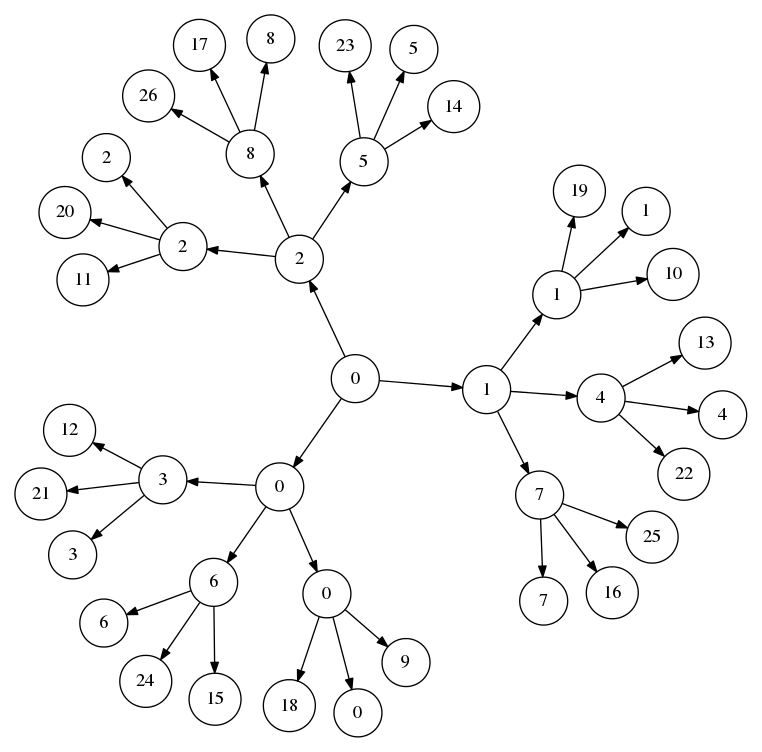
\includegraphics[width=0.85\linewidth]{images/drzewo.png}}
 \captionof{figure}{Rzekomo jest to drzewiasta struktura (niezbudowanego jeszcze) $\Z_3$.}
\end{Figure}

%%% skompilowane przez neato
% digraph G {
%     nodesep=0.3;
%     ranksep=0.2;
%     margin=0.1;
%     node [shape=circle];
%     edge [arrowsize=0.8];
% 	ae [label="0"]; 
% 	aq [label="0"]; 
% 	ar [label="1"]; 
% 	aw [label="2"]; 
% 	de [label="0"];
% 	dq [label="3"];
% 	dr [label="6"];
% 	dw [label="1"];
% 	ee [label="4"];
% 	eq [label="7"];
% 	er [label="2"];
% 	ew [label="5"];
% 	fe [label="8"];
% 	fq [label="0"];
% 	fr [label="9"];
% 	fw [label="18"];
% 	ge [label="3"];
% 	gq [label="12"];
% 	gr [label="21"];
% 	gw [label="6"];
% 	qe [label="15"];
% 	qq [label="24"];
% 	qr [label="1"];
% 	qw [label="10"];
% 	re [label="19"];
% 	rq [label="4"];
% 	rr [label="13"];
% 	rw [label="22"];
% 	se [label="7"];
% 	sq [label="16"];
% 	sr [label="25"];
% 	sw [label="2"];
% 	te [label="11"];
% 	tq [label="20"];
% 	tr [label="5"];
% 	tw [label="14"];
% 	we [label="23"];
% 	wq [label="8"];
% 	wr [label="17"];
% 	ww [label="26"];
% 	de -> fq;
% 	de -> fr;
% 	de -> fw;
% 	dq -> ge;
% 	dq -> gq;
% 	dq -> gr;
% 	dr -> gw;
% 	dr -> qe;
% 	dr -> qq;
% 	dw -> qr;
% 	dw -> qw;
% 	dw -> re;
% 	ee -> rq;
% 	ee -> rr;
% 	ee -> rw;
% 	eq -> se;
% 	eq -> sq;
% 	eq -> sr;
% 	er -> sw;
% 	er -> te;
% 	er -> tq;
% 	ew -> tr;
% 	ew -> tw;
% 	ew -> we;
% 	fe -> wq;
% 	fe -> wr;
% 	fe -> ww;
%     ae -> aq;
%     ae -> ar;
%     ae -> aw;
%     aq -> de;
%     aq -> dq;
%     aq -> dr;
%     ar -> dw;
%     ar -> ee;
%     ar -> eq;
%     aw -> er;
%     aw -> ew;
%     aw -> fe;
% }

 % gotowe
	\section{Klasyfikacja wymiernych norm}
Znamy \prawo{Gouvea\\3.1} już trzy różne rodzaje norm na ciele liczb wymiernych: rodzinę norm $p$-adycznych, klasyczną oraz trywialną wartość bezwzględną.
Naturalne pytanie, jakie powinniśmy sobie postawić, brzmi: czy są jeszcze jakieś?

Przypomnijmy: dwie normy na ciele są równoważne dokładnie wtedy, gdy ich metryki generują dokładnie takie same topologie.
Łatwiej powiedzieć niż sprawdzić, ale na szczęście mamy poniższy lemat.

\begin{lemat}
	Następujące warunki są równoważne dla dwóch norm na jednym ciele $\cialo$:
	\begin{enumx}
		\item topologie od norm pokrywają się, 
		\item $\|x\|_1 < 1$, wtedy i tylko wtedy gdy $\|x\|_2 < 1$, 
		\item istnieje stała $\alpha > 0$, że dla $x \in \cialo$ jest $\|x\|_1 = \|x\|_2^\alpha$.
	\end{enumx}
\end{lemat}

\begin{proof}
	Pokażemy ciąg implikacji $3 \Rightarrow 1 \Rightarrow 2 \Rightarrow 3$.
	
	($3 \Rightarrow 1$) $\|x-y\|_1 < r$, wtedy i tylko wtedy gdy $\|x-y\|_2 < r^{1:\alpha}$.
	Otwarte kule są nadal otwarte, choć nie zawsze o takim samym promieniu. 

	($1 \Rightarrow 2$) Z każdą topologią związane jest pojęcie zbieżności.
	Zauważmy, że $x^n$ dąży do zera dokładnie dla $\|x\| < 1$.
	
	($2 \Rightarrow 3$) Wybierzmy $y \in \cialo^\times$, takie że $\|y\|_1 < 1$.
	Warunek nr 2 mówi, że $\|y\|_2$ też jest mniejsze od jeden.
	Wskazujemy więc $\alpha > 0$ takie, by $\|y\|_1 = \|y\|_2^\alpha$.

	Weźmy $x \in \cialo^\times$.
	Jeśli $\|x\|_1 = \|y\|_1$, to drugie normy także są równe, w przeciwnym przypadku jedna z liczb $x/y$ lub $y/x$ miałaby drugą normę większą niż jeden, przeczyłoby to założeniu.
	Jeśli $\|x\|_1 = 1$, to (patrząc na $x$ lub $1/x$) widzimy $\|x\|_2 = 1$, wtedy równość $\|x\|_1 = \|x\|_2^\alpha$ zachodzi w próżni.

	Zastępując (w miarę potrzeby) $x$ przez jego odwrotność, możemy założyć $\|x\|_1 < 1$ i wziąć $\beta > 0$, by $\|x\|_1 = \|x\|_2^\beta$.
	Ustalmy naturalne $n, m$.
	Wtedy $\|x\|_1^n < \|y\|_1^m$, wtedy i tylko wtedy gdy $\|x\|_2^n < \|y\|_2^m$.
	Wzięcie logarytmów daje (po drobnych przekształceniach)
	\[
		\frac nm < \frac{\log \|y\|_1}{\log \|x\|_1} \iff \frac n m < \frac{\log \|y\|_2}{\log \|x\|_2}.
	\]

	Prawostronne ułamki są równe, więc $\|y\|_1 = \|y\|_2^\alpha$ i rzeczywiście $\alpha = \beta$.
\end{proof}

\begin{wniosek}
	Dwie normy, z których dokładnie jedna jest archimedesowa, nie są równoważne.
\end{wniosek}

\begin{wniosek}
	Normy $p$- i $q$-adyczne są równoważne, wtedy i tylko wtedy gdy $p = q$.
\end{wniosek}



\begin{definicja}
	Dwie normy spełniające dowolny z trzech warunków lematu nazywamy równoważnymi.
\end{definicja}

\begin{twierdzenie}[Ostrowski, 1916]
	Każda norma na $\Q$ jest dyskretna lub równoważna z $\|\cdot\|_p$, gdzie $p \le \infty$ jest liczbą pierwszą.
\end{twierdzenie}

\begin{proof}
	Niech $\|\cdot\|$ będzie nietrywialną normą na $\Q$.
	Pierwszy przypadek: archimedesowa (odpowiada normie $|\cdot|_\infty$).
	Weźmy więc najmniejsze dodatnie całkowite $n_0$, że $\|n_0\| > 1$.
	Wtedy $\|n_0\| = n_0^\alpha$ dla pewnej $\alpha > 0$.
	Wystarczy uzasadnić, dlaczego $\|x\| = |x|_\infty^\alpha$ dla każdej $x \in \Q$, a właściwie tylko dla $x \in \N $ (gdyż norma jest multiplikatywna).
	Dowolną liczbę $n$ można zapisać w systemie o podstawie $n_0$: $n = a_0 + a_1 n_0 + \dots + a_mn_0^m$, gdzie $a_m \neq 0$ i $0 \le a_j \le n_0-1$.
	\begin{align*}
		\|n\| & = \left\|\sum_{i=0}^m a_in_0^i\right\| \le \sum_{i=0}^m \left\|a_i\right\| n_0^{i \alpha} \le n_0^{m \alpha} \sum_{i = 0}^m n_0^{-i \alpha} \le n_0^{m \alpha} \sum_{i = 0}^\infty n_0^{-i \alpha} = C n_0^{m \alpha} %  n_0^{m \alpha} \frac{n_0^\alpha}{n_0^\alpha - 1}
	\end{align*}

	Pokazaliśmy $\|n\| \le Cn_0^{m \alpha} \le C n^\alpha$ dla każdego $n$, a więc w szczególności dla liczb postaci $n^N$ (gdyż $C$ nie zależy od $n$): $\|n\| \le C^{1/n}n^\alpha$.
	Idziemy z $N$ do nieskończoności, wtedy $C^{1/n}$ zbiega do jedynki i otrzymujemy półrówność $\|n\| \le n^\alpha$.

	Teraz trzeba pokazać nierówność w drugą stronę.
	Skorzystamy jeszcze raz z rozwinięcia.
	Skoro $n_0^{m+1} > n \ge n_0^m$, to nie kłamczymy pisząc $\|n+n_0^{m+1} - n\| \le \|n\| + \|n_0^{m+1} - n\|$, 
	
	Wnioskujemy stąd, że $\|n\| \ge n_0^{(m+1) \alpha} - \|n_0^{m+1} - n\| \ge n_0^{(m+1)\alpha} - (n_0^{m+1} - n)^\alpha$.
	Skorzystaliśmy tutaj z nierówności udowodnionej wyżej.
	Wiemy, że $n \ge n_0^m$, zatem
	\begin{align*}
		\|n\| & \ge n_0^{(m+1)\alpha} - (n_0^{m+1} - n_0^m)^\alpha = n_0^{(m+1) \alpha} [1 - (1 - 1 : n_0)^\alpha] = C' n^\alpha.
	\end{align*}

	Od $n$ nie zależy $C' = 1 - (1-1:n_0)^\alpha$, jest dodatnia i przez analogię do poprzedniej sytuacji możemy pokazać $\|n\| \ge n^\alpha$.
	Wnioskujemy stąd, że $\|n\| = n^\alpha$ i $\|\cdot\|$ jest równoważna najzwyklejszej wartością bezwzględną.

	Załóżmy, że $\|\cdot\|$ jest niearchimedesowa.
	Wtedy $\|n\| \le 1$ dla całkowitych $n$.
	Ponieważ $\|\cdot\|$ jest nietrywialna, musi istnieć najmniejsza l. całkowita $n_0$, że $\|n_0\| < 1$.
	Zacznijmy od tego, że $n_0$ musi być l. pierwszą: gdyby zachodziło $n_0 = a \cdot b$ dla $1 < a,b < n_0$, to $\|a\| = \|b\| = 1$ i $\|n_0\| < 1$ (z minimalności $n_0$) prowadziłoby do sprzeczności.
	Chcemy pokazać, że $\|\cdot\|$ jest równoważna z normą $p$-adyczną, gdzie $p := n_0$.
	W następnym kroku uzasadnimy, że jeżeli $n \in \Z$ nie jest podzielna przez $p$, to $|n| = 1$.
	Dzieląc $n$ przez $p$ z resztą dostajemy $n = ap + b$ dla $0 < b < p$.
	Z minimalności $p$ wynika $\|b\| = 1$, zaś z $\|a\| \le 1$ ($\|\cdot\|$ jest niearchimedesowa) i $\|p\| < 1$: $\|ap\| < 1$.
	,,Wszystkie trójkąty są równoramienne'', więc $\|n\| = 1$.
	Wystarczy więc tylko zauważyć, że dla $n \in \Z$ zapisanej jako $n = p^v n'$ z $p \nmid n'$ zachodzi $\|n\| = \|p\|^v \|n'\| = \|p\|^v \le 1$.
\end{proof}

\begin{historia}[Ostrowski Aleksander]\end{historia}

Często w starciu z  teorioliczbowymi problemami warto pracować ze wszystkimi liczbami pierwszymi jednocześnie, to znaczy korzystać z informacji, jakich dostarczają różne normy na $\Q$.
Oto fundamentalny przykład, który pokazuje przy okazji, że $\infty$ też zasługuje być nazywana liczbą pierwszą.

\begin{fakt}[,,adelizm'' 1]
	Gdy $x \in \Q^\times$, to $\prod_{p \le 2} |x|_p = 1$.
\end{fakt}

\begin{proof}
	Wystarczy użyć zasadniczego twierdzenia arytmetyki.
\end{proof}

Podobne stwierdzenie jest prawdziwe dla skończonych rozszerzeń $\Q$, chociaż wtedy trzeba dołożyć po jednej ,,nieskończoności'' za każde włożenie w $\R$ (albo $\C$).
Zajmiemy się tym przypadkiem nieco później. % gotowe
	\section{Łatanie podziurawionych ciał}
Przypomnienie: $\R$ jest uzupełnieniem $\Q$, to znaczy norma $|\cdot|_\infty$ przedłuża się na $\R$, $\R$ jest zupełne z metryką od niej i $\Q$ leży gęsto w $\R$. Uzupełnianie jest konieczne, gdyż

\begin{lemat}
	Ciało $\Q$ z nietrywialną normą nie jest zupełne.
\end{lemat}

\begin{proof}
	Dzięki twierdzeniu Ostrowskiego wystarczy sprawdzić $p$-adyczne normy.
	Niech $p \neq 2$ będzie pierwsza, zaś $y \in \Z$ taka, że nie jest kwadratem, nie dzieli się przez $p$ i równanie $x^2 = y$ ma rozwiązanie w $\Z/p\Z$.
	Stosowne $y$ zawsze istnieje: wystarczy powiększyć jakiś kwadrat z $\Z$ o krotność $p$.
	
	Niech $y_0$ będzie dowolnym rozwiązaniem równania, $y_n$ ma być równe $x_{n-1}$ modulo $p^n$ oraz $y_n^2 = y$ (modulo $p^{n+1}$).
	Tak skonstruowany ciąg Cauchy'ego nie ma granicy, oto stosowne rachunki:
	\begin{align*}
		y_n & = y_{n-1} + \lambda_n p^n \\
		y_n^2 & = y_{n-1}^2 + 2 y_{n-1} \lambda_n p^n + \lambda_n^2 p^{2n} \\
		\lambda_n & = (y - y_{n-1}^2)(2y_{n-1} p^n)^{-1} \pmod p
	\end{align*}
	
	Jest Cauchy'ego ($|y_{n+1} - y_n| \le p^{-n-1}$) i nie ma granicy ($|y_n^2 - y| \le p^{-n-1}$, ale pierwiastek z $y$, jedyny kandydat, nie istnieje).
	Gdy $p = 2$, to zastępujemy pierwiastek kwadratowy sześciennym.
\end{proof}

Zbiór ciągów Cauchy'ego oznaczmy przez $C$.
Można na nim zadać strukturę pierścienia (przemiennego i z jedynką) przez punktowe dodawanie oraz mnożenie.
Wprowadzamy ideał $N$, do którego należą ciągi zbieżne do zera.

\begin{lemat}
	Ideał $N \trianglelefteq C$ jest maksymalny.
\end{lemat}

\begin{proof}
Ustalmy ciąg $(x_n) \in C \setminus N$ oraz ideał $I = \langle (x_n), N \rangle$.
Od pewnego miejsca $x_n$ nie jest zerem, zatem $y_n = 1/x_n$ od tego miejsca, $0$ wcześniej ma sens.
Ciąg $y_n$ jest Cauchy'ego:
\[
	|y_{n+1} - y_n| = \frac{|x_{n+1} - x_n|}{|x_nx_{n+1}|} \le \frac{|x_{n+1}-x_n|}{\varepsilon^2} \to 0.
\]
Ale $(1) - (x_n)(y_n) \in N$, więc $I = C$.
\end{proof}

\begin{definicja}
	Ciało liczb $p$-adycznych to $\Q_p := C / N$.
\end{definicja}

\begin{lemat}
	Ciąg $|x_n|_p$ jest stacjonarny, gdy $(x_n) \in C \setminus N$.
\end{lemat}

\begin{proof}
	Można znaleźć takie liczby $\varepsilon, N_1$, że $n \ge N_1$ pociąga $|x_n| \ge \varepsilon > 0$.
	Z drugiej strony istnieje taka $N_2$, że $n, m \ge N_2$ pociąga $|x_n - x_m| < \varepsilon$.
	Połóżmy więc $N = \max\{N_1, N_2\}$.
	Wtedy $n, m \ge N$ pociąga $|x_n - x_m| < \max\{|x_n|, |x_m|\}$, a to oznacza, że $|x_n| = |x_m|$.
\end{proof}

Dzięki temu następująca definicja nie jest bez sensu:

\begin{definicja}
	Gdy $(x_n) \in C$ reprezentuje $x \in \Q_p$, przyjmujemy $|x|_p := \lim_{n \to \infty} |x_n|_p$.
\end{definicja}

\begin{lemat}
	Obraz $\Q \hookrightarrow \Q_p$ po włożeniu jest gęsty.
\end{lemat}

\begin{proof}
	Chcemy pokazać, że każda otwarta kula wokół $x \in \Q_p$ kroi się z obrazem $\Q$, czyli zawiera ,,stały ciąg''.
	Ustalmy kulę $\kula(x, \varepsilon)$, ciąg Cauchy'ego $(x_n)$ dla $x$ i $\varepsilon' < \varepsilon$.
	Dzięki temu, że ciąg jest Cauchy'ego, możemy znaleźć dla niego indeks $N$, że $n, m \ge N$ pociąga $|x_n - x_m| < \varepsilon'$.
	Rozpatrzmy stały ciąg $(y)$ dla $y = x_N$.
	Wtedy $|x - (y)| < \varepsilon$, gdyż $x - (y)$ odpowiada ciąg $(x_n-y)$.
	Ale $|x_n - x_N| < \varepsilon'$ i $\lim_{n \to \infty}|x_n - y| \le \varepsilon' < \varepsilon$.
\end{proof}

\begin{fakt}
	Ciało $\Q_p$ jest zupełne.
\end{fakt}

\begin{proof} 
	Ustalmy $x_n$, ciąg Cauchy'ego elementów $\Q_p$.
	Obraz $\Q$ w $\Q_p$ jest gęsty, a zatem można znaleźć liczby wymierne $q_n$, że $|x_n - (q_n)| \to 0$ (w ciele $\Q_p$).
	Okazuje się, że liczby $q_n$ same tworzą ciąg Cauchy'ego i to właśnie on jest granicą $x_n$.
\end{proof}

\begin{fakt}
	Własności pierścienia waluacji $\{x \in \Q_p : |x|_p \le 1\}$:
	\begin{enumx}
		\item pierścień ,,$\Z_p$'' jest lokalny; ideał $p \Z_p$ jest maksymalny
		\item $\Q \cap \Z_p = \Z_{(p)} = \{\frac yz \in \Q: p \nmid z\}$
		\item włożenie $\Z \hookrightarrow \Z_p$ ma gęsty obraz: jeśli $x \in \Z_p$ i $n \ge 1$, to istnieje jedyna $x_n \in \Z \cap [0, p^n- 1]$, że $|x-x_n| \le p^{-n}$.
		\item każdy $x \in \Z_p$ jest granicą ciągu Cauchy'ego $x_n \in \Z$, którego wyrazy spełniają $0 \le x_n \le p^n-1$, $p^{n-1} \mid (x_n - x_{n-1})$.
	\end{enumx}
\end{fakt}

\begin{proof}
	Pierścień $\Z_p$ jest lokalny, jak inne pierścienie waluacji.
	Ideał waluacji ma $p$ za generator, bo $|x| < 1$ wtedy i tylko wtedy gdy $|x/p| \le 1$, czyli $x \in p\Z_p$.
	Ideał waluacji zawiera się w $p\Z_p$ i jest maksymalny, czyli jest nim po prostu $\Z_p$.

	Niech $x \in \Z_p$, $n \ge 1$.
	Wskażmy $\frac yz \in \Q$, że $|x-\frac yz| \le p^{-n}$.
	Skoro $|y/z| \le \max (|x|, |x-y/z|) \le 1$ (czyli $p \nmid z$), to istnieje $z' \in \Z$, że $zz' \equiv 1$ mod $p^n$.
	To oznacza, że $|y/z-yz'| \le p^{-n}$ i $yz' \in \Z$.
	Zastąpiliśmy ułamek liczbą całkowitą.

	Wybierając $x_n$, jedyną całkowitą, że $0 \le x_n \le p^n-1$ i $x_n = yz'$ modulo $p^n$, dostajemy $|x - x_n| \le p^{-n}$.
	Ostatni punkt wynika z przedostatniego.
\end{proof}

\begin{wniosek}
	Zbiory $p^n\Z_p$ to układ otoczeń dla zera kryjący $\Q_p = \Z_p[1/p]$ ($n \in \Z$).
	Ciąg $0 \to \Z_p \to \Z_p \to \Z/p^n\Z \to 0$ (najpierw mnożymy przez $p^n$, później rzutujemy) jest dokładny, a strzałki ciągłe, więc $\Z_p^+$ jest beztorsyjna i ${\Z_p}/{p^n \Z_p} \cong {\Z}/{p^n \Z}$.
\end{wniosek}
 % gotowe
	\section{Lemat Hensela o podnoszeniu}
,,Lemat Hensela'' opisuje jedną z ważniejszych algebraicznych cech ciał udających $\Q_p$ (zupełnych oraz z niearchimedesową normą).
Orzeka mianowicie, że w pewnych warunkach można łatwo sprawdzić, czy wielomian ma pierwiastki w $\Z_p$.

\begin{twierdzenie}[lemat Hensela]
	Każde z zer $x_1 \in \Z_p$ (modulo $p \Z_p$) dla wielomianu $f(x) \in \Z_p[x]$, że $f'(x_1) \not \equiv 0$ mod $p \Z_p$ można podnieść do prawdziwego zera $x$, które przystaje do $x_1$ mod $p\Z_p$.
	Co więcej, zero to jest jednoznacznie wyznaczone.
\end{twierdzenie}

\begin{proof}
	Wskażemy ciąg Cauchy'ego zbieżny do $x$ przy użyciu ,,metody Newtona'' ($x_n$), taki że $f(x_n) \equiv 0$ mod $p^n$ i $x_n \equiv x_{n+1}$ mod $p^n$.
	Mamy $x_1$, chcemy $x_2 = x_1 + y_1 p$ dla $y_1 \in \Z_p$.

	Widzimy, że $f(x_2) = f(x_1) + f'(x_1) y_1p + p^2 \cdot r_2$ (gruz).
	Szukamy $y_1$, dla którego $f(x_1) + f'(x_1) y_1p \equiv 0$ mod $p^2$, czyli $z_1 + f'(z_1) y_1 \equiv 0$ mod $p$, gdzie $f(x_1) = pz_1$. 
	Rozwiązaniem jest $y_1 \equiv -z_1 f'(x_1)^{-1}$ mod $p$.
	Uważny Czytelnik zauważy, że skoro z $x_1$ można dostać $x_2$, to z $x_n$ można dostać $x_{n+1}$.
\end{proof}

W dowodzie skorzystaliśmy ze wzoru Taylora:

\begin{fakt}
	Dla wielomianu $f(x)$ nad ciałem $\cialo$ charakterystyki zero jest $f(x+h) = f(x) + f'(x)h + f''(x)h^2 / 2 + \ldots$, $x, h \in \cialo$.
\end{fakt}

\begin{proof}
	Nieustanne różniczkowanie sprawia, że wielomian $f$ kiedyś stanie się zerem.
	Wystarczy porównać współczynniki przy $x^j$ po obu stronach.
\end{proof}

\begin{historia}[Hensel Kurt]\end{historia}

Założenie z lematu ($f'(x) \not\equiv 0$) można osłabić, choćby do $|f(x)| < |f'(x)|^2$.
Dowód podał już w 1846 Schöneman (?).
Już wkrótce i tak przetłumaczymy wszystko na język waluacji.

\begin{historia}[Schönemann Theodor]\end{historia} %oddkrył lemat Hensela przed Henselem, prawo wzajemności Scholza przed Scholzem oraz kryterium Eisensteina przed Eisensteinem.

Wyznaczymy teraz pierwiastki jedności w $\Q_p$ wielomianem $f(x) = x^m - 1$ z pochodną $f'(x) = mx^{m-1}$.
Aby spełnione było drugie założenie z lematu, musimy mieć $p \nmid m$ (zakładamy to) i pozostaje sprawdzić pierwsze założenie.

\begin{lemat}
	Niech $p \nmid m$.
	Istnieje taka całkowita $n$, że $n^m \equiv 1$ mod $p$ (ale $n \not\equiv 1$ mod $p$), wtedy i tylko wtedy gdy $(m, p - 1) > 1$.
	Dla każdego $n$, najmniejsza $m$ o żądanych własnościach dzieli $p-1$.
\end{lemat}

\begin{proof}
	Załóżmy istnienie $n$.
	Rząd $n$ w $(\Z / p\Z)^\times$ dzieli zarówno $m$, jak i $p-1$, zatem $(m, p-1) > 1$, chyba że $n \equiv 1$ mod $p$.
	Najmniejsze $m$ musi dzielić NWD, a z nim także $p-1$.

	Odwrotnie, w grupie cyklicznej rzędu $p-1$ istnieje element każdego rzędu, który dzieli $p-1$, a taka jest $(\Z/p\Z)^\times$.
\end{proof}

Lemat Hensela daje:

\begin{fakt}
	Jeżeli naturalna $m$ nie dzieli się przez pierwszą $p$, to w $\Q_p$ istnieje $m$-ty pierwiastek pierwotny z jedynki, wtedy i tylko wtedy gdy $m$ dzieli $p-1$.
\end{fakt}

Nie wykluczyliśmy jeszcze istnienia $p^n$-tych pierwiastków jedności w $\Q_p$, uda się to po poznaniu logarytmu.
Pierwiastki jedności w $\Q_p$ dla $p \ge 3$ tworzą grupę $\mu_{p-1}$ o $p-1$ elementach.

,,Jednostka urojona'', czyli kwadratowy pierwiastek z $-1$ w $\Q_p$ istnieje dokładnie wtedy, gdy $\frac 1 2(p-1)$ jest jeszcze parzysta, czyli dla $p$ postaci $4k+1$.

Teraz zajmiemy się kwadratami.

\begin{fakt}
	Jeśli tylko $p > 2$, to każda $p$-adyczna jedność $y$, dla której istnieje $z$, że $z^2 \equiv y$ mod $p \Z_p$, jest kwadratem czegoś z $\Z_p^\times$.
\end{fakt}

\begin{proof}
	Lemat Hensela dla $x^2 - y$, bo $p \neq 2$ i $y \in \Z_p^\times$ pociągają $2 z \not\equiv 0$ mod $p$.
\end{proof}

\begin{wniosek}
	$\{x^2 : x \in \Q_p\} = \{p^{2n} y^2 : n \in \Z, y \in \Z_p^\times\}$, a grupa ilorazowa $\Q_p^\times / (\Q_p^\times)^2$ ma rząd cztery i reprezentantów warstw $\{1, p, c, cp\}$, przy czym $c \in \Z_p^\times$ jest dowolnym elementem, którego redukcja mod $p$ nie jest resztą kwadratową.
\end{wniosek}

\begin{proof}
	Własności reszt kwadratowych.
\end{proof}

Dla $\R$ jest inaczej: dokładnie nieujemne liczby to kwadraty, zaś $\R^\times/(\R^\times)^2$ odpowiada $\{-1, 1\}$. Co może się dziać w $\Q_2$? Potrzebna jest mocniejsza forma lematu, albowiem $f'(x) = 2x$ jest wielokrotnością dwójki.

\begin{fakt}
	Każda liczba $y \in 1 + 8\Z_2 \subseteq \Z_2$, jest kwadratem w $\Z_2$.
	Odwrotnie, $2$-adyczna jedność i kwadrat przystaje do $1$ mod $8$.
	Zatem $\Q^\times_2 / (\Q^\times_2)^2$ ma rząd osiem, odpowiada jej $\{\pm 1, \pm 2, \pm 5, \pm 10\}$.
\end{fakt}

\begin{proof}
	Wystarczy użyć wzmocnionego lematu.
\end{proof}

Lemat Hensela mówi, że jeżeli wielomian dzieli się przez $x - x_0$: $f(x) \equiv (x - x_0) g(x)$ mod $p$, to w podobny sposób daje się rozłożyć także w $\Z_p[x]$.
Warunek nałożony na pochodną dopuszcza jedynie pojedyncze pierwiastki.
Teraz osłabimy to założenie do względnej pierwszości.

Przez $\overline w$, oznaczymy redukcję współczynników wielomianu $w \in \Z_p[x]$ modulo $p$.

\begin{definicja}
	Wielomiany $q, r$ są względnie pierwsze modulo $p$, gdy $(\overline q, \overline r) = 1$ w $\mathbb F_p[x]$.
\end{definicja}

Istnieją wtedy $a, b \in \Z_p[x]$, że $aq + br \equiv 1$ mod $p$.

\begin{twierdzenie}
	Niech dla wielomianu $f(x) \in \Z_p[x]$ istnieją dwa względnie pierwsze mod $p$ wielomiany: $g_1$, $h_1 \in \Z_p[x]$, przy czym $g_1$ jest unormowany i $f(x) \equiv (g_1h_1)(x)$ mod $p$.
	Wtedy istnieją takie $g(x), h(x) \in \Z_p[x]$, że $g$ jest unormowany, $g$ i $g_1$ oraz $h$ i $h_1$ przystają do siebie mod $p$ oraz $f(x) = (gh)(x)$.
\end{twierdzenie}

\begin{proof}
	Postępujemy jak wcześniej: znajdujemy przybliżone rozwiązanie i próbujemy przejść do granicy. 

	Niech $d$ będzie stopniem $f$, zaś $m$: stopniem $g_1$.
	Możemy założyć, że $\deg h_1 \le d - m$.
	Potrzebne są nam dwa ciągi, $g_n$ i $h_n$ (wielomiany), że: każdy $g_n$ jest unormowany, $g_{n+1} \equiv g_n$ mod $p^n$ oraz $h_{n+1} \equiv h_n$ mod $p^n$, a przy tym $f \equiv g_n h_n$ mod $p^n$.
	Wielomiany $h, g$ otrzymamy przez przejście do granicy.

	Mamy już $g_1, h_1$.
	Musi zachodzić $g_2 = g_1 + pr_1$, a przy tym $h_2 = h_1 + ps_1$.
	Po podstawieniu do równania $f \equiv g_2h_2$ mod $p^2$ i uproszczeniu otrzymamy $f - g_1 h_1 = pk_1$ dla $k_1 \in \Z_p[x]$.
	Dalsze uproszczenie do $p k_1 \equiv pr_1 h_1 + p s_1 g_1$ mod ${p^2}$ sprawia, że chcemy podzielić przez $p$.

	Skoro $g_1, h_1$ są względnie pierwsze mod $p$, to istnieją $a, b$ (wielomiany nad $\Z_p$), że $ag_1 + bh_1 \equiv 1$ mod $p$.
	Rozpatrzmy nowe wielomiany, $\overline r_1 = bk_1$ i $\overline s_1 = ak_1$.
	Wiemy już, że
	\[
		\overline r_1 h_1 + \overline s_1 g_1 \equiv k_1 \pmod p.
	\]

	Podzielmy $\overline r_1$ przez $g_1$; niech $r_1$ będzie resztą: $r_1 = g_1 q + r_1$.
	Rzecz jasna $\deg r_1 < \deg g_1$.
	Ale jeśli położymy $s_1 = \overline s_1 + h_1q$, to wszystko będzie grać:
	\begin{align*}
	\ldots & = r_1 h_1 + s_1 g_1
	\equiv (\overline r_1 - g_1 q)h_1 + (\overline s_1 + h_1 q)g_1 \\
	& \equiv \overline r_1 h_1 - g_1 h_1 q + \overline s_1 g_1 + g_1 h_1 q
	\equiv \overline r_1 h_1 + \overline s_1 g_1 \\
	& \equiv k_1 \pmod p.
	\end{align*}

	Tak pokazaliśmy, że $g_2$ oraz $h_2$ istnieją.
	Skoro przystają do $g_1$ i $h_1$ mod $p$, to również są względnie pierwsze mod $p$ i możemy wykonać kolejny krok ,,indukcyjny''.
\end{proof}
 % gotowe
	\section{Regionalnie czy wszechstronnie?}
Jednym z wniosków lematu Hensela jest to, że dla wielomianu o współczynnikach całkowitych łatwo sprawdzić, czy ma zera w $\Z_p$ (bo wystarczy szukać ich w $\Z/p\Z$), podobnie w $\R$.
Istnienie pierwiastka w $\Q$ pociąga ,,to samo'' w każdym $\Q_p$ ($p \le \infty$).
Trzeba o tym myśleć tak: ciała $p$-adyczne są odpowiednikami ciał rozwinięć Laurenta i dają ,,lokalną'' informację ,,blisko'' $p$.
Fakt, że pierwiastki przenoszą się z $\Q$ do $\Q_p$ oznacza bowiem, że ,,globalny'' pierwiastek jest też ,,lokalnym'' dla każdego $p$, czyli ,,wszędzie''.
Ciekawe pytanie brzmi, kiedy można to odwrócić.

\begin{fakt}
	Liczba $x \in \Q$ jest kwadratem wtedy i tylko wtedy, gdy jest kwadratem w każdym $\Q_p$, $p \le \infty$.
\end{fakt}

Zbyt niejasne, żeby nazwać twierdzeniem:

\begin{fakt}[reguła lokalno-globalna]
	Istnienie rozwiązań w $\Q$ (lub ich brak) dla równania diofantycznego można stwierdzić na podstawie istnienia (lub nie) rozwiązań w $\Q_p$.
\end{fakt}

Niestety, $(x^2 -2)(x^2-17)(x^2-34) = 0$ ma pierwiastki w każdym z $\Q_p$, ale nie w $\Q$. Inny przykład: $x^4 - 17 = 2y^2$. Na szczęście nie wszystko stracone.

\begin{twierdzenie}[Hasse, Minkowski]
	Forma kwadratowa $F$ nad $\cialo$ (ciałem liczbowym jak $\Q$) reprezentuje nietrywialnie zero w $\cialo$, wtedy i tylko wtedy gdy reprezentuje je w każdym uzupełnieniu $\cialo$.
\end{twierdzenie}

\begin{proof}
	Zbyt trudny (przez wyrwy w wiedzy o kwadratowych formach), nawet dla samego $\cialo = \Q$.
	Można go jednak znaleźć w pierwszej połowie książki Serre'a (\cite{serre73})
\end{proof}

\begin{historia}[Hasse Helmut]\end{historia}
\begin{historia}[Minkowski Hermann]\end{historia}
\color{black}

Ograniczymy się do rozwiązania tylko jednego równania: $ax^2 + by^2 + cz^2 = 0$ dla wymiernych $a, b,c $.
Poczynimi kilka założeń: $abc \neq 0$ jest bezkwadratowa oraz $a,b,c \in \Z$, gdyż możemy.
Wynika stąd, że $a,b,c$ są parami względnie pierwsze i różnych znaków (patrz $p= \infty$!).

\begin{fakt}
	Jeśli liczba pierwsza $p > 2$ nie dzieli $abc$, to istnieją liczby $x_0, y_0, z_0 \in \Z$, że $ax_0^2 + by_0^2 + cz_0^2 = 0$, a przy tym $p$ nie dzieli wszystkich trzech ($x_0, y_0, z_0$).
\end{fakt}

\begin{proof} %Specjalny przypadek twierdzenia Chevalleya-Warninga.
	Gdy $x, y, z$ przebiegają przez całkowite od $0$ do $p-1$, to istnieje $p^3$ trójek $(x,y,z)$.
	Ile z nich pasuje do równania?
	Brudna sztuczka: $(ax^2+by^2+cx^2)^{p-1}$ jest równe $1$, gdy trójka nie jest rozwiązaniem (i $0$ w przeciwnym przypadku), wynika to z MTF.
	Liczba nierozwiązań to $\sum_{p^3} (ax^2+by^2+cz^2)^{p-1}$ (ale modulo $p$!).
	Rozwijamy potęgi i dostajemy sumy postaci $\sum \lambda x^{2i}y^{2k}z^{2l}$ z $2i+2k+2l = 2(p-1)$ i $\lambda \in \Z$.
	Każda z nich jest zerem modulo $p$: 
	przynajmniej jedna z $2i, 2k, 2l$ jest mniejsza od $p-1$ (powiedzmy, $2i$).
	Wtedy nasza suma to
	\[
		\sum_{(y,z)} \left(\lambda y^{2k}z^{2l} \sum_{x} x^{2i}\right).
	\]

	Przywołujemy poniższy lemat.
	Skoro $p$ dzieli $N$ (liczbę nierozwiązań), to dzieli także $p^3 - N$.
	Znamy jedno rozwiązanie (trywialne), zatem istnieją inne.
	Był to specjalny przypadek tw. Chevalleya i Warninga.
\end{proof}

\begin{lemat}
	Jeśli $0 \le n \le p-1$, to $p$ dzieli $\sum_{i=0}^{p-1} i^n$.
\end{lemat}

\begin{proof}
Wybierzmy takie $y$, że $y^n \not\equiv 1$ mod $p$.
Wtedy
\[
	0 \equiv \sum_{i=0}^{p-1} i^n - \sum_{i=0}^{p-1} (yi)^n = (1-y^n) \sum_{i = 0}^{p-1} i^n \qedhere
\]
\end{proof}

Znając rozwiązanie $(x_0,y_0, z_0)$ ,,mod $p$'' wiemy, że $p \nmid x_0$ (bez straty ogólności).
Znamy rozwiązanie wielomianowego $aX^2 + by_0^2 + cz_0^2 = 0$ modulo $p$, $x_0$.
Z naszymi założeniami lemat Hensela wskaże $x \in \Z_p$, pierwiastek równania, a także rozwiązanie pierwotnego: $(x, y_0, z_0)$.

To jeszcze nie koniec.
Załóżmy teraz, że $p = 2$, ale $a,b,c$ są nieparzyste.
Gdy istnieje rozwiązanie $(x,y,z) \in \Q_2^3$, to możemy założyć, że nie wszystkie leżą w $2\Z_2$ (innymi słowy, $\max\{|x|_2, |y|_2, |z|_2\} =1$).
Po redukcji mod $2\Z_2$ widzimy, że $y,z$ są jednościami $2$-adycznymi, $x$ dzieli się przez $2$.
Kwadrat $2$-adycznej jedności leży w $1+4\Z_2$, zaś kwadrat czegoś z $2\Z_2$ leży w $4\Z_2$. Redukując modulo $4\Z_2$ dostajemy więc: $b+ c \equiv 0$ mod $4$.
Okazuje się, że warunek ten jest nie tylko konieczny, ale też wystarczający.

\begin{lemat}
	Równanie $aX^2 + bY^2 + cZ^2 = 0$ ma nietrywialne rozwiązanie w $\Q_2$, gdy $2 \nmid abc$ i $4$ dzieli sumę dwóch z $a, b, c$.
\end{lemat}

\begin{proof}
	Szukamy początkowego rozwiązania $(x_0, y_0, z_0)$, dla którego $8 \mid ax_0^2 + by_0^2 + cz_0^2$.
	Jeśli $8 \mid a+b$, to kładziemy $x_0 = 1$, $y_0 = 1$, $z_0= 0$. Jeśli nie, to $z_0 = 2$, $x_0 = y_0 = 1$.
	Stosujemy lemat Hensela.
\end{proof}

\begin{lemat}
	Równanie $aX^2 + bY^2 + cZ^2 = 0$ ma nietrywialne rozwiązanie w $\Q_2$, gdy jedna z $a, b, c$ jest parzysta, zaś suma dwóch lub trzech z nich dzieli się przez 8.
\end{lemat}

\begin{proof}
	Załóżmy, że $2$ dzieli tylko $a$ oraz że $ax^2 + by^2 + cz^2 = 0$.
	Możemy przyjąć, że któraś z $x, y,z$ jest $2$-adyczną jednością, zaś wszystkie leżą w $\Z_2$.
	Kwadrat $2$-adycznej jedności leży w $1 + 8 \Z_2$, zatem $0 = ax^2 + by^2 + cz^2 \equiv b +c$ (mod $8$), jeśli $x \in 2\Z_2$ (wtedy $y,z$ muszą być $2$-adycznymi jednościami).

	Jeśli $x$ jest $2$-adyczną jednością, to $y, z$ i tak też muszą nimi być, co prowadzi do $a+b+c \equiv 0$ mod $8$.
	Twierdzenie odwrotne jest prawdziwe na mocy uogólnionego lematu Hensela.
\end{proof}

\begin{lemat}
	Jeżeli $p \neq 2$ dzieli $a$, to równanie ma nietrywialne rozwiązanie dokładnie wtedy, gdy $-b/c$ to kwadratowa reszta mod $p$.
\end{lemat}

\begin{proof}
	Ponownie, lemat Hensela.
\end{proof}

\begin{fakt}
	Niech liczby $a,b,c \in \Z$ będą parami względnie pierwsze, bezkwadratowe.
	Równanie $ax^2+by^2+cz^2 = 0$ posiada w $\Q$ nietrywialne rozwiązania, wtedy i tylko wtedy gdy:
	\begin{enumx}
		\item ($a,b,c$ nie są tego samego znaku)
		\item każdy nieparzysty dzielnik pierwszy liczby $a$ posiada $r \in \Z$, że $p \mid b+r^2c$, podobnie dla $b$ i $c$
		\item jeśli $2 \nmid abc$, to $4$ dzieli sumę pewnych dwóch z $a$, $b$, $c$.
		\item jeśli $2 \mid a$, to $8$ dzieli $b+c$ lub $a+b+c$ (podobnie $b$ i $c$).
	\end{enumx}

	Pierwszy warunek wynika z pozostałych.
\end{fakt}

Bezpośredni dowód można znaleźć w rozdziałach 3 -- 5 książki [Cas91].
Strategią jest użycie trzech warunków, a także ,,geometrii liczb'' Minkowskiego do pokazania, że możliwe jest znalezienie rozwiązania $(x, y, z)$ spełniającego nierówność
\[
	|a| x^2 + |b| y^2 + |c| z^2 < 4 |abc|.
\]
 % gotowe
	\section{Normowa niezależność}
Zaprezentujemy teraz pogląd Casselsa na temat niezależności nierównoważnych norm.
Co dokładnie przez to rozumiemy, stanie się jasne natychmiast po udowodnieniu lematu.

\begin{lemat}
	Niech nietrywialne normy $|\cdot|_1, \ldots, |\cdot|_m$ będą parami nierównoważne (na ciele $\cialo$).
	Istnieje wtedy $x \in \cialo$, że $|x|_1 > 1$, ale $|x|_2, \ldots, |x|_m < 1$.
\end{lemat}

\begin{proof}
	Indukcyjny względem $m$.
	Gdy $m = 2$, istnieją $y, z \in \cialo$, takie że $|y|_1, |z|_2 < 1$ oraz $|y|_2, |z|_1 \ge 1$.
	Poszukiwanym jest wtedy $x = zy^{-1}$.
	
	Jeżeli $m > 2$, to z założenia indukcyjnego mamy $y \in \cialo$, że $|y|_1 > 1$, $|y|_i < 1$ ($2 \le i \le m-1$).
	Z drugiej strony istnieje $z \in \cialo$, że $|z|_1 > 1$, $|z|_m < 1$.
	Rozpatrujemy trzy przypadki.

	Jeżeli $|y|_m < 1$, to $x = y$.
	Jeżeli $|y|_m = 1$, to $x = y^nz$ dla dużego $n$.
	Jeżeli $|y|_m > 1$, to $x = y^n z (1 + y^n)^{-1}$ dla dużego $n$.
	Mamy bowiem
	\[
		\frac{y^n}{1 + y^n} \to \begin{cases} 
		1 & \text{dla } |\cdot|_1 \text{ oraz } |\cdot|_m, \\
		0 & \text{w przeciwnym razie.}
		\end{cases} \qedhere
	\]
\end{proof}

\begin{fakt}
	Przy założeniach lematu, $x_1, \ldots, x_m \in \cialo$ oraz $\varepsilon > 0$ (rzeczywistym), istnieje $x \in \cialo$, że jednocześnie spełniona jest każda z nierówności $|x-x_i|_i < \varepsilon$.
\end{fakt}

\begin{proof}
	Z lematu wynika istnienie takich $y_i \in \cialo$, że $|y_i|_i > 1$, $|y_i|_k < 1$ ($k \neq i$).
	Wystarczy położyć
	\[
		x = \lim_{n \to \infty} \sum_{i=1}^m \frac{y_i^n}{1 + y_i^n} x_i. \qedhere
	\]
\end{proof}

Związane jest to z chińskim twierdzeniem o resztach.
Mówi ono, że gdy $x_i \in \Z$ są dane, $p_i$ parami różne (i pierwsze), zaś $m_i$ naturalne, to układ ,,kongruencji''
\[
	|x - x_i|_i \le p_i^{-m(i)}
\]
ma rozwiązanie nie tylko w $\Q$, ale także $\Z$.
Nasz fakt można jednak wzmocnić, gdy $\cialo$ jest algebraicznym ciałem liczbowym (uczynimy to, ale jeszcze nie teraz).

Przedstawimy teraz obrazowo niezależność.

\begin{fakt}
	Odwzorowanie przekątniowe ma gęsty obraz, kiedy $\cialo_i$ uzupełnia $\cialo$ względem nierównoważnych parami norm.
	\[
		\Delta: \cialo \hookrightarrow \prod_i \cialo_i
	\]
\end{fakt}

\begin{proof}
	Ustalmy elementy $x_i \in \cialo_i$ dla $1 \le i \le n$.
	Istnieją wtedy $y_i \in \cialo$, że $|x_i-y_i|_i < \varepsilon$ dla ustalonego $\varepsilon > 0$.
	Mamy takie $z \in \cialo$, że $|z - y_i|_i < \varepsilon$, zatem $|z - x_i|_i < 2 \varepsilon$ (na mocy poprzedniego faktu).
\end{proof} % gotowe

\chapter{Analiza}
Liczne podobieństwa między ciałami $\R$ oraz $\Q_p$ (lokalna zwartość, zupełność, algebraiczna niedomkniętość) sugerują, że tam, gdzie normalni ludzie korzystają z prostej rzeczywistej, my możemy wcisnąć $p$-adyczne obiekty.
Należy pamiętać o tym, że chociaż ciało $\R$ jest uporządkowane i spójne, to $\Q_p$ stanowią całkowite jego przeciwieństwo -- w połowie z nich istnieje jednostka urojona, wszystkie zaś są całkowicie niespójne.

Zaczniemy od najprostszych struktur znanych z analizy matematycznej: ciągów oraz funkcji, cały czas zwracając uwagę na to, ile twierdzeń jesteśmy w stanie uratować, a co jest skazane na zapomnienie.
Absencja pochodnych jest początkowo szokująca.
Zrozumienie, że naiwne twierdzenie o wartości średniej jest fałszywe, pozwoli przekonać się do szeregów potęgowych.
Zupełnie inną parę kaloszy stanowią całki.
Można wprawdzie się zająć nimi z podstawową wiedzą na temat liczb $p$-adycznych, jednak wstrzymamy się z tym.
Będziemy ich potrzebować w trzech miejscach: w rozdziale poświęconym mechanice kwantowej, podczas interpolacji funkcji $\zeta$ Riemanna oraz po poznaniu trudniejszej analizy.
Wygląda na to, że nie istnieje jednolita teoria obejmująca wszystkie trzy twory.

\section{Ciągi oraz szeregi}
Nawet, \prawo{Gouvea\\4.1} kiedy jasno tego nie zaznaczamy, pracujemy w $\Q_p$, właśnie tym ciele, gdzie marzenia stają się prawdziwe.

\begin{fakt} \label{reginald}
	Ciąg $(x_n)$ jest ciągiem Cauchy'ego, wtedy i tylko wtedy gdy jego pierwsza skończona różnica $x_{n+1} - x_n$ zbiega do zera.
\end{fakt}

\begin{proof}
	Jeśli $m = n+r > n$, to $|x_m - x_n| \le \max_{1 \le k \le r} |x_{n+k}-x_{n+k-1}|$, jako że norma jest niearchimedesowa.
\end{proof}

Zbieżność absolutna szeregu pociąga jego zbieżność, w ciele liczb $p$-adycznych zachodzi jednak jeszcze mocniejszy fakt.

Warto w tym miejscu nadmienić, iż wiele dowodów z analizy rzeczywistej przepisuje się bez zmieniania ani jednego znaku drukarskiego, toteż będziemy je (najczęściej) pomijać.

\begin{fakt} \label{ingentis} %zielony
	Zbieżność szeregu $\sum_n x_n$ o wyrazie ogólnym z $\Q_p$ jest równoważna zbieżności $x_n$ do $0$.
	Prawdziwe jest wtedy oszacowanie $|\sum_{n \ge 0} x_n| \le \max_n |x_n|$.
\end{fakt}

\begin{proof}
	Implikacja w prawo jest oczywista.
	
	Dla dowodu w lewo wynikania wystarczy zauważyć, że wyraz $x_n$ to różnica między dwoma sumami częściowymi i powołać się na poprzedni fakt.

	Nierówność wynika z
	\[
		\left|\sum_{n = 0}^{N-1} x_n + \sum_{n = N}^\infty x_n\right| \le \max_{n < N} |x_n| + \left|\sum_{n = N}^\infty x_n\right|,
	\] gdzie drugi składnik znika w nieskończoności.
\end{proof}

\begin{wniosek}
	Szereg z poprzedniego faktu zbiega bezwarunkowo, ale niekoniecznie bezwzględnie.
\end{wniosek}

\begin{proof}
	Nałożenie permutacji na wyrazy szeregu nie psuje ich zbieżności do zera.

	Nie każdy szereg zbiega jednak bezwzględnie, wystarczy dodać do siebie $p^k$ sztuk liczby $p^k$ dla $k \ge 0$.
	Nałożenie normy zmusza do wysumowania $1 + 1 + 1 + \ldots$, ale zwykłą sumą graniczną jest odwrotność $1 - p^2$, żyjąca w każdym $\Q_p$.
\end{proof}

Wynika stąd, iż sprawdzanie zbieżności ciągu jest naprawdę przyjemnym zajęciem i różne testy (Cauchy'ego, d'Alemberta, Raabego, całkowe i inne) nie mają racji bytu.
Aby zająć się podwójnymi sumami, potrzebujemy jednak czegoś więcej niż tylko zbieżność do zera.

\begin{definicja}
	Jeśli dla każdej dodatniej liczby $\varepsilon$ istnieje całkowita $N$ niezależna od $k$, że $i \ge N$ pociąga $|x_{ik}| < \varepsilon$, to $\lim_{i \to \infty} x_{ik} = 0$ jednostajnie względem $k$.
\end{definicja}

\begin{lemat} \label{veteris}
	Załóżmy, że $\lim_{k \to \infty} x_{ik} = 0$ (dla każdego $i$) oraz $\lim_{i \to \infty} x_{ik} = 0$ jednostajnie względem $k$.
	Wtedy każdemu $\varepsilon > 0$ odpowiada $N$, że $\max \{i, k\} \ge N$ pociąga $|x_{ik}| < \varepsilon$.
\end{lemat}

\begin{proof}
	Ustalmy $\varepsilon$.
	Drugi warunek zapewnia $N_0$ (zależne od $\varepsilon$), że $|x_{ik}| < \varepsilon$ dla $i \ge N_0$.
	
	Pierwszy zaś dla każdego $i$ daje $N_1$, dla którego $k \ge N_1$ pociąga $|x_{ik}| < \varepsilon$.
	Wystarczy przyjąć $N = \max\{N_0, N_1(0), N_1(1), \ldots, N_1(N_0-1)\}$.
\end{proof}

\begin{fakt} \label{caedis}
	Przy założeniach z lematu \ref{veteris} poniższe szeregi zbiegają do tej samej liczby: \[\sum_{i = 0}^\infty \sum_{k = 0}^\infty x_{ik} = \sum_{k = 0}^\infty \sum_{i = 0}^\infty x_{ik}.\]
\end{fakt}

\begin{proof}
	Lemat mówi, że każdemu $\varepsilon > 0$ odpowiada liczba $N$, dla której ,,$\max \{i, k\} \ge N$ pociąga $|x_{ik}| < \varepsilon$''.
	Skoro ciąg $x_{ik}$ zbiega do zera po ustaleniu jednego z indeksów, to oba szeregi wewnętrzne są zbieżne.
	Dla $i \ge N$ mamy $|\sum_{k \ge 0} x_{ik}| \le \max_k |x_{ik}| < \varepsilon$ na mocy faktu \ref{ingentis}, podobna nierówność prawdziwa jest dla $k \ge N$.
	
	Wnioskujemy stąd, że podwójne szeregi także zbiegają, bo
	\[
		\lim_{i \to \infty} \sum_{k \ge 0} x_{ik} = \lim_{k \to \infty} \sum_{i \ge 0} x_{ik} = 0.
	\]

	Pozostało nam uzasadnić, że sumy są sobie równe.
	Pozostańmy przy $N$, $\varepsilon$ wybranych wcześniej.
	Oznacza to, że $|x_{ik}| < \varepsilon$, gdy $i \ge N$ lub $k \ge N$.
	Zauważmy, że 
	\[
		\Bigl|\sum_{i, k \ge 0} x_{ik} - \sum_{i, k \le N} x_{ik} \Bigr| = 
		\Bigl|\sum_{i \le N} \sum_{k > N} x_{ik} + \sum_{i > N} \sum_{k \ge 0} x_{ik} \Bigr|.
	\]
	Jeśli więc $k \ge N+1$, to $|x_{ik}| < \varepsilon$ dla każdego $i$, zatem pierwszy składnik pod wartością bezwzględną można (ultrametrycznie) oszacować z góry przez $\varepsilon$; podobnie szacuje się drugi składnik. Oczywiście zamiana $i, k$ miejscami nic nie psuje, więc możemy je przestawić i wywnioskować stąd równość sum.
\end{proof}

\begin{fakt} \label{ludmori}
	Niech szeregi $\sum_i x_i$, $\sum_i y_i$ będą zbieżne.
	Wtedy
	\[
		\sum_{i = 0}^\infty x_i + y_i = \sum_{i = 0}^\infty x_i + \sum_{i = 0}^\infty y_i \,\bullet\,
		\sum_{i = 0}^\infty \sum_{k = 0}^i x_k y_{i-k} = \Bigr[\sum_{i = 0}^\infty x_i\Bigr] \cdot \Bigr[ \sum_{i = 0}^\infty y_i\Bigr].
	\]
\end{fakt}

Wyznaczymy teraz wartość konkretnych szeregów $p$-adycznych.
Fenomen związany z ich nieoczekiwanymi granicami wyjaśnić się może  po lekturze ostatniego ustępu w tym rozdziale, gdzie przytoczymy zaskakujący wynik Burgera i Struppecka.

\begin{fakt}
	Jeżeli \prawo{Koblitz\\Ex. 4.1.12} $k > 0$, to $\sum_{n \ge 0} n^k p^n$ jest wymierne w $\Q_p$.
\end{fakt}

\begin{proof}
	Wynika to z równości szeregów formalnych
	\[
		\sum_{n = 0}^\infty n^k x^n = \Bigl(x \cdot \frac {\textrm{d}}{\textrm{d}x} \Bigr)^k \frac{1}{1-x}.
	\]
	Szereg stojący po lewej stronie to specjalny przypadek funkcji $\zeta$ Hurwitza-Lercha, ale nam wystarczy wiedza o wielomianach Eulera. Okazuje się (skoro $|p| = 1 / p < 1$), że 
	\[
		\sum_{n = 0}^\infty n^k p^n = \sum_{n = 1}^k \left\{\begin{matrix} k \\ n \end{matrix}\right\} \cdot  \frac{p \cdot n!}{(p-1)^{n+1}},
	\]
	gdzie $\{\cdot, \cdot\}$ to (nieznakowana) druga licza Stirlinga.
\end{proof}

Na mocy równości $n \cdot n! = (n+1)! - n!$ suma \[\sum_{n \ge 0} n \cdot n!\]
jest teleskopowa w każdym z ciał $\Q_p$, łatwo tak pokazać, że jej wartość wynosi $-1$.
Nieco więcej wysiłku wymaga powtórzenie osiągnięć van Hamme'a, któremu Schikhof przypisuje jeszcze trzy równości.

\begin{fakt}
	Poniższe \prawo{Schikhof\\Ex. 23.J} szeregi zbiegają w każdym z ciał $\Q_p$, aczkolwiek ostatni wymaga, by $p$ było nieparzyste: $a_n = n^2(n+1)!$, $b_n = n^5(n+1)!$, $c_n = n^2 (n+1)! 4^{-n-1}$.
	 \[
	 	\sum_{n=0}^\infty a_n = 2 \,\bullet\,
	 	\sum_{n=0}^\infty b_n = 26 \,\bullet\,
	 	\sum_{n=0}^\infty c_n = -1
	 \]
\end{fakt}

\begin{proof}
	Ostatnia równość jest fałszywa (w książce Schikhofa), musiała więc zostać delikatnie poprawiona.
	Dla $p = 2$ szereg po lewej stronie nie jest nawet zbieżny.
	Podamy jedynie sumy częściowe, które uważny Czytelnik może zweryfikować:
	\begin{align*}
		a_1 + a_2 + \ldots + a_m &= (m+2)! (m-1) + 2\\
		b_1 + b_2 + \ldots + b_m &= (m+2)! (m^4 - m^3 - 3m^2 +12m-13) + 26\\
		c_1 + c_2 + \ldots + c_m &= (m + 2)! (m + 2) : 4^{m+1} - 1. \qedhere
	\end{align*}
\end{proof}

Zwiążemy \prawo{OEIS} teraz dwa pierwsze szeregi ze światem poza-$p$-adycznym.
Dla każdego $n$ istnieją (jedyne) liczby $a_n$, $b_n$ oraz wielomian $p_n(x)$, że (przy niefortunnej notacji!)
\[
	%\sum_{i = 1}^k (i^n - a_n) (i+1)! = (k+2)! \cdot p_n(k) + b_n.
	\sum_{i = 1}^k i^n (i+1)! = (k+2)! \cdot p_n(k) + b_n + \sum_{i = 1}^k a_n (i+1)!.
\]

Jeżeli $a_n = 0$, to lewa strona dąży do $b_n$ w $\Q_p$, ale niestety nie są znane żadne $n$ inne niż $2$ i $5$, które spełniają ten warunek.
Ciągi 074051 i 074052 w bazie danych OEIS zawierają więcej informacji.
Wykładnicza tworząca $a_n$ to $\exp(1-2x-e^{-x})$.

Schikhof stwierdza, że problem \prawo{Schikhof\\Ex. 7.D} wymierności liczby $x = \sum_n n!$ pozostaje otwarty w każdym ciele $\Q_p$.
Wiemy jednak, iż nie może być wymierna w każdym z nich: po pierwsze, nie zależałaby od $p$, po drugie, byłaby całkowita.

\begin{fakt}
	Mamy \prawo{Marty,\\Sumner} $x_k := \sum_{n \ge 1} n^k \cdot n! = v_k - u_k x$, $v_k, u_k \in \Z$.
\end{fakt}

\begin{lemat}
	$\sum_{n \ge 1} (n+k)! - n! = - \sum_{n\le k} n!$.
\end{lemat}

\begin{proof}
Rozwinięcie obu stron lematu daje $\sum_n n^2 \cdot n! = -x$ (dla $k = 2$), przypadek $k = 1$ rozważaliśmy wcześniej.
Teraz wystarczy zastosować indukcję.
\end{proof}

\begin{fakt}
	Zachodzi $u_k = \sum_{i=1}^{k+1} (-1)^{k+i} \cdot \{k+1, i\}$.
\end{fakt}

Wzór ten pozwala szybciej wyznaczać współczynniki $u_k$, wcześniej Dragovich sugerował rozwiązanie układu $k+1$ równań liniowych.

\begin{fakt}
	Jeśli $k \in 3\N + 1$, to $u_k \neq 0$, wtedy $x_k$ i $x$ są tak samo niewymierne.
\end{fakt}

Zachęcamy do sięgnięcia po długi na dziewięć stron artykuł (wspominamy go w ostatnim rozdziale) Murty'ego i Sumner, zachowaliśmy ich notację.
Tam znaleźć można kompletne dowody powyższych stwierdzeń, dalsze odnośniki oraz opis, co tu się właściwie dzieje.

Wrócimy teraz do rzeczy przyziemnych i $p$-adycznej analizy ,,numerycznej''.

\begin{fakt}
	Niech \prawo{Schikhof\\Ex. 3.K} $x \in \Z$ nie dzieli się przez $p$, zaś $x_0 \in \Z$ będzie takie, że $|1 - x_0x|_p < 1$.
	Formuła $1 - x_{n+1} x = (1 - x_n x)^2$, to znaczy $x_{n+1} = x_n (2 - x_nx)$ zadaje ciąg liczb $x_n$, które szybko zbiegają do odwrotności $x$: $v_p(x_n - 1 : x) \ge 2^n$.
\end{fakt}
\section{Bezmyślne różniczkowanie}	
Metryka \prawo{Gouvea\\4.2} zadaje ciągłość.
Niestety, w $\Q_p$ nie można pracować z przedziałami (bo ich nie ma); można jednak definiować funkcje na kulach (otwar...niętych). 
Upośledzona definicja pozwoli nam udawać, że różniczkujemy, chociaż do przyszłego rozdziału nie będziemy tego potrafić.

\begin{definicja}
	Niech $U \subseteq \Q_p$ będzie zbiorem otwartym.
	Funkcja $f \colon U \to \Q_p$ jest ciągła w punkcie $y \in U$, jeśli dla każdego $\varepsilon > 0$ istnieje $\delta > 0$, że ,,$|x-y| < \delta$ pociąga $|f(x) - f(y)| < \varepsilon$''.
\end{definicja}

%Jeżeli zbiór $U$ jest zwarty, to $f$ jest jednostajnie ciągła (dlaczego?).

Użyteczność pochodnej (jako granicy ilorazów różnicowych) jest jednak ograniczona, jako że nie mamy do dyspozycji twierdzenia o wartości średniej, nawet dla wielomianów.

\begin{fakt} [fałszywy]
	Jeśli funkcja $f$ jest różniczkowalna na $\Q_p$ i ma ciągłą pochodną, zaś $x,y \in \Q_p$, to istnieje taka liczba $z \in \Q_p$ postaci $\lambda x + (1-\lambda)y$ z $|\lambda| \le 1$, że $f(y) - f(x) = f'(z) (y-x)$.
\end{fakt}

\begin{proof}
	Niech $f(t) = t^p - t$, $x = 0$, $y = 1$.
	Nie ma takiego $z_\lambda = 1 - \lambda$ z $\lambda \in \Z_p$, żeby $f'(z_\lambda) = 0$: w takiej stuacji pochodna się odwraca (!) i nie może być zerem.
\end{proof}

Smutku wiele.
Łańcuchowa reguła (o różniczkowaniu złożenia) pozostaje prawdziwa w nowym ciele.
Jeżeli funkcja $f$ ma zerową pochodną, zaś $g$ jest ciągle różniczkowalna, to pochodna zarówno $f \circ g$, jak i $g \circ f$ zeruje się w całej dziedzinie.
To tłumaczy, skąd bierze się całe multum funkcji $\Q_p \to \Q_p$, które mają zerową pochodną, ale nie są lokalnie stałe.

Twierdzenie o wartości średniej uratujemy później, w ślad za Robertem (po delikatnym wzmocnieniu założeń).
\section{Szeregi potęgowe}
Szeregi \prawo{Gouvea\\4.3} potęgowe pozwalają wygodnie opisywać funkcje trygonometryczne albo eksponens.
Tak jak można przypuszczać, teoria $p$-adyczna będzie nieco bardziej zakręcona.

Największą niespodzianką jest zapewne nieregularne zachowanie złożeń, poświęcimy jej zatem najwięcej uwagi.
Później zdefiniujemy logarytm oraz funkcję wykładniczą pod wpływem Casselsa, Hassego oraz Conrada.
Będziemy rozważać szeregi postaci $\sum_n a_n x^n$, nigdy nie odróżniając $x$ od $X$ (jako wyrażenia formalnego).

Z analitycznego punktu widzenia wyrażenie $f(x)$ ma sens, o ile $|a_n x^n|$ zbiega do zera.
Zbiór punktów, dla których tak właśnie jest, nazywamy dyskiem (obszarem) zbieżności.

\begin{fakt}
	Szereg $\sum_n a_n x^n$ zbiega na różnych dyskach, których promień zależy od $R$, odwrotności $\limsup |a_n|^{1:n}$.
	\begin{enumx}
	\item jeśli $R = 0$, to $f$ zbiega tylko w $x = 0$.
	\item jeśli $R = \infty$, to $f$ zbiega wszędzie na $\Q_p$.
	\item jeśli $R > 0$ i $\lim_{n \to \infty} |a_n| R^n = 0$, to $f$ zbiega dla $|x| \le R$.
	\item w przeciwnym przypadku $f$ zbiega dokładnie dla $|x| < R$.
	\end{enumx}
\end{fakt}

\begin{proof}
	Chcemy opisać kształt zbioru $\{x \in \Q_p : \lim_{n \to \infty} |a_n x^n| = 0\}$.
	Oczywiście wartość $f(0)$ istnieje.
	Jeśli $|x| < R $, to (rzeczywisty) szereg potęgowy $\sum_n |a_n| |x|^n$ jest zbieżny.
	Jeśli zaś $|x| > R $, to $|a_n| |x|^n$ nie może zbiegać do zera przy $n$ uciekającym do nieskończoności: wtedy $|a_n|$ jest nieskończenie często blisko $R ^{-n}$, więc $(|x|/R )^n$ może być dowolnie duże.
	
	Przypadek $|x| = R $ jest konsekwencją faktu \ref{ingentis}.
\end{proof}

Szeregi $p$-adyczne szeregi zachowują się porządniej niż ich zespoleni koledzy.
Tam zbieżność na brzegu dysku $\{|x| = R \}$ jest nieprzewidywalna, tutaj brzegu po prostu nie ma.
Formalne szeregi potęgowe można dodawać i mnożyć, jak w fakcie \ref{ludmori}.

\begin{fakt}\label{decoris}
	Jeżeli szeregi potęgowe $f, g$ nad $\Q_p$ zbiegają w punkcie $x$, to $f+g$ oraz $fg$ również, odpowiednio do $f(x) + g(x)$ i $f(x)g(x)$.
\end{fakt}

Przyjrzymy się formalnym złożeniom, które (o dziwo) zachowują się zaskakująco często gorzej niż źle.
Będziemy więc pracować z szeregami: $f(x) = \sum_n a_n x^n$ i $g(x) = \sum_n b_n x^n$, przy czym $b_0 = 0$, by napis $f(g(x))$ miał sens (niezależnie od topologii).
Przez formalne złożenie rozumiemy
\[
	h(x) = (f \circ g)(x) = \sum_{n = 0}^\infty a_n g(x)^n = \sum_{n = 0}^\infty c_n x^n.
\]

Współczynniki $c_n$ są jawnie opisane przez wielomiany Bella, ale te akurat nie będą dla nas przesadnie przydatne.

\begin{fakt}[złoty] \label{auctoris}
	Niech $f(x) = \sum_n a_n x^n$, $g(x) = \sum_n b_n x^n$ będą formalnymi szeregami potęgowymi, $g(0) = 0$ i $h = f \circ g$ (jako formalne złożenie).
	Załóżmy, że $g(x_0)$ oraz $f(g(x_0))$ są zbieżne, zaś dla każdego $n$ mamy $|b_n x_0^n| \le |g(x_0)|$.
	Wtedy $h(x_0)$ także zbiega i przyjmuje wartość $f(g(x_0))$.
\end{fakt}

\begin{proof}
	Podamy dowód za książką Hassego.
	Niech
	\[
		g(x)^m = \sum_{n=m}^\infty d_{m, n} x^n = \sum_{n=m}^\infty \sum_{*} \prod_{k=1}^m b(i_k) x^n,
	\]

	gdzie wewnętrzna suma rozciąga się na te indeksy, dla których $i_1 + \ldots + i_m$ jest równe $n$.
	Pozwala to na napisanie jawnego wzoru dla $h(x)$:
	\[
		h(x) = a_0 + \sum_{n = 1}^\infty \sum_{m = 1}^n a_m d_{m, n} x^n.
	\]

	Pomyślmy o zbieżności.
	Szereg $g(x_0)$ jest zbieżny, więc fakt \ref{decoris} pozwala powiedzieć, że $g(x)^m$ zbiega do $g(x_0)^m$ po odpowiednim podstawieniu (jeden szereg jest formalny, drugi nie!).
	Co ciekawsze, dla każdego $n$ mamy $|d_{m,n}x^n| \le |g(x)^m|$.
	Jeżeli $n \ge m$, to nierówność ultrametryczna daje
	\[
		|d_{m,n}x^n| \le \max_{\mbox{,,}i\mbox{''}} \prod_{k \le m} |b_{i_k} x^{i_k}| \le \prod_{k \le m} |g(x)| = |g(x)^m|,
	\]
	kiedy $i_1 + \ldots + i_m = n$ (dzięki $|b_{ij} x^{ij}| \le |g(x)^m|$).
	Jeżeli $n < m$, to nie ma czego dowodzić: $d_{m,n}x^n = 0$.
	Wiemy już, że $g(x)$, $g(x)^m$ oraz $f(g(x))$ zbiegają.
	Zapiszmy w takim razie
	\begin{align*}
	 	f(g(x))	& = a_0 + \sum_{m \ge 1} \sum_{n \ge m} a_m d_{m,n}x^n,\\
		h(x) & = a_0 + \sum_{n \ge 1} \sum_{m \ge 1} a_md_{m,n} x^n.
	\end{align*}

	Aby uzasadnić poprawność zamiany kolejności sumowania powołamy się na fakt \ref{caedis} i oszacujemy $a_md_{m,n}x^n$.

	Wiemy przede wszystkim, że $|a_md_{m,n}x^n| \le |a_mg(x)^m|$: prawa strona nie zależy od $n$.
	Ustalmy $\varepsilon > 0$.
	Możemy wybrać indeks $N$, taki że $m \ge N$ pociąga $|a_mg(x)^m| < \varepsilon$.
	To pokazuje, że $a_md_{m,n}x^n \to_m 0$ jednostajnie względem $n$.

	Z drugiej strony, dla każdego $m$ szereg $g(x)^m$ jest zbieżny, zatem jego wyraz ogólny zbiega do zera: $a_m d_{m,n}x^n \to 0$.
\end{proof}

Leniwi mogą nie sprawdzić założeń i nadepnąć na minę, co świetnie ilustruje poniższy przykład.
To ciekawe, że zwykła analiza łatwiej radzi sobie z tym problemem: jeśli promieniem zbieżności $f(x)$ jest $R $ i $|g(x)| < R $, to $h(x)$ zbiega do $f(g(x))$.

\begin{przyklad}\label{leniwy}
	Niech $g(x) = 2x^2 - 2x$ i $h(x) = (f \circ g)(x)$, gdzie $f(x) = \sum_{k \ge 0} \frac{1}{k!} x^k$.
	Można pokazać, że $f$ zbiega dokładnie na $4 \Z_2$, zaś $g$ wszędzie (gdyż jest wielomianem).
	Mamy oczywiście $f(g(1)) = 1$.
	Niech $h(x) = \sum_n a_n x^n$.
	
	Jeżeli $n \ge 2$, to $v_2(a_n)$ wynosi co najmniej $1 + n / 4$, czyli $h$ zbiega na $\Z_2$.
	Niestety, $h(1) \equiv 3 \pmod {4}$ i $h(1) \neq f(g(1))$.
\end{przyklad}

\begin{fakt}
	Formalna pochodna (czyli $\sum a_n x^n \mapsto \sum_n na_n x^{n-1}$) współpracuje z dodawaniem, mnożeniem i składaniem: jest operatorem liniowym, prawdziwe są dla niej reguły: Leibniza oraz łańcuchowa.
\end{fakt}
Dowód \prawo{Gouvea\\4.4} poniższego lematu jest analogiczny do przypadku ,,$\R$'', aczkolwiek cudownie dla nas, zachowanie na brzegu nie jest takie problematyczne, co delikatnie ułatwi definiowanie funkcji specjalnych szeregami potęgowymi.

\begin{lemat} \label{stummeschreie}
	Jeśli szereg potęgowy $f(x) \in \Q_p[[x]]$ jest zbieżny na $D \subseteq \Q_p$, to funcja $f \colon D \to \Q_p$, $x \mapsto f(x)$, jest ciągła.
\end{lemat}

Niestety, z $p$-adycznego punktu widzenia, analityczne przedłużanie nie ma sensu: tutaj sztuczka polegająca na rozwinięciu funkcji $\R \to \R$ w innym miejscu się nie uda.

\begin{fakt}
	Jeśli $f(x) = \sum_n a_n x^n$ jest szeregiem potęgowym nad ciałem $\Q_p$ i $f(x_0)$ jest zbieżny, to szereg $g$ jest dobrze określony, zbiega dokładnie tam, gdzie $f$ i pokrywa się z nim wartościami.
	\[
		g(x) = \sum_{m \ge 0} b_m (x - x_0)^m := \sum_{m \ge 0} \sum_{n \ge m} {n \choose m} a_n x_0^{n-m} (x-x_0)^m
	\]
\end{fakt}

\begin{proof}
	Liczby $b_m$ są dobrze określone: dla ustalonego $m$ mamy
	\[
		\left|{n \choose m} a_n x_0^{n-m}\right| \le |a_n x_0^{n-m}| = \frac{|a_nx_0^n|}{|x_0|^m} \to 0.
	\]

	Niech $x$ leży w obszarze zbieżności $f(x)$.
	Wtedy zachodzi $f(x) = f(x - x_0 + x_0)$, co daje się rozpisać:
	\[
		\sum_{n \ge 0} a_n x^n = \sum_{n \ge 0} \sum_{m \le n} a_n  {n \choose m} x_0^{n-m} (x-x_0)^m
	\]
	Ostatnia suma wygląda jak częściowa $g(x)$ po przegrupowaniu.
	Sprawdzimy założenia faktu \ref{caedis}.

	Niech $\beta_{n, m} = 0$ dla $m > n$ i $(n \textrm{ nad } m )a_n x_0^{n-m}(x - x_0)^m$ dla $m \le n$.
	Trzeba ograniczyć $|a_n x_0^{n-m} (x - x_0)^m| \ge |\beta_{nm}|$.
	Skoro $x, x_0$ leżą w kole zbieżności o jakimś promieniu $R$, to obszar ten zawiera domknięty dysk o promieniu $r$, równym co najmniej $\max \{|x|, |x_0|\}$.

	Z samej konstrukcji (oraz niearchimedesowskości ciała) wynikają dwie nierówności, $|x_0|^{n-m} \le r^{n-m}$ oraz $|x - x_0|^m \le \max \{|x|, |x_0|\}^m \le r^m$.

	Podsumowując, $|\beta_{mn}| \le |a_n| r^n$, co nie zależy od $m$ i daje jednostajną zbieżność.
\end{proof}

Nasze życie nie jest usłane różami tak bardzo jak w analizie zespolonej.
Indykator $\Z_p$ w $\Q_p$ jest lokalnie analityczny, jednak czujemy opory przed nazwaniem go analitycznym.
Te i inne problemy można obejść, lecz wymaga to wiele wysiłku.
Chodzi tu o podstawy \emph{sztywnej geometrii analitycznej}, której fundamenty wyłożył Tate.

Zamiast tego zajmiemy się czymś prostszym.
Zbieżny ciąg nazwiemy {stacjonarnym}, jeśli jest od pewnego miejsca stały.
Jeśli funkcja jest zadana rozwinięciem w szereg potęgowy, to przedstawienie jest jednoznaczne.

\begin{fakt} \label{fratris}
	Istnienie niestacjonarnego ciągu $x_m \in \Q_p$ zbieżnego do zera dla formalnych szeregów potęgowych $f, g$, że $f(x_m) = g(x_m)$, pociąga ich równość: $f \equiv g$.
\end{fakt}

\begin{proof}
	Spójrzmy na różnicę, $h(x) = (f - g)(x) = \sum_n a_nx^n$.
	Wiemy, że $h(x_m) = 0$.
	Bez straty ogólności niechaj $x_m \neq 0$.

	Załóżmy nie wprost, iż $a_n \not\equiv 0$, przy czym $r$ jest najmniejszym indeksem, dla którego $a_r \neq 0$ i połóżmy $h(x) = x^r h_1(x)$.
	Skoro $h_1(0) = a_r \neq 0$ i funkcja $h_1$ jest ciągła, to dla $m$ uciekającego do nieskończoności wielkość $h_1(x_m)$ dąży do $a_r$, a przez to nie jest od pewnego miejsca zerem.
	Wtedy $h(x_m)$ też nie jest zerem, sprzeczność.
\end{proof}

Byłoby miło, gdyby pochodne funkcji zdefiniowanych przez szeregi potęgowe były tym samym, co funkcje pochodzące od formalnych pochodnych tych szeregów, na szczęście tak właśnie jest.

\begin{fakt} \label{maris}
	Formalne zróżniczkowanie szeregu nie zmniejsza jego promienia zbieżności, a przy tym pokrywa się z ,,analityczną'' definicją pochodnej (jako granicy ilorazów): $f(x) = \sum_n a_nx^n$.
	\[
		f'(x) = \lim_{h \to 0} \frac {f(x+h)-f(x)}h.
	\]
\end{fakt}

\begin{proof}
	Pokażemy najpierw, że granica nie jest bez sensu.
	Gdy $x = 0$, to każde $h$ z $|h| < R $ jest w porządku. 
	Jeżeli tak nie jest, to $|h| < |x|$ też nie będzie takie złe.

	Załóżmy, że $f(x)$ zbiega (do czegokolwiek), wtedy $a_n x^n$ też zbiega (do $0)$.
	Jeżeli $x \neq 0$, to $|na_nx^{n-1}| \le |a_nx^{n-1}| = |a_nx^n|/|x| \to 0$, co wystarcza do zbieżności pochodnej.

	Szereg $f(x)$ zbiega w domkniętej lub otwartej kuli $\mathcal B(0, R )$.
	W pierwszym przypadku niech $r = R $; w drugim bierzemy dowolne $r$, że $|x| \le r < R $.
	Możemy do tego założyć, że jeśli $x \neq 0$, to $|h| < |x| \le r$, bo interesują nas tylko $h$ bliskie zera.
	W przeciwnym razie, $x = 0$ i po prostu $|h| \le r$.
	Teraz,
	\begin{align*}
		f(x+h)                  & = \sum_{n = 0}^\infty a_n \sum_{m = 0}^n {n \choose m} x^{n-m} h^m \\
		\frac{f(x+h) - f(x)}{h} & = \sum_{n = 1}^\infty \sum_{m = 1}^n a_n {n \choose m} x^{n-m} h^{m-1}.
		\end{align*}
	Wiemy dobrze, że $|x|, |h| \le r$, zatem:
	\[
		\left| a_n {n \choose m} x^{n-m} h^{m-1} \right| \le |a_n| r^{n-1},
	\]

	Dzięki $|a_n|R _1^n \to 0$ możemy wywnioskować jednostajną zbieżność względem $h$, co pozwala wzięcie granicy wyraz po wyrazie (to znaczy: $h = 0$).
\end{proof}

Otrzymany wynik ma ,,efekty uboczne'', gdyż wynika z niego ciekawe twierdzenie o pochodnych.
Dwie $p$-adyczne funkcje mogą mieć tę samą pochodną i nie różnić się o stałą.
Szeregi nigdy nas jednak nie zawiodą.

\begin{fakt}
	Jeśli szeregi potęgowe $f(x)$ oraz $g(x)$ są zbieżne dla $|x| < R $ oraz $f'(x) = g'(x)$ dla $|x| < R $, to istnieje stała $c \in \Q_p$, że $f(x) = g(x) + c$ jako szeregi potęgowe (więc oba mają jeden obszar zbieżności). 
\end{fakt}

\begin{proof}
	Jeżeli $f(x) = \sum_{n = 0}^\infty a_n x^n$ i $g(x) = \sum_{n = 0}^\infty b_n x^n$ mają formalne pochodne $f'(x)$ i $g'(x)$, to z faktów \ref{fratris} oraz \ref{maris} wnioskujemy równości $a_n = b_n$ dla $n \ge 1$.
\end{proof}

\begin{twierdzenie}[Strassman, 1928]
	Jeżeli niezerowy ciąg $a_n \in \Q_p$ zbiega do zera, to funkcja od szeregu $f(x) = \sum_{n \ge 0} a_n x^n$ ma za dziedzinę co najmniej $\Z_p$, gdzie ma co najwyżej $N$ zer: $N$ to ostatni indeks $n$, dla którego $|a_n|$ jest maksymalne.
\end{twierdzenie}

\begin{proof}
	Dla dowodu warto znać $p$-adyczne tw. Weierstraßa o \emph{preparacji}, ale nie trzeba.
	Indukcja względem $N$.
	Jeżeli $N = 0$, to $|a_0| > |a_n|$ dla $n \ge 1$, z tego chcemy wywnioskować, że nie ma zer w $\Z_p$
	Rzeczywiście, nie może być $f(x) = 0$, bo
	\[
		|a_0| = |f(x) - a_0| \le \max_{n \ge 1}|a_nx^n| \le \max_{n \ge 1} |a_n| < |a_0|
	\]
	prowadzi do sprzeczności.
	Krok indukcyjny.
	Jeżeli znaleźliśmy już $N$ i $f(y) = 0$ dla $y \in \Z_p$, możemy wybrać dowolne $x \in \Z_p$.
	Wtedy
	\[
		f(x) = f(x) - f(y) = (x-y) \sum_{n \ge 1} \sum_{m < n} a_n x^m y^{n-1-m}
	\]

	Lemat \ref{caedis} pozwala na przegrupowanie:
	\[
		f(x) = (x - y) \sum_{m \ge 0} b_m x^m \,\bullet\,
		b_m = \sum_{k \ge 0} a_{m+1+k} y^k
	\]
	
	Widać, że $b_m \to 0$, nawet $|b_m| \le \max_{k \ge 0} |a_{m+k+1}| \le |a_N|$ dla każdego $m$, zatem $|b_{N-1}| = |a_N + a_{N+1} y + \dots| = |a_N|$ i wreszcie dla $m \ge N$ zachodzi
	\[
		|b_m| \le \max_{k \ge 0}|a_{m+k+1}| \le \max_{m \ge N+1} |a_m| < |a_N|.
	\]
	Liczba z twierdzenia dla $(x-y)^{-1}f(x)$ to $N-1$, koniec.
\end{proof}

Twierdzenie Strassmana jest pierwszym potężnym o zerach szeregów potęgowych na $\Q_p$.
Jeśli $f(x) = \sum_n a_n x^n$ nie jest zerem i zbiega na $p^m \Z_p$ dla pewnego $m$, to ma tam skończenie wiele zer (dowód: $g(x) = f(p^mx)$).
Dwa szeregi zbieżne w $p^m\Z_p$ i pokrywające się dla $\infty$-wielu wartości są sobie równe (dowód: patrz na $f(x) - g(x)$). Niespodzianka!

\begin{fakt} \label{arcis}
	Okresowa funkcja $p^m \Z_p \to \Q_p$ określona zbieżnym na $p^m \Z_p$ szeregiem potęgowym $\sum_n a_n x^n$ jest stała.
\end{fakt}

\begin{proof}
	Niech $t \in p^m\Z_p$ będzie okresem.
	Szereg $f(x)-f(0)$ ma zera w $n t$ dla $n \in \Z$.
	To daje nieskończenie wiele zer, więc różnica musi być zerem, czyli $f(x)$ jest stały.
\end{proof}

To zupełnie nie przypomina przypadku $\R$: sinus i kosinus są okresowe i całkowite (z francuskiego, entiére)!

Powodem jest to, że w $\R$ wszystkie wielokrotności okresu nie mogą leżeć w jednym przedziale (ale w $\Q_p$ już tak).
Chociaż okresowość w $\R$ nie pokrywa się z tą w $\Q_p$, to zera entiére są podobnie rozłożone.

\begin{fakt}
	Zbieżny na $\Q_p$ szereg potęgowy $f(x) = \sum_n a_n x^n$ ma co najwyżej przeliczalnie wiele zer.
	Tworzą one ciąg $x_n$ z $|x_n| \to \infty$, jeśli jest ich nieskończenie wiele.
\end{fakt}

\begin{proof}
	Liczba zer w każdym ograniczonym dysku $p^m \Z_p$ jest skończona.
\end{proof}
\section{Wielozbieżność \label{burger}}
Czy istnieje szereg o wymiernych wyrazach, który jest zbieżny w $\Q_p$ dla każdej $p \le \infty$?
Pytanie to zadali Edward Burger oraz Thomas Struppeck. %w pracy~\cite{burger96}.
Okazuje się, że tak:
\[
	\sum_{n=0}^\infty n! \rightsquigarrow \sum_{n=0}^\infty \frac{n!}{(n!)^2} \rightsquigarrow \sum_{n=0}^\infty \frac{n!}{(n!)^2+1}.
\]

Naturalne pytanie o algebraiczność granicy szeregu jest trudne.
Przeprowadzimy teraz pomimo to konstrukcję, która pozornie stanowi dużo większe wyzwanie: wskażemy szereg zbieżny do liczby wymiernej w każdym z ciał $\Q_p$ (dla $p \le \infty$).

\begin{definicja}
	$X_m = \{\frac{1+am}{1 + bm} : a, b \in \Z\} \subseteq \Q$ dla $m \ge 2$.
\end{definicja}

\begin{lemat}[III]
	Zbiór $X_m$ leży gęsto na prostej $\R$.
\end{lemat}

\begin{proof}
	Niech $\varepsilon > 0$, $a/b \in \Q$.
	Gdy $b^2mn \varepsilon > |a-b|_\infty - b\varepsilon$,
	$|\frac ab- \frac{1+amn}{1 + bmn}|_\infty < \varepsilon$.
\end{proof}

Każdej ze skończenie wielu liczb pierwszych $p \in P$ niech odpowiada $\delta_p \in \Q_p^\times$ równa $\sum_n d_{p, n} p^n$ dla $n \ge l_p$, gdzie cyfra początkowa jest niezerem, a kolejne leżą między $0$ oraz $p-1$.
Niech $\Upsilon = \prod_p |\delta_p|_p^{-1}$.

\begin{lemat}[IV]
	Przy tych oznaczeniach istnieje całkowita $M > 0$, że $|\delta_p - M \Upsilon|_p < |\delta_p|_p$ dla wszystkich $p \in P$.
\end{lemat}

\begin{proof}
	Dla każdej $p \in P$ definiujemy $\Upsilon_p = \Upsilon |\delta_p|_p = m_p / n_p$, gdzie całkowite $m_p$, $n_p$ są względnie pierwsze z $p$.
	Rozpatrzmy jednocześnie wszystkie kongruencje $m_p x \equiv n_p d_{p, l_p}$ mod $p$.
	Chińskie twierdzenie o resztach daje nam jakieś rozwiązanie $M > 0$.
	Każdemu $p \in P$ odpowiada całkowita $t_p$, że
	\[
		\frac{m_p}{n_p} M = d_{p, l_p} + p \frac{t_p}{n_p},
	\]
	co pociąga $M \Upsilon = d_{p, l_p} p^{l_p} + p^{1+l_p} \cdot {t_p} / {n_p}$. 

	Skoro $n_p \not\equiv 0$ mod $p$, to pierwszy człon rozwinięcia dla $M \Upsilon$ to $d_{p, l_p}p^{l_p}$, dokładnie taki sam jak dla $\delta_p$. 
	To kończy dowód.
	%Wnioskujemy, że $|\lambda_p - M\Upsilon|_p < |p^{l_p}|_p = |\lambda_p|_p$.
\end{proof}

\begin{wniosek}[V]
	$|\delta_p - M \Upsilon x|_p < |\delta_p|_p$, jeśli $p \in P$ i $x \in X_p$. 
\end{wniosek}

\begin{proof}
	Silna nierówność trójkąta razem z lematem pokazują, że
	%Jeśli napiszemy $x = a/b$, aby $a \equiv b \equiv 1 \pmod p$, %to $|(a-b)/b|_p = |a-b|_p \le 1/p$.
	\begin{align*}
	\dots & = |\delta_p - M \Upsilon x|_p = |\delta_p - M \Upsilon +M \Upsilon - M \Upsilon x|_p \\
	& \le \max \left\{|\delta_p - M \Upsilon |_p, |M \Upsilon - M \Upsilon x|_p\right\} \\
	& < \max\left\{|\delta_p|_p, |M \Upsilon|_p |1-x|_p\right\} \\
	& \le \max\left\{|\delta_p|_p, |\delta_p|_p / p\right\} = |\delta_p|_p,
	\end{align*}
	co uzasadnia żądaną nierówność.
\end{proof}

\begin{twierdzenie}
	Dane są liczby $x_p \in \Q_p$ dla wszystkich $p \le \infty$.
	Istnieje szereg $\sum y_n$ o wymiernych wyrazach, $y_n > 0$ dla $n \ge 1$, którego granicą w $\Q_p$ jest $x_p$.
\end{twierdzenie}

\begin{proof}
	Definiujemy $y_n$ rekursywnie: $y_0 = [x_\infty -1]$.
	Niechaj $P_n$ będzie zbiorem pierwszych $n$ liczb pierwszych.
	Zakładamy, że mamy już $y_0, \dots, y_n$ i spełnione są dla $p \in P_n$:
	\begin{enumx}
	\item $y_n \in \Q_+$ dla $n > 0$, $y_0 \in \Q$
	\item jeśli $S_n := \sum_{k=0}^n y_k$, to $0 < x_\infty - S_n < 2^{1-n}$
	\item $S_{n-1} = x_p$ albo $|x_p - S_n|_p < |x_p - S_{n-1}|_p$.
	\end{enumx}
	
	Łatwo widać, że założenia są spełnione w kroku bazowym.
	Dla każdej liczby pierwszej $p \in P_{n+1}$ napiszmy $\delta_p = x_p - S_n$, $P_{n+1}^\delta = \{p \in P_{n+1}: \delta_p \neq 0\}$.
	
	Gdy $P^\delta_{n+1} = \varnothing$, to kładziemy $M \Upsilon := 1$.
	W przeciwnym razie lemat IV daje całkowitą $M > 0$, że $|\delta_p - M \Upsilon|_p < |\delta_p|_p$ dla wszystkich $p \in P^\delta_{n+1}$.
	Niechaj $\Pi$ będzie produktem pierwszych $n+1$ liczb pierwszych.
	
	Lemat III orzeka o istnieniu takiej dodatniej $u \in X_\Pi$, dla której $u < (x_\infty - S_n) / (M\Upsilon)$, a przy tym
	\[
		\left|\frac{x_\infty-S_n}{M \Upsilon} - u\right|_\infty < \frac{|S_n - x_\infty|_\infty}{2 M \Upsilon}.
	\]

	Zauważmy, że $X(\Pi) = \bigcap_p X_p$ (przekrój po $p \in P_{n+1}$).
	To pozwala $*$-wyciągnąć z wniosku V: $|\delta_p - u M \Upsilon|_p < |\delta_p|_p$.
	Teraz kładziemy $y_{n+1} := u M \Upsilon$, wszystkie warunki są spełnione.

	Pokażemy, że szereg $\sum_n y_n$ zbiega do $x_p$ w $\Q_p$.
	Z założenia drugiego wynika, że jest tak dla $p = \infty$.
	A jeśli $p < \infty$?
	Wtedy $S_n$ jest monotonicznie rosnącym ciągiem liczb wymiernych, $x_p = S_i$ dla co najwyżej jednego $i$.
	Razem z $*$-nierównością daje nam to informację, że $0 < |x_p - S_{n+1}|_p < |x_p - S_n|_p$ (dla dużych $n$).
	Ciąg $|x_p - S_n|$ od pewnego miejsca jest ściśle malejący, więc dąży do zera (gdyż składa się z potęg $p$), zatem sam szereg zbiega w $\Q_p$ do $x_p$.
\end{proof}

\textbf{Spostrzeżenie}: przez zmianę górnego ograniczenia w IV lemacie (z $|\delta_p|_p$) a także w drugim założeniu (o $2^{1-N}$) uzyskać można szeregi zbieżne dużo szybciej. 
\section{Przestępność}
\begin{definicja}[lokalna]
	$h(a/b) := \max \{|a|_\infty, |b|_\infty\}$ dla względnie pierwszych $a, b$.
\end{definicja}

\begin{definicja}
	Dla $X \subseteq \Q$, $h(X) := \max\{h(x) : x \in X\}$.
\end{definicja}

Przypomnimy teraz twierdzenie, które jest użyteczne samo w sobie.

\begin{twierdzenie}[Liouville'a]
	Dla każdej liczby pierwszej $p \le \infty$ i algebraicznej $x \in \Q_p$ stopnia $d \ge 1$ nad $\Q$ istnieje stała $c > 0$, że dla wymiernych liczb $a / b \neq \alpha$ mamy
	\[
		\frac{c}{h(a/b)^d} \le \left|x - \frac ab \right|_p.
	\]
\end{twierdzenie}

Wybierzemy taki ciąg $\beta_i \in \Q$, że spełnione są nierówności
\[
	0 < |\beta_n|_p \cdot n^n \cdot h(\{\beta_0, \ldots, \beta_{n-1}\})^{n^2-2n+1} \le 1
\] i $\gamma \in \Q^\times$, przy czym te pierwsze chyba mogą być prawdziwe prawie zawsze.

\begin{definicja}
	Niech $q_n = \sum_{k = 0}^n \beta_k \gamma^k \in \Q$.
\end{definicja}

\begin{definicja}
	Niech $f(x) = \sum_{k \ge 0} \beta_k x^k$.
\end{definicja}

Jeśli $m = h(\gamma)$, to $h(q_n) \le (n+1) h(\{\beta_0, \ldots, \beta_n\})^{n+1} m^n$.
Z pierwszej nierówności mamy dla $\lambda_k = 1 : h(\{\beta_0, \ldots, \beta_{k}\})$, $n > m$ i $\Delta = |f(\gamma) - q_n|_p$:
\begin{align*}
	\Delta & \le \sum_{k = n+1}^\infty |\beta_k|_p |\gamma|_p^k \le \sum_{k = n+1}^\infty \frac{m^k}{k^k} \cdot \lambda_{k-1}^{(k-1)^2}  \le \sum_{k = n+1}^\infty \lambda_{k-1}^{(k-1)^2} \le \sum_{k=n+1}^\infty \lambda_n^{(k-1)^2} \\ % &= \lambda_n^{n \cdot n} \sum_{k  = n+1}^\infty \lambda_n^{(k-1)^2 - n^2} 
	& \le \lambda_n^{n \cdot n} \sum_{k = 0}^\infty \lambda_n^k \le \lambda_n^{n \cdot n} \sum_{k = 0}^\infty 2^{-n} = 2 \lambda_n^{n \cdot n}.
\end{align*}

Jeżeli założymy teraz, że $f(\gamma)$ jest algebraiczna, stopnia $d$, to twierdzenie Liouville'a zapewnia nam stałą $c > 0$, taką że $c h(q_n)^{-d} \le |f(\gamma) - q_n|_p$.
Stąd ciąg nierówności
\begin{align*}
	0 & < c/2 \le h(q_n)^d \lambda_n^{n \cdot n} \le (n+1)^d m^{dn} \lambda_n^{-dn-d} \lambda_n^{n \cdot n} \\
	& = [(n+1)^d \lambda^{n^2:3}] [m^{dn} \lambda^{n^2:3}] \lambda_n^{n^2:3-dn-d}.
\end{align*}

Im większe $n$, tym bliższa zeru prawa strona, ale to nie jest możliwe, gdyż ogranicza ją $c/2$.
Zatem $f(\gamma)$ jest przestępna w $\Q_p$ i pozostało wskazać stosowne $\beta_i$.
Przez $S_p(n)$  (tylko lokalnie?) oznaczmy sumę cyfr $n \in \N$ w rozwinięciu przy podstawie $p$.

\begin{lemat}[VI]
	Gdy $n$ jest naturalna, zaś $p$ pierwsza, to
	\[
		v_p(n!) = \frac{n-S_p(n)}{p-1}.
	\]
\end{lemat}

\begin{wniosek}[VII]
	Dla pierwszej $p$ oraz prawie każdej $n$ mamy $v_p(n!) \ge n/(2p-2)$.
\end{wniosek}

\begin{proof}
	Niech $n = a_0 + \ldots + a_k p^k$, gdzie $a_k \neq 0$, zaś same cyfry $a_i$ spełniają $0 \le a_i \le p-1$.
	Wtedy $n \ge p^k$ i $k \le \log n / \log p$, zatem
	\[
		S_p(n) \le (p-1) \left(1+ \frac{\log n}{\log p}\right),
	\]
	co dla dużych $n$ daje $S_p(n) \le n/2$.
	Lemat VI z wcześniejszą nierównością kończą dowód.
\end{proof}

\begin{fakt}
	Jeśli $q \in \Q^\times$, to dla każdego $p \le \infty$ liczba $f(q) \in \Q_p$ jest przestępna:
	\[
		f(x) = \sum_{n=0}^\infty \left(\frac{n!}{n!^2+1}\right)^{n! \cdot n! \cdot n!} x^n.
	\]
\end{fakt}

\begin{proof}
	Zdefiniujmy wreszcie ciąg $\beta$:
	\[
		\beta_n = \left[\frac{n!}{(n!)^2+1} \right]^{n!^3}
	\]

	Wystarczy sprawdzić, że dla dużych wartości $n$ stosowne nierówności są spełnione.
	Jeśli $p = \infty$, to $|\beta_n|_\infty \le (n!)^{-n!^3}$.
	Z drugiej strony, dla $n$ odpowiednio dużych (i $m = n-1$) mamy ciąg nierówności
	\begin{align*}
		\frac{\lambda_m^{m \cdot m}}{n^n} & = \frac{1}{n^n (1+m!^2)^{m^2 \cdot m!^3}}  \ge_\diamondsuit (n!)^{-n-m^2 \cdot m!^3}\ge (n!)^{-n!^3} \ge |\beta_n|_\infty.
	\end{align*}
	
	% Niech teraz $p$ będzie pierwsza.
	Z wniosku VII wnioskujemy, że dla dużych $n$: $v_p(\beta_n) = v_p(n!^i) \ge in / (2p-2)$, $i = n!^3$.
	Jak już zauważyliśmy, mamy (,,$\diamondsuit$'', wyciągnięte z przypadku $p = \infty$):
	\[
		\frac{\lambda_{m}^{m \cdot m}}{n^n} \ge \left(\frac{1}{n!}\right)^{n + m^2 m!^3}.
	\]
	
	Prawa strona przekracza $p^{-in/(2p-2)}$, koniec.
\end{proof}
\section{Lemat o podnoszeniu wykładnika}
Przytoczymy teraz mało znany, użyteczny lemat pochodzący od Parvardiego albo i nie.

\begin{lemat}
	Załóżmy, że liczby $x,y$ (całkowite), $n$ (naturalna) i $p$ (pierwsza) zostały dobrane tak, by $p \nmid nxy$ oraz $p \mid x \pm y$.
	Wtedy $v_p(x^n\pm y^n) = v_p(x \pm y)$.
\end{lemat}

Podamy teraz pierwsze dwie formy lematu, w zależności od znaku w ,,$p \mid x \pm y$''.

\begin{fakt}
	Załóżmy, że liczby $x,y$ (całkowite), $n$ (naturalna) i $p > 2$ (pierwsza) zostały dobrane tak, by $p \mid x \pm y$ i $p \nmid xy$.
	Wtedy $v_p(x^n \pm y^n) = v_p(x \pm y) + v_p(n)$.
\end{fakt}

Przypadek $p=2$ jak zwykle wymaga więcej uwagi.

\begin{fakt}
	Niech nieparzyste liczby całkowite $x,y$ dają tę samą resztę z dzielenia przez $4$.
	Wtedy \[v_2(x^n-y^n) = v_2(x-y) + v_2(n).\]
\end{fakt}

\begin{fakt}
	Niech dane będą nieparzyste liczby całkowite $x,y$ oraz parzysta $n > 0$.
	Wtedy 
	\[
		v_2(x^n-y^n) = v_2(x-y) + v_2(x+y) + v_2(n) - 1.
	\]
\end{fakt}
 

\chapter{Analiza z plusem}
Jakie własności mają ciągłe funkcje określone na podzbiorach $p$-adycznego ciała $\Q_p$ o wartościach w rozszerzeniach $\Q_p$?
To pytanie, na które spróbujemy odpowiedzieć.
$\Q_p$ rozbija się na otwarnięte kule $x + \Z_p$ dla $x \in \Q_p/\Z_p = \Z[1/p] / \Z$, można ograniczyć się do ciągłych funkcji określonych na $\Z_p$.

W $\R$-analizie ciągłe funkcje na odcinku są jednostajnymi granicami wielomianów.
W analizie $p$-adycznej wielomiany te można kanonicznie wybrać (to zasługa Mahlera).
Van Hamme zastąpił współczynniki dwumianowe innymi wielomianami, tak zrodził się rachunek cienisty.

Ziarnista struktura $\Z_p$ sprawia, że lokalnie stałe funkcje są gęstą podprzestrzenią $\mathcal C(\Z_p, \C_p)$ i zastępują funkcje skokowe z $\R$-analizy.
\section{Ciągi, różnice, sploty} % 4.1 Funkcje zmiennej całkowitej
Wielomian $f \in \Q[x]$ może spełniać zależność $f[\N] \subseteq \Z$, nawet gdy nie ma całkowitych współczynników.
Taki jest na przykład $\frac 1 p (x^p - x)$.

\begin{definicja}
	$(\findif f) (x) = f(x+1) - f(x)$ określa operator skończonej różnicy.
\end{definicja}

Elementarne rachunki pokazują, że $\findif (x \mbox{ nad } 0) = 0$ oraz $\findif (x \mbox { nad } i) = (x \mbox{ nad } i-1)$.
Przypomina to zwykłą pochodną i wielomiany $f_n = x^n / n!$, $f_n' = f_{n-1}$, $f_0' = 0$.
Analogię ze wzorem Taylora rozwija następujący fakt.

\begin{fakt}
	Jeśli $f \colon \N \to M$ jest funkcją w grupę abelową (czyli $\Z$-moduł), to istnieje dokładnie jeden ciąg $m_i \in M$, że
	\[
		f(x) = \sum_{i \ge 0} m_i {x \choose i} = \sum_{i \ge 0} \frac{\findif^i f(0)}{i!} \cdot (x)_i
	\]
\end{fakt}

\begin{proof}
	Łatwo widać, że $m_k = \findif^k f(0)$ są w porządku.
	Choć nieskończenie wiele z nich będzie niezerami, to ustalenie $x$ czyni sumę skończoną.
\end{proof}

Nadmieńmy: $\Delta^k f(0) = \sum_{i \le k} (-1)^{k-i} (k \mbox { nad } i) f(i)$ jest formułą odpowiadającą funkcjom tworzącym:
\[
	\sum_{k = 0}^\infty \Delta^k f(0)  \frac{x^k}{k!} = e^{-x} \sum_{n=0}^\infty f(n) \cdot \frac{x^n}{n!}.
\]

\begin{fakt}
	$\Z$-moduł $\mathcal L \subseteq \Q[x]$ wszystkich funkcji spełniających warunek $f[\N] \subseteq \Z$ jest wolny, ma bazę złożoną z $(\cdot \mbox{ nad } i)$.
\end{fakt}

Powinniśmy rozpatrzyć przypadek, gdzie $\Z$-moduł $M$ jest przestrzenią wektorową nad ciałem $\mathbb F_p$.

\begin{lemat} \label{vietoris}
	Przestrzeń funkcji $\Z \to \mathbb F_p$, których okres to $T = p^t$, ma bazę złożoną z $x \mapsto (x \mbox{ nad } i) \mbox{ mod }p$ dla $0 < i < T$.
\end{lemat}

\begin{fakt}
	Każda $p^t$-okresowa funkcja $f \colon \Z \to \mathbb F_p^n$ zapisuje się jednoznacznie jako $f(x) = \sum_{i \le T} (x \mbox{ nad }i) m_i$ dla $m_i \in \mathbb F_p^n$.
\end{fakt}

Jeżeli $\pierscien$ jest przemiennym pierścieniem, zaś $f, g \colon \N \to \pierscien$ funkcjami, to ich przesuniętym splotem jest $(f \convulsion g)(0) = 0$, $(f \convulsion g) (n) = \sum_{i=0}^{n-1} f(i) g(n-i-1)$.
Iterowaną różnicę splotu opisuje: $\findif^n (f \convulsion g) = f \convulsion \findif^n g + \sum_{k=0}^{n-1} \findif^k f \findif^{n-k-1} g (0)$.

Skoro operator różnicy udaje pochodną, to co może być dobrym kandydatem na całkę?
Dla każdej funkcji $f \colon \N \to \pierscien$ istnieje jedyna \emph{pierwotna} $F \colon \N \to \pierscien$, że $\findif F = f$, $F(0) = 0$.

\begin{definicja}
	Operator sumy nieoznaczonej $\suma$ to $f \mapsto 1 \convulsion f$, to znaczy $(\suma f)(0) = 0$ oraz $\left(\suma f \right)(n) = \sum_{i=0}^{n-1} f(i)$.
\end{definicja}

\begin{przyklad}
	$\suma (x \mbox{ nad } i) = (x \mbox{ nad } i+1)$.
\end{przyklad}

Jeżeli przez $P_0 \colon A^\N \to A$ oznaczymy rzut na funkcje stałe ($f \mapsto f(0) \cdot 1$), to będziemy mogli zapisać trzy nowe zależności.

\begin{fakt}
	$\findif \circ \suma = \operatorname{id}$, 
	$\suma \circ \findif = \operatorname{id} - P_0$, 
	$\findif \circ \suma - \suma \circ \findif = P_0$.
\end{fakt}

Druga tożsamość przepisana do $f(x) = f(0) + \suma \findif f(x)$ daje nam ograniczone rozwinięcie $f$ pierwszego rzędu. 
Właśnie tak van Hamme uzyskał następujący wynik.

\begin{twierdzenie}[van Hamme]
	Funkcje $f$ zmiennej całkowitej mogą zostać rozwinięte (dla całkowitego $n \ge 0$) z resztą van Hamme'a, $R_{n+1} f(x) = \findif^{n+1} f \convulsion (x \mbox{ nad } n)$.
	\[
		f(x) = f(0) \cdot 1 + R_{n+1} f(x) + \sum_{k=1}^n \findif^k f(0) \cdot {x \choose k}.	
	\]
\end{twierdzenie}
\section{Ciągłość na $\Z_p$}
Przed lekturą tego ustępu warto przypomnieć sobie definicję i podstawowe własności jednostajnej zbieżności.

Punktowa granica ciągłych funkcji z $X$ (topologicznej) w $M$ (zupełną metryczną) jest ciągła, jeśli jednostajna.

Jeśli ustalimy ciągłą injekcję $\varphi \colon \Z_p \to \R$ (choćby liniowy model $\Z_p$), to możemy przybliżać jednostajnie wielomianami od $\varphi$ ciągłą $f \colon \Z_p \to \R$. 
Istotnie, algebra wielomianów od $\varphi$ jest podalgebrą wszystkich ciągłych $\Z_p \to \R$, która rozdziela punkty ($\Z_p$ jest zwarta).
Tw. Stone'a-Weierstraßa orzeka, że ta podalgebra jest gęsta z jednostajną zbieżnością.

Niech $f \colon \Z_p \to \C_p$ będzie ciągła.
Funkcja $|f| \colon \Z_p \to \R$ też jest ciągła i osiąga supremum.
Dokładniej, zbiór $f[\Z_p] \subseteq \C_p$ jest zwarty, zaś $\{|f(x)| \neq 0 : x \in \Z_p\} \subseteq \R_+$: dyskretny.

Definicja pierścienia topologicznego $\pierscien$ pokazuje, że każdy wielomian $f \in \pierscien[x]$ zadaje ciągłą funkcję $\pierscien \to \pierscien$.
Kolejnymi źródłami ciągłych funkcji są:
\begin{enumx}
	\item wielomiany z $\C_p[x]$ po obcięciu do $\Z_p$
	\item szeregi potęgowe $\sum_{i \ge 0} a_i x^i$ z $a_i \in \C_p$, $|a_i| \to 0$.
\end{enumx}

\begin{definicja}
	Dla ciągłej funkcji $f \colon \Z_p \to \C_p$ przyjmijmy, że $\|f\| = \sup_{x \in \Z_p} |f(x)| = \max_{x \in \Z_p} |f(x)|$.
\end{definicja}
	
Jest jasne, że wielomiany dwumianowe wyznaczają ciągłe funkcje $f_k \colon \Z_p \to \Z_p$, $x \mapsto (x \mbox{ nad } k)$.
Zbiór $\N$ jest gęsty w $\Z_p$, zatem $\|f_k\| = \sup_{\N}|(n \mbox{ nad } k)| \le 1$.
Ponieważ $(k \mbox{ nad } k) = 1$, mamy nawet równość.

Zanim pójdziemy śladami Mahlera, żeby odwrócić proste spostrzeżenie sprzed akapitu, określimy użyteczne szeregi, które nazwano zresztą jego nazwiskiem.

\begin{definicja}
	Szereg Mahlera dla $a_k \in \C_p$ ($\Omega_p$), że $|a_k| \to 0$ to $\sum_{k \ge 0} a_k (x \mbox{ nad } k)$.
\end{definicja}

Jeśli szereg dwumianowy zbiega dla wszystkich $x \in \Z_p$ (lub dla samego $x = -1$), to czyni to jednostajnie.
Ze zbieżności w $-1$ wynika, że $a_k (-1 \mbox{ nad } k) = \pm a_k \to 0$ i $|a_k| \to 0$.

\begin{twierdzenie}[Mahler]
	Niech funkcja $f \colon \Z_p \to \C_p$ będzie ciągła, $a_k = \findif^k f(0)$.
	Wtedy $|a_k| \to 0$, zaś szereg $\sum_{k \ge 0} a_k (x \mbox{ nad } k)$ zbiega jednostajnie do $f(x)$.
	Co więcej, $\|f\| = \sup_{k \ge 0} |a_k|$.
\end{twierdzenie}

\begin{proof}
	Bez straty ogólności, zastąpmy $f \neq 0$ przez $f / f(x_0)$, gdzie $x_0 \in \Z_p$ maksymalizuje $|f(x)|$.
	Teraz obraz $f$ leży w $\mathcal O$.

	Rozważmy iloraz $E = \mathcal O / p \mathcal O$ jako przestrzeń liniową nad ciałem prostym $\mathbb F_p$.
	Złożenie $\varphi = f \mbox{ mod } p \colon \Z_p \to \mathcal O_p \to E$, jest ciągłe (przyjmuje skończenie wiele wartości, jest lokalnie stałe), ale nie jest stale zerem.
	Jest jednostajnie ciągłe, a także jednostajnie lokalnie stałe ($\Z_p$ jest zwarte).

	To oznacza, że $\varphi$ jest stała na warstwach modulo $p^t\Z_p$ dla dużych $t$, czyli $p^t$-okresowa na $\Z$.
	Skorzystamy więc z faktu \ref{vietoris}.
	Niech $T = p^t$.
	Zapiszmy $\varphi$ tak, jak niżej, przy czym znaczenie sztyletu $\dagger$ jest nieznane: $\varphi(x) = \sum_{k < T} \alpha_k (x \mbox{ nad } k)^\dagger$.

	Weźmy reprezentantów $a_k^0 \in \mathcal O$ dla $\alpha_k$.
	Przynajmniej raz $|a_k^0| = 1$, gdyż różnica $\sum_{k < T} a_k^0 f_k - f$ przyjmuje wartości w $p \mathcal O$.
	Wiemy, że $|a_k^0| \le 1$.
	Z naszej konstrukcji wynika, że jest $\|f(x) - \sum_{k < T} a_k^0 (x \mbox{ nad } k)\| = r \le |p|$.
	Jeśli różnica nie jest $0$, możemy powtórzyć proces: znaleźć $S > T$ i współczynniki $a_k^1$, że $|a_k^1| \le r$, $\max |a_k^1| = r$.
	Drobne nagięcie oznaczeń prowadzi przez $a_k^0 = 0$ dla $k \ge T$ do
	\[
		\left|f(x) - \sum_{k=0}^{S-1} (a_k^0 + a_k^1) \cdot {x \choose k} \right| = r' \le |p^2|.
	\]

	Jest jasnym, że po nieskończenie wielu krokach otrzymamy zbieżne szeregi $a_k = a_k^0 + a_k^1 + \ldots \in \C_p$, że $|a_k^n| \le |p^n| \to 0$.
	Zachodzi przy tym $\sup_{k > 0} |a_k| = \sup_{k<T} |a_k| = 1 = \|f\|$ i to już koniec: $\|f(x) - \sum_{k \ge 0} a_k (x \mbox { nad } k) \| < |p|^m$, $m \in \N$.
\end{proof}

\begin{wniosek}
	Ciągłe funkcje $\Z_p \to \C_p$ to dokładnie jednostajne granice wielomianów z $\C_p[X]$.
\end{wniosek}

Znajomość jednostajnej zbieżności, zwartych przestrzeni metrycznych, funkcji ciągłych i twierdzenia Mahlera pozwala przeprowadzić częściowo indukcyjny dowód następującego faktu.

\begin{fakt}
	Następujące warunki są sobie równoważne dla funkcji $f \colon \N \to \C_p$ oraz $a_k = \findif^k f(0)$:
	$|a_k| \to 0$;
	$\|\findif^kf\| \to 0$;
	$f$ ma ciągłe przedłużenie do $\Z_p \to \C_p$;
	$f$ jest jednostajnie ciągła (na $\N$ z topologią od $\Z_p$);
	szereg Mahlera dla $f$ zbiega jednostajnie. %  $\sum_{k\ge0}a_k(x \mbox{ nad } k)$
\end{fakt}

Twierdzenie Mahlera ma ciekawe zastosowania dla splotów (przesuniętych).
Okazuje się, że dzięki temu można oszacować resztę w skończonym rozwinięciu Mahlera.
Przypomnijmy,
\[
	|(f \convulsion g)(n)| \le \max |f(i) g(n-i-1)| \le \|f\| \cdot \|g\|
\]

\begin{fakt}
	Przesunięty splot $f \convulsion g$ ciągłych funkcji $\Z_p \to \C_p$ daje się przedłużyć do ciągłej funkcji $\Z_p \to \C_p$.
\end{fakt}

\begin{proof}
Pokażemy, że $\findif^k (f \convulsion g)(0) \to 0$.
Wróćmy do 
\[
	\findif^{2n+1} (f \convulsion g) = \sum_{i + j = 2n} \findif^i f \cdot \findif^j g(0) + f \convulsion \findif^{2n+1} g
\]

Dla ograniczonej funkcji $h$ ultrametryka daje $\|\findif h\| \le \|h\|$.
Rozbijemy lewą stronę powyższego równania na trzy człony.
\begin{align*}
\left|\sum_{i = n}^{2n} \findif^i f (0) \cdot \findif^{2n-i} g(0) \right| & \le \|\findif^n f\| \cdot \|g\| \\
\left|\sum_{i = 0}^{n-1} \findif^i f(0) \cdot \findif^{2n - i} g(0) \right| & \le \|f\| \cdot \|\findif^n g\| \\
\left|(f \convulsion \findif^{2n+1}g)(0)\right| & \le \|f\| \cdot \|\findif^{2n+1} g\| \\
& \le \|f\| \cdot \|\findif^n g\|
\end{align*}

Prawe strony nierówności dążą do $0$, gdy $n$ rośnie.
Można podać podobne oszacowania dla $\findif^{2n}$ miast $\findif^{2n+1}$.
\end{proof}

\begin{wniosek}
	Twierdzenie van Hamme'a jest prawdziwe także dla $f \colon \Z_p \to \C_p$, z oszacowaniem $\|R_{n+1} f\| \le \|\findif^{n+1}f\| \to 0$.
\end{wniosek}

%Poniższy wniosek pokrzyżuje nam wkrótce szyki.

\begin{wniosek}\label{glorreichetraume}
	Jedyną liniowa formą $C(\Z_p, \mathcal K) \to \cialo$, która jest odporna na przesuwanie, jest forma zerowa: $\varphi \equiv 0$.
\end{wniosek}

\begin{proof}
	Ustalmy $f \in C(\Z_p, \cialo)$ z pierwotną $F = \suma f$.
	Wtedy $\varphi(f(x)) = \varphi(F(x+1)) - \varphi(F(x)) = 0$.
\end{proof}

\begin{przyklad}
	Funkcja $f \colon \Z_p \setminus \{1\} \to \Q_p$ jest nieograniczona, ale ciągła: $f(x) = \sum_{n \ge 0} (x \mbox{ nad } p^{2n}-1)p^{-n}$.
\end{przyklad}

Człowiek może się zastanawiać, dlaczego w definicje szeregu Mahlera pojawiają się symbole Newtona, a nie zwykłe potęgi $x$.

\begin{fakt}
	Funkcje $f_n(x) = x^n$ nie tworzą ortonomalnej bazy p. funkcji ciągłych, ograniczonych z $\mathcal O \subseteq \cialo$ (zupełnego) w $L$, ,,$BC$''.
\end{fakt}

\begin{proof}
	Liniowo niezależne funkcje $f_n$ mają normę $1$.
	%(supremum) jeden.
	Jeśli $L$ nie jest lokalnie zwarta, zbiór $\{f_n\}$  jest ortonormalny, ale jego $L$-liniowa powłoka nie jest gęsta w ,,$BC$''.
	
	Jeśli jednak jest, to $f_n$ nie są zbiorem ortogonalnym (!), choć ich $L$-powłoka jest gęsta wśród ciągłych $X \to L$.
\end{proof}
\section{Lokalna stałość} % Krótkie przypomnienie z topologii.
\begin{definicja}
	Funkcja $X \to Y$ jest stała lokalnie, jeśli jest ciągła (z dyskretną topologią na $Y$).
\end{definicja}

Funkcje $X \to \cialo$ (w ciało) tworzą przestrzeń wektorową nad $\cialo$, $\mathcal F(X)$.
Jeżeli $X$ jest zwarta i ultrametryczna, to lokalnie stałe $X \to \cialo$ stanowią podprzestrzeń $\mathcal F^{lc}(X)$, generowaną przez indykatory otwarniętych kul w $X$.

Przyjrzyjmy się lokalnie stałym funkcjom $f \colon \Z_p \to \grupa$ (w grupę abelową), takim że $|x-y| \le p^{-j}$ pociąga $f(x) = f(y)$ dla ustalonej liczby całkowitej $j \ge 0$.
Na domkniętych kulach o promieniu $p^{-j}$ są one stałe.
Ponieważ to są warstwy $p^j\Z_p$ w $\Z_p$, wybrane przez nas funkcje należą do $F_j = \mathcal F(\Z_p/p^j\Z_p)$.
Tak naprawdę mamy partycję $\Z_p = \coprod_{i < p^j} (i+ p^j\Z_p)$ na kule.
Indykatory kul $\kula(i, p^{-j})$ dla $0 \le i < p^j$ tworzą bazę $F_j$, która jest p. wektorową skończonego wymiaru.
Choć zwiększenie $j$ zwiększa $F_j$: $\mathcal F^l(\Z_p, \cialo) = \bigcup_{j \ge 0} F_j$, to bazy dla $F_j$ i $F_{j-1}$ nie mają ze sobą wiele wspólnego.

Van der Put był sprytniejszy w szukaniu baz.
Zdefiniujmy funkcję $\psi_i = \varphi_{i,j}$ jako indykator $i + p^j\Z_p$, gdy $p^{j-1} \le i < p^j$.

Wartości bezwzględne elementów $\Z_p$ to potęgi $p$, zatem $|x| < 1/i$, wtedy i tylko wtedy gdy $|x| \le p^{-j}$.
\kolorowo{Długością} liczby całkowitej $i \ge 1$jest liczba $v \ge 1$, że w rozwinięciu $i$ w systemie o podstawie $p$ ,,ostatnia'' cyfra to $i_{v-1} \neq 0$. 

\begin{fakt}[i definicja]
	Ciąg van der Puta $\{\psi_i\}_{i=0}^{p^j-1}$ jest bazą $F_j$, gdzie $j \ge 1$ i $\psi_i = \varphi_{i, v(i)}$.
\end{fakt}

Można powiedzieć więcej o takiej bazie. Mianowicie jeżeli $f = \sum_i a_i \psi_i \in F_j$, to $a_0 = f(0)$ i dla każdego $n \ge 1$ zachodzi $a_n = f(n) - f(n_-)$.
Tutaj przez $n_-$ rozumiemy $n - n_{v-1}p^{v-1}$, liczbę powstałą z $n$ przez wymazanie najstarszej cyfry.
Zanim przejdziemy do dużego twierdzenia, podsumujmy to, co mamy.

\begin{fakt}
	Niech $f \colon \Z_p \to \cialo$ będzie lokalnie stałą funkcją.
	Połóżmy $a_n = f(n) - f(n_-)$ i $a_0 = f(0)$.
	Wtedy $\|f\| = \sup_i |a_i|$, zaś samą $f$ można zapisać jako skończoną sumę $\sum_i a_i \psi_i$.
\end{fakt}

Twierdzenie, do którego małymi krokami się zbliżaliśmy, podałoby reprezentację każdej funkcji w zupełne rozszerzenie $\Q_p$, gdyby nie luki wielkie jak kanion.

\begin{twierdzenie}[van der Put]
	Funkcja $f \colon \Z_p \to \cialo$ niechaj będzie ciągła.
	Jeśli $a_0 = f(0)$, $a_n = f(n) - f(n_-)$, to ciąg $|a_n|$ dąży do zera, szereg $\sum_i a_i \psi_i$ zbiega jednostajnie do $f$ i $\|f\| = \sup_i |a_i|$.
\end{twierdzenie}
\section{Rachunek cienisty}
Niech ciało $\cialo$ ma charakterystykę $0$.
Będziemy teraz pracować w $\liniowa = \cialo[x]$.
Określmy $\liniowa_n = \{f \in \cialo[x] : \deg f \le n\} \le \liniowa$.

\begin{definicja}
	Translacje to liniowe operatory w $\cialo[x]$ dane wzorem $(\tau_a f)(x) = f(x +a)$.
\end{definicja}

\begin{definicja} %%% delta operator
	Operator dorzecza to liniowy endomorfizm $\delta$ dla $\cialo[x]$, który komutuje z translacjami i spełnia $\delta(x) = c \in \cialo^\times$.
\end{definicja}

\begin{fakt}
	Operatory dorzecza spełniają $\delta[\cialo] = \{0\}$.
	Jeśli $f$ jest niestałym wielomianem, to $\deg f - \deg (\delta f) = 1$.
\end{fakt}

\begin{proof}
	Mamy $c = \tau_a c = \tau_a \delta x = \delta \tau_a x= \delta(x+a) = c + \delta a$, więc $\delta a = 0$ dla stałych $a \in \cialo$.
	Pokażemy, że $\deg \delta x^n = n - 1$ dla $n \ge 1$.
	Niech $\delta x^n = f(x)$. Wtedy
	\begin{align*}
		f(x + a) & = \tau_a f(x) = \delta \tau_a (x^n) = \delta (x+a)^n \\
		 & = \sum (n \mbox{ nad } k) a^k \delta x^{n-k}.
	\end{align*}
	Podstawmy w tym wzorze najpierw $x = 0$, a potem $a = x$.

	Tak otrzymamy $f(x) = \sum (n \mbox { nad } k) \delta(x^{n-k})(0) \cdot x^k$.
	Widać, że stopień $f$ nie przekracza $n$, zaś współczynnik przy $x^n$ to $\delta(1)(0) = 0$.
	Kolejny, wiodący, to $n \delta x(0) = nc \neq 0$, gdyż $\cialo$ było charakterystyki zero.
\end{proof}

\begin{wniosek}
	Mamy $\delta[\liniowa_n] = \liniowa_{n-1}$.
\end{wniosek}

Tuż za rogiem czai się cała gromadka operatorów dorzecza.

\begin{przyklad}
	Operator różniczkowania $\mathfrak D$, ogólniej $\tau_a \mathfrak D$.
\end{przyklad}

\begin{przyklad}
	Operator różnicy $\tau_a \findif$ (w szczególności $a = 0$).
\end{przyklad}

\begin{przyklad}
	Formalny szereg od $\mathfrak D$ rzędu 1, $\sum_i c_i \mathfrak D^i \in \mathcal K[[\mathfrak D]]$:
	na przykład $\log 1 + \mathfrak D$, $-1 + \exp \mathfrak D$ albo $\mathfrak D^2 /  (\exp \mathfrak D - 1)$.
\end{przyklad}

\begin{definicja}
	Układ podstawowy dla operatora dorzecza $\delta$ to ciąg wielomianów, że $\deg p_n = n$, $\delta p_n = n p_{n-1}$, $p_n(0) = [n = 0]$.
\end{definicja}

Prosty arguent indukcyjny pokazuje, że jest wyznaczony jednoznacznie.
Pozwala to na napisanie ,,wzoru Taylora''.

\begin{fakt}
	Dla operatora dorzecza $\delta$ z ciągiem podstawowym $p_n$ w $\mathcal K[X]$ mamy rozwinięcie dla $f \in \cialo[X]$:
	\[
		f(x+y) = \sum_{k=0}^\infty \frac{\delta^k f(x)}{k!} \cdot p_k (y).
	\]
\end{fakt}

To pierwsza inkarnacja rachunku ciernistego, z jaką się spotykamy. Jeśli za $f$ wstawimy $p_n$, dostaniemy:
\[
	p_n(x+y) = \sum_{k=0}^n {n \choose k} p_k(x) \cdot p_{n-k}(y)% = \mbox{,,}(p(x)+p(y))^n\mbox{''}.
\]

\begin{definicja}
	Operator kompozytowy to endomorfizm $\cialo[x]$, który komutuje z translacjami.
\end{definicja}

\begin{fakt}
	Operatory kompozytowe wśród endomorfizmów $T$ dla $\cialo[x]$ scharakteryzowane są przez następujęce równoważne warunki: $T$ komutuje z translacją jednostkową, każdą translacją, derywacją $\mathfrak D$, operatorami dorzecza; jest formalnym szeregiem potęgowym od $\mathfrak{D}$ lub operatora dorzecza $\delta$ (nad $\cialo$).
\end{fakt}

Niech $T$ będzie ciągłym endomorfizmem $C(\Z_p,\cialo)$, gdzie $\cialo$ to zupełne rozszerzenie $\Q_p$.
Jeśli komutuje z translacjami, to nie rusza $\ker \findif^n \subseteq C(\Z_p)$.

\begin{lemat}
	$\ker \findif^n \subseteq C(\Z_p)$ to wielomiany stopnia $\le n$.
\end{lemat}

Z trochę większą wiedzą można uogólnić wynik Mahlera tak, jak zrobił to van Hamme.
Zapiszmy
\[
	T = \sum_{n \ge v} \alpha_n \findif^n \in \cialo[[\findif]].
\]

\begin{fakt}
	Ciągły endomorfizm $T$ dla $C(\Z_p)$ komutujący z $\findif$ z $T(1) = 0$ i $\|T\| = |\alpha_1| = 1$ indukuje operator dorzecza na $\cialo[x]$ z układem $p_n$: $\deg p_n = n$, $T(p_n) = np_{n-1}$, $p_n(0) = [n = 0]$, a przy tym $\|p_n\| = n!$.
\end{fakt}

\begin{proof}
	Po normalizacji układu $q_n = p_n / n!$ chcemy pokazać, że $\|q_n\| = 1$.
	Być może $T$ też wymaga zmiany na $T/\alpha_1$, ale i tak ostatecznie napiszemy (z $\alpha_1 = 1$):
	\[
		1 = \|q_0\| = \|Tq_1\| \le \|q_1\| = \|Tq_2\| \le \cdots.
	\]

	Z założenia, $T = \findif + \alpha_2 \findif^2 + \cdots = \findif U$, kompozytowy operator $U$ odwraca się ($V = U^{-1}$) i $\|U\| = 1$.
	Twierdzimy, że istnieje $S$, odwracalny i ciągły operator kompozytowy, $\|S\| = 1$, że $q_n = SV^n (f_n)$, gdzie przez $f_n$ tymczasowo oznaczamy współczynniki dwumianowe nad $n$ ($\findif f_n = f_{n-1}$).

	Niezależnie od $S$ (jeśli jest rzędu $0$), ta definicja prowadzi do wielomianów stopnia $\deg q_n = n$ i $Tq_n = \findif U \circ SV^n (f_n)$, a skoro $UV = 1$ i operatory komutują, $Tq_n = q_{n-1}$.

	Pozostało znaleźć takie $S$, by $q_n(0) = 0$ dla $n \ge 1$.
	Niech $S = I - \findif V' U$, gdzie $V'$ jest formalną pochodną $V$.
	Wtedy
	\begin{align*}
		SV^n(f_n) & = (I - \findif (V'/V)) \circ V^n (f_n) \\
		& = (V^n - \findif V^{n-1} V') (f_n).
	\end{align*}

	Operatory są szeregami formalnymi w $\findif$ i $\findif^k f_n = f_{n-k}$ znika w początku dla $k < n$.
	Jedyny interesujący człon to w takim razie jednomian zawierający $\findif^n f_n$.
	Ale jeśli $\varphi(t)$ jest formalnym szeregiem, to współczynnik w $\varphi^n - t \varphi^{n-1} \varphi'$ (czyli $\varphi^n - (t/n)(\varphi^n)'$) przy $t^n$ jest zerem.
	Wynika stąd, że zerem jest też wyraz wolny $SV^n(f_n)$ i $q_n(0) = 0$.

	Operatory z definicji $S$ miały normy $\le 1$, zatem $\|S\| \le 1$ i $\|q_n\| \le \|S\| \|V^n\| \|f_n\| = 1$.
\end{proof}

\begin{fakt}
	Przy założeniach z poprzedniego faktu, każda ciągła funkcja $f$ z $\mathcal C(\Z_p)$ daje się rozwinąć w uogólniony szereg Mahlera z $c_n = (T^n f)(0) \to 0$ i $\|f\| = \sup_{n \ge 0} |c_n|$:
	$
		f(x) = \sum_{n} c_nq_n.
	$
\end{fakt}

\begin{proof}
	Przy oznaczeniach z poprzedniego faktu, $T = \findif U$ pociąga $|T^n f(0)| \le \|U^n \findif^n f\| \le \|\findif^n f\| \to 0$ (na mocy tw. Mahlera).
	Wystarczy ograniczyć się do wielomianów, ogólny przypadek wyniknie z gęstości i ciągłości.
	Wzór Taylora dla $f$ przybiera postać $f = \sum_{n \ge 0} (T^n f)(0) q_n$.
	Skoro $\|q_n\| = 1$, to $\|f\| \le \sup |c_n|$.
	Prawdziwa jest również nierówność w drugą stronę: $|c_n| \le \|T^n f\| \le \|T^n\| \|f\| \le \|T\|^n \|f\| \le \|f\|$.
\end{proof}

Uogólnione rozwinięcie Mahlera nie jest prawdziwe dla $\mathfrak D$ (różniczkowania): operator ten nie rozszerza się ciągle na całe $C(\Z_p)$.
Cokolwiek to nie znaczy, wygląda niepokojąco.
Nawet jeśli $f(x) = \sum_n c_n x^n / n!$ zbiega jednostajnie, zazwyczaj $\|f\|$, $\sup |f(x)|$ nie jest równe $\sup |c_n|$.

Zilustrujemy teraz ważną zasadę, o której to mowa będzie dopiero później.

\begin{przyklad}
	Ciąg podstawowy dla $\tau_a \mathfrak D$ to $p_n \colon x (x- an)^{n-1}$.
\end{przyklad}

\begin{lemat}
	Jeżeli $T = \varphi(\mathfrak D)$ jest kompozytowym operatorem, zaś $M_x$ mnoży przez $x$, to $TM_x - M_xT = \varphi'(D)$.
\end{lemat}

%$T' = TM_x - M_xT$, pochodna Pincherle, była używana w mechanice kwantowej (z dowolnym wielomianem $f$ zamiast $x$ i $T = \mathfrak D$).
Pochodna Pincherle, khm.

\begin{fakt}
	Dla operatora dorzecza $\delta = \mathfrak D\varphi(\mathfrak D)$ (z odwracalnym szeregiem potęgowym $\varphi$) ciągiem podstawowym (wielomianów) jest $p_n = x \varphi(\mathfrak D)^{-n}(x^{n-1})$.
\end{fakt}

\begin{proof}
	Skoro $\varphi(\mathfrak D)$ i $\varphi(\mathfrak D)^{-n}$ są odwracalne, $\varphi(\mathfrak D)^{-n}(x^{n-1})$ jest wielomianem stopnia $n - 1$ i $\deg p_n = n$.
	Oczywiście $p_n(0) = 0$.
	Pozostało sprawdzić, czy $\delta p_n = n p_{n-1}$.

	Z definicji, $\delta p_n = \mathfrak D \varphi(\mathfrak D) M_x \varphi(\mathfrak D)^{-n}(x^{n-1})$, więc teraz użyjemy lematu.
	\begin{align*}
		\ldots & = M_x \varphi(\mathfrak D) ^{-n} (x^{n-1}) \\
		& = \varphi(\mathfrak D)^{-n} M_x(x^{n-1}) - [\varphi(\mathfrak D)]' (x^{n-1}) \\
		& = \varphi(\mathfrak D)^{-n}(x^n) + n [\varphi(\mathfrak D)^{-n-1}](x^{n-1}).
	\end{align*}

	Zatem
	\begin{align*}
		\delta p_n & = \mathfrak D \varphi(\mathfrak D) M_x \varphi(\mathfrak D)^{-n} (x^{n-1}) \\
		& = \mathfrak D \varphi(\mathfrak D)[\varphi(\mathfrak D)^{-n}(x^n) + n [\varphi(\mathfrak D)^{n-1}](x^{n-1})] \\
		& = \varphi(\mathfrak D)^{1-n}(\mathfrak D x^n) + n \varphi (\mathfrak D)^{-n} (\mathfrak D x^{n-1}) \\
		& = \varphi(\mathfrak D)^{1-n} (nx^{n-1}) + (n^2-n) \varphi(\mathfrak D)^{-n} (x^{n-2}) \\
		& = [n \varphi (\mathfrak D)^{1-n} M_x + (n^2-n) \varphi(\mathfrak D)^{-n}](x^{n-2}).
	\end{align*}

	Teraz lemat wyciągnie $M_x$ z opresji.
	\begin{align*}
		\delta p_n & = [M_x n \varphi(\mathfrak D)^{1-n} + (n \varphi(\mathfrak D)^{1-n})' \\
		& + (n^2-n) \varphi(\mathfrak D)^{-n}](x^{n-2}) \\
		% & = nM_x \varphi(\mathfrak D)^{-(n-1)}(x^{n-2}) + [-(n^2-n)\varphi (\mathfrak D)^{-n} \\
		% & + (n^2-n) \varphi(\mathfrak D)^{-n}](x^{n-2}) \\
		& = n M_x \varphi(\mathfrak D)^{-(n-1)}(x^{n-2}) = n p_{n-1} \qedhere 
	\end{align*}

\end{proof}

\begin{fakt}[doktryna tłumacza]
	Układ podstawowy dla operatora dorzecza $\tau_a\delta$ to $p_0 = 1$, $\widehat p_n(x) = x p_n(x-na) / (x-na)$.
\end{fakt}

\begin{proof}
	Niech $\delta = \mathfrak D \varphi(\mathfrak D)$, wtedy $\widehat{p}_n = x[\tau_a \varphi(\mathfrak D)]^{-n} (x^{n-1})$ $= x \tau_{-na} \varphi(\mathfrak D)^{-n} (x^{n-1}) = x \tau_{-na}[p_n/x]$.
\end{proof}

\subsection{Funkcje tworzące}
Ustalamy raz na zawsze operator dorzecza $\delta$, którego układ podstawowy to $p_k$.

\begin{definicja}
	Ciąg Sheffera dla $\delta$ to taki ciąg wielomianów $s_n$ stopni $n$, że (od $n = 1$) prawdą jest $\delta s_n = n s_{n-1}$.
\end{definicja}

Wzór Taylora daje $s_n(x+y) = \sum {n \choose k} p_k(x) s_{n-k}(y)$

\begin{definicja}
	Ciąg Appella to ciąg Sheffera $p_n$ dla operatora $\mathfrak D$.
\end{definicja}

\begin{fakt}
	Endomorfizm $S$ dla $\cialo[x]$ jest odwracalnym operatorem kompozytowym, wtedy i tylko wtedy gdy posyła bazę $(p_n)$ na $(s_n)$.
\end{fakt}

Ustalmy taki endomorfizm $S$.
Układ wielomianów $S^{-1}p_n$ ($s_n$) jest ciągiem Sheffera, a my wyznaczymy jego wykładniczą funkcję tworzącą: $F_s(x, z) = \sum_{n \ge 0} s_n(x) z^n/n!$

Niech $\delta = \varphi(\mathfrak D)$, $S = \psi(\mathfrak D)$ będą elementami $\cialo[[\mathfrak D]]$, że $\varphi(0) = 0$, $\varphi'(0), \psi(0) \neq 0$.
Rozwińmy szereg dla
\begin{align*}
	\tau_x S^{-1} & = \sum \tau_x S^{-1} (p_n)(0) \frac{\delta^n}{n!} = \sum S^{-1} (p_n)(x) \frac{\delta^n}{n!} \\
	& = \sum s_n(x) \frac{\delta^n}{n!} = F_s(x, \delta).
\end{align*}

Po pierwsze wiemy, że $\tau_x = \sum p_n(x) \delta^n / n! = \sum x^n \mathfrak D^n / n!$, czyli $\exp(x \mathfrak D)$.
Z drugiej strony, $\tau_x S^{-1}S = F_s(x, \delta) \circ \psi(\mathfrak D)$.
Te dwa wyrażenia są sobie równe.
Podstawmy $\mathfrak D = \varphi^{-1} (\delta)$:
\[
	F_s(x,z) = \frac{\exp (x \varphi^{-1}(z))}{\psi(\varphi^{-1}(z))}
\]

Stąd dla $s_n = p_n$ ($S = \operatorname{id}$) mamy $\psi \equiv 1$, a to pozwala nam wygodnie szukać ciągu $p_n$.

\begin{przyklad}
	Niech $\findif = -1 + \exp \mathfrak D = \varphi(\mathfrak D)$, wtedy
	\[
		\exp(x \varphi^{-1}(z)) = \exp(x \log 1+z) = (1+z)^x,
	\]
	co ze wzorem Newtona daje $p_n(x) = x \cdot \ldots \cdot (x - n +1)$.
\end{przyklad}
\section{Różniczki i pochodne}

Niech $X \subseteq \cialo$ będzie pozbawiony izolatorów, zaś $\cialo$ stanowi zupełne rozszerzenie $\Q_p$ (jak $\C_p$ lub $\Omega_p$).

\begin{definicja}
	Funkcja $f \colon X \to \cialo$ jest różniczkowalna w punkcie $a$, gdy istnieje granica
	\[
		\lim_{x \to a} \frac{f(x) - f(a)}{x-a} =: f'(a)
	\]
\end{definicja}

Równoważnie możemy żądać rozwinięcia rzędu jeden (dla $\phi(x) \to 0$): $f(x) = f(a) + (x-a) f'(a) + (x-a) \phi(x)$.

\begin{przyklad}
	Niech otwarta kula $\kula_n \subseteq \Z_p$ ma swój środek w $p^n$ i promień $|p^{2n}|$.
	Funkcja $f \colon \Z_p \to \Z_p$ dana wzorem
	\[
		f(x) = \sum_{n=1}^\infty p^{2n} \cdot 1_{x \in \kula_n}
	\]
	jest stała na otwartych kulach, zatem lokalnie stała poza zerem.
	Jej pochodna zeruje się, ale ilorazy różnicowe $[f(y) - f(x)]:(y - x)$ dla $x = p^n$, $y = p^n - p^{2n}$ są stale równe jeden!
\end{przyklad}

\begin{przyklad}
	Ciągła funkcja $f \colon \Z_p \to \Q_p$ zadana wzorem
	\[
		f(x) = x - \sum_{n \ge 1} p^{2n} \cdot [|x - p^n|_p < p^{-2n}]
	\]
	jest różniczkowalna dla wszystkich $x \in \Z_p$ z $f'(x) = 1$; pomimo to $f$ nie jest injekcją, bo $f (p^n) = f(p^n - p^{2n})$.
\end{przyklad}

\begin{przyklad}
	Ciągła funkcja $f \colon \Z_p \to \Z_p$ zadana wzorem
	\[
		x = \sum_{n=0}^\infty a_n p^n \mapsto f(x) = \sum_{n=0}^\infty a_n p^{2n}
	\]
	jest różniczkowalna dla wszystkich $x \in \Z_p$ z $f'(x) = 0$; pomimo to $f$ nie jest lokalnie stała (przez injektywność).
\end{przyklad}

\begin{przyklad}
	Niech $x = \sum_{n \ge 0} a_n p^n \in \Z_p$.
	Jeśli $|x|_p = p^{-m}$, niech $f(x)$ powstaje z $x$ przez przestawienie $a_{2m}$ i $a_{2m+1}$, $f(0) := 0$.
	Funkcja $f$ jest różniczkowalną bijekcją $\Z_p \to\Z_p$, $f' = 1$, ale w zerze nie jest lokalną izometrią.
\end{przyklad}

Powyższy przykład można poprawić tak, żeby funkcja $f$ nie była wcale Lipschitza.

\begin{przyklad}
	Istnieje $\mathcal C^\infty$-bijekcja $\Z_p \to \Z_p$ o pochodnej jeden, która nie jest izometrią.
\end{przyklad}


Klasyczna definicja bycia różniczkowalnym (ciągle) nie jest  więc przystosowana do liczb $p$-adycznych.

\begin{definicja}
	Funkcja $f \colon X \to \cialo $ jest ściśle różniczkowalna w punkcie $a$ (,,$f \in \mathcal S^1(a)$''), jeśli dla $(x,y) \to (a,a)$ istnieje granica
	\[
		\lim_{(x,y)} (\Phi f)(x,y) := \lim_{(x,y)} \frac{f(x)-f(y)}{x-y}
	\]
\end{definicja}

Jeżeli pochodna funkcji $f \colon (a,b) \to \R$ istnieje i jest ciągła, to $f$ jest ściśle różniczkowalna w każdym $x \in (a,b)$.
Nie jest to ultrametryczną prawdą: tu interesujące wyniki wymagają równie interesujących założeń.

\begin{fakt}
	Niech funkcja $f \colon X \to \cialo$ będzie ściśle różniczkowalna w punkcie $a$ i ma tam niezerową pochodną.
	Funkcja $f / f'(a)$ obcięta do pewnego otoczenia $V$ dla $a$ jest izometrią.
\end{fakt}

\begin{proof}
	Skoro $f \in \mathcal S^1 (a)$, dla każdego $\varepsilon > 0$ istnieje otoczenie $V_\varepsilon$ dla $a$, że
	$
		x \in V_\varepsilon, y \in V_\varepsilon$ daje $|\Phi f(x,y) - f'(a)| < \varepsilon.
	$
	Weźmy $\varepsilon = |f'(a)|$.
	Wtedy dla $x, y \in V$ zachodzi $|\Phi f(x,y)| = |f'(a)|$, a to pociąga $|f(x) - f(y)| = |f'(a)| \cdot |x-y|$.
\end{proof}

Podamy teraz zaskakujące uogólnienie lematu Hensela: funkcja $f-c$ ma zero $x \in \mathcal B$, $f(x) = c$, gdy tylko $|f(b)-c|$ jest małe dla pewnego $b \in \mathcal B$, chociaż $f$ nie musi być wielomianem.

\begin{fakt}
	Niech funkcja $f$ z otoczenia punktu $a \in \cialo$ będzie ściśle różniczkowalna w $a$, $f'(a) \neq 0$.
	Wybierzmy otwartą kulę $\mathcal B$, w której leży $a$, że
	\[
		\sigma := \sup_{x\neq y \in \mathcal B} \left|\frac{f(x)-f(y)}{x-y} - f'(a)\right| < |f'(a)|.
	\]
	Wtedy $f$ przerzuca otwarte kule na otwarte kule: obrazem $\kula(b, \varepsilon)$ jest kula $\kula(f(b), |f'(a)| \varepsilon)$.
\end{fakt}

\begin{proof}
	Niech $s = f'(a) \neq 0$.
	Funkcja $f / s$ jest izometrią, więc $f[\kula(b, \varepsilon)] \subseteq \kula(f(b), |s| \varepsilon)$.

	Dla dowodu drugiej inkluzji wybierzmy $c$ z drugiej kuli: że $|f(b) - c| < |s| \varepsilon$.
	Pokażemy, że równanie $f(x) = c$ ma pewne rozwiązanie z $|x - b| < \varepsilon$ (funkcja $\varphi(x) = x - (f(x) - c) / s$ ma punkt stały).
	Zauważmy, że $\varphi[\kula(b, \varepsilon)] \subseteq \kula(b, \varepsilon)$.

	Funkcja $\varphi$ jest kontrakcją ze stałą $\sigma/|s| < 1$ na lewej kuli (domkniętej w zupełnym $\cialo$), zatem ma tam dokładnie jeden punkt stały.
\end{proof}

Jeżeli funkcja $f$ spełnia któryś z poniższych warunków, to powiemy, że jest \kolorowo{ściśle różniczkowalna} ($f \in \mathcal S^1(X)$).

\begin{fakt}
	Dla funkcji $f \colon X \to \mathcal K$ te warunki są równoważne:
	\begin{enumx}
		\item $f \in \mathcal S^1(a)$ dla $a \in X$.
		\item funkcja $\Phi f$ przedłuża się ciągle z $X^2 \setminus \triangle_X$ do $X^2$.
		\item $f$ jest różniczkowalna w $a \in X$, istnieje ciągła funkcja $\alpha$ na $X^2$, która znika na $\triangle_X$ z
		\[
			f(y) = f(x) + (y-x) (f'(x) + \alpha(x,y)).
		\]
	\end{enumx}
\end{fakt}

Twierdzenie o przerzucaniu kul staje się wyjątkowo ciekawe dla lokalnie zwartych ciał $\mathcal K$ (skończonych rozszerzeń $\Q_p$).
Tam mamy klasyczne oznaczenia: $\mathfrak p = \pi \mathcal O$, $\mathcal O/\mathfrak p = \mathbb F_q$.

Jeśli $r \in |\cialo^\times|$, każda kula $\kula[a, r]$ jest rozłączną sumą $q$ otwartych kul $\kula_i$ (o promieniach $r$), czyli domkniętych kul $\kula_i$ (o promieniach $\theta r$ z $\theta = |\pi| < 1$).
Dowolny zbiór zawierający $q$ różnych punktów $x_i \in \kula[a, r]$, że $i \neq j$ implikuje $|x_i - x_j| \ge r$ zawiera co najwyżej po jednym punkcie z $\kula_i$, zatem dokładnie po jednym.

\begin{fakt} \label{exinferius}
	Izometria $f$ z $G$, zwartego, otwartego podzbioru $\mathcal K$, w $\mathcal K$, skończone rozszerzenie $\Q_p$, przerzuca kule na kule.
\end{fakt}

\begin{proof}
	Jeśli $\kula[a, r] \subseteq G$, to $f[\kula[a, r]] \subseteq \kula[f(a), r]$, pokażemy drugie zawieranie.
	Rozbijmy $\kula[a, r]$ na mniejsze rozłączne kule o środkach w $a_i$ oraz promieniach $\varepsilon = |\pi|^v r$.
	Obrazy punktów $x_i = f(a_i)$ tworzą układ $q^v$ punktów spełniający $|x_i - x_j| > \varepsilon$ dla $i \neq j$, zatem obraz $f[\kula[a, r]]$ zawiera punkt z każdej z mniejszych kul rozkładu (czyli kroi wszystkie kule domknięte dodatniego promienia).
	Wynika stąd, że $f[\kula[a, r]]$ leży gęsto w $\kula[f(a), r]$; jest też zwarty, przez co domknięty.
\end{proof}

\begin{definicja}
	Granulat otwarto-zwartego $G \subseteq \cialo$ to skończone rozbicie na domknięte kule tego samego promienia.
\end{definicja}

Granulaty są porównywalne (kule są rozłączne lub zawarte jedna w drugiej).
Kula w uboższej jest sumą rozłączną pewnej potęgi $q^v$ kul z bogatszej.
Zauważmy, że $q^v \equiv 1$ mod $p-1$, więc liczba kul w dwóch granulatach różni się o wielokrotność $p-1$.
To uzasadnia poprawność takiej definicji:

\begin{definicja}
	Typ otwarto-zwartego $G \subseteq \cialo$ to $\tau(G)$, liczba kul w dowolnym granulacie modulo $p-1$.
\end{definicja}

Dopuszczamy rozbicia na kule o różnych promieniach, gdyż $\tau(G \sqcup G') = \tau(G) + \tau(G')$, typ rozłącznej sumy jest addytywny.
Podsumujmy.

\begin{fakt}
	Otwarty i zwarty $G \subset \mathcal K$ oraz jego obraz przez ściśle różniczkowalną injekcję $f \colon G \to \mathcal K$ o nieznikającej pochodnej mają ten sam typ.
\end{fakt}

\begin{proof}
	Z $f \in \mathcal S^1(a)$ i $f'(a) \neq 0$ wnioskujemy, że punkt $a$ ma otoczenie $V$ w $G$, takie że $f$ przerzuca otwarte kule na kule w $f[V]$.
\end{proof}

\begin{wniosek}
	Dla $p > 2$ nie istnieje ściśle różniczkowalna bijekcja $f \colon \Z_p \to \Z_p^\times$, której pochodna nie znika.
\end{wniosek}

Zajmiemy się teraz funkcjami bardziej różniczkowalnymi.
Przyjmijmy
\[
	\Phi_2 f(x, y, z) = \frac{\Phi f(x,z) - \Phi f(y, z)}{x-y}.
\]

\begin{definicja}
	Jeśli dla $(x, y, z) \to (a,a,a)$ istnieje granica $\Phi_2 f(x,y,z)$, to funkcja $f \colon X \to \cialo$ jest dwukrotnie różniczkowalna (ściśle) w puncie $a$, co zapisujemy $f \in \mathcal S^2(a)$.
\end{definicja}

\begin{fakt}
	Jeśli $f \in \mathcal S^2(a)$, to $f \in \mathcal S^1(a)$.
\end{fakt}

\begin{definicja}
	Funkcję $\Phi_2f$ można przedłużyć ciągle do $X^3$, wtedy i tylko wtedy gdy $f \in \mathcal S^2(a)$ dla każdego $a$.
\end{definicja}

\begin{fakt}
	Jeśli $f \in \mathcal S^2$, to $f' \in \mathcal S^1$.
\end{fakt}

Uwaga: twierdzenie odwrotne nie jest prawdziwe (choćby dla niektórych funkcji z $f' \equiv 0$).

Spróbujemy teraz zróżniczkować szereg Mahlera.
Ustalmy $f$, ciągłą funkcję na $\Z_p$ oraz $y \in \Z_p$.
Możemy wtedy rozwinąć: $f(x+y) = \sum_{k \ge 0} c_k(y) (x \mbox { nad } k)$, $c_k(y) = (\nabla^k f)(y)$ dąży do zera.

\begin{fakt}
	Ciągła funkcja $f$ na $\Z_p$ jest różniczkowalna w $y$, wtedy i tylko wtedy gdy $|(\nabla^k f)(y) / k| \to 0$ dla $k \to \infty$.
	Wtedy
	\[
		f'(y) = - \sum_{k=1}^\infty \frac{(-1)^k }{k} \cdot (\nabla^k f)(y).
	\]
\end{fakt}

\begin{proof}
Bez straty ogólności, $y = 0$, gdyż funkcję $f(x)$ możemy zastąpić przez $f(x+y)$.
Wtedy $c_0 = f(0)$ i 
\[
	\frac{f(x) - f(0)}{x} = \sum_{k=1}^\infty \frac{c_k}{k} {x \choose k} = \sum_{k=1}^\infty \frac{c_k}{k} {x-1 \choose k-1}.
\]

Jeśli $|c_k/k|$ zbiega do zera, szereg Mahlera zadany przez $g(y) = \sum_{k \ge 1} (y \mbox{ nad } k-1) \cdot {c_k}/{k}$ reprezentuje ciągłą funkcję na $\Z_p$ i w szczególności $f'(0)$ istnieje, jest równe $g(-1)$, czyli $\sum_{k \ge 1} (-1)^{k-1} {c_k}/{k}$.

Odwrotnie, gdy $f'(0)$ istnieje, to funkcja $g$ równa $f'(0)$ w zerze i $(f(x) - f(0)) / x$ poza nim jest ciągła.
Współczynniki Mahlera dla niej to $\gamma_k = \nabla^k g(0)$ (dążą do zera).
Zapiszmy więc $g$ jako $\sum_{k \ge 0} \gamma_k (x \mbox{ nad } k)$.

Mamy $x (x \mbox{ nad } k) = (k+1) (x \mbox{ nad } k+1) + k (x \mbox{ nad } k)$ (jak łatwo sprawdzić bezpośrednim rachunkiem), co upoważnia do $f(x) = f(0) + x g(x) = c_0 + \sum_{k \ge 1} k (\gamma_{k-1} + \gamma_k) (x \mbox{ nad } k)$. 
Z jednoznaczności współczynników Mahlera dla $f$ możemy wywnioskować, że $c_k = k(\gamma_k + \gamma_{k-1})$, więc $c_k / k \to 0$.
\end{proof}

\begin{fakt}
	Dla ciągłej funkcji $f(x) = \sum_{k \ge 0} c_k{x \choose k}$ klasy $\mathcal C(\Z_p)$ ograniczoność $k|c_k|$ jest równoważna z lipschitzowskością $f$.
\end{fakt}

\begin{wniosek}
	$\|\Phi f\| := \sup_{x \neq y} |\Phi f(x,y)| = \sup_{n \ge 1} \kappa_n |c_n|$ jest skończona, gdzie $\kappa_n$ to największa potęga $p$ nie większa od $n$.
\end{wniosek}

Wielkość $\|\Phi f\|$ nie jest normą, lecz półnormą, gdyż znika na stałych.
Aby dostać normę możemy położyć $q_0 = 1$ i napisać $\|f\|_* = \sup(|f(0)|, \|\Phi f\|)$.

\begin{wniosek}
	Gdy $f$ jest Lipschitza, to $\|f\|_* \le \|\suma f\|_* \le p \|f\|_*$, więc $\suma f$ też jest Lipschitza.
\end{wniosek}

\begin{wniosek}
	$(\textrm{Lip}(\Z_p), \|\cdot\|_*)$ oraz $\ell^\infty$ są izomorficzne dzięki $f$.
	Funkcje $1$ i $\kappa_n(x\textrm{ nad }n)$ odpowiadają ,,kanonicznej bazie'' $\ell^\infty$.
	\[
		f \colon \sum_{n=0}^\infty c_n {x \choose n} \mapsto \left( \frac{c_n}{\kappa_n}\right).
	\]
\end{wniosek}

\begin{fakt}
	Ustalmy $f(x) = \sum_{k\ge 0} c_k (x \mbox { nad } k) \in \mathcal C(\Z_p)$. 
	Ciąg $k^n |c_k|$ dąży do zera, wtedy i tylko wtedy gdy $f$ jest klasy $\mathcal S^n$.
\end{fakt}

\begin{fakt} %schikhof 177/318
	Funkcja $\sum_{k\ge 0} c_k (x \mbox { nad } k) \in \mathcal C(\Z_p)$ jest analityczna, wtedy i tylko wtedy gdy $c_n / n!$ dąży do zera.
\end{fakt}

Następne stwierdzenie jest szokujące.

\begin{przyklad}
	Suma ($\suma f$) analitycznej funkcji na $\Z_p$ nie musi taka być!
\end{przyklad}

Podobne charakteryzacje istnieją także w terminach bazy van der Puta.
Przypomnijmy, $e_0 \equiv 1$, zaś dla $n \ge 1$ funkcja $e_n$ jest indykatorem kuli $\kula(n, 1/n) \subseteq \Z_p$.

Niech $f = \sum_{n \ge 0} a_n e_n \in \mathcal C(\Z_p, \cialo)$.

\begin{fakt}
	Funkcja $f$ jest $a$-lipschitzowska, wtedy i tylko wtedy gdy $\sup_n |a_n| n^a < \infty$, $a > 0$.
\end{fakt}

\begin{fakt}
	Funkcja $f$ jest $a$-lipschitzowska, wtedy i tylko wtedy gdy $\sup_n |a_n| n^a < \infty$.
	Jeśli $a > 1$, pociąga to zerowanie pochodnej, ale implikacja w drugą stronę jest fałszywa.
\end{fakt}

\begin{fakt}
	Funkcja $f$ ma zerową pochodną, wtedy i tylko wtedy gdy $|a_n| n$ (albo $a_n / (n-n_-)$) dąży do zera.
\end{fakt}

\begin{fakt}
	Funkcja $f$ ma zerową pochodną i jest $\mathcal C^n$, wtedy i tylko wtedy gdy $|a_m|m^n$ dąży do zera.
\end{fakt}

Zajmiemy się teraz ratowaniem twierdzenia o wartości średniej, które nie zawsze jest prawdziwe.

\begin{fakt}
	Niech szereg $f \in \cialo\{x\}$ wyznacza funkcję $f$ na kuli $\kula_[0, 1]$.
	Ustalmy $h, t \in \cialo$, takie że $|t| \le 1$ i $|h| \le r_p = |p|^{1 / (p-1)}$.
	Wtedy $|f(t+h) - f(t)| \le |h| \cdot \|f'\|$.
\end{fakt}

Wynika z niego inne, o punkcie stałym.
\begin{fakt}
	Niech $\cialo$ będzie skończonym rozszerzeniem $\Q_p$, zaś $\kula$ jednostkową kulą domkniętą.
	Ustalmy szereg $f \in \cialo \{x\}$, że $\|f\| \le 1$, $\|f'\| < 1$ oraz $\inf_{x \in \kula} |f(x) - x| \le r_p$.
	Wtedy $f$ ma punkt stały na kuli $\kula$.
\end{fakt}

Sekcja 73 książki Schikhofa porusza:

\begin{twierdzenie}[Łuzin]
	Niech funkcja $f \colon \Z_p \to \Q_p$ posiada pochodną.
	Wtedy to obrazem zbioru zerowego jest zbiór zerowy, zaś $\{f(x) : f'(x) = 0\}$ jest zerowy.
\end{twierdzenie}

Istnieje jednak ciągła funkcja $\Z_p \to \Z_p$, obrazem przez którą pewnego zbioru zerowego jest całe $\Z_p$.

\begin{przyklad}
	Niech $X := \{\sum_{n} a_n p^n : a_1 = a_3 = \ldots = 0\}$, zaś $t(x)$ będzie najmniejszym nieparzystym indeksem $n$, że $a_n \neq 0$.
	Wtedy dla $g(x) = \sum_{j <t(x)} a_j p^{j:2}$ (suma po parzystych $j$) mamy równość $g[X] = \Z_p$.
\end{przyklad}

Skończymy na izometriach. % Schikhof 75

\begin{fakt}
	Jeśli ciało residuów jest nieskończone, to ,,domknięta'' kula jednostkowa i sfera są izometrycznie izomorficzne.
\end{fakt}

\begin{wniosek}
	Wtedy istnieje izometria $\cialo \to \cialo$ nie ,,na''.
\end{wniosek}
	
\begin{fakt}
	Każda izometria $\cialo \to \cialo$ jest ,,na'', wtedy i tylko wtedy gdy $\cialo$ jest sferycznie zupełne i ma skończone ciało residuów.
\end{fakt}

\begin{fakt}
	Każda funkcja $1$-Lipschitza z $X \subseteq \cialo$ w ciało $\cialo$ jest $\cialo$-liniową kombinacją dwóch izometrii.
\end{fakt}

\begin{proof}
	Jedną z nich jest identyczność.
\end{proof}

\begin{fakt}
	Jeśli zbiory $A, B \subseteq \Z_p$ są przeliczalne i gęste, to istnieje izometria $f$ dla $\Z_p$, taka że $f[A] = B$.
\end{fakt}

\begin{fakt}
	Ciągły endomorfizm $\C_p$ jest surjektywną izometrią.
\end{fakt}
\section{Algebra Tate'a}
Pierścień szeregów formalnych $\cialo[[X]]$ zawiera podprzestrzeń wektorową złożoną z szeregów, których współczynniki zbiegają do zera, zwaną $\cialo\{X\}$.

Podprzestrzeń ta jest izomorficzna z p. Banacha $c_0(\cialo)$ i jest uzupełnieniem $\cialo[x]$ z normą Gaußa (to znaczy supremum współczynników).
Zachodzi nierówność $\|fg\| \le \|f\| \cdot \|g\|$, z której wynika (jednostajna) ciągłość mnożenia w $\cialo[x]$ i jego ciągłość w $\cialo\{x\}$.

Z tego względu $\cialo\{x\}$ jest pierścieniem i algebrą Banacha, algebrą Tate'a jednej zmiennej nad $\cialo$.
\textbf{Algebra Tate'a} pozostaje chwilowo poza naszym zasięgiem.  
\section{Całka Volkenborna}
Zdefiniujemy \prawo{Rbrt\\5.5.1} całkę z funkcji $f \colon \Z_p \to \cialo$, gdzie $\cialo$ to zupełne rozszerzenie $\Q_p$.
Niestety, fakt \ref{glorreichetraume} pokazuje, że nie można zdefiniować formy liniowej $\varphi$ na przestrzeni $\mathcal C(\Z_p)$, ciekawej i  niezmienniczej na przesunięcia. % podlinkuj: IV.3.5.3
%Przypomnijmy: dla formy $\varphi \colon \mathcal C(\Z_p) \to K$ spełniającej $\varphi(f(x+1)) = \varphi(f(x))$  mamy $\varphi = 0$.

Można tego dokonać dla $\mathcal F^{lc}(\Z_p)$.
Przyjmijmy, że $\varphi(1) = 1$.
Odporność na przesuwanie wymusza tę samą wartość $p^{-n}$ dla indykatorów warstw $p^n \Z_p$.
Supremum tych funkcji wynosi $1$, ale $|\varphi(f)|$ jest dowolnie duże, gdyż równe $p^n$, co odbiera formie $\varphi$ ciągłość.

Zdefiniujmy ,,objętość'' kuli $\kula[j, |p^n|]$ w $\Z_p$ jako $p^{-n} \in \Q_p$.
Przedstawiona za moment konstrukcja nie jest niezmiennicza na przesunięcia i wymaga istnienia co najmniej $(\suma f)'(0)$, choć nie ma nic złego w ograniczaniu się do $f \in \mathcal S^1(\Z_p)$.
Zacznijmy od wyrażenia
\[
	S(f, n) := \frac{1}{p^n}\sum_{j=0}^{p^n-1} f(j) = \sum_{j=0}^{p^n-1} f(j) m(j+p^n\Z_p).
\]
Reprezentuje ono sumę Riemanna dla $f$.

Nieoznaczona suma $F$ dla funkcji $f$ była zdefiniowana tak, by $\nabla F = f$ ($F(0) = 0$).
Zachodzi wtedy
\[
	S(f, n) = \frac{F(p^n) - F(0)}{p^n}.
\]
Widać więc, że jeśli $F$ różniczkuje się w początku, to granica z $n \to \infty$ istnieje.
Kiedy $f$ ma współczynniki Mahlera $c_n$, współczynniki $\suma f$ są ,,przesunięte'', zaś różniczkowalność w początku ma miejsce dokładnie gdy $|c_{n-1}/n| \to 0$ (ale tak jest dla $f \in S^1(\Z_p)$). % twierdzenie w Robercie: chyba5.1.5.1

\begin{definicja}
{Całką Volkenborna} dla funkcji $f \in S^1(\Z_p)$ jest:
\[
	\int_{\Z_p} f(x) \,\textrm{d}x = \lim_{n\to \infty} \frac{1}{p^n} \sum_{j=0}^{p^n-1} f(j) = (\suma f)'(0)
\]
\end{definicja}

\begin{przyklad}
	Jeśli $b_k$ są liczbami Bernoulliego, to % (ich wykładniczą funkcją tworzącą jest $t / (\exp t - 1)$), to
	\[
		\intzp x^k \,\textrm{d}x = b_k.
	\]
\end{przyklad}

%Całka ze stałej $f = c$ to $c$.
%A oto podstawowa własność całki:

\begin{fakt}
	Jeśli $\|f_n - f\|_* $ dąży do $0$, to $\int_{\Z_p} f_n$ zbiega do $\int_{\Z_p} f$.
	Dla $f \in S^1(\Z_p)$ prawdziwe jest poniższe oszacowanie.
	\[
		I = \left | \int_{\Z_p} f(x)\,\textrm{d}x \right| \le p \| f\|_1.
	\]
\end{fakt}

\begin{proof}
	$I = |(\suma f)'(0)| \le \|\suma f\|_* \le p \|f\|_*$ (patrz \ref{heartsoul}).
\end{proof}

Przypomnijmy, że $\nabla f$ to dyskretny gradient funkcji $f$, to jest: $\nabla f(x) = f(x+1) - f(x)$.

\begin{fakt} \label{festniemalsauf}
	Dla $f \in S^1(\Z_p)$ mamy $I := \int_{\Z_p} \nabla f(x) \,\textrm{d}x = f'(0)$.
\end{fakt}

\begin{proof}
	$I = (\suma \nabla f)'(0) = (f - f(0))'(0) = f'(0)$.
\end{proof}

%Nieoznaczoną sumą funkcji dwumianowej $C^\cdot_n$ jest następna, $C_{n+1}^\cdot$.
%Ta obserwacja umożliwia policzenie całki Volkenborna funkcji $f \in S^1$ o znanym rozwinięciu w szereg Mahlera.
Znamy nieoznaczone sumy dla funkcji dwumianowych, a zatem scałkowanie szeregu Mahlera nie sprawi trudności.

\begin{fakt}
	Niech \prawo{Rbrt\\5.5.2} $\sum_{k\ge0} c_k {x \choose k}$ będzie szeregiem Mahlera dla $f$, funkcji klasy $S^1$.
	Wtedy
	\[
		\int_{\Z_p} f(x) \,\textrm{d}x = \sum_{k = 0}^\infty \frac{(-1)^kc_k}{k+1}.
	\]
\end{fakt}

\begin{proof}
	Skoro $f_n(x) = \sum_{k\le n} c_k {x \choose k}$ dążą do $f(x)$ w $\|\cdot\|_*$, to wolno nam całkować wyraz po wyrazie, by otrzymać kolejno: $\sum_{k \ge 0} c_k \int (x \mbox{ nad } k) \,\textrm{d}x$, $\sum_{k \ge 0} c_k (x \mbox{ nad } k+1)'(0)$, a potem $\sum_{k \ge 0} c_k \lim_{x \to 0} (x-1 \mbox{ nad }k) / (k+1)$ i prawą stronę.
\end{proof}

\begin{przyklad}
	Ustalmy $t \in \C_p$, że $0 < |t| < 1$.
	Wtedy
	\[
		\int_{\Z_p} (1+t)^x \,\textrm{d}x =
		\int_{\Z_p} \sum_{k=0}^\infty t^k {x \choose k} \,\textrm{d}x = 
		\sum_{k=0}^\infty \frac{(-t)^k}{k+1},% = \frac{\log (1+t)}{t}.
	\]
	a to jest po prostu $\frac 1 t \log (1+t)$.
\end{przyklad}

% 5.3 - Robert
Przyda \prawo{Rbrt\\5.5.3} nam się więcej wzorów z tą całką.
Przypomnijmy, że $\mathfrak D$ komutuje z translacją, zatem także z $\nabla = \tau - \operatorname{id}$.

\begin{fakt}
	Niechaj $P_0 \colon f \mapsto f(0) \cdot 1$ rzutuje $S^1(\Z_p)$ na stałe.
	Wtedy $\mathfrak D\suma $ komutuje z translacjami $\tau_x$, a dodatkowo $\suma  \tau = \tau \suma  - P_0$, $\suma \mathfrak D = \mathfrak D\suma  - P_0\mathfrak D\suma $.
\end{fakt}

\begin{proof}
	Z definicji, dla $n \ge 1$ mamy
	\begin{align*}
		\dots & = \suma (\tau f)(n) = \sum_{j=0}^{n-1} \tau f(j) = \sum_{j=0}^{n-1} f(j+1) \\
		& = \sum_{j = 1}^{n} f(j) = \suma f(n+1) - f(0) = \tau \suma f(n) - f(0),
	\end{align*}
	co dowodzi pierwszego stwierdzenia (całkowite $n \ge 1$ w $\Z_p$ leżą gęsto, ciągłość funkcji).
	Z drugiej strony, różniczkowanie $\suma \tau f=  \tau \suma f - f(0)$ uzasadnia $\mathfrak D\suma \tau f = \mathfrak D \tau \suma f = \tau \mathfrak D \suma f$.
	Do tego, ponieważ $\nabla \suma f = f$, ale $S \nabla f = f - f(0)$, to $\nabla \suma = \textrm{id}$ oraz $\suma \nabla = \textrm{id} - P_0$.
	Wnioskujemy, że $\suma \mathfrak D$ to $\suma \mathfrak D \nabla \suma$, czyli $\suma \nabla \mathfrak D \suma = \mathfrak D \suma - P_0 \mathfrak D\suma$.
\end{proof}

\begin{fakt} % strona 267
	Niech $f \in \mathcal S^1(\Z_p)$. Wtedy
	\begin{align*}
		(\suma f)'(x) & = \intzp \tau_x f(t)\,\textrm{d}t \\
		\suma(f')(x)  & = \intzp f(x+t) - f(t) \,\textrm{d}t
	\end{align*}
\end{fakt}

\begin{proof}
	Całka z $f$ to pochodna $(\suma f)'(0)$, więc
	\begin{align*}
		\ldots & = \intzp f(t+1) \,\textrm{d}t = \intzp \tau f(t) \,\textrm{d}t = (\suma \tau f)'(0) \\
		& = \mathfrak D \suma \tau f(0) = \tau \mathfrak D \suma f(0) = \mathfrak D \suma f(1) = (Sf)'(1).
	\end{align*}
	Ogólny wzór dla $x = n$ otrzymujemy przez iterację, natomiast dla dowolnego $x \in \Z_p$ z ciągłości i gęstości.

	Skorzystamy teraz z \ref{festniemalsauf}: $\intzp \findif f(x + t) \,\textrm{d}t = f'(x)$.
	Stąd wynika, że $\suma (f')(n)$ jest sumą teleskopową:
	\[
		\suma(f')(n) = \intzp f(t+n) - f(t) \,\textrm{d}t
	\]
	Ponownie odwołujemy się do ciągłości i gęstości, by powyższy wzór był prawdziwy nie tylko dla $n \in \mathbb N$, ale też $n \in \Z_p$.
	%Teraz kładziemy $f' = g$ i $f = G \in \mathcal S^1(\Z_p)$ (dowolna).
\end{proof}

%Oczywistym jest, że dwie różne pierwotne funkcji $g$ mogą różnić się o dowolną funkcję $h$, że $h' = 0$.

\begin{fakt}
	Jeżeli $f \in \mathcal S^2(\Z_p)$, to $F \in \mathcal S^1(\Z_p)$ i 
	\[
		F'(x) := \left[\intzp f(x+t) \,\textrm{d}t\right]' = \intzp f'(x+t)\,\textrm{d}t.
	\]
\end{fakt}

\begin{proof}
	Skoro $f \in \mathcal S^2$, to $f' \in \mathcal S^1$, więc prawa strona równania z faktu definiuje funkcję $G(x)$ klasy $\mathcal S^1$ równą $(\suma f')'(x)$, czyli $(\mathfrak D \suma \mathfrak D f)(x)$, więc $G = \mathfrak D \suma \mathfrak D f$.
	Zauważmy przy tym, że $\suma \mathfrak D$ to $\mathfrak D \suma - P_0 \mathfrak D \suma$, zatem	$G = \mathfrak D \mathfrak D \suma f = (\suma f)'' = F'$. %, bo $F = (\suma f)'$.
\end{proof}

\begin{fakt}
	Jeśli $\sigma$ jest inwolucją $x \mapsto -1-x$ dla $\Z_p$, to 
	\[
		\intzp (f \circ \sigma) \,\textrm{d}x = \intzp f \,\textrm{d}x.
	\]
\end{fakt}

Dzięki temu możemy podać wzór na całkę Volkenborna z dowolnej funkcji nieparzystej: to po prostu $-{f'(0)}/ 2$.  
\section{Antypochodna}
\begin{fakt}
	Dla każdej ciągłej funkcji $f \colon X \to \cialo$ ($X \subseteq \cialo$) i $\varepsilon > 0$ istnieje lokalnie stała $g \colon X \to \cialo$, że $|f(x) - g(x)| < \varepsilon$.
\end{fakt}

\begin{proof}
	Relacja $x \simeq y$, gdy $|f(x) - f(y)| < \varepsilon$, rozbija $X$ na otwarnięte klasy abstrakcji $U_i$.
	Wybierzmy z każdej po jednym elemencie $a_i$.
	Niech $g(x) = f(a_i)$, jeśli $x \in U_i$.
\end{proof}

\begin{wniosek}
	Jeśli $X$ nie ma izolatorów, to $g' = 0$.
\end{wniosek}

\begin{twierdzenie}[Kaplansky]
	Jeżeli zbiór $X \subseteq \cialo$ jest zwarty, zaś $f \colon X \to \cialo$ ciągła, to istnieje wielomian $P \colon \cialo \to \cialo$, że dla każdego $x \in X$, $|P(x) - f(x)| < \varepsilon$.
\end{twierdzenie}

Twierdzenie Kaplansky'ego nie jest wybredne co do ciała $\cialo$, natomiast twierdzenie Weierstraßa (o jednostajnej granicy wielomianów) staje się fałszywe (!) dla $\C$ zamiast $\R$.

\begin{proof}
	Fakt połączony ze zwartością $X$ pokazują, że można ograniczyć się do indykatorów kul.

	Bez straty ogólności, niech $0 \in X$, $f(0) = 1$.
	Wybierzmy $c_1, \ldots, c_m \in X$, by $|c_1| \le \ldots \le |c_m|$ i $X \subseteq \bigsqcup_{k \le m} \kula[c_k, \delta]$ ($c_0 = 0$).
	Wtedy $\delta <|c_1|$.
	Dla pewnego $s$ mamy $(\delta / |c_1|)^s < \varepsilon$.
	Indukcyjnie wskażemy $n_1, \ldots, n_m$, by funkcja
	\[
		P(x) = \prod_{j=1}^m \left[1 - \frac{x^s}{c_j^s}\right]^{n_j}
	\]

	miała potrzebne własności: $|P(x) - 1| < \varepsilon$ dla $x$ z $\kula[0, \delta]$ i $|(x)| < \varepsilon$ dla $x$ z kolejnych kul.

	Niech $x \in \kula[0, \delta]$.
	Wtedy $1 - (x/c_j)^s \in \kula[1, \varepsilon]$ dla każdego $j$.
	Skoro $\kula[1, \varepsilon]$ jest grupą z mnożeniem (co najmniej dla $\varepsilon < 1$), wnioskujemy, że $|P(x) - 1| < \varepsilon$ niezależnie od $n_1$, $\ldots$, $n_m$.

	Niech teraz $x \in \kula[c_i, \delta]$ dla $i \ge 1$.
	Wtedy $|x - c_i| \le \delta$ i $|x| = |c_i|$, zatem
	\[
		|1 - (x/c_j)^s| \le \begin{cases} \max(1, |x/c_j|^s) \le |c_i / c_j|^s & j < i \\
		|1 - x/c_j| \le \delta / |c_1| & j = i \\
		\max(1, |x / c_j|^s) \le 1 & j > i\end{cases}
	\]

	Chcemy, żeby $|P(x)| < \varepsilon$, czyli
	\[
		\left|\frac{c_i}{c_1}\right|^{sn_1} \cdot \ldots \cdot \left|\frac{c_i}{c_{i-1}}\right|^{sn_{i-1}} \cdot \left(\frac{\delta}{|c_1|}\right)^{n_i} < \varepsilon
	\]
	dla ustalonych $n_1, \ldots, n_{i-1}$.
	Dobre $n_i$ zawsze znajdziemy.
\end{proof}

Rozpatrujemy funkcje $f \colon \Z_p \to \Q_p$.

\begin{fakt}
	Zbiór antypochodnych $f$ jest gęsty w zbiorze $\mathcal C(\Z_p, \Q_p)$.
\end{fakt}

\begin{proof}
	Jeśli $g' = 0$ (z wniosku) i $F' = f$, to $(F + g)' = f$.
\end{proof}

Funkcja $\sum_{n \ge 0} p^n x^{p^n- 1}$ jest analityczna, ale dla $x = 1$ jej antypochodna nie zbiega.
Natomiast antypochodna dowolnej funkcji lokalnie analitycznej też jest taka.

\begin{fakt}
	Antypochodna funkcji lokalnie analitycznej jest lokalnie analityczna, rzędu o jeden wyższego.
\end{fakt}

Funkcja $\sum_{n \ge 0} qx^{q-1}$, $q = p^n$, pokazuje, że słowa ,,lokalnie'' nie można pominąć.
Zastanowimy się teraz, czy każda ciągła funkcja $f \colon \Z_p \to \Q_p$ ma antypochodną.

\begin{fakt}
	Niech funkcje $f_1, f_2, \ldots$ będą ograniczone na $\Z_p$, tak by $f = \sum_{n \ge 1} f_n$ zbiegał jednostajnie.
	Jeśli $F_n$ jest antypochodną $f_n$ i $\|F_n\|_\triangle := \max (\|F_n\|, \|\Phi_1 F_n\|) \le \|f_n\|$, to szereg $\sum_n F_n$ także zbiega jednostajnie, do antypochodnej $f$.
\end{fakt}

\begin{proof}
	Z jednostajnej zbieżności $\|f_n\|$ dąży do zera, więc $\|F_n\|$ także (i $F$ jest dobrze określoną funkcją ciągłą). Ustalmy $\varepsilon > 0$ i $N$, takie że $\|f_n\| <\varepsilon$ dla $n > N$.

	Wtedy $|\Phi_1 F_n(s,t) - f_n(t)|_p \le \max(\|\Phi_1 F_n\|, \|f_n\|) < \varepsilon$ jednostajnie w $s \neq  t \in \Z_p$.
	Dla $x$ bliskich $a$, lewa strona jest mniejsza od $\varepsilon$ również dla $n \le N$ ($x, a$ zamiast $s, t$), można zatem ,,zgubić'' indeksy $n$.
\end{proof}

Jeżeli funkcje $F_n$ są klasy $\mathcal C^1$, dowód daje się poprawić tak, by $F$ też była.

\begin{twierdzenie}[Dieudonné]
	Każda ciągła $f \colon \Z_p \to \Q_p$ posiada antypochodną.
\end{twierdzenie}

\begin{proof}
	Lemat ze spostrzeżeniem pokazują, iż wystarczy nam ograniczyć się do lokalnie stałych $f$ i pokazać antypochodną $F$ klasy $\mathcal C^1$, $\|F\|_\triangle \le \|f\|$.
	Niech $f = \sum_{m=0}^{q} \lambda_m [x \in m + p^n\Z_p]$ dla $q = p^n-1$.
	Wtedy naturalnym kandydatem na funkcję $F$ jest $\sum_m \lambda_m (x-m) [x \in m + p^n\Z_p]$.
	Jej pochodna to $f$, zaś $\|F\| \le \|f\|$.

	Pokażemy, że $|\Phi_1 F(x,y)|_p \le \|f\|$ dla różnych $x, y \in \Z_p$.
	Niech $x \in m + p^n\Z_p$, $y \in m' + p^n \Z_p$.
	Jeśli liczby $m$ i $m'$ są równe, to $F(x) - F(y) = \lambda_m (x - y)$.
	Jeśli nie, to $|x-y|_p$ można szacować z dołu przez większą z $|x - m|_p$, $|y - m'|_p$, ale wtedy $|F(x) - F(y)|_p = |\lambda_m(x - m) + \lambda_{m'}(y - m')|_p \le \|f\| \cdot |x -y|_p$, co kończy dowód.
\end{proof}

\begin{fakt}
	Funkcja $f \colon X \to \cialo$ jest pierwszej klasy Baire'a (jest punktową granicą f. ciągłych), wtedy i tylko wtedy gdy posiada ona antypochodną.
\end{fakt}

Twierdzenie to nie ma rzeczywistego odpowiednika, ale wiadomo, że tylko implikacja w lewo jest prawdziwa.
Dowód w lewo (ultrametryczny) również jest prosty.
W prawo trzeba skorzystać z kilku lematów.

\begin{lemat}
	Jeśli $f \colon X \to \cialo$ jest pierwszej klasy Baire'a, to jest sumą przeliczalnie wielu lokalnie stałych $f_n \colon X \to \cialo$, takich że $\|f_n\| \le \|f\|$ (dla ograniczonych $f$).
\end{lemat}

\begin{lemat}
	Ustalmy $\varepsilon > 0$ oraz domkniętą kulę $\kula \subseteq X$.
	Istnieje wtedy liniowe odwzorowanie $F \colon X \to \cialo$, antypochodna indykatora $\kula$, normy co najwyżej $\varepsilon$, takie że $|F(x-y)| \le |x- y|$ (dla $x, y \in \kula$) i lub ,,$\le |x-y|$'' (w pozostałych przypadkach), zerowe poza kulą $\kula$.
\end{lemat}

\begin{lemat}
	Jeśli $f \colon X \to \cialo$ jest lokalnie stała, zaś $\varepsilon > 0$, to istnieje lokalnie liniowa antypochodna $F \colon X \to \cialo$, że $\|F\| \le \varepsilon$ i $|F(x) - F(y)| \le \max (|f(x)|, \varepsilon) |x-y|$.
\end{lemat}	 
\section{Dyfeomorfizmy}
\begin{definicja}
	Dyfeomorfizmem otwarniętych zbiorów jest każdy dwustronnie różniczkowalny homeomorfizm.
\end{definicja}

\begin{fakt}
	Niepuste otwarnięte podzbiory $\C_p$ są dyfeomorficzne.
\end{fakt}

\begin{proof}
	Jako że $\C_p$ nie jest lokalnie zwarte, ale jest ośrodkowe, wystarczy zapisać obydwa jako unię przeliczalnie wielu dysków ,,domkniętych'' i skleić liniowe mapy między nimi.
\end{proof}

\begin{fakt}
	Każde nieograniczone, otwarnięte i niepuste podzbiory p. lokalnie zwartej są dyfeomorficzne.
\end{fakt}

\begin{fakt}[,,Peano'']
	$\Q_p$ i $\Q_p^2$, $\Z_p$ i $\Z_p^2$ są homeomorficzne.
\end{fakt}

\begin{fakt}
	$\Z_p$ i $\Z_p \setminus p \Z_p$ są dyfeomorficzne tylko dla $p = 2$.
\end{fakt}
  

\chapter{Imperium topologii}
\section{Klasyfikacja lokalnie zwartych ciał}
Podejmiemy się klasyfikacji czegoś więcej niż samych tylko ciał ultrametrycznych: lokalnie zwartych ciał charakterystyki zero.

Zakładamy po cichu, że do dyspozycji mamy miarę Haara: na każdej lokalnie zwartej grupie $G$ istnieje dodatnia miara Radona $\mu$, która jest niezmiennicza na lewe przesunięcia.
Na taką miarę patrzymy jak na dodatni ciągły funkcjonał liniowy na przestrzeni zwarcie niesionych funkcji ciągłych $G \to \R$ (lub inaczej).
Brzmi nieźle i pozwala na udowodnienie, że lokalnie zwarte ciała są metryzowalne.
Ich klasyfikacja: $\R$, $\C$, skończone rozszerzenia $\Q_p$ (chyba?).
%Chaotyczne to wszystko.
   
\section{Zwarta przestrzeń $\Z_p$}
Przez liczby $p$-adyczne rozumiemy szeregi formalne $\sum_{i=0}^\infty a_i p^i$, gdzie całkowite współczynniki $a_i$ spełniają $0\le a_i \le p-1$.
Takie szeregi można utożsamiać z ciągiem $a_i$.

Kartezjański produkt $X_p = \{0, \dots, p-1\}^\N$ ma topologię produktową (czynniki są dyskretne), zatem jest zwarty.
Jest też całkowicie rozłączny.

Jest całkiem sporo metryk zgodnych z topologią na $X_p$, dla $x = (x_0, x_1, \dots)$ i $y = (y_0, y_1, \dots) \in X_p$ możemy przyjąć
\[
	d(x,y) = \sup_{i \ge 0} \frac{\delta(x_i, y_i)}{p^i} = \frac{1}{p^{v_p(x - y)}} \textrm{ czy } \sum_{i = 0}^\infty \frac{\delta(x_i,y_i)}{p^{i+1}},
\]
ale nie tylko.
Wszystkie metryki na zwartej metryzowalnej są jednostajnie równoważne.
Te dające wierny obraz struktury warstw $\Z_p$: dla każdej $k \in \N$ warstwy $p^k \Z_p$ są izometryczne w $\Z_p$, lubimy.
Z $p$-adyczą metryką mnożenie jest kontrakcją: $d(px, py) = d(x,y) / p$, zatem ciągłe.
   
\section{Grupy topologiczne}
Grupa topologiczna to zwykła grupa $\grupa$ z topologią, przy której funkcja $\grupa \times \grupa \to \grupa$, $(x,y) \mapsto xy^{-1}$ jest ciągła.

\begin{fakt}
	Grupy $(\Z_p, +)$ oraz $(\Z_p^\times, \cdot)$ są topologiczne.
\end{fakt}

\begin{proof}
	Istnieje fundamentalny układ otoczeń z podgrup dla $1$ w $\Z_p^\times$: to $1 + p^k \Z_p$.
	Jeżeli $\alpha, \beta \in \Z_p$, to $(1+p^n\beta)^{-1} = 1 + p^n \beta'$ (tu $\beta' \in \Z_p$), a zatem (dla $a = 1 + p^n \alpha$ i $b = 1 + p^n \beta$) mamy $ab^{-1} = 1 + p^n \gamma$ dla pewnego $\gamma \in \Z_p$.
	Konsekwencją tego faktu dla $a' \in a(1+p^n\Z_p)$ oraz $b' \in b(1+p^n\Z_p)$ jest
	\[
		a'b'^{-1} \in ab^{-1}(1+p^n\Z_p) \hfill n \ge 1
	\]
	i $(x,y) \mapsto xy^{-1}$ jest ciągłe.
	Indeks $1+p\Z_p$ w $\Z_p^\times$ to $p-1$; podgrupa ta jest otwarta (i topologiczna).

	Jeżeli $a' \in a + p^n \Z_p$ i $b' \in b + p^n \Z_p$, to $a' - b'$ należy do $a-b + p^n\Z_p$ dla $n \ge 0$.
	Innymi słowy, gdy $|x-a|,|y-b| \le |p^n|$, to $|(x-y)-(a-b)| \le p^{-n}$, zatem odejmowanie $x - y$ jest ciągłe w każdym punkcie $(a,b)$.
\end{proof}

Podamy teraz bez dowodu kilka najważniejszych faktów, które dotyczą grup topologicznych.
Wszystko można znaleźć w dobrym podręczniku poświęconym tym obiektom.

\begin{fakt}
	Grupa topologiczna jest metryzowalna, wtedy i tylko wtedy gdy jest Hausdorffa i posiada przeliczalny fundamentalny układ otoczeń elementu neutralnego.
\end{fakt}

Od metryki można wtedy wymagać, by była niezmiennicza na lewe przesunięcia.

Każdą grupę $\grupa$ można uzupełnić do $\widehat \grupa$: zupełnej, w którą $\grupa$ zanurza się gęsto, że morfizmy $\grupa \to \grupa'$ (w zupełną) pochodzą od złożeń $\grupa \to \widehat \grupa$ i $\widehat \grupa \to \grupa'$ (jednoznacznie).

\begin{fakt}
	Jeżeli $H \le \grupa$ jest podgrupą grupy topologicznej $G$ oraz zawiera otoczenie elementu neutralnego, to jest otwarnięta w $\grupa$.
\end{fakt}

Na przykład $p^n\Z_p$ ($n \ge 0$) w addytywnej $\Z_p$ lub $1+p^n \Z_p$ ($n \ge 1$) w multiplikatywnej $1 + p\Z_p$ są otwarnięte.

Gdy przez $\pi \colon \grupa \to \grupa / H$ oznaczymy kanoniczny rzut (tutaj $H \triangleleft \grupa$), to dla otwartego $U \subseteq \grupa$ mamy $\pi^{-1} (\pi U) = \bigcup_{h \in H} Uh$ (również otwarty).
Zatem rzut jest ciągły i otwarty, lecz nie musi być domknięty.

\begin{fakt}
	Iloraz $\grupa/H$ jest skończony, $T_2$ $\Leftrightarrow$ $H$ jest domknięta oraz skończonego indeksu $\Rightarrow$ iloraz jest dyskretny $\Leftrightarrow H$ jest otwarta $\Rightarrow$ iloraz jest $T_2$ $\Leftrightarrow H$ domknięta.
\end{fakt}

Dyskretne podgrupy $\R$ są postaci $a\Z$, więc iloraz $\R$ przez dyskretną (nietrywialną) jest zwarty.
Niedyskretne podgrupy $\R$ leżą gęsto na prostej.

\begin{fakt}
	Domknięte podgrupy $\Z_p$ to ideały ($\{0\}$, $p^m \Z_p$).
\end{fakt}

\begin{proof}
	Abelowa grupa to $\Z$-moduł.
	Jeśli grupa $H \le \Z_p$ jest domknięta, to dla $h \in H$ mamy implikację: gdy $\Z H \subseteq H$, to $\Z_p a \subseteq \operatorname{cl} \Z a \subseteq \operatorname{cl} H = H$.
	Czyli domknięta podgrupa to ideał $\Z_p$ (lub $\Z_p$-modułu).
\end{proof}

Uwaga!
Jeżeli $\pierscien$ jest pierścieniem topologicznym, to grupa $\pierscien^*$ elementów odwracalnych nie musi być topologiczna.
Ale można na niej zadać inną topologię, od włożenia $x \mapsto (x, x^{-1})$ dla $\pierscien^*$ w $\pierscien^2$.
Wtedy $\pierscien^* \hookrightarrow \pierscien$ jest ciągłe, chociaż być może nie jest homeomorfizmem na obraz.
Oto przykład.

Niech $H$ będzie zespoloną p. Hilberta z ortonormalną bazą $e_i$.
Rozpatrzmy ciąg ciągłych operatorów $T_n$ przerzucających $e_i$ na $e_i$ (jeśli $i \neq n$) lub $\frac 1 n e_n$ (jeśli nie).
Dla każdego $x \in H$, $\|T_n x - x\|^2 \to 0$, więc oraz $T_n \to I$ w silnej topologii na pierścieniu ograniczonych operatorów.
Ale $T_n^{-1} \not \to I$, bo
\[
		x = \sum_{n = 1}^\infty \frac {e_n} n.	
\]

\begin{fakt} % ćwiczenia, Robert
	Ciągły morfizm $\Z_p^\times \to \Q_p^\times$ jest postaci $\zeta u \mapsto \zeta^v u^x$ dla $\zeta \in \mu_{p-1}$, $u \in 1 + p \Z_p$, $v \in \Z/(p-1)\Z$ i $x \in \Z_p$.
\end{fakt}
   
\section{Cewka}
Ciała \prawo{Rbrt\\1.App} $\R$ i $\Q_p$ połączyć można w interesującą grupę topologiczną, solenoid.
Przedstawimy jej konstrukcję i własności.

%Kanoniczne homomorfizmy  (dla $n \ge 0$) tworzą układ rzutowy $(\R/p^n \Z, \varphi_n)_{n \ge 0}$ grup topologicznych.

\begin{definicja}
	{Solenoid $p$-adyczny} $\mathbb S_p$ to rzutowa granica układu grup $\R/p^n\Z$ z kanonicznymi morfizmami $\varphi_n \colon \R/p^{n+1} \Z \to \R/p^n\Z$, $x$ mod $p^{n+1} \Z \mapsto x$ mod $p^n \Z$
\end{definicja}

$\mathbb S_p$ jest zwartą grupą abelową z kanonicznymi rzutami $\psi_n \colon \mathbb S_p \to \R/p^n\Z$, morfizmami (grup), które są ciągłymi surjekcjami.
W szczególności ($\psi = \psi_0$) solenoid jest nakryciem okręgu.
Krótki ciąg dokładny $0 \to \Z_p \to \mathbb S_p \to \R/\Z \to 0$ przedstawia okrąg jako iloraz solenoidu, zaś solenoid jako nakrycie okręgu o włóknie $\Z_p$.

Powszechnie \prawo{Rbrt\\1.App.2} wiadomo, że każdej liczbie całkowitej $m \ge 1$ odpowiada jedyna cykliczna podgrupa rzędu $m$ w okręgu, czyli $m^{-1} \Z/\Z \subseteq \R/\Z$.
Prawdą jest też:

\begin{fakt}
	Jeśli $m \ge 1$ nie jest krotnością $p$, to dokładnie jedna cykliczna podgrupa $\mathbb S_p$ ma rząd $m$.
\end{fakt}

\begin{proof}
	Oznaczmy przez $C_m^n$ cykliczną podgrupę rzędu $m$ w okręgu $\R/p^n \Z$. 
	
	Funkcje przejścia $\varphi_n$ mają jądra rzędu $p$ względnie pierwszego z $m$, indukują więc izomorfizmy $C_m^{n+1} \cong C_m^n$.
	Rzutową granicą tego stałego ciągu jest cykliczna podgrupa $C_m \subseteq \mathbb S_p$.
	Aby udowodnić jedyność, rozpatrzmy dowolny homomorfizm $\sigma \colon \Z/m\Z \to \mathbb S_p$.
	Złożenie $\psi_n \circ\sigma$ ma obraz w jedynej cyklicznej podgrupie $C_m^n$ okręgu $\R/p^n\Z$.
	Zatem $\sigma$ ma obraz w $C_m$, a to kończy dowód.
\end{proof}

Można ją zrzutować na okrąg: $\psi(C_m) = m^{-1} \Z/\Z$.
Skoro $C_m \times \Z_p$ jest izomorficzny z $\psi^{-1} (m^{-1}\Z/\Z)$, $C_m$ jest maksymalną skończoną podgrupą przeciwobrazu ($\psi$).

\begin{fakt}
	Solenoid $p$-adyczny $\mathbb S_p$ nie ma $p$-torsji.
\end{fakt}

\begin{proof}
	Ustalmy morfizm $\sigma \colon \Z / p\Z \to \mathbb S_p$.
	Wtedy poniższe złożenia są trywialne.
	\[
		\varphi_n \circ \psi_{n+1} \circ \sigma \colon \Z/p\Z \to \mathbb S_p\to \R/p^{n+1}\Z \to \R/p^n\Z
	\]
	Obraz złożenia $\psi_{n+1} \circ \sigma$ leży w jedynej cyklicznej podgrupie okręgu $\R/p^{n+1} \Z$ rzędu $p$.
	Podgrupa ta jest jądrem morfizmu $\varphi_n$ oraz $\psi_n \circ \sigma = \varphi_n(\psi_{n+1} \circ \sigma)$.
	Zatem nie istnieje element rzędu $p^k$, $k \ge 1$, w $\mathbb S_p$.
\end{proof}

\begin{fakt}
	Solenoid \prawo{Rbrt\\1.App.3} $p$-adyczny zawiera podgrupę izomorficzną z $\R$ (gęstą), podobnie dla $\Q_p$.
\end{fakt}

\begin{proof}
	Projekcje $f_n \colon \R \to \R/p^n\Z$ są zgodne z funkcjami przejścia układu rzutowego, definiującym solenoid ($f_n = \varphi_n \circ f_{n+1}$).
	Istnieje więc jedyna faktoryzacja $f \colon \R \to \mathbb S_p$.
	Jeśli $x \neq 0 \in \R$ to $p^n > x$, pociąga $f_n(x) \neq 0 \in \R/p^n\Z$ oraz $f(x) \neq 0 \in \mathbb S_p$.
	To pokazuje, że homomorfizm $f$ jest injekcją (poza tym, $\bigcap_n \ker f_n = \bigcap_n p^n\Z = \{0\}$).

	Obraz $f$ jest gęsty jak obrazy surjekcji $f_n$.
	Rozpatrzmy podgrupy $\psi^{-1}(p^{-k} \Z/\Z) \le \mathbb S_p$, $H_k$.
	Podgrupa $H_0 = \Z_p$ ma indeks $p^k$ w $H_k = \lim_n p^{-k}\Z / p^n\Z \cong p^{-k}\Z_p$.
	Zatem
	\[
		\Q_p \cong \psi^{-1}(\Z[1/p] / \Z) = \bigcup_k \psi^{-1} (p^{-k}\Z/\Z) = \bigcup_k H_k \subsetneq S_p,
	\]
	Gęstość tej podgrupy wynika z gęstości $\psi_n (\Q_p) = \Z[1/p] / p^n \Z \subset \R/p^n\Z$.
\end{proof}

Dzięki temu mamy prosty wniosek:

\begin{fakt}
	Solenoid jest continuum (zwarty i spójny).
\end{fakt}

\begin{proof}
	Wiemy z topologii, że gdy $A \subseteq X$ jest spójny, to każdy $B \subseteq X$, że $A \subseteq B \subseteq \operatorname{cl} A$, też.
	Weźmy za $A$ podprzestrzeń (spójną) $f(\R) \subseteq \mathbb S_p$, która jest gęsta w solenoidzie.
\end{proof}

Na \prawo{Rbrt\\1.App.4} zakończenie przedstawimy solenoid jako bardzo skręconą linę.
Ciąg morfizmów ciągłych $f_n \colon \R \times \Q_p \to \R / p^n \Z$, $f_n (t, x) = t + \sum_{i < n} a_i p^i \pmod{p^n\Z }$
nie psuje układu rzutowego, więc faktoryzujemy go do $f (t, x) = t + x \colon \R \times \Q_p \to \mathbb S_p$.

\begin{lemat}
	Jądrem $f$ jest dyskretna podgrupa $\Gamma = \{(a, -a) : a \in \Z[1/p]\} \le \R \times \Q_p$.
\end{lemat}

\begin{proof}
	Jeśli $f(t, x) = 0$, to $f_n(t, x) = (\psi_n \circ f)(t, x) = 0$, zatem $t + \sum_{i < n} a_o p^i \in p^n\Z$ dla $n \ge 1$ i $t = -x$.
	Zawieranie $\Gamma \subseteq \ker f$ jest oczywiste.

	Dla pokazania dyskretności wystarczy wskazać otoczenie zera w produkcie $\R \times \Q_p$, które kroiłoby trywialnie $\Gamma$.
	Jeśli para $(-a, a)$ leży w otwartym zbiorze $(-1, 1) \times \Z_p$ i $\Gamma$, to $a \in \Z[1/p]$ jest postaci $\sum_{i \ge 0} a_i p^i$.
	Ale $\Z[1/p] \cap \Z_p$ to $\Z$, więc $a \in \Z \cap (-1, 1) = \{0\}$ i dowód jest zakończony.
\end{proof}

\begin{fakt}
	$f' \colon \R \times \Q_p / \Gamma \to \mathbb S_p$ jest izomorfizmem (algebraicznie i topologicznie)/.
\end{fakt}

\begin{proof}
	Funkcje $f_n$ są ,,na'', zaś ich granica $f$ ma gęsty obraz.
	Dodatkowo $f(t, x) = f(s, y)$, gdzie $s = t + \langle x \rangle \in \R$ i $y = [x] \in \Z_p$.
	Pójdźmy o krok dalej, $f(s, y) = f(s - [s], y + [s])$.
	Wiemy, że $s - [s] \in [0, 1)$, zatem obraz $f$, $f[[0,1] \times \Z_p]$, jest zwarty, domknięty.

	Funkcja $f$ jest surjekcją, $f'$ zaś bijekcją (ciągłą).
	Jest izomorfizmem na mocy zwartości obrazu i dziedziny.
\end{proof}

Solenoid to też iloraz topologicznej przestrzeni $[0, 1] \times \Z_p$ przez $(1, x) \simeq (0, x+1)$.
Wyobrażamy sobie walec $[0,1] \times \Z_p$, o skręcających przy zszywaniu końcach.

\begin{fakt}
	Domknięte \prawo{Rbrt\\1.App.5} podgrupy $\mathbb S_p$ to $C_m$, $C_m \times p^k\Z_p$ i $\mathbb S_p$, gdzie $p \nmid m$ i $k \in \Z$.
\end{fakt}

\begin{fakt}
	Solenoid jest nierozkładalnym continuum.
\end{fakt}
 
\section{Topologia teoriomnogościowa}
\begin{twierdzenie}[Sierpiński]
	Przeliczalna przestrzeń metryczna bez izolatorów jest homeomorficzna z $\Q$.
\end{twierdzenie}

Stąd bierze się zaskakująca własność $\Q$.

\begin{wniosek}
	Topologia na $\Q$ ,,nie zależy'' od normy.
\end{wniosek}

\begin{twierdzenie}[Vaughan, 1937]
	Przestrzeń metryczną $X$ można zmetryzować tak, by zwarte były dokładnie domknięte i ograniczone podzbiory, wtedy i tylko wtedy gdy $X$ jest ośrodkowa i lokalnie zwarta.
\end{twierdzenie}

\begin{przyklad}
	 $X = \Q_p$.
\end{przyklad}

Wymiar \prawo{Vlad.\\???} zupełnej przestrzeni metrycznej $X$ to najmniejsza liczba całkowita $n$, że w każde pokrycia $X$ można wpisać inne pokrycie krotności $n + 1$ (krotność to największa całkowita $m$, dla której można wybrać $m$ zbiorów o niepustym przekroju).
Przykładowo $\dim \R^n = n$.

\begin{fakt}
	Przestrzeń $\Q_p$ jest zerowymiarowa.
\end{fakt}

\begin{proof}
	Każdy otwarty podzbiór $X \subseteq \Q_p$ jest przeliczalną unią rozłącznych dysków.
\end{proof}	

  

\chapter{Kalifat algebry}
\section{Algebraiczne spojrzenie na $\|\cdot\|$}
Niech $\cialo$ będzie ciałem, na którym mamy niearchimedesowską wartość bezwzględną $\|\cdot\|$.

\begin{definicja}
	Pierścień waluacji $\cialo$ to $\mathcal O = \mathcal B[0,1]$, ideałem zaś jest $\mathfrak p = \kula(0, 1)$.
\end{definicja}

\begin{fakt}
	Ideał $\mathfrak p \triangleleft \mathcal O$ jest maksymalny, podpierścień $\mathcal O \le \cialo$ też.
\end{fakt}

\begin{proof}
	Pokażemy najpierw nie wprost, że $\mathcal O$ to maksymalny podpierścień.
	Jeżeli podpierścień $\pierscien$ zawiera element $x$, taki że $|x| > 1$, to sam jest całym ciałem, gdyż $\cialo = \bigcup_{n \ge 1} x^n \mathcal O$.

	Każdy ideał większy od $\mathfrak p$ musi zawierać jedność, a przez to pokrywać się z pierścieniem $\mathcal O$.
\end{proof}

\begin{definicja}
	Ciało $\mathfrak K = \mathcal O / \mathfrak P$ to ciało residuów.
\end{definicja}

Pierścienie, w których ideał maksymalny jest tylko jeden, nazywamy lokalnymi.

\begin{fakt}
	Dla ciała $\mathcal K = \Q$ i $p$-adycznej wartości bezwzględnej,
	$\mathcal O = \Z_{(p)}$,
	$\mathfrak p = p \Z_{(p)}$, zaś
	$\mathfrak K = \mathbb F_p$ (ciało o $p$ elementach).
	\[
		\Z_{(p)} = \left\{ \frac a b \in \Q : p \nmid b\right\}
	\]
\end{fakt}


\begin{fakt} \label{libresoy}
	Niech $\cialo$ będzie zupełnym ciałem z ultrametryką.
	Ustalmy element $\xi \in \mathfrak p$ i reprezentantów $S \subseteq \mathcal O$ (z zerem) dla klas $\mathcal O / \xi \mathcal O$.
	Każdy $x \in \cialo^*$ jest sumą $\sum_{i \ge m} a_i \xi^i$, gdzie $a_m \neq 0$ oraz ($m \ge 0$ dla $x \in \mathcal O$), więc $\mathcal O$ jest izomorficzne z $\varprojlim \mathcal O / \xi^n \mathcal O$.
\end{fakt}

\begin{proof}
	Możemy znaleźć dokładnie jeden $a_0 \in S$, taki że $x - a_0$ leży w $\xi \mathcal O$. 
	Indukcja daje $x = a_0 + \ldots + a_{n-1} \xi^{n-1} + x_n \xi^n$, gdzie $a_i \in S$, $x_n \in \mathcal O$.
	Ciąg $x - x_n \xi^n$ jest Cauchy'ego, zaś dla $x \in \cialo$ mamy $|\xi^k x| \le 1$ ($k$: jakieś).
\end{proof}

Kiedy $\cialo$ nie jest zupełne, izomorfizm z faktu staje się tylko zanurzeniem w uzupełnienie $\mathcal O$.

\begin{fakt} %Robert, strona 135
	Dla niedyskretnego ciała $\cialo$ z ultrametryką albo $\mathfrak p$ jest główny, albo $\mathfrak p = \mathfrak p^2$ i $\mathcal O$ nie jest noetherowski.
\end{fakt}

\begin{proof}
	Z założeń wiemy, że $\Gamma = |\cialo^\times| \neq \{1\}$ i albo $\Gamma \cap (0, 1)$ zawiera element maksymalny $\theta$, albo ciąg zbieżny do jedynki.

	W pierwszym przypadku wybieramy taki $\pi \in \mathfrak p$, że $|\pi| = \theta$, wtedy ideał $\mathfrak p = \pi \mathcal O$ jest główny.

	W drugim, dla każdego $x \in \mathfrak p$ znajdujemy element $y$, że $|x| < |y| < 1$, wtedy $x = y (x/y) \in \mathfrak p^2$ i $\mathfrak p = \mathfrak p^2$.
	Podgrupa $\Gamma$ leży gęsto w $\R_+$, zaś ideały $B[0, r]$ dla $r \in \Gamma \cap (0,1)$ są parami różne, więc $A$ nie jest noetherowski.
\end{proof}  
\section{Logarytm i eksponens \label{sekcjalog}}
Zajmijmy \prawo{Gouv\\4.5} się grupą $\Z_p^\times$.
Lemat Hensela pokazał, że zawiera $(p-1)$-sze pierwiastki z jedynki.
Dla prostoty ,,$q_2 = 4$ i $q_p = p$''.
% Eksponensa $p$-adyczna będzie określona dla $x \in q \Z_p$, zaś logarytm dla $x \in 1+ p \Z_p$.
Podzbiory $U = 1 + p\Z_p$ i $U_1 = 1 + q\Z_p$ są podgrupami $\Z_p^\times$, $U_1 \subset U$. Jeśli $p = 2$, to $U = \Z_p^\times$, jeśli nie, to $U_1 = U$.
Niech $W = (q\Z_p, +)$.

\begin{definicja}
	Elementy $U$ nazywa się \emph{jeden-jednościami}.
\end{definicja}

\begin{fakt}
	Logarytm $p$-adyczny zadaje homomorfizm $U \to \Z_p^+$ oraz izomorfizm $U_1 \to W$ (funkcja odwrotna: eksponens).
	Wtedy $U_1 \cong W \cong \Z_p^+$ są beztorsyjne, $\log_p(U) \subseteq p\Z_p$.
\end{fakt}

\begin{proof}
	Oczywisty po ustępie \ref{parum}.
\end{proof}

\begin{wniosek}\label{hostis}
	Mamy $\Z_p^\times \cong V \times U$, gdzie $U \cong \Z_p^+$ to beztorsyjna pro-$p$-grupa, zaś $V \le \Z_p^\times$ składa się z pierwiastków jedności w $\Q_p$ (część torsyjna).
	Jest cykliczna, rzędu $\varphi(q)$.
\end{wniosek}

\begin{proof}
	Łatwo widać, że istnieje ciąg dokładny $1 \to U_1 \to \Z_p^\times \stackrel \pi \to  (\Z/q\Z)^\times \to 0$ (jest to definicja $U$).
	Chcemy pokazać, że się ,,rozdziela''.
	Lemat Hensela z twierdzeniem Straßmana mówią, że $\Z_p^\times$ zawiera grupę $V$ pierwiastków jedności, cykliczną i rzędu $\varphi(q)$.
	Elementy $V$ są różne modulo $q$ (lemat Hensela dla $p > 2$).
	Jeżeli $\pi(\zeta_1) = \pi(\zeta_2)$, to $\zeta_1 / \zeta_2 = 1 + qx \in U$ dla $x \in \Z_p$, czyli $\zeta_1 = \zeta_2$ mod $q$, a jedyny przypadek, kiedy to jest możliwe, to $\zeta_1 = \zeta_2$.

	Strzałka $\pi$ indukuje izomorfizm $V \cong (\Z/q\Z)^\times$.
	Reszta jest prosta: dla $u \in \Z_p^\times$ istnieje $\zeta \in V$, takie że $\pi(\zeta) = \pi(u)$, wtedy $u \mapsto (\zeta, u \zeta^{-1})$ uzasadnia $\Z_p^\times \cong V \times U$.
\end{proof}

\section{Charakter Teichmüllera\label{sekcjateich}}
Z faktu \ref{hostis} możemy wywnioskować dla pierwszej $p \neq 2$ istnienie $\omega \colon \mathbb F_p^\times \cong V \hookrightarrow \Z_p^\times$ przedłużonej przez $\omega(0) = 0$.

\begin{definicja}
	\emph{Charakter Teichmüllera} to funkcja $\omega$.
\end{definicja}

Czasem tej nazwy używa się dla charakteru Dirichleta, to jest złożenia $\omega$ z redukcją mod $p$: $\Z \to \mathbb F_p \to \Z_p$.

Żeby nie było zbyt łatwo, często przez $\omega$ oznacza się rzut z $\Z_p^\times$ na $V$, by każdy $x\in \Z_p^\times$ zapisywał się jednoznacznie jako $x = \omega(x) \cdot x_1$ z $x_1 \in 1 + q\Z_p$.
Taka definicja jest sensowna: rozszerzając rzut na $\Z_p$ (do zera na niejednościach) i obcinając do $\Z$, dostaniemy charakter Dirichleta.
Niech ,,$(x) = x_1$''.

\begin{fakt}
	Jeżeli $p \neq 2$ i $x \in \Z_p^\times$, to $\omega(x)$ dane jest wzorem
	\[
		\omega(x) = \lim_{n \to \infty} x^{p^n}.
	\]
\end{fakt}

\begin{proof}
	Skoro $\omega(x)^{p-1} = 1$, to $\omega(x)^{p^n} = \omega(x)$ dla każdego $n$.
	Z drugiej strony, $x_1 = 1 + qy$, więc $(1 + qy)^p = 1 + pqy + q^2 \cdot$ reszta, a stąd wynika $x_1^p \in 1 + p^2 \Z_p$.
	Można to powtórzyć: indukcyjnie pokazuje się, że $x_1^{r} \in 1 + p^{n+1} \Z_p$ i $x_1^r \to 1$ ($r = p^n$).
\end{proof}

Jeżeli $p = 2$, to część odkryć trzeba poprawić: $\mathbb F_2^\times = \{1\}$.  
\section{Pierścień $\Z_p$}
\begin{fakt}
	Pierścień $\Z_p$ nie ma dzielników zera.
\end{fakt}

\begin{proof}
	Ustalmy liczby $a, b \in \Z_p$ różne od zera.
	Wtedy $p$ nie dzieli iloczynu $a_vb_w$, gdzie $v = v_p(a)$, $w = v_p(b)$, ale to jest właśnie pierwszy niezerowy współczynnik w rozwinięciu $ab$, zatem $ab \neq 0$.
\end{proof}

Niech $\mathbb F_p = \Z / p\Z$. Odwzorowanie $\sum_i a_ip^i \mapsto a_0 \pmod p$ jest homomorfizmem pierścieni, \kolorowo{redukcją modulo $p$}.
Iloraz jest ciałem, więc jądro $p\Z_p$ jest ideałem maksymalnym w $\Z_p$.

\begin{fakt}
	Grupa $\Z_p^\times$ składa się z $p$-adycznych liczb całkowitych rzędu zero ($a_0 \neq 0$).
\end{fakt}

\begin{proof}
	Jeśli $p$-adyczna l. całkowita odwraca się, to jej redukcja w $\mathbb F_p$ również.
	Ustalmy więc $x \in \Z_p$ rzędu zero.

	Skoro redukcja $x$ w ciele $\mathbb F_p$ nie jest zerem, to odwraca się i możemy wskazać $0 < y_0 < p$, że $x_0 y_0 =  1+  kp$ dla pewnej liczby $k$.
	Przyjmijmy, że $x = x_0 + p \alpha$, wtedy $xy_0 = 1 + p \beta$ (gdzie $\beta \in \Z_p$), a taką liczbę łatwo odwrócić, co jakoś kończy rozumowanie.
	\[
		(1+p\beta)^{-1} = 1 - \beta p + \beta^2p^2 - \ldots \qedhere
	\]
\end{proof}

Pierścień $\Z_p$ ma jeden ideał maksymalny, $p \Z_p = \Z_p \setminus \Z_p^\times$.
Dokładniej: $\Z_p \setminus \{0\}$ to $\coprod_{k \ge 0} p^k \Z_p^\times$.
Ideały główne pierścienia $\Z_p$, $p^k \Z_p$, kroją się do $\{0\}$.

\begin{fakt}
	Pierścień $\Z_p$ jest dziedziną ideałów głównych (nie ma innych ideałów niż wyżej wymienione).
\end{fakt}

\begin{proof}
	Ustalmy  niezerowy ideał $I \le \Z_p$ z elementem $x \in I$ o minimalnym rzędzie, $k$.
	Wtedy $x = p^k u$, gdzie $u$ to jedność i $(p^k) \subseteq I$, gdyż $p^k = u^{-1} x$.
	Niechaj $y \in I$ będzie rzędu $l \ge k$.
	Wtedy druga inkluza wynika z $y = p^l u' = p^k p^{l-k} u'$.
\end{proof}  
\section{Granice rzutowe}
Homomorfizm $\varepsilon_n \colon \Z_p \to \Z/p^n\Z$ uogólnia redukcję.
Skoro $\sum_{i < n} a_ip^i$ dąży do liczby $p$-adycznej $\sum_{i \ge 0} a_i p^i$, chcemy tego samego dla pierścieni $\Z/p^n\Z$ i $\Z_p$.
Nic trudnego.
Umożliwią nam to: kanoniczny homomorfizm $\varphi_n \colon \Z/p^{n+1} \Z \to \Z / p^n \Z$ oraz przemienny diagram: ,,$\varepsilon_n = \varphi_n \circ \varepsilon_{n+1}$''.

\begin{definicja}
	Układ rzutowy to ciąg funkcji $\varphi_n \colon E_{n+1} \to E_n$ (oraz samych zbiorów $E_n$). 
	Jego granicą jest zbiór $E$ z funkcjami $\psi_n \colon E \to E_n$, że $\psi_n = \varphi_n \circ \psi_{n+1}$, o ile spełniony jest warunek uniwersalny: dla drugiej ,,granicy'' $E'$ z funkcjami $f_n$ mamy funkcję $f$, by $f_n = \psi_n \circ f \colon E' \to E \to E_n$ (,,faktoryzacja'').
\[
	E_0 \leftarrow E_1 \leftarrow \dots \leftarrow E_n \leftarrow \dots \leftarrow \varprojlim E_n = E
\]
\end{definicja}

Możemy iterować $f_n = \psi_n \circ f_{n+1}$, by uzyskać $f_n = \psi_n \circ f$:
\begin{align*}
	f_n & = \varphi_n \circ f_{n+1} = \varphi_n \circ \varphi_{n+1} \circ f_{n+2} \\
	& = (\varphi_n \circ \varphi_{n+1} \circ \ldots \circ \varphi_{n+k}) \circ f_{n+k+1} = \psi_n \circ f,
\end{align*}
$f$ zachowuje się jak granica $f_j$, zaś $\psi_n$ to granica złożeń funkcji przejścia.
Łatwo zauważyć, że granica rzutowa nie zależy od początkowych wyrazów (w skończonej ilości), więc można je pominąć.

\begin{fakt}
	Każdy układ rzutowy $(E_n, \varphi_n)_{n \ge 0}$ ma granicę.
\end{fakt}

Jeśli funkcje przejścia są ,,na'', to rzuty $\psi_n$ też i granica jest niepusta.
Granice rzutowe istnieją dla wielu obiektów, nie tylko grup, ale także przestrzeni topologicznych.

\begin{fakt}
	Klasa niepustych, zwartych przestrzeni topologicznych jest zamknięta na branie granic odwrotnych.
\end{fakt}

\begin{fakt}
	Jeśli $A$ jest podzbiorem granicy $E$ dla $E_n$, to ma miejsce równość $\operatorname{cl} A = \bigcap_{n=0}^\infty \psi_n^{-1} (\operatorname{cl} \psi_n (A))$.
\end{fakt}

Dla grup mamy trochę inny wynik.
Załóżmy, że $\grupa$ to granica rzutowa grup $\grupa_n$ z homomorfizmami $\psi_n \colon \grupa \to \grupa_n$.

\begin{fakt}
	Zachodzi $\bigcap \ker \psi_n = \{e\}$, zaś grupa $G$ jest kanonicznie izomorficzna z $\varprojlim (G / \ker \psi_n)$.
\end{fakt}

Pierścień szeregów formalnych $\Z_p$ można opisać w języku granic rzutowych.

\begin{fakt}
	Odwzorowanie, które wiąże liczbę $p$-adyczną z ciągiem jej częściowych sum modulo ${p^n}$, $\Z_p \to \varprojlim_n \Z/p^n\Z$, jest izomorfizmem topologicznych pierścieni.
\end{fakt}

\begin{proof}
	Skoro homomorfizmy przejścia $\varphi_n$ są dane przez
	\[
		\sum_{i \le n} a_ip^i \pmod {p^{n+1}} \mapsto \sum_{i<n} a_ip^i \pmod {p^n},
	\]
	to konsekwentne ciągi w $\prod \Z/p^n\Z$ są dokładnie ciągami sum częściowych szeregu $\sum_{i \ge 0} a_i p^i$ ($0 \le a_i\le p-1$), czyli liczbami $p$-adycznymi.

	Relacje $x_n = \sum_{i \le n} a_ip^i$, $a_0 = x_1$, $a_n = (x_{n+1} - x_n)p^{-n}$ pokazują nam, że faktoryzacja $\Z_p \to \lim_{\leftarrow} \Z/p^n\Z$ jest bijekcją, czyli izomorfizmem, a jednocześnie homeomorfizmem (jako ciągła bijekcja między p. zwartymi).
\end{proof}

Homomorfizmy $\Z \to \Z/p^{n+1} \Z \to \Z/p^n\Z$ wyznaczają coś jeszcze: graniczny homomorfizm $\Z \to \lim_{\leftarrow} \Z/p^n\Z$, który można utożsamić z kanonicznym włożeniem $\Z \to \Z_p$.
Funkcja
\[
	\sum_{i < n} a_ip^i \pmod {p^n} \mapsto \sum_{i<n} a_ip^i \pmod {p^n \Z_p}
\]
definiuje izomorfizm $\Z/p^n\Z \to \Z_p/p^n\Z_p$, a w szczególności $\Z_p / p\Z_p \cong \Z/p\Z = \mathbb F_p$.
Ogólniej $\Z_p/p^n \Z_p \cong \Z/p^n\Z$.
Cóż, obcięcie homomorfizmu $\Z_p \to \Z/p^n\Z$ (redukcji) do $\Z_{(p)} \subseteq \Q$ (podpierścień ułamków o mianowniku, który nie dzieli się przez $p$) jest (z drugiej strony) ,,na'' i ma jądro $p^n\Z_{(p)}$.
Zyskaliśmy w ten sposób izomorfizm $\Z_{(p)} / p^n \Z_{(p)} \cong \Z/p^n\Z$: $\Z_p$ to rzutowa granica $\varprojlim \Z_{(p)} / p^n\Z_{(p)}$; uzupełnienie $\Z_{(p)}$.

Jeszcze inna definicja $p$-adycznych liczb całkowitych bierze się z funkcji $\sum a_i X^i \mapsto \sum a_i p^i$, homomorfizmu pierścieni $\Z[[x]] \to \Z_p$.
Zadaje ona izomorfizm $\Z[[x]] / (X-p) \to \Z_p$ (kanoniczny).

Granica rzutowa to konstrukcja z teorii kategorii, z powodu jej dużej ogólności nie będzie nam więcej potrzebna.
  
\section{Ciało $\Q_p$}
Pierścień \prawo{Rbrt\\1.5.1} $\Z_p$ jest dziedziną całkowitości, więc można z niego zbudować ciało ułamków $\Q_p = \operatorname{Frac} \Z_p$.
Gdy $x = p^m u$ ($u$: jedność w $\Z_p$), to $1/x = p^{-m} u^{-1}$, wynika stąd, że ciało to jest pierścieniem generowanym przez $\Z_p$ i ujemne potęgi $p$: $\Q_p = \Z_p[1/p]$.
Poniższa obserwacja wynika z reprezentacji $1/x = p^{-m} u^{-1}$.

\begin{fakt}
	$\Q_p = \bigcup_{m \ge 0} p^{-m} \Z_p = \{0\} \cup \coprod_{m \in \Z} p^m \Z_p^\times$.
\end{fakt}

Struktura \prawo{Rbrt\\1.5.2} ultrametryczna na $\Q_p$ jest na tyle ciekawa, że możemy poświęcić jej chwilę.
Jeśli to zrobimy, możemy dojść na przykład do takiej obserwacji.

\begin{fakt}
	Ciało $\Q_p$ indukuje na $\Z_p$ topologię $p$-adyczną.
	Jest ono lokalnie zwarte, charakterystyki $0$.
	Utożsamia się je z uzupełnieniem $\Q$ lub $\Z[1/p]$ względem metryki $p$-adycznej.
\end{fakt}

Liczby \prawo{Rbrt\\1.5.3} wymierne pośród $p$-adycznych zlokalizować nie jest trudno, co trochę szokuje.
Analogia z $\R$ jest oczywista.

\begin{fakt}
	Niech $x = \sum_i a_i p^i \in \Q_p$ ($0 \le a_i \le p-1$).
	Liczba $x$ jest wymierna, wtedy i tylko wtedy gdy ciąg cyfr $a_i$ jest od pewnego miejsca okresowy.
\end{fakt}

\begin{proof}
	Przedstawimy samą ideę prostego, ale trochę nużącego dowodu.
	Mnożąc liczbę $x$ przez wysoką potęgę $p$ można założyć, że $x \in \Z_p$.
	Jeżeli ciąg cyfr jest okresowy od pewnego miejsca, to $x$ jest sumą liczby całkowitej i kombinacji liniowej (nad $\Z$) szeregów postaci $\sum_{i \ge 0} p^{s+it} = p^s / (1-p^t) \in \Q$, czyli sam $x$ jest wymierny.

	W drugą stronę można założyć, że $x = a/b$ jest dodatni, $a, b$ są względnie pierwsze i $p$ nie dzieli $b$.
	W języku rozwinięć, $\sum_{i \le \beta} b_i p^i \cdot \sum_{i \ge 0} x_i p^i = \sum_{k \le \alpha} a_kp^k$.
	Zaczynając od krotki $(x_{l-1}, \dots, x_{l - \beta}, r_l)$ o wyrazach z $\Z/p\Z$ pewien bliżej nieokreślony algorytm znajdzie inną krotkę $(x_{l}, \dots, x_{l - \beta+1}, r_{l+1})$.
	Przestrzeń krotek jest skończona, więc kiedyś wpadniemy na cykl.
	Wiemy, że ten opis jest mętny, ale nic nie zrobimy.
\end{proof}

\begin{definicja} \label{cptmetal}
	Liczby \prawo{Rbrt\\1.5.4} postaci $x = \sum_{i \ge m} x_i p^i \in \Q_p$ rozbijają się na część całkowitą $[x] \in \Z_p$ oraz ułamkową $\langle x \rangle \in \Z[1/p] \subseteq \Q$:
	\[
		x = [x] + \langle x \rangle = \sum_{i \ge 0} x_i p^i + \sum_{i < 0} x_i p^i.
	\]
\end{definicja}

\begin{fakt}
	Ze zwykłymi cyframi mamy $0 \le \langle x \rangle < 1$.
\end{fakt}

\begin{proof}
	$\langle x \rangle < (p-1) \sum_{i \ge 1} |p^j| = 1$.
\end{proof}

Przyjrzyjmy się teraz reprezentantom mod $1$, to znaczy w $\Z[1/p] / \Z \subset \R / \Z$.
Okrąg $\R / \Z$ można zanurzyć w płaszczyźnie zespolonej: $\R \to \R / \Z \to \C^\times : t \mapsto \exp (2 \pi i t)$.

John Tate (to jemu zawdzięczamy notację) badał kiedyś funkcję $\uptau \colon \Q_p \to \C^\times$ określoną wzorem $\uptau(x) = \exp(2 \pi \uroj \langle x \rangle)$.
Na przykład gdy $v(x) = -1$, czyli $x = k/p + y$, $0 < k \le p-1$, $y \in \Z_p$, to $\uptau(x) = \zeta^k$, gdzie $\zeta$ to pierwotny $p$-ty pierwiastek jedności w $\C$.
Obrazem $p^{-1} \Z_p$ przez $\uptau$ jest $\mu_p \subseteq \C^\times$, przy czym użyliśmy tu notacji: $\mu_m = \{z \in \C : z^m = 1\}$.
Niech
\[
	\mu = \bigcup_{m \ge 1} \mu_m = \{z \in \C : \exists_{m \ge 1} z^m = 1\}.
\]

Po ustaleniu pierwszej $p$ mamy rozkład $\mu = \mu_{(p)} \cdot \mu_{p^\infty}$, gdzie $\mu_{(p)}$ to grupa pierwiastków jedności rzędu względnie pierwszego z $p$, zaś $\mu_{p^\infty}$ to grupa pierwiastków rzędu $p^i$; ta ostatnia jest $p$-podgrupą Sylowa w torsyjnej abelowej $\mu$.
Użyty tu produkt jest oczywiście prosty.
Zauważmy jeszcze, że ciąg grup cyklicznych $\mu_p \subset \mu_{p^2} \subset \ldots$ jest wstępujący i
\[
	\mu_{p^\infty} = \bigcup_{k \ge 0} \mu_{p^k} \subset \C^\times.
\]

\begin{fakt}
	Funkcja $\uptau$ jest homomorfizmem.
	Definiuje izomorfizm addytywnej grupy $\Q_p/\Z_p$ oraz multiplikatywnej $\mu_{p^\infty}$.
\end{fakt}

\begin{proof}
	Różnica $\langle x+y \rangle - \langle x \rangle - \langle y \rangle$ jest równa $[x]+[y] - [x+y]$, zatem należy do $\Z[1/p] \cap \Z_p = \Z$.
	Wartość $\uptau$ dla tejże różnicy to $1$ i $\uptau(x+y) = \uptau(x) \uptau(y)$.
	Funkcja $\uptau$ to homomorfizm, którego jądro składa się z tych $x \in \Q_p$, że $\langle x \rangle \in \Z$: $\ker \uptau = \Z_p$.

	Do obrazu $\uptau$ należą liczby postaci $\exp(2\pi \uroj k/p^m)$, równe po prostu $\exp(2 \pi \uroj / p^m)^k$.
	Grupa $\mu_{p^\infty}$ jest generowana przez $p^m$-te pierwiastki jedności otrzymane po położeniu $k = 1$.
\end{proof}

Rozłożymy teraz $\Q$ ,,niezależnie'' od liczb $p$-adycznych.
Każda liczba wymierna zapisuje się jako $x = p^v \frac a b$, gdzie $v \in \Z$, zaś $a, b$ są względnie pierwsze z $p$.
Gdy $v = -m < 0$, mamy prawo użyć twierdzenia Bézout: $1 = \alpha p^m + \beta b$.
Zatem $x = \alpha a / b + \beta b p^{-m}$: pierwszy składnik żyje w $\Z_{(p)}$, drugi w $\Z[1/p]$.
Wynika stąd, że $\Q = \Z_{(p)} + \Z[1/p]$.

Niestety \prawo{Rbrt\\1.5.5} suma $\Q_p = \Z_p + \Z[1/p]$ nie jest prosta, ponieważ składniki kroją się do $\Z$.
Jeżeli włożymy $\Z$ w $\Z_p \oplus \Z[1/p]$ poprzez funkcję $m \mapsto (m, -m)$ z obrazem $\Gamma$, to homomorfizmy dodawania 
$\Z_{(p)} \oplus \Z[1/p] \to \Z_{(p)} + \Z[1/p] = \Q$ oraz $\Z_p \oplus \Z[1/p] \to \Z_p + \Z[1/p] = \Q_p$ mają to samo jądro, $\Gamma$.
Podzielenie przez $\Gamma$ daje nam odpowiednio $\Q$ i $\Q_p$.


Podgrupa $\Z_p \le \Q_p$ nie ma prostego dopełnienia.
Istotnie, jeżeli $\Gamma \le \Q_p$ jest dowolną podgrupą, taką że $\Gamma \cap \Z_p = \{0\}$, to jest ona dyskretna w $\Q_p$, a co za tym idzie jest trywialna.
W pewnym sensie $\Z[1/p]$ jest najlepszym, na co możemy liczyć; mamy jednoznaczny rozkład na $x \in \Z_p$ i $y \in [0,1) \cap \Z[1/p]$.
Problem w tym, że drugi zbiór nie jest podgrupą.

Poszukamy automorfizmów $\Q_p$ nad $\Q$.

\begin{lemat}
	Liczba $x \in \Q_p^\times$ leży w $\Z_p^\times$, wtedy i tylko wtedy gdy $x^{p-1}$ ma $n$-te pierwiastki dla $\infty$ wielu wartości $n$.
\end{lemat}

\begin{proof}
	($\Leftarrow$) Jeśli $x^{p-1} = y_n^n$, to $(p-1)v(x) = n v(y_n)$, więc liczba $n$ dzieli lewą stronę nieskończenie często.
	Skoro $x$ nie jest zerem, to $v(x) = 0$.

	($\Rightarrow$)
	$x \not \equiv 0$ mod $p\Z_p$ i $x^{p-1} \equiv 1$ mod $p \Z_p$.
	Rozważmy równanie $P(X) = X^n-x^{p-1} = 0$.
	Przybliżony pierwiastek to $1$ mod $p$, a kiedy $n$ nie jest krotnością $p$, to $P'(1) = n$ nie znika mod $p$.
	Lemat Hensela daje dokładne rozwiązanie $\xi \in \Z_p$.
\end{proof}

\begin{fakt}
	Ciało $\Q_p$ ma tylko jeden automorfizm, $\psi \colon x \mapsto x$.
\end{fakt}

\begin{proof}
	Niech $\varphi$ będzie automorfizmem ciała $\Q_p$.
	Trzyma on jedności w $\Q_p^\times$, co wynika z ich charakteryzacji.
	Jeśli $x \in \Q_p^\times$ zapiszemy jako $x = p^nu$, gdzie $n = v(x)$ oraz $u \in \Z_p^\times$ jest jednością, to $\varphi(x) = \varphi(p^nu) = \varphi(p^n) \varphi(u) = p^n\varphi(u)$.

	Oznacza to, że $v(\varphi(x)) = n = v(x)$, zaś sam automorfizm zachowuje $p$-adyczny rząd i jest ciągły.
	Ustalmy $y \in \Q_p$ i ciąg $y_n \in \Q$ zbieżny do $y$, na przykład ciąg obciętych rozwinięć $p$-adycznych dla $y$.
	Automorfizm $\varphi$ jest trywialny na liczbach wymiernych, co kończy dowód, gdyż $\varphi(y) = \varphi(\lim_n y_n) = \lim_n \varphi(y_n) = \lim y_n = y$.
\end{proof}

Jest to $p$-adyczny odpowiednik twierdzenia mówiącego, że jedynym automorfizmem algebraicznym  $\R$ jest identyczność.
W tych przypadkach algebraiczne automorfizmy nad $\Q$ okazują się być ciągłe i przez to trywialne.

Istnieje jednak nieskończenie wiele automorfizmów $\C$, choć tylko dwa z nich są ciągłe.
Skoro $\Q(\sqrt 2) \subset \C$, to funkcję $a + b\sqrt 2 \mapsto a - b\sqrt 2$ można przedłużyć do całego $\C$.  
\section{Pierśćień adeli}
W rozdziale poświęconym mechanice kwantowej pojawiają się charaktery ciała $\Q_p$.
Można je analogicznie określić na przykład dla $\Q$ i tym właśnie się zajmiemy -- a dokładniej ich klasyfikacją.
Do tego celu użyjemy pierścienia adelicznego.

\begin{definicja}
	Pierścień adeli $A_\Q \subsetneq \R \times \prod_p \Q_p$ składa się z tych ciągów, których wyrazy od pewnego miejsca leżą w (stosownych) $\Z_p$.
	Działania (dodawanie i mnożenie) określone są punktowo.
\end{definicja}

Adele leżą między sumą $\bigoplus_p \Q_p$ i produktem $\prod_p \Q_p$.
Ich elementy oznaczamy przez $(a_\infty, a_2, a_3, \ldots)$.
Ciało $\Q$ wkłada się w $A_\Q$ przekątniowo, $r \mapsto (r, r, r, \ldots)$.

\begin{definicja}
	Jeśli $a$ jest adelem, to $\Psi_a(r) = \chi_\infty(r a_\infty) \prod_p \chi_p(r a_p)$ jest charakterem $\Q$.
\end{definicja}

\begin{fakt}
	Odwzorowanie $a \mapsto \Psi_a$ jest surjekcją, którego jądro to wymierne adele.
\end{fakt}

\begin{proof}
	,,The character group of $\Q$'', Keith Conrad.
\end{proof}  
\section{Wektory Witta}
Ernst Witt pokazał w 1936 jak zadać strukturę pierścienia na zbiorze nieskończonych ciągów o wyrazach z przemiennego pierścienia $\pierscien$, by z $\pierscien = \mathbb F_p$ otrzymać liczby $p$-adyczne, $\Z_p$.

Dodawanie liczb $p$-adycznych jako szeregów potęgowych sprawia ból przez problemy podczas przenoszenia klasycznych cyfr $\{0, 1, \ldots, p-1\}$.
Teichmüller proponował, by zastąpić je rozwiązaniami $x^p = x$ w $\Z_p$ (które można opuszczać do $\mathbb F_p$ i podnosić charakterem $\omega \colon \mathbb F_p^\times \to \Z_p^\times$).
To zmienia elementy $\Z_p$ w nieskończone ciągi o wyrazach z $\omega(\mathbb{F}_p^\times) \cup \{0\}$.

Chociaż z punktu widzenia teorii mnogości, $\Z_p$ to $\prod_\N \mathbb F_p$, zbiory te różnią się jako pierścienie.
Przypomnijmy, że $\omega$ nie jest addytywny, ale pomimo to $\omega(k) = \omega(i) + \omega(j)$ mod $p$ w $\Z_p$ pociąga $i + j = k$ w $\mathbb F_p$.
Skrótowo zapisujemy to jako $m \circ \omega = \mathrm{id}_{\mathbb F_p}$, gdzie $m \colon \Z_p \to \Z_p / p \Z_p \cong \mathbb F_p$.

Każdy element $\Z_p$ zapisuje się jako szereg potęgowy od $p$ ze współczynnikami od Teichmüllera.
Teraz $a_j^p = a_j$ i możemy po drętwych rachunkach (patrz: Wikipedia) dojść do
\[
		\sum_{j=0}^m c_j^{p^{m-j}} \cdot p^j \equiv \sum_{j=0}^m (a_j^{p^{m-j}} + b_j^{p^{m-j}}) \cdot p^j \mod p^{m+1}
\]

To jakoś motywuje nasze postępowanie.
Ustalmy pierwszą liczbę $p$.

\begin{definicja}
	Wektor Witta nad przemiennym pierścieniem $\pierscien$ to ciąg z $\pierscien^{\N}$.
\end{definicja}

\begin{definicja}
	Wielomian Witta $W_n$ to $\sum_j p^j x_j^{p^{n-j}}$.
\end{definicja}

\begin{definicja}
	Ciąg $(W_0, W_1, \ldots)$ to składowa-duch wektora Witta, oznacza zazwyczaj przez $(x^{(0)},x^{(1)},x^{(2)}, \ldots)$
\end{definicja}

Na zbiorze wektorów (Witta) jest dokładnie jedna struktura pierścienia, tak by suma i produkt były zadane wielomianami o całkowitych współczynnikach (niezależnych od $\pierscien$), zaś każdy wielomian (Witta) był homomorfizmem w $\pierscien$:
\begin{enumx}
\item $X^{(i)}+Y^{(i)}=(X+Y)^{(i)}$,
\item $X^{(i)}Y^{(i)}=(XY)^{(i)}$.
\end{enumx}

Jeżeli $p$ w $\pierscien$ jest odwracalne, to dostajemy $\pierscien^\N$, dla $\mathbb F_n$ -- liczby $p$-adyczne, zaś dla $\mathbb F(p^n)$ -- nierozgałęzione rozszerzenie stopnia $n$ dla $\Z_p$.

\begin{definicja}
	Uniwersalny wielomian Witta to $W_n = \sum_{d \mid n} d x_d^{n : d}$.
\end{definicja}


% - niemiecka wiki - Wittvektor
\section{Problem Waringa} % na podstawie pracy Volocha
Dla $n > 1$ i przemiennego pierścienia z jedynką $\pierscien$ określamy funkcję $g(n, \pierscien)$ jako najmniejszą liczbę $s$, że każdy element $\pierscien$ jest sumą $s$ $n$-tych potęg elementów $\pierscien$ (jeśli istnieje) lub $\infty$ (jeśli nie).
Problem Waringa polega na oszacowaniu wartości tej funkcji.

\begin{definicja}
	$W(\cialo)$ to pierścień wektorów Witta nad $\cialo$, czyli (jedyne) zupełne i nierozgałęzione rozszerzenie $\Z_p$ o ciele residuów $\cialo$ algebraicznym nad $\mathbb F_p$.
\end{definicja}

Mam nadzieję, że definicja ta nie jest na wojnie z sekcją poświęconą wektorom Witta w kalifacie algebry.

Niech $n = p^t d$, gdzie $(p, d) = 1$, $\varepsilon = 1$, $p \neq 2$ albo $\varepsilon, p = 2$.
Lemat Hensela wystarcza do pokazania

\begin{wniosek}
Jeśli $a \equiv x_1^n + \ldots + x_s^n$ mod $p^{t + \varepsilon}$, zaś któryś z $x_i \in W(\cialo)$ jest jednością, to $a$ jest sumą pewnych $s$  potęg $n$-tych elementów $W(\cialo)$.
\end{wniosek}

Przyjmijmy $p \neq 2$.
Jeśli $a$ jest jednością, to w dowolnym przedstawieniu jako $n$-te potęgi jeden z $x_i$ musi być jednością.
Zatem jedności w $W(\cialo)$ są sumą co najwyżej $g(n, W_{t+1}(\cialo))$ $n$-tych potęg, gdzie pierścień $W_{t+1}(\cialo) = W(\cialo) / p^{t+1}$ składa się z przyciętych wektorów Witta.

Jeśli $a$ nie jest jednością, to jest nią $a-1$. Wtedy zachodzi nierówność $g(n, W(\cialo)) \le g(n, W_{t+1}(\cialo)) + 1$.
Oczywistym jest, że $g(n, W(\cialo)) \ge g(n, W_{t+1}(\cialo))$, choć nie musi być tu równości ($\cialo = \mathbb F_p$, $p = 3$, $n = 2$).

Przez $g(n,r,W(\cialo))$ rozumiemy najmniejszą liczbę $s$, dla której istnieją $x_1, \ldots, x_s$ w $W(\cialo)$, że $v(x_1^n + \ldots + x_s^n) = r$.
Tutaj $v$ była $p$-adyczną waluacją na $W(\cialo)$.
Oczywistym jest, że $g(n, 0, W(\cialo)) = 1$.
Jeżeli $n = p^td$, $(p, d) = 1$ i $r \le t$, a przy tym $v(x_1^n + \ldots + x_s^n) = r$, to któryś $x_i$ jest odwracalny: gdyby tak nie było, mielibyśmy $v(\ldots) \ge n \ge p^t > t$.
To spostrzeżenie jeszcze okaże się przydatne.

Bovey ,,udowodnił'' fakt mocniejszy od poniższego dla $\Z_p$: niestety błędnie.
My podamy ogólniejsze stwierdzenie.

\begin{lemat}
	Jeśli $n = p^td$ i $(p, d) = 1$, to 
	\[
		g(n, W_{t+1}(\cialo)) \le g(n, \cialo) \sum_{r = 0}^t g(n, r, W(\cialo))
	\]
\end{lemat}

\begin{proof}
	Indukcja względem $t$.
	Przypadek $t = 0$, jest oczywisty, niech $t > 0$.
	Jeżeli $a \in W_{t+1}(\cialo)$, to z założenia indukcyjnego wiemy, że istnieją $x_1, \ldots, x_s$ w $W_{t+1}(\cialo)$, gdzie
	\[
		s \le g(n, \cialo) \sum_{r = 0}^{t-1} g(n, r, W(\cialo)),
	\]

	że $x_1^{n/p} + \ldots + x_s^{n/p} = a$.
	Uwaga: $x^{n/p} \equiv (\sigma x)^n$ mod $p^t$, gdzie $\sigma$ jest odwrotnością automorfizmu Frobeniusa dla $W(\cialo)$.
	Dostajemy $(\sigma x_1)^n + \ldots + (\sigma x_s)^n = a - bp^t$.
	Istnieją także $y_1, \ldots, y_u$, że $\sum y_i^n = cp^t$, $u \le g(n, t, W(\cialo))$ i $c$ nie dzieli się przez $p$.
	Wreszcie istnieją takie $z_1, \ldots, z_v$, że $\sum z_i^n \equiv b/c$ mod $p$ (oraz $v \le g(n,\cialo)$).
	Wynika stąd, że
	\begin{align*}
		\sum (\sigma x_i)^n + \sum y_i^n \sum z_i^n & \equiv a - bp^t + cp^t b/c \\
		& \equiv a \pmod {p^{t+1}}.
	\end{align*}
	Oznacza to, że $a$ jest sumą co najwyżej $s+ uv$ $n$-tych potęg w pierścieniu $W_{t+1}$.
\end{proof}

\begin{wniosek}
	Jeżeli $\cialo$ jest algebraicznie domknięte, to zachodzi nawet $g(n, r, W(\cialo)) \le 2r+1$ dla $1 \le r \le t$.
	Przy tych samych założeniach, $g(n, W(\cialo)) \le (t+1)^2 + 1$.
\end{wniosek}

\begin{proof}
	Rozmaitości algebraiczne i Teichmüller :/.
\end{proof}

\begin{fakt}
	Jeśli $n = pd$, $(p,q) = 1$ i $q = p \ge 27d^6, 13$ albo też $p \neq q \ge 4d^4$, to $g(n, 1, W(\mathbb F_q)) \le 3$ i $g(n, W(\mathbb F_q)) \le 9$.
\end{fakt}

Ostrzejsze oszacowania można znaleźć w pracy Volocha \cite{voloch99}, naprawia ona usterki ze wcześniejszej pracy Boveya \cite{bovey76}.
W pewnych przypadkach znamy dokładne wartości $g(\cdot, \Z_p)$ dla $p \neq 2$: $g((p-1)p^t) = p^{t+1}$, $g(\frac 1 2 (p-1)p^t) = \frac 1 2 (p^{t+1} - 1)$.

\begin{fakt}
	$g(p, \Z_p) \le 4$, dla $p \le 211$ różnych od $3$, $7$, $11$, $17$, $59$ nawet $g = 3$.
\end{fakt}

\begin{fakt}
	$g(p^2, 2, W(\mathbb F_q)) \le 5$ dla $q = p^a \ge p^7$ i dużych $p$.
\end{fakt}

%\begin{historia}[Witt Ernst]\end{historia}

\chapter{Rozszerzenia ciał}
\section{Rozszerzenia kwadratowe}
Rozszerzymy \prawo{Vlad.\\1.4} teraz $\Q_p$ o pierwiastek z $\varepsilon \not \in \Q_p^\times$. Otrzymany tak zbiór, $\Q_p(\sqrt{\varepsilon})$, jest ciałem równym $\{x + y \sqrt{\varepsilon} : x, y \in \Q_p\}$.

\begin{lemat}
	Równanie $x^2 = a \in \Z_p^\times$, ma rozwiązanie $x \in \Q_p$, wtedy i tylko wtedy gdy $a_0$ jest kwadratem w $\mathbb F_p$ (dla $p \neq 2$) lub $a_ 1$ i $a_2$ są zerami (dla $p = 2$): $a = a_0 + a_1p + a_2p^2 + \ldots$.
\end{lemat}

Volovich z kolegami podaje nie do końca właściwy dowód, jako że nie chce skorzystać z lematu Hensela.
Ustalmy  jedność $\eta$, która nie jest kwadratem.

\begin{wniosek}
	Dla $p \neq 2$, liczby $\eta$, $p$, $p \eta$ nie są kwadratami.
\end{wniosek}

\begin{wniosek}
	Liczby $p$-adyczne są postaci $\varepsilon y^2$, gdzie $y \in \Q_p$, zaś $\varepsilon = 1, \eta, p$ lub $p\eta$ ($p \neq 2$).
	Istnieją trzy nieizomorficzne rozszerzenia stopnia dwa dla $\Q_p$: o pierwiastek z $\eta$, $p$ i $p \eta$.
\end{wniosek}

\begin{wniosek}
	Liczby $2$-adyczne są postaci $\varepsilon y^2$, gdzie $y \in \Q_p$, zaś $\varepsilon = \pm 1, \pm 2, \pm 3$ lub $\pm 6$.
	Istnieje zatem siedem nieizomorficznych rozszerzeń kwadratowych: o pierwiastki z $-1$, $\pm 2$, $\pm 3$ lub $\pm 6$.
\end{wniosek}

\begin{wniosek}
	Dla $p = 4k + 3$, $|x^2 + y^2|_p = \max \{|x|^2_p, |y|_p^2\}$.
\end{wniosek}

\begin{definicja}
	Współrzędne kartezjańskie to para $(x, y) \in \Q_p \times \Q_p$ dla $x + y \sqrt{\varepsilon}$.
\end{definicja}

\begin{definicja}
	Pseudookrąg to zbiór punktów $z$ spełniających $z \overline z = c$.
\end{definicja}

Niech $\Q_p^\varepsilon \le \Q_p^\times$ składa się z liczb postaci: $r^2$ lub $\kappa r^2$, gdzie $r \in \Q_p^\times$, $\kappa \in \Q_p^\varepsilon$ nie jest kwadratem.

\begin{definicja}
	Współrzędne \prawo{Vlad.\\1.5} biegunowe to para $(\rho, \sigma)$, gdzie $\rho = r$ lub $\rho = \nu r$, $\nu \neq 0$, $z = \rho \sigma$ i $\sigma \overline \sigma = 1$.
\end{definicja}

,,Okrąg'' $z \overline z = 1$ to $\{(1 + \varepsilon t^2, 2t) / (1 - \varepsilon t^2) : t \in \Q_p\}$, jest on zbiorem zwartym.

\begin{fakt}
	Obraz \prawo{Vlad.\\1.6} funkcji $\varphi \colon \Q_p \to \R_+$, $\varphi(x) = |x|_p \sum_{k = 0}^\infty x_k p^{-2k}$ jest przeliczalną unią rozłącznych, nigdzie gęstych zbiorów o mierze Lebesgue'a zero, które są doskonałe.
\end{fakt}  
\section{Przestrzenie unormowane}
Przyjmujemy, że mamy jakieś ciało $\cialo$ z wartością bezwzględną, z którą (to ciało $\cialo$) jest zupełne.
Dla świętego spokoju do listy założeń dopisujemy ,,charakterystyka ciała to zero''.
Weźmy przestrzeń wektorową $\liniowa$ nad $\cialo$.

\begin{definicja}
	Norma to funkcja $\|\cdot\| \colon \liniowa \to \R_+$ spełniająca:
	\begin{enumx}
	\item $\|v\| = 0$, wtedy i tylko wtedy gdy $v = 0$.
	\item jeśli $v, w \in \liniowa$, to $\|v+w\| \le \|v\| + \|w\|$.
	\item jeśli $v \in \liniowa$, $\lambda \in \cialo$, to $\|\lambda v\| = |\lambda| \cdot \|v\|$.
	\end{enumx}
\end{definicja}

Nie wprowadzamy pojęcia niearchimedesowej przestrzeni liniowej, gdyż taka definicja byłaby równie skomplikowana co bezużyteczna.

Każda $\liniowa$ przestrzeń nad niearchimedesowym ciałem $\cialo$ sama taka jest.

\begin{definicja}
	Dwie normy na jednej przestrzeni są równoważne, gdy istnieją rzeczywiste stałe $C$ i $D$, że $\|v\|_1 \le C\|v\|_2 \le CD \|v\|_1$.
\end{definicja}

\begin{fakt}
	Dwie normy są równoważne, wtedy i tylko wtedy gdy zadają tę samą topologię.
	Wtedy ciągi Cauchy'ego względem nich pokrywają się.
\end{fakt}

\begin{proof}
	Dla dowodu implikacji w prawo wystarczy pokazać, że kula otwarta względem jednej normy jest też otwarta względem drugiej.
	Można ograniczyć się do jednej kuli, bo to wektorowa przestrzeń z normą.

	Dla $x \in \kula = \{x \in \liniowa : \|x\|_1 < 1\}$ przyjmijmy, że $r = \|x\|_1$ i weźmy $R < (1-r) / C$.
	Zbiór $N = \{y \in \liniowa : \|y-x\|_2 < R\}$, otwarta względem $\|\cdot\|_2$ kula, zawiera się w $\kula$, która (dzięki temu) jest otwarta względem $\|\cdot\|_2$.

	W drugą stronę można zaszaleć.
	Identyczność $i \colon \liniowa \to \liniowa$ (obie z różnymi normami) oraz odwrotna do niej są ciągłe i liniowe.
\end{proof}

\begin{fakt}
	Przestrzeń wektorowa $\liniowa$ nad zupełnym ciałem z normą i bazą $v_1, \ldots, v_m$ jest zupełna (z normą supremum).
	Ciąg jej wektorów $w_n = \sum_{k=1}^m a_{kn}v_k$ jest Cauchy'ego, wtedy i tylko wtedy gdy takie są ciągi jego współczynników $(a_{kn})$ w ciele $\cialo$.
\end{fakt}

\begin{proof}
	Norma to największy ze współczynników ,,bazowych'', zatem $\|w_{n_1} - w_{n_2}\|$ dąży do zera dokładnie wtedy, gdy do zera dążą wszystkie $a_{i n_1} - a_{i n_2}$.
\end{proof}

\begin{fakt}
	Weźmy $\liniowa = \Q_p[X]$ i ustalmy rzeczywiste $c > 0$.
	Wtedy $\|\cdot\|$ jest (multiplikatywną) normą na $\liniowa$, z którą ta jest zupełna.
	\[
		\left\|\sum_{k=0}^n a_k X^k \right\| = \max_{0 \le i \le n} |a_i| c^i
	\]
\end{fakt}

\begin{proof}
	,,Ciało $\C_p$''.
\end{proof}  
\section{Przestrzenie skończonego wymiaru}
Pokażemy, że w pewnym sensie jeżeli przestrzeń wektorowa ma skończony wymiar, to wiemy o niej wszystko, co tylko można wiedzieć.

\begin{fakt}
	Niech $\liniowa$ będzie p. wektorową nad zupełnym ciałem $\cialo$ z normą, że $\dim_\cialo \liniowa < \infty$.
	Wszystkie normy na $\liniowa$ są równoważne, a sama $ \liniowa$ jest zupełna ,,z metryką supremum''.
\end{fakt}

To nie takie proste w dowodzie, więc podzielimy go na kilka części.
Niechaj $v_1, \dots, v_n$ będzie bazą dla $\liniowa$, $\|\cdot\|_0$ supremum normą, zaś $\|\cdot\|_1$ jakąś inną normą.
Chcemy pokazać istnienie $C, D$, że $\|v\|_1 \le C \|v\|_0$ oraz $\|v\|_0 \le D \|v\|_1$.

\begin{lemat}
	Gdy $C = n \max_{1 \le i \le n} \|v_i\|_1$, to $\|v\|_1 \le C \| v \|_0$ dla każdego $v \in V$.
\end{lemat}

\begin{proof}
	Ustalmy wektor $v \in V$ i zapiszmy go w bazie:
	\begin{align*}
	\|v\|_1 & = \left\| \sum_{k=1}^n a_i v_i \right\|_1 \le  \sum_{k=1}^n \left\| a_i v_i \right\|_1 =  \sum_{k=1}^n |a_i|  \left\|  v_i \right\|_1 \\
	& \le n \max |a_i| \max \|v_i\|_1 = C \|v\|_0 \qedhere
	\end{align*}
\end{proof}

Druga nierówność jest trudniejsza.
Będziemy indukować po wymiarze $\liniowa$.
% Trzymajcie się! Oto indukcja po wymiarze $\liniowa$.

\begin{lemat}
	Dla pewnej stałej $D > 0$ zachodzi $\|v\|_0 \le D \|v\|_1$ dla każdego $v \in \liniowa$, w szczególności: $\liniowa$ jest zupełna z $\|\cdot\|_1$.
\end{lemat}

\begin{proof}
	Druga część wynika z pierwszej, która to jest trywialna, gdy $\dim \liniowa =1$.
	Pokażemy sam krok indukcyjny z $n-1$ do $n$.
	Załóżmy, że teza jest fałszywa, wtedy iloraz $\|w\|_1 / \|w\|_0$ dla $w \in \liniowa$ jest dowolnie mały.
	Oznacza to, że dla całkowitej $m$ można znaleźć $w_m \in \liniowa$, żeby $\|w_m\|_1 < \|w_m\|_0/m$.

	Zauważmy, że norma supremum $\|w_m\|_0$ to największy ze współczynników w bazie.
	Pewien indeks jest największy dla $\infty$-wielu $m$.
	Możemy założyć, że jest to ostatni indeks.
	Weźmy ciąg $m_1 <  m_2 < \dots$ ,,tych $m$'' właśnie, zaś przez $\beta_k$ oznaczmy $n$-ty współczynnik $w_{m_k}$.
	Wektory $\beta_k^{-1} w_{m_k}$ mają dwie ładne własności: ich $n$-ta współrzędna to $1$, więc są postaci $u_k + v_n$, gdzie $u_k$ należy do podprzestrzeni rozpiętej przez $v_1, \dots, v_{n-1}$, $\mathcal W$.
	Po drugie,
	\[
		\|u_k + v_n\| = |\beta_k|^{-1} \|w_{m_k}\|_1 = \frac{\|w_{m_k}\|_1}{\|w_{m_k}\|_0} < \frac 1 {m_k}.
	\]
	Dostaliśmy ciąg wektorów $u_k$ takich, że normy $\|u_k + v_n\|_1$ dążą do zera.
	Oczywiście tworzą ciąg Cauchy'ego (w $\mathcal W$, które jest zupełne), więc istnieje $u \in W$, że $u_k \to u$.
	Problem w tym, że wtedy $\|u_k + v_n\|_1 \to \|u + v_n\|_1 = 0$, więc $u = -v_n \not \in \mathcal W$.
\end{proof}

\begin{fakt}
	Unormowana p. wektorowa $\liniowa$ o skończonym wymiarze nad lokalnie zwartym, zupełnym ciałem $\cialo$ jest lokalnie zwarta (na $\cialo$ jest wartość bezwzględna).
\end{fakt}

\begin{proof}
	Weźmy $\mathcal B = \{v \in \liniowa : \|v\| \le 1\}$, zwarte otoczenie zera.
	Ustalmy bazę $v_i$ dla $\liniowa$.
	Normą jest supremum.
	Wektor $v$ postaci $\sum_{k=1}^n a_k v_k$ należy do $\mathcal B$ dokładnie wtedy, gdy $a_k$ należą do domkniętej kuli jednostkowej w $\cialo$.
	Chcemy pokazać, że $\mathcal B$ jest zupełne (owszem: jest domknięte w zupełnej $\liniowa$) i całkowicie ograniczone.
	Pokryjmy w $\cialo$ jednostkową kulę $N$ kulami (środki w $c_1, \dots, c_N$, promień $\varepsilon$ ustalony).
	Kule wokół $n^N$ wektorów w $\liniowa$ o współrzędnych ,,z $c_i$'' o promieniu $\varepsilon$ kryją $\mathcal B$. 
\end{proof}

Udowodnimy twierdzenie częściowo do powyższego faktu odwrotne (za Robertem, a nie Gouveą).

\begin{fakt}
	Lokalnie zwarta p. unormowana $\liniowa$ nad $\Q_p$ ma skończony wymiar.
\end{fakt}

\begin{proof}
	Ustalmy zwarte otoczenie $\Omega$ dla zera w $\liniowa$ oraz skalar $a \in \Q_p^\times$, taki że $|a| < 1$ (na przykład $a = p$).
	Unia wszystkich wnętrz przesunięć $x + a \Omega$ dla $x \in \liniowa$ kryje całą przestrzeń.
	Zbiór $\Omega$ można pokryć skończenie wieloma $a_i + a\Omega$.

	Rozpatrzmy podprzestrzeń $L = \langle a_i \rangle$.
	Jest izomorfizczna z $\Q_p^d$, a przez to zupełna.
	Dalej, $L$ jest domknięta, zaś w ilorazie Hausdorffa $V/L$ obraz $A$ zbioru $\Omega$ jest zwartym otoczeniem zera, które spełnia $A \subseteq aA$.
	Prosta indukcja pokazuje, że dla $n \ge 1$ jest nawet $a^{-n} A \subseteq A$.

	Stąd $A \subseteq V/L \subseteq \bigcup_{n \ge 1} a^{-n} A \subseteq A$ (gdyż $|a^{-n}| \to \infty$), $V/L = 0$ jest zwarty, zaś $V = L$ skończonego wymiaru.
\end{proof}

Przy użyciu miary Haara można ominąć jedno z założeń (to, że topologia pochodzi od normy), po raz pierwszy pokazał to bodajże Weil.

Być może dowód można nieznacznie skomplikować tak, by był poprawny dla dowolnego ciała ultrametrycznego, nie tylko $\Q_p$.
Zwartych przestrzeni nad $\Q_p$ zbyt wiele nie ma: każdy niezerowy jej element rozpina prostą, na której norma nie jest ograniczona, więc jedyną (zwartą) jest $\{0\}$.

\begin{wniosek}
	W lokalnie zwartej p. unormowanej nad $\Q_p$, zbiory zwarte to dokładnie te, które są domknięte i ograniczone.
\end{wniosek}

\begin{proof}
	W każdej p. metrycznej zbiory zwarte są domknięte i ograniczone (ze względu na ciągłość metryki).

	Odwrotnie, lokalnie zwarta p. unormowana nad $\Q_p$ ma skończony wymiar, więc możemy założyć bez utraty ogólności, że normą jest supremum.
	Ale w $\Q_p^n$ ograniczone zbiory leżą w produktach kul z $\Q_p$, a domkniętość pociąga zwartość.
\end{proof}
  
\section{Skończone rozszerzenia ciał}
Nadciało $\cialo$ dla $\Q_p$, które jest nad nim przestrzenią wymiarową i ma skończony wymiar (zwany stopniem) to właśnie skończone rozszerzenie.

Chcemy rozszerzyć wartość bezwzględną z $\Q_p$ do całego $\cialo$.
Będzie to jednocześnie niearchimedesowa norma (,,wektorowa'').
Pokażemy, jakie jeszcze własności musiałaby mieć, gdyby istniała.

\begin{fakt}
	Gdyby funkcja $|\cdot|$ istniała, to $\cialo$ byłoby z nią zupełne.
	Topologia na $\cialo$ nie zależy od bazy, gdyż jest ,,jedyna'': to topologia unormowanej przestrzeni $\Q_p$-wektorowej.
	Granica ciągu o wyrazach z $\cialo$ to granice współrzędnych w bazie (dowolnej).
\end{fakt}

Pomijamy oczywisty dowód tego stwierdzenia.
Z samego faktu wynika ważny wniosek:

\begin{fakt}
	Co najwyżej jedna wartość bezwzględna na $\cialo$ przedłuża $p$-adyczną wartość bezwzględną na $\Q_p$.
\end{fakt}

\begin{proof}
	Załóżmy, że mamy dwie.
	Pokażemy najpierw, że są równoważne (jako wartości bezwzględne) i identyczne.
	Chcemy pokazać, że dla $x\in \cialo$ zachodzi $|x|<1 \Leftrightarrow \|x\|<1$.
	Oznacza to, że $x^n \to 0$ w każdej z topologii.
	Wiemy już, że zarówno $|\cdot|$, jak i $\|\cdot\|$ są równoważne (jako normy na $\cialo$!), więc zadają tę samą topologię.
	Oznacza to, że istnieje liczba $\alpha > 0$, że $|x| = \|x\|^\alpha$.
	Wystarczy podstawić $x = p$, by przekonać się o równości $\alpha = 1$.
\end{proof}

Przypuśćmy, że mamy dwa rozszerzenia, $\Q_p \subset\mathcal  L \subset \cialo$.
Gdy znajdziemy wartości bezwzględne na nich, które przedłużają $p$-adyczną wartość bezwzględną, to obcięcie $|\cdot|_{\mathcal  K}$ do $\mathcal L$ jest po prostu $|\cdot|_{\mathcal L}$, czyli wartość bezwzględna ,,nie zależy od kontekstu''.

\begin{definicja}
	Rozszerzenie $\cialo / \mathcal F$ jest normalne, jeśli wszystkie włożenia $\sigma$ z $\cialo$ w algebraiczne domknięcie $\mathcal F$, trzymające punktowo $\mathcal F$, spełniają $\sigma[L] = L$.
\end{definicja}

Automorfizmy rozszerzenia normalnego, charakterystyki zero tworzą skończoną grupę (grupę Galois), której rząd jest wymiarem rozszerzenia.

Każde skończone rozszerzenie $\cialo/\mathcal F$ posiada {normalne domknięcie}: skończone oraz normalne rozszerzenie dla $\mathcal F$, które zawiera $\cialo$.

To, że istnieje funkcja  $N_{\cialo/\mathcal F} \colon \cialo \to \mathcal F$, zwana normą z $\cialo$ do $\mathcal F$, jest kluczem do sukcesu.
Nazewnictwo troszkę niefortunne\dots

Funkcja nie jest byle jaka, a do tego można określić ją na kilka równoważnych sposobów. Oto trzy z nich.

\begin{definicja}
	$N_{\cialo/ \mathcal F}(\alpha)$ to wyznacznik $\mathcal F$-liniowego mnożenia przez $\alpha$ (jako endomorfizmu $\cialo$, przestrzeni wektorowej nad $\mathcal F$ skończonego wymiaru).
\end{definicja}

\begin{definicja}
	$N_{\cialo/\mathcal F}(\alpha) = (-1)^{nr} a_0^r$, gdzie r to stopień $\cialo$ nad $\mathcal F(\alpha)$, zaś $\alpha$ ma wielomian minimalny równy $x^n + a_{n-1}x^{n-1} + \dots  + a_0 \in \mathcal F[x]$.
\end{definicja}

\begin{definicja} $N_{\cialo/\mathcal F}(\alpha)$ to produkt $\sigma(\alpha)$, przy czym $\sigma$ przebiega automorfizmy $\cialo / \mathcal F$.
\end{definicja}

Zanim zajmiemy się ich równoważnością, zwrócimy uwagę na kilka ważnych rzeczy.
Jeśli $\alpha \in \mathcal F$, to $N(\alpha) = \alpha^n$, gdzie $n = [\cialo : \mathcal F]$.
,,Norma'' jest multiplikatywna, tzn. dla dowolnych $\alpha, \beta \in \cialo$ mamy: $N_{\cialo / \mathcal F}(\alpha \beta) = N_{\cialo / \mathcal F}(\alpha) N_{\cialo / \mathcal F}(\beta)$.
,,Norma'' sumy nie ma wiele wspólnego z normami składników.

\begin{lemat}
	Definicje A i B są równoważne dla $\cialo = \mathcal F(\alpha)$.
\end{lemat}

\begin{proof}
	Rozpatrz bazę dla $\cialo$ postaci $\{1, \alpha, \dots, \alpha^{n-1}\}$.
\end{proof}

A jeżeli $\cialo$ jest większe od $\mathcal F(\alpha)$?
W takiej sytuacji skorzystać można z: ,,gdy mamy trzy ciała $\mathcal F \subseteq \mathcal L \subseteq \cialo$, to dla $\alpha \in \cialo$ prawdą jest $N_{\mathcal L / \mathcal F}(N_{\cialo / \mathcal L} (\alpha)) = N_{\cialo / \mathcal F}(\alpha)$''.
Także definicje B i C są równoważne.
Rozpatruje się dwa przypadki: $\cialo / \mathcal F$ jest normalne i $\cialo = \mathcal F(\alpha)$ albo nie.
W tym pierwszym obrazy $\sigma(\alpha)$ dla różnych $\sigma$, automorfizmów $\cialo/ \mathcal F$, to dokładnie pierwiastki wielomianu minimalnego.

Dla nienormalnego rozszerzenia $\cialo / \mathcal F$ wzięcie produktu w normalnym domknięciu być może jest akceptowalne. 

Dlaczego ,,norma'' miałaby być ważna?
Niech $\cialo / \Q_p$ będzie normalnym rozszerzeniem, zaś $\sigma$ automorfizmem.
Weźmy więc wartość bezwzględną $|\cdot|$ na $\cialo$.
Wtedy $x \mapsto |\sigma(x)|$ też jest wartością bezwzględną, więc $|\sigma(x)| = |x|$ dla $x \in \cialo$.
Wiemy, że $|\prod_\sigma \sigma(x)| = |x|^n$, zatem
\[
	|x| = |N_{\cialo / \Q_p}(x)|^{1/n}.
\]

Co prawda ograniczyliśmy się do rozszerzeń normalnych, ale nie jest tak źle, jak mogło się by wydawać.

\begin{lemat}
	Niech $\mathcal L, \cialo$ będą skończonymi rozszerzeniami $\Q_p$, które tworzą wieżę: $\Q_p \subseteq \mathcal L \subseteq \cialo$.
	Ustalmy $x \in \mathcal L$.
	Jeżeli $m, n$ to stopnie $\mathcal L$, $\cialo$ nad $\Q_p$, to
	\[
		\sqrt[m]{\left|N_{\mathcal L / \Q_p} (x) \right|_p} = \sqrt[n]{\left|N_{\cialo / \Q_p} (x) \right|_p}.
	\]
\end{lemat}

\begin{proof}
	Skoro zachodzi $N_{\cialo/\mathcal F}(x) = N_{\mathcal L/\Q_p} (N_{\cialo/\mathcal L}(x)) = N_{\mathcal L/\Q_p} (x^{[\cialo: \mathcal L]})$, to wystarczy zauważyć, że $[\cialo:\Q_p] = [\cialo  :\mathcal L][\mathcal L : \Q_p]$.
\end{proof}

Założenie o normalności rozszerzenia przestaje być nam już potrzebne: wystarczy przejść do normalnego domknięcia i zauważyć, że wartość pierwiastka ,,nie zależy'' od ciała.
Tym samym pokazaliśmy prawdziwość następującego:

\begin{fakt}
	Przedłużenie $p$-adycznej bezwzględnej wartości z $\Q_p$ do $\cialo$ musi być dane wzorem
	\[
		|x| = |N_{\cialo/ \Q_p}(x)|_p^{1 : [\cialo : \Q_p]}.
	\]
\end{fakt}

\begin{proof}
	Po pierwsze, $|x| = 0$ tylko wtedy, gdy $N_{\cialo / \Q_p} = 0$, więc mnożenie przez $x$ się nie odwraca, tzn. $x = 0$, bo $\cialo$ to ciało.
	Multiplikatywność $|\cdot |$ jest oczywista.
	Jeśli wreszcie $ x \in \Q_p$, to $N_{\cialo/\Q_p} = x^n$, więc $|x| = |x|_p$.

	Nierówność niearchimedesowa $|x+y| \le \max\{|x|, |y|\}$ dla $x, y \in \cialo$: wystarczy, że pokażemy ją dla $y = 1$, a wynika wtedy z ,,jeśli $|x| \le 1$, to $|x-1| \le 1$''.
	Dlaczego jednak wynika?

	Mamy $x + 1 = -(-x-1)$, więc jeśli implikacja wyżej jest prawdziwa, to dostajemy ciąg wynikań: $|x| \le 1$; $|{-x}| \le 1$, $|{-x}-1| \le 1$, $|x+1| \le 1$.
	Jeżeli $|x| \le 1$, to $\max\{|x|, 1\} = 1$, jeśli nie, to $|1/x| < 1$, więc $|1+1/x| \le 1$, czyli $|x+1| \le |x|$.

	Nierówność $|x| \le 1$ ma miejsce dokładnie wtedy, gdy $|N_{\cialo / \Q_p}|_p \le 1$.
	Pokazujemy więc wynikanie: jeśli $N_{\cialo/\Q_p}(x) \in \Z_p$, to $N_{\cialo/\Q_p}(x-1) \in \Z_p$.

	Z poniższego lematu wynika, że możemy przyjąć, że $\cialo = \Q_p(x)$ jest najmniejszym ciałem zawierającym $x$.
	Zawsze mamy $\Q_p(x) = \Q_p(x-1)$.
	Niech $f(x) = x^n + \ldots + a_1 x + a_0$ będzie wielomianem minimalnym dla $x$.
	Wtedy minimalnym dla $x-1$ jest $f(x+1)$.
	Zatem $N_{\cialo/\Q_p}(x) = (-1)^n a_0$ oraz $N_{\cialo/\Q_p}(x-1) = (-1)^n(1 + a_{n-1} + \dots + a_0)$.
	To, co chcemy pokazać, wyniknie z: jeśli $f(x)$ (jak wyżej) jest nierozkładalny i $a_0 \in \Z_p$, to $f(1) \in \Z_p$.
\end{proof}

\begin{lemat}
	Jeżeli $f(x) = x^n + a_{n-1}x^{n-1} + \dots + a_1x  + a_0$ jest nierozkładalnym wielomianem (o współczynnikach z $\Q_p$) i $a_0 \in \Z_p$, to wszystkie współczynniki są w $\Z_p$.
\end{lemat}

\begin{proof}
	Załóżmy zatem nie wprost, że któryś $a_i \not \in \Z_p$.
	Niech $m$ będzie najmniejszym wykładnikiem, dla którego $p^ma_i \in \Z_p$ (dla każdego $i$), połóżmy $g(x) = p^mf(x)$.
	Mamy $b_n = p^m$ i $b_0 = p^m a_0$, wszystkie $b_i$ należą do $\Z_p$, ale przynajmniej jeden nie dzieli się przez $p$.
	Niech $k$ będzie najmniejszym $i$, że $p \nmid b_i$.
	Wtedy $g(x) \equiv (b_nx^{n-k} + \dots + b_k) x^k$ modulo $p$, łatwo widać, że czynniki są względnie pierwsze modulo $p$.
	Z drugiej formy lematu Hensela wnioskujemy, że $g(x)$ jest rozkładalny, więc $f(x)$ też (dowód za Neukirchem).
\end{proof}

Prawdziwsze jest ogólniejsze stwierdzenie.

\begin{twierdzenie}[Krull]
	Niearchimedesowa norma z ciała $\cialo$ przedłuża się na każde nadciało.
\end{twierdzenie}

Wszystkie jego znane dowody są trudne, ale my ominemy rozszerzenia i grupy Galois.
Ideą przewodnią jest ,,wygładzanie dowolnej normy'' na $L$.

\begin{proof}
	Lemat Zorna pokazuje, że bez straty ogólności możemy rozpatrzyć $L = \cialo(z)$.

	Jeżeli $z$ nie jest algebraiczny nad $\cialo$, to ciała $\cialo(z)$ oraz $\cialo(x)$ są izomorficzne.
	Niech $f$ będzie wielomianem $\sum_{i\le n} a_i x^i$, wtedy kładziemy $\|f\| := \max \{|a_j| \colon 0 \le j \le n\}$.

	Oczywiście przedłuża to naszą wartość bezwzględną.
	Pokażemy multiplikatywność.
	Jasnym jest to, że $\|fg\| \le \|f\| \cdot \|g\|$.
	Dla dowodu nierówności w drugą stronę wystarczy nam sprawdzić w produkcie współczynnik $c_{s+t}$, gdzie $s = \min \{j : |a_j| = \|f\|\}$, $t$ analogicznie.

	Formuła $\|f:g\| = \|f\|:\|g\|$ daje żądane przedłużenie.

	Jeżeli zaś $z$ jest algebraiczny, ustalamy bazę $e_1, \ldots, e_n$ dla $L$.
	Definiujemy dla $x \in L$: $\| \sum_{k=1}^n \xi_k e_k \|_1 = \max \{|\xi_k| : k \le n\}$.
	
	Funkcja ta ma własności normy, ale nie wiemy jeszcze, czy jest multiplikatywna.
	Weźmy zatem dwa elementy $x = \sum_{i \le n} \xi_i e_i$, $y = \sum_{i \le n} \eta_i e_i$ ($\xi, \eta \in \cialo$), wtedy $\|xy\|_1$, ,,norma'' ich iloczynu, to $\|\sum_{i, j \le n} \xi_i \eta_j e_i e_j \|_1 \le \max_{i, j} |\xi_i| |\eta_j| \|e_ie_j\|_1$, oszacujemy z góry jeszcze przez $C \|x\|_1 \|y\|_1.$

	Funkcja $\|x\|_2 = C \|x\|_1 \colon L \to \R$ to nadal za mało, zatem podrabiamy normę spektralną (z $\C$-algebr Banacha) $L \to \R$ wzorem $\nu(x)^n = \limsup_{n \to \infty}\|x^n\|_2$, a skoro $\|x^n\|_2 \le \|x\|_2^n$, ma to ręce i nogi. Twierdzimy przy tym, że funkcja $\nu$ ma pewne własności dla $\lambda \in \cialo$ oraz $x, y \in L$: $\nu(1) = 1$, $\nu(x^k) = \nu(x)^k$, $\nu(xy) \le \nu(x) \nu(y)$, $0 \le \nu(x) \le \|x\|_2$, $\nu(\lambda x) = |\lambda| \nu(x)$ oraz $0 \le \nu(x) \le \|x\|_2$.
	Ich dowody są łatwe i przyjemne.

	Udowodnimy dwie kolejne, trudniejsze (patrz: najbliższe lematy).
	Pokazaliśmy dopiero, że zbiór $S$ funkcji $\nu \colon L \to \R$, które spełniają powyższe warunki i dwa lematy, nie jest pusty.
	Porządkujemy go częściowo: $\nu_1 \le \nu_2$, gdy $\nu_1(x) \le \nu_2(x)$ dla każdego $x \in L$.
	
	Jeżeli $T \subseteq S$ jest łańcuchem, to $x \mapsto \inf \{\nu(x) : \nu \in T\}$ jest znowu elementem $S$.
	Lemat Zorna zapewnia nas, że w $S$ istnieje element minimalny $\tau$, kandydat na przedłużenie.

	$1 = \tau(1) = \tau(xx^{-1}) \le \tau(x) \tau(x^{-1})$ dla $x \in L^\times$ pokazuje, że (wtedy) $\tau (x) > 0$.
	Niech $a \in L^\times$.
	
	Funkcja $\rho(x) = \lim_n \tau(a^nx)\tau(a)^{-n}$ ma sens (istnieje dla każdego $x$) oraz $\rho \le \tau$, gdyż $\tau(x) \ge \tau(a^kx)\tau(a)^{-k}$.
	Nadal posiada pożądane cechy, więc należy do $S$, z minimalności $\tau$ mamy równość $\rho = \tau$.
	
	Ale to już koniec: $\tau(x) = \tau(ax) \tau(a)^{-1}$ równoważne jest $\tau(xy) = \tau(x) \tau(y)$ (wobec dowolności $a$).
	Nierówności trójkąta dowód przebiega prosto:
	\begin{align*}
		\tau(x + y) & = \tau(x(1 + x^{-1}y)) = \tau(x) \tau(1 + x^{-1}y) \\
		& \le \tau(x) \max (1, \tau(x^{-1}y))  = \max(\tau(x), \tau(y)). \qedhere
	\end{align*}
\end{proof}

\begin{lemat}
	$\nu(x) = \lim_n \|x^n\|_2^{1:n} = \inf_n \|x^n\|_2^{1:n} =: a$
\end{lemat}

\begin{proof}
	Ustalmy $\varepsilon > 0$ i takie $n$, by $\|x^n\|_2 < (a + \varepsilon)^n$.
	Niech $m = qn + r$ (dzielenie z resztą).
	Wtedy $\|x^m\|_2 \le \|x^n\|_2^q \|x\|_2^r \le (a + \varepsilon)^{nq} \|x\|_2^r = (a + \varepsilon)^m (\|x\|_2 : (a + \varepsilon))^r$,
	skąd wynika już, że granica górna (!) nie przekracza $a + \varepsilon$.
\end{proof}

\begin{lemat}
	$\nu(1 + x) \le \max(1, \nu(x))$.
\end{lemat}

\begin{proof}
Nierówność $\|(1 + x)^n\|_2 \le \max_{0 \le k \le n} \|x^k\|_2$ jest prostym wnioskiem z rozwinięcia dwumianowego.
Jeśli mamy $k = 0$, to $\|x^k\|_2 = \|1\|_2$.
Dla $1 \le k \le m$ i $m^2 = n$ jest $\|x^k\|_2 \le 1$ lub  $\|x\|_2^m$.
Jeśli $m < k \le n^2$, $\|x^k\|_2 \ge 1$, to prawdziwe jest inne oszacowanie: $\|x^k\|_2 \le \sup_{s^2 > n} \|x^s\|_2^{n:s}$.
Połączenie tych przypadków mówi, że $\|(1+x)^n\|_2$ z góry jest ograniczony przez największy z: $\sup_{s^2 > n} \|x^s\|_2^{n:s}$, $\|x\|_2^m$, $\|1\|_2$, $1$, co kończy dowód.
\end{proof}

\begin{fakt}[Gelfand, Mazur?]
	Z dokładnością do izomorfizmu, nie ma żadnych zupełnych ciał z metryką archimedesową poza $\R$ lub $\C$.
\end{fakt}

Pokazaliśmy dla skończonych rozszerzeń $\Q_p$ istnienie jedynej normy przedłużającej $p$-adyczną na $\Q_p$.

Zbudujemy teraz $\Q_p^a$, algebraiczne domknięcie $\Q_p$.
Ciało to można je dostać w łatwy sposób: biorąc sumę skończonych rozszerzeń $\Q_p$.

%Wartość bezwzględną na tymże domknięciu już dobrze znamy.
Jeżeli $x \in \Q_p^a$, to rozszerzenie $\Q_p(x)$ jest skończone.
Żyje w nim $x$, więc możemy określić $|x|$ dzięki jednoznacznemu przedłużeniu $p$-adycznej wartości bezwzględnej z $\Q_p$ do $\Q_p(x)$.
Wiemy, że $|x|$ nie zależy od ciała, tylko od $x$.
Zatem $p$-adyczna wartość bezwzględna na $\Q_p^a$ też jest jednoznaczna.

Niestety $\Q_p^a$ nie jest skończonym rozszerzeniem $\Q_p$, albowiem istnieją nierozkładalne wielomiany nad $\Q_p$ wysokiego stopnia.
Potrzebny będzie lemat.

\begin{lemat}
	Jeżeli $f \in \Z_p[x]$ rozkłada się nietrywialnie: $f = gh$, $g$, $h \in \Q_p[x]$, to istnieją także dwa niestałe $g_0$, $h_0 \in \Z_p[x]$, że $f = g_0 h_0$.
\end{lemat}

\begin{proof}
	Jeżeli $k(x) = \sum_i a_i x^i \in \Q_p[x]$ jest wielomianem, to przez $w(k)$ rozumiemy $\min_{i \le n} v_p(a_i)$, największą potęgę $p$, która dzieli każdy współczynnik.

	\emph{Jeżeli lemat jest prawdziwy dla $w(f(x)) = 0$, to jest prawdziwy zawsze (dla $w(f(x)) \ge 0$)}.

	Istotnie, mamy równość $w(f(x)) = - v_p(a)$, gdzie $a$ to odwrotność najmniejszego współczynnika dla $f(x)$.
	Wiemy, że $f \in \Z_p[x]$, zatem $a^{-1} \in \Z_p$.
	Jest oczywistym, że $w(af(x)) = 0$.
	Teraz wystarczy położyć $f^*(x) = af(x)$ oraz $g^*(x) = ag(x)$, wtedy $f^* = g^*h$ i $w(f^*) =0$

	Wiara w szczególny przypadek lematu pozwala rozłożyć $f^*(x)$ w pierścieniu $\Z_p[x]$, jeden z czynników musi teraz tylko wchłonąć $a^{-1}$.

	\emph{Lemat jest prawdziwy dla $w(f(x)) = 0$.}

	Rozumując analogicznie można znaleźć liczby $b,c \in \Q_p$, że $w(bg(x)) = w(ch(x)) = 0$.
	Niech $g_1 = bg$, $h_1 = ch$, a do tego $f_1 = g_1 h_1$, zaś $k \mapsto k_r \colon \Z_p[x] \to \mathbb F_p[x]$ oznacza redukcję współczynników modulo $p$.

	Z naszych założeń ($g_{1,r}$ i $h_{1,r}$ są niezerowe) wynika, że $f_{1,r}$ nie jest zerem.
	Zatem $w(f_1(x)) = w(f(x)) = 0$, czyli $v_p(bc) = 0$.

	Można przyjąć $g_0(x) = (bc)^{-1}g_1(x)$, $h_0(x) = h_1(x)$.
\end{proof}

Wniosek: gdy unormowany $f(x) \in \Z_p[x]$ ma nierozkładalną redukcję modulo $p$ w $\mathbb F_p[x]$, to jest też nierozkładalny nad $\Q_p$.
Gdyby tak nie było, to rozkładałby się nad $\Z_p$ (lemat), a po zredukowaniu także nad $\mathbb F_p$.

Algebraicy wiedzą, że zawsze można znaleźć wielomian (stopnia $n \in \N$, nierozkładalny) w $\mathbb F_p[x]$, którego pierwiastki generują jedyne rozszerzenie stopnia $n$ dla $\mathbb F_p$.
Wielomian ten podnosi się naturalnie do $\Z_p[x]$. Zatem:

\begin{fakt}
	Dla każdego $n \ge 1$ istnieje rozszerzenie $\Q_p$ stopnia $n$, które ,,pochodzi'' od jedynego rozszerzenia stopnia $n$ dla ciała $\mathbb F_p$.
	Są one normalne i mają taką samą grupę Galois jak rozszerzenia $\mathbb F_p$.
\end{fakt}

\begin{wniosek}
	$\Q_p^a$ jest nieskończonym rozszerzeniem $\Q_p$.
\end{wniosek}

Potrzeba nam lepszej znajomości skończonych rozszerzeń $\Q_p$ zanim zajmiemy się algebraicznym domknięciem bliżej.  
Trochę wcześniej dowiemy się jednak, jak dostać jeszcze więcej skończonych rozszerzeń dla tego ciała.

\begin{twierdzenie}[kryterium Eisensteina]\label{einstein}
	Jeżeli wielomian
	\[
		f(x) = \sum_{k=0}^n a_kx^k \in \Z_p[x],
	\]
	spełnia: $|a_n| = 1$, $|a_i| < 1$ dla $0 \le i < n$ i $|a_0| = 1/p$, to jest on nierozkładalny nad ciałem $\Q_p$.
\end{twierdzenie}

\begin{proof}
	Załóżmy nie wprost, że $f(x)$ jednak jest rozkładalny.
	Z lematu wiemy, że rozkłada się nawet nad $\Z_p$.
	Weźmy więc $g(x), h(x) \in \Z_p[x]$, takie że $g(x) h(x) = f(x)$.
	Zapiszmy $g(x) = b_rx^r + \dots + b_0$ , $h(x) = c_s x^s + \dots + c_0$, $r+s = n$.
	Jest $|b_r| = |c_s| = 1$, bo $|b_rc_s| = |a_n| = 1$.

	%(Redukcja modulo $p$ to nadal ,,gwiazdka''.)
	Mamy $f^*(x) = g^*(x)h^*(x)$.
	Z drugiej strony, założenia pociągają $f^*(x) = a_n^* x^n$.
	W takim razie $g^*(x) = b^*_r x^r$ oraz $h^*(x) = c_s^* x^s$, a zatem $b_0, c_0$ dzielą się przez $p$ i $|a_0| \le 1/p^2$, sprzeczność.
\end{proof}  
\section{Własności skończonych rozszerzeń}
Tutaj $\mathcal K$ jest skończonym rozszerzeniem stopnia $n$ dla $\Q_p$.
W $\Q_p$ wartość bezwzględna niezerowego elementu była postaci $p^v$, $v \in \Z$.
Teraz widzimy (gdyż norma to pierwiastek ,,normy''), że dla $x \in \cialo \setminus \{0\}$, wartość bezwzględna jest postaci $p^v$, gdzie $v \in \frac 1 n \Z$.
To naprowadza nas na definicję.

\begin{definicja}
	Waluacja $p$-adyczna dla $x \in \cialo^\times$ jest jedyną liczbą wymierną, która spełnia $|x| = p^{-v_p(x)}$.
	Oprócz tego $v_p(0) = + \infty$ ($\cialo$ to skończone rozszerzenie $\Q_p$).
\end{definicja}

Jej znajomość wymaga tylko ,,normy'', gdyż 
\[
	v_p(x) = \frac 1 n v_p(N_{\mathcal K/\Q_p}(x)).
\]

Wiemy już, że obraz $v_p$ jest zawarty w $\frac 1 n \Z$, ale wciaż nie znamy jego prawdziwego oblicza.
Pora to zmienić.

\begin{fakt}
	Waluacja $p$-adyczna jest homomorfizmem z grupy $\mathcal K ^\times$ w $\Q$.
	Jego obraz to $\frac 1 e \Z$, gdzie $e$ dzieli $n = [\mathcal K : \Q_p]$.
\end{fakt}

\begin{proof}
	To, że $v_p$ jest homomorfizmem, już wiemy (wiemy?).
	Zatem jego obraz to addytywna podgrupa $\Q$.
	Wiemy też, że obraz ten zawiera się w $(1/n) \Z$ i zawiera co najmniej $\Z$, gdyż obraz $v_p$ w $\Q_p^\times$ taki jest.
	Niech $d/e$ (ułamek skrócony) należy do obrazu, zaś mianownik $e$ będzie największy z możliwych.
	Możemy znaleźć takie $r, s$, że $rd = 1 + se$.
	To oznacza jednak, że
	\[
		r \frac d e = \frac{1+se} e = \frac 1 e + s
	\]
	jest w obrazie, a skoro $s \in \Z$ tam jest, to $1/e$ także.
	Skoro $e$ było największe z możliwych, to obrazem jest dokładnie $\frac 1 e \Z$.
\end{proof}

Liczba $e$ (wyznaczona przez $v_p(\mathcal K^\times) = \textstyle \frac 1 e \Z$) jest na tyle ważna, że ma specjalną nazwę.
Do tego określamy $f = n/e$.

\begin{definicja}
	Liczba $e$ to indeks rozgałęzienia $\mathcal K$ nad $\Q_p$.
\end{definicja} 

Rozszerzenie może być rozgałęzione (gdy $e > 1$, dla $e = n$: całkowicie) lub nie ($e = 1$).

W ciele $\Q_p$ liczba $p$ była ważna, gdyż jej waluacja $v_p(p) = 1$ była najmniejszą spośród dodatnich.
Elementy $x \in \Z_p$, które spełniają $v_p(x) > 0$, są podzielne przez $p$.
Zatem waluacja to ,,krotność'': każdy $y \in \Q_p$ zapisuje się jako $p^{v_p(y)} u$, gdzie $v_p(u) = 0$.
Znowu potrzeba nam czegoś takiego.

\begin{definicja}
	Jeżeli $\mathcal K/\Q_p$ jest skończonym rozszerzeniem, to $\pi \in \mathcal K$ jest jednolitością, jeżeli $ev_p(\pi) = 1$.
\end{definicja}

Jest wiele jednolitości, tak jak jest wiele liczb w $\Z_p$, których waluacja to $1$.
Ustalmy jedną z nich (możemy wybrać $\pi = p$ w nierozgałęzionym przypadku).
Mamy wszystko, co chcieliśmy mieć, by opisać algebraiczną strukturę $\cialo$.
Przypomnienie: $\mathcal O$ to pierścień waluacji z ideałem maksymalnym $\mathfrak m$, $\mathfrak K = \mathcal O / \mathfrak m$ to ciało residuów.

\begin{fakt}
	Ustalmy jednolitość $\pi$ w $\cialo$ i powyższe oznaczenia.
	\begin{enumx}
		\item Ideał $\mathfrak m \subseteq \mathcal O$ jest główny, generuje go $\pi$.
		\item Każdy element $x \in \cialo$ można zapisać w postaci $u\pi^{ev_p(x)}$, gdzie $u \in \mathcal O^\times$ to jedność ($v_p(u) = 0$); więc $\mathcal K = \mathcal O[1/\pi]$.
		\item Ciało residuów $\mathfrak K$ to skończone rozszerzenie $\mathbb F_p$, którego stopień to co najwyżej $[\cialo : \Q_p]$.
		\item Elementy $\mathcal O$ to dokładnie $x \in \mathcal K$, zerujące (jakiś) unormowany wielomian o współczynnikach z $\Z_p$.
		\item $\mathcal O$ to zwarty pierścień topologiczny. Zbiory $\pi^n \mathcal O$, $n \in \Z$, to fundamentalny układ otoczeń zera w $\cialo$ (które jest $\mathcal T_2$ całkowicie niespójną i lokalnie zwartą p. topologiczną).
		\item Dla ustalonego zbioru reprezentantów $A$, $\{0, c_1, \dots, c_f\}$, warstw $\mathfrak m$ w $\mathcal O$, każdy $x \in \cialo$ jednoznacznie zapisuje się jako $\pi^{-m} \sum_{0}^\infty a_i \pi^i$ ($a_i \in A$).
	\end{enumx}
\end{fakt}

\begin{proof}(3)
	Gdy zbiór elementów $\mathcal O$ jest liniowo niezależny nad $\Q_p$, to jego redukcja jest liniowo niezależna nad $\mathbb F_p$.
Następne punkty są oczywiste dla każdego, kto zna konstrukcję wartości bezwzględnej oraz $\Q_p$.
\end{proof}

Okazuje się, że liczba $f$ ma naturalną interpretację.

\begin{fakt}
	Mamy $[\mathfrak K : \mathbb F_p] = n/e$, więc $|\mathfrak K| = p^f$.
\end{fakt}

\begin{proof}
	Niech $m = [\mathfrak K : \mathbb F_p]$; indeksem rozgałęzienia jest $e$.
	Wybierzmy $\alpha_1, \dots, \alpha_m \in \mathcal O$ tak, by ich obrazy w $\mathfrak K$ były bazą (nad $\mathbb F_p$) tego ciała.
	Wtedy z pewnością $\alpha_i$ są liniowo niezależne nad $\Q_p$.

	(Gdyby były zależne, moglibyśmy je przeskalować do całkowitych, niektóre stałyby się jednościami.
	Redukcja do $\mathbb F_p$ daje relację zależności w tym ciele, sprzeczność.)

	Musimy pokazać, jak dopełnić ten zbiór do bazy $\mathcal K$ nad $\Q_p$.
	Przyda się jednolitość $\pi$. Rozpatrzmy elementy $\pi^j a_i$ dla $0 \le j < e$, $1 \le i \le m$.
	Udowodnimy tezę, gdy pokażemy, że tworzą bazę, bo $n = e \cdot m$.

	Jeśli każdy element $\mathcal O$ jest $\Q_p$-liniową kombinacją $\pi^j \alpha_i$, to także każdy element $\mathcal K$ jest taki (każdy $x \in \mathcal K$ ma takie $r$, że $p^r x \in \mathcal O$).
	Ustalmy $x \in \mathcal O$ i zredukujmy go do $\overline x$ (modulo $\pi$).
	Mamy $x = x_{0,1} \alpha_1 + \dots + x_{0,m}\alpha_m +$ krotność $\pi$, przy czym $x_{0,j}$ leży w $\Z_p$.
	Powtarzając rozumowanie dostaniemy z kolei:
	$x = x_{0,1} \alpha_1 + \dots + x_{0,m}\alpha_m + x_{1,1} \pi \alpha_1 + \dots + x_{1,m} \pi \alpha_m + $ krotność $\pi^2$.
	Po $e$ powtórzeniach spostrzegamy, że $\pi^e$ oraz $p$ różnią się o jedność, bo mają tę samą waluację.
	Zatem:
	\[
		x = px' + \sum_{l=0}^{e-1} \sum_{k=1}^m x_{l,k} \pi^l \alpha_k,
	\]
	gdzie $x_{i,j} \in \Z_p$ oraz $x' \in \mathcal O$.
	Stosując tę samą technikę wobec $x'$ dostaniemy nowe współczynniki $x_{j,i} + px_{j,i}'$, dla których równość jest prawdziwa modulo $p^2$.
	Kontynuowanie prowadzi do ciągu Cauchy'ego w $\Q_p$ dla każdego współczynnika.
	Biorąc granicę, dostaniemy wyrażenie $x$ jako liniowa kombinacja $\pi^j \alpha_i$.
	Te ostatnie rozpinają więc naszą przestrzeń.

	Ustalmy kombinację $\sum x_{j,i} \pi^j \alpha_i = 0$ dla $x_{j,i} \in \Q_p$.
	Po ewentualnym skalowaniu, wszystkie $x_{j,i}$ leżą w $\Z_p$, ale pewien nie jest podzielny przez $p$.
	Redukcja równania modulo $\pi$ daje relację zależności dla $\overline \alpha_i$ nad $\mathbb F_p$.
	Musi być ona trywialna, $x_{j,0}$ redukują się do zer, więc są podzielne przez $p$.
	Cała relacja dzieli się przez $\pi$, podzielmy.
	Przez analogię uzasadnia się, że także $x_{j,1}$ (a także ,,wyższe'') współczynniki dzielą się przez $p$, co jest sprzeczne z założeniami (mamy liniową niezależność).
\end{proof}

Rozszerzenie ciała o charakterystyce zero powstaje przez dołączanie pierwiastków nierozkładalnego wielomianu.
Teoria ciał dostarcza nam tej wiedzy.
Jaki dokładnie jest to wielomian, można powiedzieć na przykład w całkowicie rozgałęzionym przypadku.

\begin{fakt}
	Jeżeli $\cialo / \Q_p$ jest rozszerzeniem skończonym dla $\Q_p$, zaś $e = n = [\cialo : \Q_p]$ (całkowite rozgałęzienie), to $\cialo = \Q_p(\pi)$, gdzie $\pi$ jest jednolitością.
	Jednolitość $\pi$ jest pierwiastkiem $f(X)$, wielomianu $X^n + a_{n-1} X^{n-1} + \ldots + a_1 X + a_0$, który spełnia założenia dla kryterium Eisensteina (\ref{einstein}).
\end{fakt}

\begin{proof}
	Niech $f(X)$ będzie minimalnym wielomianem dla $\pi$, jednolitości ($v_p(\pi) = 1/n$, $|\pi| = p^{-1/n}$) nad $\Q_p$.
	Bezwzględną wartość $\pi$ można wyznaczyć na podstawie jej normy.
	Jeżeli stopień $f$ to $s$ (musi być $s \mid n$), zaś ostatni współczynnik to $a_0$, to normą $\pi$ jest $(-1)^n a_0^r$, gdzie $r = n/s$.
	Z tą wiedzą piszemy:
	\[
		p^{-1/n} = |\pi| = \sqrt[n]{|a_0^r|} = \sqrt[s]{|a_0|}.
	\]
	Skoro $a_0$ leży w $\Q_p$, to jego wartość bezwzględna jest całkowitą potęgą $p$.
	Wtedy musi być $s = n$ oraz $|a_0| = p^{-1}$.

	Stopień $f$ to $n$, zatem $\cialo = \Q_p(\pi)$.
	Fakt, że $|a_0| = p^{-1}$ mówi nam, że $p^2$ nie dzieli $a_0$.
	Pozostało pokazać, że $p \mid a_i$ dla $1 \le i < n$.
	Przez $\pi_1 = \pi, \pi_2, \dots, \pi_n$ oznaczmy pierwiastki $f(X)$.
	Wszystkie mają ten sam wielomian minimalny, zatem także tę samą normę (i wartość bezwzględną).
	Oznacza to, że $|\pi_i| < 1$.
	Współczynniki $f(X)$ to kombinacje pierwiastków, zatem $|a_i| < 1$ dla $1 \le i \le n$ i po wszystkim.
\end{proof}

To całkiem ciekawy wynik, bo daje precyzyjny opis pewnej klasy rozszerzeń.
Chcielibyśmy udowodnić coś podobnego, ale dla rozszerzeń nierozgałęzionych.
Okazuje się, że to jeszcze prostsze, lecz wymaga dodatkowego narzędzia.

\begin{twierdzenie}[lemat Hensela]
	Dane są skończone rozszerzenie $\cialo/\Q_p$, jednolitość $\pi$ oraz wielomian $F(X)$ z $\mathcal O[X]$.
	Gdy istnieje taka ,,całkowita'' $\alpha_1 \in \mathcal O$, że $F(\alpha_1) \equiv 0 \pmod \pi$, zaś $F'(\alpha_1) \not\equiv 0 \pmod \pi$ (gdzie $F'$ to formalna pochodna), to istnieje $\alpha \in \mathcal O$, że $\alpha \equiv \alpha_1$ i $F(\alpha) = 0$.
\end{twierdzenie}

\begin{proof}
	Identyczny z dowodem zwykłego lematu Hensela.
\end{proof}

Lemat Hensela pozwala uzyskać pierwiastki jedności w $\cialo$.
Niezerowe elementy ciała residuów $\mathfrak K$ (jest ich $p^f -1$) tworzą grupę cykliczną.
Oznacza to, że gdy $m$ dzieli $p^f-1$, wielomian $F_(X) = X^m-1$ ma dokładnie $m$ pierwiastków w $\mathfrak K^\times$.
Wybór dowolnego podniesienia tychże do $\mathcal O^\times$ daje $m$ nieprzystających ,,przybliżonych pierwiastków''.
Pochodna $F_m'(X) = mX^{m-1}$ nie jest zerem, jak w lemacie; daje on więc $m$ różnych (bo nieprzystających) $m$-tych pierwiastków z jedności w $\mathcal O^\times$.
To prawda dla dowolnego $m$ dzielącego $p^f-1$, udowodniliśmy więc

\begin{fakt} \label{vergisst}
	Jeżeli $\cialo$ jest skończonym rozszerzeniem $\Q_p$, to $\mathcal O^\times$ ma w sobie cykliczną grupę $(p^f-1)$-ych pierwiastków jedności.
\end{fakt}

Jeżeli $m$ dzieli $p^f-1$ i ciało $\cialo$ zawiera $(p^f-1)$-e pierwiastki jedności, to ma w sobie także $m$-te.
Można to odwrócić.
Jeżeli $p$ nie dzieli $m$, to istnieje $f$ takie że $p^f \equiv 1$ mod $m$, to znaczy: $m$ dzieli $p^f-1$.
Przechodząc do ciał z coraz większym $f$ dostajemy wszystkie pierwiastki jedności o stopniu względnie pierwszym z $p$.

Poza pierwiastkami jedności stopnia $p^i$ ($i$ naturalne), opis jest już kompletny.
Jeżeli $\mathcal K$ zawiera jakieś inne ($m$-te dla $m$ względnie pierwszego z $p^f-1$), to muszą być 1-jednościami, gdyż ich redukcja modulo $\pi$ musi być równa $1$.
Dokładniej: gdy $x \in \cialo$ spełnia $x^m = 1$, to $x \in \mathcal O^\times$ oraz $x \equiv 1 \pmod \pi$, czyli prawdą jest $x \in 1 + \mathcal P$.

Jak znam życie, $1$-jedność może być $m$-tym pierwiastkiem jedności tylko wtedy, gdy $m$ jest potęgą $p$.
Pokażemy to wprost, ale poprzedzimy ciekawym spostrzeżeniem.

\begin{lemat}\label{pluris}
	Jeżeli $x \equiv 1 \pmod \pi$, to $x^{p^r} \equiv 1 \pmod {\pi^{r-1}}$.
\end{lemat}

\begin{proof}
	Proste użycie twierdzenia o dwumianie (dla $r = 1$) oraz indukcja (dla $r >1$).
\end{proof}

Teraz jest już łatwo.
Gdy $\zeta$ jest $1$-jednością i $\zeta^m = 1$ dla $m$ względnie pierwszego z $p$, to zaczynamy od $\zeta \equiv 1 \pmod \pi$.
Zauważyliśmy wcześniej, że istnieje liczba $r$, dla której $p^r \equiv 1 \pmod m$.
Wykorzystamy ją teraz: $\zeta = \zeta^{p^r} \equiv 1 \pmod {\pi^{r-1}}$.
Zastępując $r$ przez jej wielokrotność widzimy, że $\zeta$ przystaje do $1$ modulo dowolnie wysokie potęgi $\pi$, więc $\zeta = 1$ (gdyby nie, jaka byłaby waluacja $\zeta - 1$?).

Powyższe akapity pozwalają spojrzeć na nowo na strukturę $1$-jedności, czyli elementów $U_1 = 1 + \pi \mathcal O$.
To zdecydowanie grupa: $(1+\pi x)^{-1} = 1 - \pi x + (\pi x)^2 - (\pi x)^3 + \dots$ zbiega i do $U_1$ należy, podobnie $(1+\pi x) (1+ \pi y) = 1 + \pi (x+y) + \pi^2xy$.
Tak samo pokazuje się, że zbiory $U_n = 1 + \pi^n \mathcal O$ są podgrupami.

\begin{wniosek}
	Dla każdego $n$ iloraz $U_n / U_{n+1}$ jest $p$-grupą.
\end{wniosek}

\begin{proof}
	Lemat \ref{pluris} pokazuje, że $x \in U_n$ pociąga $x^p \in U_{n+1}$.
	Zatem każdy element abelowego ilorazu ma rząd $p$.
	Dlaczego jednak jest skończony?
	Bo funkcja $U_n \to \mathcal O$, $1 + \pi^n x \mapsto x$ dla ustalonej jednolitości $\pi$.
\end{proof}

Mamy prawie gotowy opis pierwiastków jedności.
Ciało $\cialo$ zawiera $p^f-1$ nieprzystające $(p^f-1)$-e oraz jakieś $p^i$-sze, które są $1$-jednościami.
Wracamy do nierozgałęzionych rozszerzeń $\Q_p$, naszego pierwotnego celu.

\begin{fakt}
	Dla każdej $f$ istnieje nierozgałęzione rozszerzenie $\Q_p$ stopnia $f$ (dokładnie jedno!).
	Powstaje ono przez dołączenie do $\Q_p$ pierwotnego $(p^f-1)$-ego pierwiastka jedności.
\end{fakt}

\begin{proof}
	Niech $q = p^f$.
	Gdy $\overline \alpha$ generuje cykliczną grupę $\mathbb F ^\times_q$, to $\mathbb F_q = \mathbb F_p(\overline \alpha)$ jest rozszerzeniem stopnia $f$.
	Niech
	\[
		\overline g(X) = X^f + \overline{a}_{f-1} X^{f-1} + \ldots + \overline{a}_1 X + \overline{a}_0
	\]
	będzie minimalnym wielomianem dla $\overline \alpha$ nad $\mathbb F_p$.
	Podnosząc $\overline g(X)$ do $g(X) \in \Z_p[X]$ w taki sposób, w jaki się nam podoba, dostajemy nierozkładalny wielomian nad $\Q_p$.
	Jeżeli $\alpha$ zeruje $g(X)$, to $\mathcal K = \Q_p(\alpha)$ jest rozszerzeniem stopnia $f$.
	Residuów ciało $\mathfrak K$ dla $\mathcal K$ musi zawierać pierwiastek $\overline g(X)$ (redukcja $\alpha$ mod $\mathfrak P$), zatem $[\mathfrak K : \mathbb F_p] \ge f$.
	Z drugiej strony stopień $\mathfrak K$ nad $\mathbb F_p$ nie przekracza stopnia $\mathcal K$ nad $\Q_p$, $f$, więc jest równy dokładnie $f$.
	Ciało $\mathcal K / \Q_p$ jest nierozgałęzione i $\mathfrak K = \mathbb F_{p^f}$.

	Pokażemy jeszcze jedyność.
	Z faktu \ref{vergisst} wiemy, że w $\cialo$ żyją $(p^f-1)$-sze pierwiastki jedności.
	Musimy pokazać, że najmniejsze rozszerzenie $\Q_p$ o te pierwiastki jest już stopnia $f$ i pokrywa się z $\cialo$.
	Niech $\beta$ będzie takim pierwiastkiem.

	Mamy $\Q_p \subseteq \Q_p(\beta) \subseteq \cialo$.
	Potęgi $\beta$ są (różnymi modulo $\pi$) pierwiastkami jedności ($p^f-1$-szymi).
	Ciało residuów $\Q_p(\beta)$ nad $\Q_p$ zawiera $\mathfrak K = \mathbb F_{p^f}$.
	Z całą pewnością stopień tego ciała nie przekracza stopnia rozszerzenia, więc $[\Q_p(\beta) : \Q_p] \ge f$.
	Wiemy, że $\cialo / \Q_p$ ma stopień $f$, skąd wynika $\cialo = \Q_p(\beta)$.
\end{proof}

\begin{definicja}
	$\Q_p^{\textrm{unr}}$ to maksymalne nierozgałęzione rozszerzenie $\Q_p$, unia wszystkich nierozgałęzionych.
\end{definicja}

\begin{fakt}
	Jeżeli $p$ nie dzieli $m$, to w $\Q_p^{\textrm{unr}}$ istnieją $m$-te pierwiastki z jedności, przez dołączenie których do $\Q_p$ to rozszerzenie powstaje.
\end{fakt}

\begin{proof}
	Dla każdego $m$ istnieje $r$, że $m \mid (p^r - 1)$.
\end{proof}

\begin{fakt}
	Obrazem $\Q_p^{\textrm{unr}}$ przez $v_p$ jest $\Z$, gdyż nic się jeszcze nie rozgałęziło.
	Ciało residuów to algebraiczne domknięcie $\mathbb F_p$.
\end{fakt}

\begin{fakt}
	$v_p[\Q_p^a] = \Q$.
\end{fakt}

Koblitz twierdzi, że wszystkie rozszerzenia powstają przez wzięcie najpierw nierozgałęzionego, a następnie całkowicie rozgałęzionego.

\begin{definicja}
	Rozszerzenie $\cialo / \Q_p$ jest poskromione, gdy jest ono całkowicie rozgałęzione i $p$ nie dzieli stopnia $e$.
\end{definicja}

\begin{fakt}
	Poskromione rozszerzenia otrzymuje się z $\Q_p$ poprzez dołączenie pierwiastka wielomianu postaci $x^e - pu$ dla $u \in \Z_p^\times$.
\end{fakt}

\begin{fakt} % Robert, 125
	Niech $\cialo$ będzie niedyskretnym ciałem ultrametrycznym, które nie jest zupełne.
	Uzupełnienie $\cialo'$ jest topologiczną przestrzenią wektorową nad $\cialo$.
	Ustalmy liniowo niezależne $a, b \in \cialo'$.
	$\cialo^2$ oraz $\cialo a + \cialo b$ nie są izomorficzne jako liniowe p. topologiczne.
\end{fakt}

\begin{proof}
	$\cialo^2$ nie ma gęstej podprzestrzeni wymiaru jeden.
\end{proof}

\begin{fakt} % Robert, 125
	Niech $X$ będzie p. ultrametryczną, dla której każdy ze zbiorów $\{d(x,y) : y \in X\}$ jest gęsty w $\R_+$.
	Rodzina domkniętych kul zamienia się w drzewo z częściowym porządkiem od zawierania.
	Dla ośrodkowej $X$, funkcja ,,średnica'' ma przeliczalne włókna.
\end{fakt}  
\section{Analiza}
Wiele \prawo{Gouvea\\5.5} z dotychczasowych osiągnięć przenosi się bez problemów na ogólny przypadek, bo nie korzystaliśmy z magicznych własności $\Q_p$.
Jedyne zmiany, o których trzeba pamiętać, mają związek z rozgałęzieniem: być może trzeba będzie użyć jednolitości $\pi$ zamiast $p$. Oto lista:

\begin{fakt}
	[\ref{reginald}, \ref{ingentis}, \ref{caedis}, \ref{decoris}, \ref{auctoris}, \ref{causeahriot}, \ref{stummeschreie}] Prawdziwy dla każdego ciała $\cialo$, a nie tylko $\Q_p$.
\end{fakt}

\begin{fakt}
	Twierdzenie Strassmana działa dla $\Q_p$, $\Z_p$ zastąpionego przez $\cialo$, $\mathcal O$.
	Wnioski z niego zachowują sens.
\end{fakt}

\begin{fakt}
	Logarytm $p$-adyczny jest homomorfizmem $1 + \pi \mathcal O \to \cialo$.
	Eksponens to homomorfizm $\kula(0, p^{1/(1-p)}) \to \cialo$.
	Obie funkcje są do siebie wzajemnie odwrotne.
\end{fakt}

\begin{fakt}
	Dla każdego $\alpha \in \Z_p$ i $|x| < 1$ szereg $(1+x)^\alpha$ zbiega.
\end{fakt}  
\section{Dołączanie $p$-tego pierwiastka}
Wcześniejsze osiągnięcia teoretyczne tylko czekają, by użyć ich do czegoś konkretnego.
Rozpatrujemy ciało $\cialo = \Q_p(\zeta)$, gdzie $\zeta$ to $p$-ty pierwiastek jedności, zaś $p$ nie jest dwójką.
Przypadek $p = 2$ jest, delikatnie mówiąc, trywialny.
Zatem $\zeta$ zeruje
\[
	\Phi_p(X) = \frac{X^p-1}{X-1} = \sum_{k=0}^{p-1} X^k,
\]
,,$p$-ty wielomian cyklotomiczny''.

\begin{lemat}
	Wielomian $\Phi_p(X)$ jest nierozkładalny nad $\Q_p$.
\end{lemat}

\begin{proof}
	Niech $F(X) = \Phi_p(X+1)$. Jest on nierozkładalny tak samo jak $\Phi_p(X)$; sprawdzimy założenia kryterium Eisensteina.
	Mamy
	\[
		F(X)  = \frac{(X+1)^p - 1}{X} = \frac{X^p + 1 - 1}{X} \stackrel {p} \equiv X^{p-1},
	\]
	więc wszystkie (poza pierwszym) współczynniki $F(X)$ dzielą się przez $p$.
	Ostatni współczynnik to $F(0) = \Phi_p(1) = p$ i z całą pewnością nie dzieli się przez $p^2$.
\end{proof}

Możemy stąd wywnioskować kilka rzeczy.
\begin{enumx}
	\item $\cialo = \Q_p(\zeta)$ jest rozszerzeniem $\Q_p$ stopnia $p-1$.
	\item $\mathfrak N_{\cialo/ \Q_p}(\zeta) = 1$, więc $|\zeta| = 1$.
	\item Wielomian $F(X) = \Phi_p(X+1)$ jest minimalny dla $\zeta - 1$, zatem $\mathfrak N_{\cialo/\Q_p}(\zeta - 1) = p$ i $|\zeta-1| = p^{1/(1-p)}$.
	\item $\cialo$ jest całkowicie rozgałęzione, z jednolitością $\pi = \zeta- 1$.
	\item $\zeta \equiv 1 \pmod \pi$; tzn. $\zeta$ jest $1$-jednością w $\mathcal O_{\cialo}$.
	\item $\Z_p[\zeta] \subseteq \mathcal O_{\cialo}$.
\end{enumx}

Skoro $\cialo$ jest całkowicie rozgałęzione, to $e = p-1$, $f = 1$ i ciało residuów $\mathcal O_{\cialo} / \pi \mathcal O_{\cialo}$ dla $\cialo$ to $\mathbb F_p$.
Wybieramy liczby $0, 1, \dots, p-1$ jako reprezentantów warstw.
Wynika stąd, że elementy $\cialo$ mają $\pi$-adyczne rozwinięcia postaci
\[
	a_{-n}\pi^{-n} + a_{-n+1}\pi^{-n+1} + \ldots + a_0 + a_1 \pi + \ldots,
\]
gdzie $a_i \in [0, p-1] \cap \Z$.
Jest tylko jeden mały kłopot: jak z $p$-adycznego rozwinięcia $x \in \Q_p$ uzyskać rozwinięcie $\pi$-adyczne?
Już $x = p$ zapewnia koszmarne rachunki.

\begin{fakt}
	Tak naprawdę $\Z_p[\zeta] = \mathcal O_{\cialo}$.
\end{fakt}

\begin{proof}
	Pokazaliśmy kiedyś, że elementy $\mathcal O_{\cialo}$ to $\Z_p$-liniowe kombinacje $\pi^{l}\alpha_i$ dla $0 \le l < e$ oraz $1 \le i \le f$, gdzie $\alpha_i$ to elementy $\mathcal O_{\cialo}$, które redukują się do bazy dla $\mathfrak K$ nad $\mathbb F_p$.

	W naszym przypadku $f = 1$, więc wystarcza nam $\alpha_1 = 1$, a przy tym $e = p-1$.
	Przypomnijmy sobie, że $\pi = \zeta - 1$, to koniec.
\end{proof}

A teraz niespodzianka, własne uogólnienie dla $\zeta = 2$.

\begin{fakt}
	$\sum_{n \ge 1} (1 - \zeta)^n : n = 0$.
\end{fakt}

\begin{proof}
	Skoro $|\zeta - 1| < 1$, szereg dla logarytmu zbiega.
	Z drugiej strony $\zeta^p = 1$, więc $p \log_p \zeta = \log_p 1 = 0$, co można zapisać w postaci
	\[
		\sum_{n = 1}^\infty (-1)^{n+1} \frac{(\zeta - 1)^n} n = 0. \qedhere
	\]
\end{proof}

Co jeszcze dziwniejsze, w $\mathcal O_{\cialo}$ można doszukać się takiego $\pi_1$, że $\pi_1^{p - 1} + p = 0$.
Jest to możliwe dzięki współpracy algebry z analizą.  
\section{Na drodze do $\C_p$}
Dobrze jest znać teorię Galois, ale bez niej też można przeżyć.

Elementy $x, y \in \Q_p^a$ nazywamy {sprzężonymi} (nad podciałem $\mathcal K \subseteq \Q_p^a$), jeżeli zerują ten sam nierozkładalny wielomian z $\mathcal K[X]$, którego współczynnik wiodący to jeden.
Lemat Krasnera powie nam, że jeśli $b$ jest ,,bliski'' $a$, to jest od niego bardziej ,,skomplikowany''.

\begin{twierdzenie}[lemat Krasnera]
	Gdy liczba $b \in \Q_p^a$ leży bliżej $a  \in \Q_p^a$ niż jej sprzężenia ($|b-a| < |a - a_i|$ dla $i = 1, 2, \dots, n$, sprzężenia nad $\Q_p^a$), to $\Q_p(a) \subseteq \Q_p(b)$.
\end{twierdzenie}

\begin{proof}
	Niech $L = \Q_p(b)$, załóżmy, że $a \not \in L$.
	W takim razie stopień $m = [L(a) : L]$ jest większy od jeden.
	Musi istnieć $m$ homomorfizmów $\sigma \colon L(a) \to \Q_p^a$, które posyłają $L$ na $L$ (siebie).
	Załóżmy, że jeden z nich, $\sigma_0$, nie przerzuca $a$ na $a$.
	Z jednoznaczności rozszerzenia wartości bezwzględnej wiemy, że $|\sigma(x)| = |x|$ dla $x \in \Q_p^a$.
	Zatem $|\sigma_0(b) - \sigma_0(a) | = |b-a|$. Ale wiemy też, że $\sigma_0$ trzyma $L$, a z nim $b$, więc $|b - \sigma_0(a)| = |b-a|$.
	To początek końca, bo
	\begin{align*}
		|a - \sigma_0(a)| & \le \max \{|a-b|, |b-\sigma_0(a)|\}\\
		& = \max \{|b-a|, |a-b|\}= |a-b|,
	\end{align*}
	a to niedopuszczalne.
\end{proof}

Z powyższego lematu płynie ważny wniosek.

\begin{fakt}\label{satis}
	Jeżeli $f(X) = X^n + \ldots + a_1 X + a_0 \in \Q_p[X]$ jest nierozkładalny, $f(\lambda) = 0$ i $L = \Q_p(\lambda)$, to istnieje liczba rzeczywista $\varepsilon > 0$ o następującej własności: jeśli współczynniki $g(X) = X^n + \ldots + b_1X + b_0$ leżą ,,blisko'': $|a_i - b_i| < \varepsilon$, to $g(X)$ jest nierozkładalny nad $\Q_p$ i ma pierwiastek w $L$.
\end{fakt}

\begin{proof}
	Niech $\lambda_1 = \lambda, \lambda_2, \dots, \lambda_n$ będą pierwiastkami $f(X)$ w domknięciu $\Q_p^a$. Określmy $r = \min_{i \neq j} |\lambda_i - \lambda_j|$.
	Weźmy $g(X)$ taki, jak w fakcie.
	Wtedy (jeżeli jego pierwiastki w $\Q_p^a$ to $\mu_1, \dots, \mu_m$) ma on postać $g(X) = \prod (X - \mu_j)$.
	Przyjmijmy $D = \prod_i g(\lambda_i) = \prod_{i,j} (\lambda_i - \mu_j)$.

	\emph{Jeśli $|D| < r^{n^2}$, to wielomian $g(X)$ jest nierozkładalny nad $\Q_p$ i ma pierwiastek w $L = \Q_p(\lambda)$.}
	Wtedy istnieje para $i, j$, że $|\lambda_i - \mu_j| < r$.
	Definicja $r$ pozwala na użycie lematu Krasnera, by pokazać, że $\Q_p(\lambda_i) \subseteq \Q_p(\mu_j)$.
	Oznacza to, że $\Q_p(\mu_j)$ jest stopnia co najmniej $n$ nad $\Q_p$.
	Tak może być tylko wtedy gdy wielomian jest nierozkładalny i stopnia dokładnie $n$ (bo $\mu_j$ ,,taki'' zeruje?). 
	Wtedy oba ciała mają stopień $n$ i są zawarte jedno w drugim, zatem równe sobie.

	Mamy nierozkładalność $g(X)$ oraz to, że $\Q_p(\lambda_i) = \Q_p(\mu_j)$.
	Gdyby okazało się, że $i = 1$, to byłby już koniec dowodu.
	Jeśli nie, to istnieje automorfizm $\Q_p^a$, który posyła $\lambda_i$ na $\lambda$, zaś $\mu_j$ na jakiś inny pierwiastek $g(X)$.
	Po nałożeniu tego automorfizmu na równość $\Q_p(\lambda_i) = \Q_p(\mu_j)$ daje $L = \Q_p(\mu)$.
	Wtedy $g(X)$ ma pierwiastek $\mu$ w $L$.

	\emph{Istnieje liczba $\varepsilon > 0$, że gdy $|a_i - b_i| < \varepsilon$, to $|D|<r^{n^2}$.}
	% Dowód - 258
	% 259 - potrzebność założeń
	% 260 - podobny fakt?
	% 261 - potrzebność założeń 2
	% 262 - pytanie o prawdziwość uogólnienia
\end{proof}

Z tym dowodem nie wszystko jest w porządku, dlatego warto zapoznać się z problemami 258 -- 262.

\begin{fakt}\label{timoris}
	Ciało ${\Q}^a_p$ nie jest zupełne.
\end{fakt}

\begin{proof}
	Wiemy, że nierozgałęzione rozszerzenie $\Q_p$ powstaje przez dołączenie pierwiastka rzędu względnie pierwszego z $p$.
	Wybierzmy $\zeta_1 = 1$, a potem ciąg $\zeta_2, \zeta_3, \dots$, że: $\zeta_i^{m_i} = 1$ (i $p \nmid m_i$), $\Q_p(\zeta_{i-1}) \subseteq \Q_p(\zeta_i)$ oraz $[\Q_p(\zeta_i) : \Q_p(\zeta_{i-1})] > i$.
	% Czy to jest możliwe? 263

	Niech $c_n =\sum_{i=0}^n \zeta_i p^i$ będą sumami częściowymi szeregu.
	Tworzą one w $\Q_p^a$ ciąg Cauchy'ego bez granicy.
	
	Załóżmy nie wprost, że jednak $c_n \to c \in \Q_p^a$.
	Liczba $c$ to pierwiastek wielomianu nad $\Q_p$, powiedzmy, że stopnia $d$, który nie jest rozkładalny.
	Zatem $[\Q_p(c) : \Q_p] = d$.
	Rozważmy $d$-tą sumę częściową.

	Skoro $c - c_d = \sum_{i=d+1}^\infty \zeta_i p^i$, zaś $\zeta_i$ są jednościami, to mamy $|c - c_d| \le p^{-(d+1)}$.
	Ustalmy automorfizm $\sigma \colon {\Q}^a_p \to {\Q}_p^a$, który indukuje identyczność na $\Q_p$.
	Musi on zachować bezwzględną wartość, zatem $|\sigma(c) - \sigma(c_d) | \le p^{-(d+1)}$.

	Dążymy do sprzeczności, więc trzeba trzeba wybrać dobre $\sigma$.
	Pamiętając, że wybraliśmy $\zeta$ tak, by $[\Q_p (\zeta_i) : \Q_p(\zeta_{i-1})] >i$, możemy użyć tego dla  $i=d$.
	Istnieje $d+1$ automorfizmów $\sigma_1, \dots, \sigma_{d+1}$, które obcięte do $\Q_p(\zeta_{d-1})$ są identycznością (więc trzymają $\zeta_1, \dots, \zeta_{d-1}$), ale różnią się parami na $\zeta_d$.

	Teraz, jeśli $i \neq j$, to $\sigma_i(c_d) - \sigma_j(c_d) = (\sigma_i(\zeta_d) - \sigma_j(\zeta_d))p^d$. 
	Zauważmy, że $\sigma_i(\zeta_d)$ oraz $\sigma_j(\zeta_d)$ to różne $m_d$-te pierwiastki z jedynki, nie mogą przystawać do siebie modulo $p$.
	To oznacza, że $p$ nie może dzielić ich różnicy i $|\sigma_i(c_d) - \sigma_j(c_d)| = p^{-d}$.

	Prawie koniec: nakładamy (wszystkie) $\sigma$ na $c$:
	\begin{align*}
		|\sigma_i(c_d) - \sigma_i(c)| & \le p^{-(d+1)} \\
		|\sigma_j(c_d) - \sigma_j(c)| & \le p^{-(d+1)} \\
		|\sigma_i(c_d) - \sigma_j(c_d)| & = p^{-d}.
	\end{align*}
	Zatem $|\sigma_i(c) - \sigma_j(c)| = p^{-d}$ (trójkąty są równoramienne), czyli $\sigma_i (c) \neq \sigma_j(c)$.

	Innymi słowy, znaleźliśmy $d+1$ automorfizmów $\sigma_i$ dla ${\Q}^a_p$, które są identycznością na $\Q_p$.
	Dodatkowo przerzucają $c$ na różne elementy, zatem wielomian minimalny dla $c$ ma $d+1$ (co najmniej) pierwiastków i nie może być stopnia $d$.
	Skoro $c$ nie zeruje wielomianów z $\Q_p[X]$, to nie ma go w $\Q_p^a$.
\end{proof}

Skoro wszystkie $\zeta_i$ są pierwiastkami jedności rzędu, który jest względnie pierwszy z $p$, to pokazaliśmy coś jeszcze:

\begin{fakt}
	Maksymalne nierozgałęzione rozszerzenie $\Q_p^{\textrm{unr}}$ dla $\Q_p$ nie jest zupełne.
\end{fakt}

Ponieważ $\Q_p^a$ nie jest zupełne, trzeba ponownie zbudować uzupełnienie, podobnie jak dla $\Q$ i $\Q_p$.
Wnioskujemy stąd, że ,,ciało $\C_p$ istnieje''.

\begin{definicja}
	$\C_p$ to uzupełnienie $\Q_p^a$ z normą $|\cdot|_p$.
\end{definicja}

Jeśli tylko mamy zbieżny ciąg $x_n \to x \neq 0$ w ciele, które nie jest archimedesowe, to $|x_n| = |x|$ dla odpowiednio dużych wartości $n$.
Oznacza to, że zbiór wartości bezwzględnych w $\C_p$ pokrywa się ze swoim odpowiednikiem w $\Q_p^a$: $v_p[\C_p^\times] = \Q$, zaś pojęcie jednolitości straciło wszelki sens.

\begin{fakt}
	Każdy element $x \in \C_p$ to iloczyn trzech liczb: ułamkowej potęgi $p$, pierwiastka jedności oraz $1$-jedności.
\end{fakt}

\begin{proof}
	Załóżmy, że $x \in \C_p$, zaś $v_p(x) = r = a/b$.
	Wybierzmy pierwiastek $\pi$ dla $X^b - p^a$ w $\Q_p^a$; wtedy $v_p(\pi)= a/b$ i $y = x/ \pi$ jest jednością.
\end{proof}

$\C_p$ to ogromny obiekt.
Wreszcie uzyskaliśmy ciało, które nie dość, że jest zupełne, to jeszcze algebraicznie domknięte.
Nie jest niestety sferycznie domknięte (stąd bierze się 	potrzeba powiększania go do $\Omega_p$, o czym mowa będzie później).

\begin{fakt}
	$\C_p$ jest algebraicznie domknięte.
\end{fakt}

\begin{proof}
	Ustalmy wielomian $f(X)$ o współczynnikach w $\C_p$, który nie jest rozkładalny.
	$\Q_p^a$ jest gęste w $\C_p$, możemy zatem znaleźć wielomiany o tym samym stopniu i współczynnikach w $\Q_p^a$ tak, by były bliskie ,,tym z $\C_p$''.
	
	Z faktu \ref{satis} wynika, że ,,odpowiednio bliski'' $f_0(X)$ będzie nierozkładalny nad $\C_p$, nad $\Q_p$ zatem też.
	To ciało jest jednak algebraicznie domknięte, więc stopień $f_0$ (a więc także $f$) to jeden.
\end{proof}

\begin{fakt} % 269
	$\C_p$ nie jest lokalnie zwarte.
\end{fakt}

%\begin{proof} Trzeba pokazać, że domknięta kula jednostkowa (czyli pierścień waluacji $\mathfrak O$) nie jest zwarta. Ile elementów widzisz w obrazie $\mathfrak O$ względem redukcji modulo $\mathfrak p$? \end{proof}

Prawdą jest nawet: każde lokalnie zwarte (więc też zupełne) ciało charakterystyki zero jest izomorficzne z $\R$, $\C$ lub skończonym rozszerzeniem $\Q_p$.

Ciało $\C_p$ (mocy continuum) można traktować jak algebraiczne $\C$ z egzotyczną metryką, a przez to także topologią. Nie znamy izomorfizmu $\C_p \to \C$ z powodu użycia (w dowodzie istnienia) Aksjomatu Wyboru.

Co ciekawe, można zacząć od ,,końca'': lokalnie zwartego ciała o charakterystyce zero i odtworzyć normę z miary Haara.

 	
% https://oeis.org/A100976, 7 i 8:
% rozszerzeń dla Qp stopnia n w alg. domknięciu Qp jest
\begin{fakt}
	Jeżeli $n = hp^m$, $p \nmid h$, to rozszerzeń $\Q_p$ stopnia $n$ w $\Q_p^a$ jest dokładnie (przynajmniej dla $p \le 5$)
	\[
		\sum_{d \mid h} d \sum_{s=0}^m  \frac{(p^{m+1}-p^{s})(p^{n \varepsilon(s)}-p^{n \varepsilon(s-1)})}{(p-1)p^{-s}},
	\]
	gdzie $\varepsilon (-1) = -\infty$, $\varepsilon(0) = 0$ i $\varepsilon(s) = \sum_{i=1}^s p^{-i}$, zaś
	\[
 		n (\sum_{s=0}^m p^s (p^{n \varepsilon(s)} - p^{n \varepsilon(s-1)})) %a(n)=n*(sum_{s=0}^m p^s*(p^(eps(s)*n)-p^(eps(s-1)*n))), where p=2, n=h*p^m, with gcd(h, p)=1, eps(-1)=-infinity, eps(0)=0 and eps(s)=sum_{i=1 to s} 1/(p^i) 
	\]
	jest totally ramified.
\end{fakt}  
\section{Konstrukcja uniwersalnego ciała $\Omega_p$}
Niech \prawo{Robert\\3.2} $\pierscien$ będzie pierścieniem $\ell^\infty(\Q_p^a)$ ograniczonych ciągów $x = (x_i)$ w $\Q_p^a$ z normą $\|x\| = \sup_i |x_i|$. 
Ustalmy ultrafiltr $\mathcal U$ na $\N$ zawierający zbiory $[n, \infty)$ ($n$ naturalne).

Każdy ograniczony ciąg liczb rzeczywistych ma granicę pośród $\mathcal U$, więc sensownie kładziemy $\varphi(x) = \lim_{\mathcal U} |x_i| \ge 0$.
Krótkie powtórzenie wiadomości o filtrach znajduje się na końcu sekcji.

\begin{fakt}
	Zbiór $\mathcal I = \varphi^{-1}(0)$ jest maksymalnym ideałem w $\pierscien$.
	Ciało $\Omega_p = \pierscien / \mathcal I$ stanowi więc rozszerzenie dla $\Q_p^a$.
\end{fakt}

\begin{proof}
	Pokażemy dla każdego $x \not \in \mathcal I$ odwracalność modulo $\mathcal I$.
	Granica $r = \varphi(x)$ nie znika dla takiego $x$, więc istnieje zbiór $A \in \mathcal U$, że $r < 2 |x_i| < 4r$ dla $i \in A$.
	Określamy ciąg $y$ przez $y_i x_i = 1$ dla $i \in A$ i $y_i = 0$ w pozostałych przypadkach.

	Jest on ograniczony: $|y_i| < 2 / r$ dla $i \in A$, więc należy do $\pierscien$.
	Z konstrukcji wynika, znikanie $1 - x_iy_i = 0$ na $A$, więc $1 - xy \in \mathcal I$.
	To pokazuje, że $x \mod \mathcal I$ odwraca się w ilorazie $\Omega_p$, więc ten jest ciałem, zaś ideał $\mathcal I \triangleleft \pierscien$ jest maksymalny.
	Stałe ciągi dają zanurzenie $\Q_p^a \to \Omega_p$.
\end{proof}

Funkcja $\varphi$ zadaje na $\Omega_p$ wartość bezwzględną.
Kładziemy $|\alpha| = \varphi(x)$ dla $\alpha = (x \mbox{ mod } \mathcal I)$.

\begin{fakt}
	Tak zdefiniowana wartość bezwzględna pokrywa się z normą ilorazową dla $\pierscien / \mathcal I$, mamy bowiem dla $\alpha = (x \mbox { mod } \mathcal I)$ równości
	\[
		|\alpha|_\Omega = \|x \mbox{ mod }\mathcal I\|_{\pierscien / \mathcal I} := \inf_{y \in \mathcal I} \|x - y\|.
	\]
\end{fakt}

\begin{proof}
	Mamy $\lim_{\mathcal U}|z_i| \le \sup |z_i|$ dla każdego $z \in \pierscien$, a zatem
	\[
		\lim_{\mathcal U} |x_i| = \lim_{\mathcal U}|x_i - y_i| \le \sup |x_i - y_i|
	\] oraz $|\alpha|_\Omega  \le \|x - y\|$ dla $y \in \mathcal I$, co dowodzi nierówności $|\alpha|_\Omega \le \|\alpha\|_{\pierscien / \mathcal I}$.

	Jeśli $\alpha = x \mbox { mod } \mathcal I$, to dla każdego podzbioru $A \in \mathcal U$ można określić ciąg $y$ wzorem $y_i = x_i \cdot [i \not \in A]$.
	Wtedy ciąg $y$ leży w ideale $I$ oraz $\|x - y\| = \sup_{i \in A} |x_i|$, a do tego
	\[
		\|\alpha\|_{\pierscien  / \mathcal I}  \le {\adjustlimits\inf_{A \in \mathcal U} \sup_{i \in A} |x_i|}
		 = \limsup |x_i| = |\alpha|_\Omega. \qedhere
	\]	
\end{proof}

\begin{fakt}
	$|\Omega_p^\times| = \R_{> 0}$.
\end{fakt}

\begin{proof}
	Wynika to z gęstości $|\Q_p^a|$ w $\R_{\ge 0}$.
\end{proof}

Ciało $\Omega_p$ ma wiele intrygujących własności.

\begin{fakt}
	Ciało $\Omega_p$ jest algebraicznie domknięte.
\end{fakt}

\begin{proof}
	Ustalmy $f \in \Omega_p[x]$ postaci $x^n + \alpha_{n-1} x^{n-1} + \ldots + \alpha_0$ i rodziny reprezentantów współczynników: $\alpha_k = (a_{ki})_i \mbox{ mod } \mathcal I$.
	Rozważmy $f_i(x) = x^n + \sum_{k < n} a_{ki} x^i \in \Q_p^a[X]$.
	Każdy z nich ma naturalnie pierwiastki w $\Q_p^a$.
	Oznacza to, że produkt (tych pierwiastków) jest równy (co do znaku) $a_{0i}$, więc istnieje taki pierwiastek $\xi_i$, który jest mniejszy od $|a_{0i}|^{1/n}$.
	Ciąg $\xi$, $(\xi_i)$, jest ograniczony: $\|\xi\| \le \|\alpha_0\|^{1/n}$, $\xi \in \pierscien$, klasa abstrakcji dla $\xi$ zeruje $f$ w $\Omega_p$.
\end{proof}

Rozważmy zstępujący ciąg kul $\kula[a_n, r_n]$ ($d(a_i, a_n) \le r_n$ dla $i \ge n$) w pewnej przestrzeni ultrametrycznej $X$.
Zbieżnosć ciągu $r_n$ do zera implikuje, że $a_n$ jest Cauchy'ego i ma granicę (dla zupełnych $X$), zatem przekrój kul jest niepusty.

\begin{definicja}
	Przestrzeń ultrametryczną, w której nie istnieje ciąg zstępujący domkniętych kul o pustym przekroju, nazywamy sferycznie zupełną.
\end{definicja}

\begin{fakt}
	Sferyczna zupełność pociąga zupełność.
\end{fakt}

\begin{proof}
	Niech $x_n$ będzie ciągiem Cauchy'ego.
	Jego granicą jest jedyny element przekroju zstępującego ciągu kul $\kula[x_n, r_n]$; tu $r_n = \sup_{m > n} |x_m -x_n|$ maleje do zera.
\end{proof}

Odwrotna implikacja jest fałszywa.

\begin{przyklad}
	$\C_p$ jest zupełne, ale nie sferycznie zupełne.
\end{przyklad}

\begin{proof}
	Niech $r_n$ będzie ściśle malejącym ciągiem z $\Gamma = p^\Q$, którego granica nie jest zerem.
	W kuli $\kula[0, r_0]$ znajdziemy dwie rozłączne kule domknięte o tym samym promieniu $r_1$, $\kula_0$ i $\kula_1$.
	W każdej z nich dwie następne (o promieniu $r_2$), $\kula_{i0}$, $\kula_{i1}$.
	Kule o różnych wieloindeksach tej samej długości są rozłączne, gdy przedłużymy indukcyjnie ten proces.

	Kładziemy $\kula_{(i_1, i_2, \ldots)} = \bigcap_{n \ge 1} \kula_{i_1\ldots i_n}$ (po lewej stronie $(i_n)$ jest dowolnym ciągiem binarnym).
	Tak otrzymane kule są albo puste, albo domknięte, o promieniu $r = \lim_n r_n$.
	Skoro $r > 0$, to wszystkie są otwarte i parami rozłączne.

	Przestrzeń $\C_p$ jest ośrodkowa, więc tylko przeliczalnie wiele spośród nich może być niepusta.
\end{proof}

\begin{fakt}
	Ciało $\Omega_p$ jest (sferycznie) zupełne.
\end{fakt}

\begin{proof}
	Ustalmy zstępujący ciąg domkniętych kul $\kula_n[\alpha_n, r_n]$, wtedy $|\alpha_{n+1} - \alpha_n| \le r_n$, zaś ciąg $r_n$ jest malejący (wynika to z ultranierówności).

	Podnieśmy środki $\alpha_n$ do elementów $a_n \in \pierscien$: skoro wartość bezwzględna jest normą ilorazową i $|a_{n+1} - a_n| \le r_n < r_{n-1}$, wybieramy takie $a_{n+1}$, że $\|a_{n+1} - a_n\| < r_{n-1}$.
	Wtedy prawdą jest także $\|a_k - a_n\| < r_{n-1}$ oraz $|a_{ki} - a_{ni}| <r_{n-1}$ dla $k \ge n$ i $i$-tych składowych.
	Niech $\xi_i = a_{ii}$.
	Ciąg $\xi$ leży w $\pierscien$.
	
	Oszacowanie $\|\xi - a_n\| \le \sup_{i \ge n} |\xi_i - a_{ni}| \le r_{n-1}$ wynika z należenia przedziałów $[n, \infty)$ do ultrafiltru $\mathcal U$.
	Zatem dla $x = \xi \mbox{ mod } \mathcal I$, $n > 0$ zachodzą nierówności:
	\begin{align*}
		|x - a_n| & \le \|\xi - \alpha_n\| \le r_{n-1} \\
		|x-a_{n-1}| & \le \max(|x-a_n|, |a_n-a_{n-1}|) \le r_{n-1},
	\end{align*}
	czyli $x \in \kula_{n-1}$ jest świadkiem niepustości zbioru $\bigcap_n \kula_n$.
\end{proof}

Mając $\Omega_p$ możemy określić $\C_p$ inaczej, jako domknięcie $\Q_p^a$ w $\Omega_p$.

\begin{fakt}
	Ciało $\C_p$ jest ośrodkową przestrzenią metryczną.
\end{fakt}

\begin{proof}
	Algebraiczne domknięcie $\Q_p^a$ dla $\Q_p$ jest ośrodkową przestrzenią metryczną, gęstą w $\C_p$.
	Przeliczalny zbiór $\Q^a$ jest ośrodkiem $\C_p$.
\end{proof}

\begin{fakt}
	Z algebraicznego punktu widzenia, $\C \cong \C_p$.
\end{fakt}

Skąd się biorą takie potwory jak niedomknięte sferycznie przestrzenie?
Okazuje się, że wcale nie są nie z tego świata.

\begin{fakt}
	Każda zupełna p. ultrametryczna $X$ z gęstą metryką ma podprzestrzeń, która jest zupełna, ale nie sferycznie.
\end{fakt}

\begin{proof}
	Ustalmy ciąg zstępujących kul $\kula_n$, których ciąg średnic dąży do niezera.
	Wycięcie otwarniętego zbioru $\bigcap_n \kula_n$ z $X$ nie zmienia jej zupełności.
	W tej podprzestrzeni ,,kule $\kula_i$'' zstępują do zbioru pustego.
\end{proof}

\begin{fakt}
	Zupełna przestrzeń z dyskretną metryką (ultra-) jest sferycznie zupełna.
\end{fakt}

\begin{przyklad}
	Unormowana przestrzeń skończonego wymiaru nad zupełnym ciałem z dyskretną waluacją (takie są lokalnie zwarte) albo $B(X \to \cialo)$.
\end{przyklad}

To, że ciało $\C_p$ nie jest sferycznie zupełne, wynika (inaczej) z następującego faktu.

\begin{fakt}
	Ośrodkowa p. ultrametryczna $X$ z gęstą metryką nie jest zupełna sferycznie.
\end{fakt}

\begin{proof}
	Ustalmy ośrodek $\{a_1, a_2, \ldots\}$ dla $X$ oraz l. rzeczywiste $r_0, r_1,  \ldots \in \R$, takie że $r_0 > r_1 > \ldots > r_0 / 2$ i $r_0 = d(a,b)$ dla pewnych $a, b \in X$.
	Formuła $d(x,y) \le r_1$ rozbija $X$ (przez relację równoważności) na co najmniej dwie kule.
	Niech $\kula_1$ nie zawiera $a_1$, wtedy $d(\kula_1) = r_1$.

	Metryka na tej kuli też jest gęsta, więc możemy (tak samo) dostać kulę $\kula_2 \subseteq \kula_1$ średnicy $r_2$, która nie zawiera $a_2$, i tak dalej.
	Gdyby przekrój $\bigcap_n \kula_n$ był niepusty, zawierałby kulę $\kula$ dodatniej średnicy, w której nie leżałby żaden $a_n$.
	Ale te punkty tworzą ośrodek, sprzeczność.
\end{proof}

Przypomnijmy że lokalnie zwarte albo zupełne przestrzenie są Baire'a: przeliczalna suma domkniętych zbiorów o pustym wnętrzu ma puste wnętrze.
Przestrzeń $\Q_p^a$ nie jest Baire'a. %%% TU CZEGOŚ BRAKUJE

\begin{definicja}
	Filtr to rodzina $\mathcal A$ podzbiorów $X$, która zawiera $X$ (ale nie $\varnothing$) oraz jest zamknięta na dopełnienia i skończone przekroje.
\end{definicja}

\begin{definicja}
	Filtr wolny to taki, który pusto się kroi.
\end{definicja}

\begin{definicja}
	Rodzina $\mathcal B \subseteq \mathcal A$ jest bazą filtru, gdy każdy $A \in \mathcal A$ zawiera $B \in \mathcal B$.
\end{definicja}

\begin{lemat}
	Niech $\mathcal B$ będzie rodziną niepustych podzbiorów $X$, taką że jeśli $A, B \in \mathcal B$, to istnieje $C \in \mathcal B$ zawarty w przekroju $A$ i $B$.
	Nadzbiory elementów $\mathcal B$ tworzą filtr, którego $\mathcal B$ jest bazą.
\end{lemat}

Filtr z lematu nazywamy generowanym przez $\mathcal B$.

\begin{lemat}
	Wolny filtr na nieskończonym $X$ zawiera zbiory o skończonych dopełnieniach.
\end{lemat}

Zbiory koskończone tworzą tak zwany filtr Frecheta.

\begin{definicja}
	Ultrafiltr to filtr maksymalny względem inkluzji.
\end{definicja}

\begin{fakt}
	Filtr $\mathcal A$ na $X$ jest ultrafiltrem, wtedy i tylko wtedy gdy dla każdego $A \subseteq X$, $A \in \mathcal A$ lub $X \setminus A \in \mathcal A$.
\end{fakt}

\begin{definicja}
	Filtr $\mathcal A$ na przestrzeni topologicznej $X$ zbiega do $x \in X$, gdy każde otoczenie $x$ zawiera pewien $A \in \mathcal A$.
\end{definicja}

\begin{fakt}
	Każdy ultrafiltr na zwartej przestrzeni zbiega.
\end{fakt}

\begin{przyklad}
	Ustalmy ograniczony ciąg liczb rzeczywistych $a_n$ oraz ultrafiltr $\mathcal U$ na $\N$.
	Wtedy $\inf_n a_n \le \lim_{\mathcal U} a_n \le \sup_n a_n$.
\end{przyklad}

Wrócimy do $\Omega_p$.
Przypomnijmy, że jego ciało residuów jest nieskończone, zaś $|\Omega_p^\times| = \R_+$.
Każdej domkniętej kuli $\kula[a, r]$ zawartej w $\Omega_p$ przypiszemy teraz filtr okrężny $\mathcal F_\kula$ (na $\Omega_p$).

Jeśli $\kula$ jest jednym punktem, za $\mathcal F_\kula$ bierzemy filtr otoczeń generowany przez małe kule wokół $a$, $\kula(a, \varepsilon)$.

Jeśli jednak $\kula$ ma dodatni promień, generatory to $\kula[a, r + \varepsilon] \setminus \bigcup_{i=1}^n \kula (a_i, r - \varepsilon)$.
Im mniejszy $\varepsilon > 0$ lub większy $n$, tym mniejsze zbiory; istotnie stanowią one bazę pewnego filtru.

Łatwo widać, że generatory zawierają $x \in \Omega_p$, takie że jest $r < |x-a| < r + \varepsilon$.
Jednocześnie każdy $b \in \kula$ ma $\delta > 0$, że $\{x : r - \delta < |x - b| <r\}$ leży w pewnym generatorze, skąd natychmiastowo dostajemy lemat:

\begin{lemat}
	Niech $\kula$ oznacza jakąś kulę o dodatnim promienu $r$, $a \in \kula$.
	Poniższe zbiory są bazą filtru $\mathcal F_\kula$, gdzie $a_i$ brane są ze sfer $S_r(a) : |x - a| = r$, zaś $0 < \varepsilon < r$.
	\[
		\left\{ r-\varepsilon < |x-a| < r+\varepsilon\right\} \setminus \bigcup_{k = 1}^n \kula(a_i, r - \varepsilon)
	\]
\end{lemat}

Zastępując $\varepsilon$ czymś mniejszym możemy nawet zakładać, że $i \neq j$ pociąga $|a_i - a_j| = r$.

Powyższe definicje przenoszą się na podzbiory $X \subseteq \Omega_p$.
Załóżmy, że $X \cap A \neq \varnothing$  dla wszystkich $A \in \mathcal F_\kula$.
Wtedy $\mathcal F_\kula$ indukuje filtr na $X$, nadal nazywany okrężnym.

\begin{przyklad}[$X=\C_p$]
	Jeśli domknięta kula $\kula$ w $\Omega_p$ nie tnie $\C_p$, zaś $\delta(\kula) = d(\kula, \C_p)$, to ślad $\mathcal F_\kula$ na $\C_p$ jest okrężnym filtrem bezśrodkowym.
\end{przyklad}
  

\chapter{Funkcje specjalne\label{parum}}
Rzeczywiści analitycy znają różne sposoby, by zdefiniować potrzebne im funkcje specjalne: mają do dyspozycji rozwijanie w szereg potęgowy, równania różniczkowe, parametryczne całki, równania funkcyjne i inne.
W analizie $p$-adycznej można użyć innej sztuczki: wziąć zwykłą funkcję $f \colon [a, \infty) \to \R$, która przyjmuje tylko wymierne wartości dla całkowitych argumentów i popatrzeć na jej ciągłe przedłużenie do $\Z_p \to \C_p$.
Liczby całkowite leżą gęsto w $\Z_p$, nie ma więc mowy o tym, by przedłużenie nie było jednoznaczne.

Poszukiwanie $p$-adycznych wariantów funkcji określanych normalnie na podzbiorach $\C$ zaczniemy właśnie od logarytmu i eksponensa.

\section{Logarytm ($\Q_p$)}
Klasyczny \prawo{Gouv\\4.5}  logarytm rozwija się w szereg potęgowy wokół $x = 1$:
\begin{equation}
		\label{eq:plogarytm}
	f(x) = \log(1+x) = \sum_{n = 1}^\infty - \frac{(-x)^n}{n}.
\end{equation}

Ze względu na wymierność wszystkich współczynników jest sens myśleć o szeregu, jakby żył w $\Q_p$.
Pierwszym krokiem do jego zrozumienia jest wyznaczenie dysku zbieżności.
Zanim przejdziemy do rachunków, należy podkreślić kontrast między analizą klasyczną i $p$-adyczną: dla nas rosnące mianowniki stanowią utrudnienie, kiedy nie dzielą się przez $p$.

Logarytm $p$-adyczny zbiega ,,gorzej'' niż jego odpowiednik $\log \colon \R_+ \to \R$, ale wciąż dużo lepiej od eksponensa.
Żywimy przy tym nadzieję, że logarytm $p$-adyczny nie zostanie nigdy pomylony ze zwykłym, przy podstawie $p$, rzeczywistym.

\begin{fakt}
	Logarytm jest dobrze określoną funkcją na dysku $1 + p\Z_p = \kula(1,1)$.
\end{fakt}

\begin{proof}
		Skoro $0 \le v_p(n) \le \log_p (n)$ i $|a_n| = p^{v_p(n)}$, wykorzystamy wzór Cauchy'ego-Hadamarda.
		Powie nam, że promieniem zbieżności jest $1$.

		Aby zadecydować, co dzieje się dla $|x| = 1$, wystarczy zauważyć, że $|a_nx^n| = |1/n|$ nie zbiega do zera.
\end{proof}

\begin{definicja}
	Logarytm $p$-adyczny to funkcja $1 + p\Z_p \to \Q_p$ zadana wzorem \ref{eq:plogarytm}.
\end{definicja}

By funkcja $\log_p \colon \mathcal B \to \Q_p$ zasługiwała na bycie logarytmem, musi mieć jego własności, czyli zachowywać się jak homomorfizm.
Tak rzeczywiście jest.

\begin{fakt}
	Dla $a, b \in 1+p\Z_p$ jest $\log_p ab = \log_p a + \log_p b$.
\end{fakt}

\begin{proof}
	W literaturze często dowodzi się tego stwierdzenia przez zauważenie stosownej tożsamości dla szeregów potęgowych.
	Problem w tym, iż sprawdzenie założeń złotego faktu jest naprawdę bolesne, przedstawimy więc bezpośrednie uzasadnienie udające klasyczny dowód.

	Przyjmijmy $f(x) = \log_p(1+x)$ dla $x \in \Z_p$.
	Z naszą wiedzą o pochodnych szeregów potęgowych piszemy
	\[
		f'(x) = \sum_{n \ge 0} (-1)^nx^n = \frac{1}{1+x}.
	\]
	Ustalmy $y \in p\Z_p$ i określmy $g(x) = f(y + (1+y)x)$.
	Jest to szereg potęgowy zbieżny dla $|x| < 1$.
	Reguła łańcucha pozwala policzyć pochodną:
	\[
		g'(x) = (1+y) f'(y + (1+y)x) = \frac{(1+y)}{1+y + (1+y)x}  = \frac{1}{1+x} = f'(x)
	\]
	To oznacza, że $g(x), f(x)$ różnią się o stałą, a skoro $g(0) = f(y)$, przekonujemy się do równości $g(x) = f(x) + f(y)$, którą wystarczy przetłumaczyć na język logarytmów.
\end{proof}

Jeśli $p = 2$, to $-1 \in \mathcal B$, a to umożliwia obliczenie $\log_p(-1)$, $0$, co nie powinno szokować.

Lemat Hensela pozwalał określić, dla jakich $m$ istnieją $m$-te pierwiastki jedności w $\Q_p$ pod warunkiem, że $p \nmid m$.
W $\Q_p$ nie ma takich dla $m = p^n$, co można pokazać w trzech krokach (poza patologicznym przypadkiem $p = 2$ i $n = 1$).

\begin{fakt}
	Logarytm \prawo{Gouvea\\Prob. 161}$p$-adyczny ma dokładnie jedno lub dwa miejsca zerowe: $1$, jeśli $p > 2$, $\pm 1$ w przeciwnym razie.
	Wynika stąd, że pierwiastki $p$-tego (czwartego) stopnia nie istnieją w $\Q_p$.
\end{fakt}

\begin{proof}
	Twierdzenie Strassmana dla $\log(1+px)$.
\end{proof}

\begin{wniosek}
	W $\Q_p$ żyje $\max\{2, p - 1\}$ pierwiastków jedności.
\end{wniosek}  
\section{Eksponens (klasyczny)}
Naturalnym \prawo{Gouv\\4.5} obiektem do zbadania po uzyskaniu logarytmu jest eksponens:
\[
		\exp x = \sum_{n=0}^\infty \frac{x^n}{n!}
\]

Rzeczywista funkcja wykładnicza jest określona na całej prostej: silnie z mianowników dominują nad wielomianami z liczników, a przez to poszczególne składniki szybko zbiegają do zera.
Sytuacja zmienia się drastycznie po przejściu do ciała $\Q_p$, jako że wysoce podzielne mianowniki nie są niczym dobrym.

Zacznijmy od wyznaczenia przedziału zbieżności.

\begin{lemat}
	Zachodzi $(p-1) v_p(n!) < n$.
\end{lemat}

\begin{proof}
	Prawdziwość nierówności wynika z
	\[
		v_p(n!) = \sum_{i = 1}^\infty \left \lfloor \frac n {p^i} \right \rfloor \le \sum_{i = 1}^\infty \frac n {p^i} = \frac n {p-1}. \qedhere
	\]
\end{proof}

Warto wspomnieć w tym miejscu o twierdzeniu z 1808 roku, które dokładniej opisuje waluację silnii.

\begin{twierdzenie}[Legendre]
	Jeśli rozwinięcie $p$-adyczne $n$ wynosi $a_k p^k + \ldots + a_1 p + a_0$, to
	\[
		v_p(n!) = \frac{n - (a_k + \ldots + a_1 + a_0)}{p-1}
	\]
\end{twierdzenie}

\begin{proof}
	Mamy
	\begin{align*}
	v_p(n!) & = \sum_{i=1}^r \Bigl \lfloor \frac n{p^i} \Bigr \rfloor = \sum_{i=1}^k \sum_{j=i}^k a_j p^{j-i} = \sum_{i=1}^k a_i(p^{i-1} + p^{i-2}+ \ldots + 1) \\
	& = \sum_{i=1}^k \frac {a_i (p^i-1)}{p-1} = \frac{n - s_p(n)}{p-1}. \qedhere
	\end{align*}
\end{proof}

\begin{lemat}
 	Protoplasta eksponensa zbiega, wtedy i tylko wtedy gdy $v_p(x) > 1 / (p-1)$. 
\end{lemat}

\begin{proof}
	Promień zbieżności ,,protoplasty'' to co najmniej $p^{-1/(p-1)}$, gdyż $|1/n!|$ wynosi $p^{v_p(n!)} < p^{n/(p-1)}$.
	
	Z drugiej stony, gdy $n = p^m$, to $v_p(n!) = (n-1)/(p-1)$.
	Jeśli ustalimy $x$ o waluacji równej $1 / (p-1)$, to $x^n/n!$ nie dąży do zera (a sam szereg nie jest zbieżny), gdyż wyrażenie $v_p(x^n : n!) = (p-1)^{-1}$ nie zależy od $m$.
\end{proof}

Nierówność z lematu jest trochę dziwna, przecież eksponens zbiega na $p \Z_p$ dla $p \neq 2$ i $4\Z_2$.
Lemat nie jest jednak bezsensowny, w szczególności dla rozszerzeń $\Q_p$ takich jak $\C_p$.
%Podsumujmy: funkcja $g(x)$ zbiega dla $x \in p\Z_p$ (jeśli $p\neq 2$) i dla $x \in 4 Z_2$ (dla $p = 2$).

\begin{definicja}
	Eksponens $\exp_p \colon \mathcal B \to \Q_p$ jest określona na $p\Z_p$ (dla $p \neq 2$) lub $4\Z_2$ przez podany wcześniej szereg.
\end{definicja}

\begin{fakt}
	Jeżeli $x, y, x+y \in \mathcal B(0, p^{-1/(p+1)})$, to $\exp(x+y)$ jest równe $\exp x \exp y$.
\end{fakt}

\begin{proof}
	Dowód to po prostu formalna manipulacja szeregów.
	\begin{align*}
		\exp_p(x+y) & = \sum_{n \ge 0} \frac{(x+y)^n}{n!} 
		% & = \sum_{n = 0}^\infty \frac{1}{n!} \sum_{k = 0}^n C^n_k x^{n-k} y^k \\
		 = \sum_{n \ge 0} \sum_{k \le n} \frac{1}{n!} \frac{n!}{k!(n-k)!} x^{n-k}y^k \\
		& = \sum_{n \ge 0} \sum_{k \le n} \frac{x^{n-k}}{(n-k)!} \frac{y^k}{k!} = \sum_{m \ge 0} \frac{x^m}{m!} \cdot \sum_{k \ge 0} \frac{y^k}{k!} = \exp_p(x) \exp_p(y) \qedhere
	\end{align*}
\end{proof}

Zwykła eksponensa i logarytm są do siebie odwrotne, czy $\exp_p(\log_p(1+x)) = 1+x$ tam, gdzie jest zbieżność?
Fakt \ref{auctoris} ma założenia, które trzeba sprawdzić.

\begin{fakt}
	Załóżmy, że jest $|x| < p^{-1/(p-1)}$ ($x \in \Z_p$). Zachodzi wtedy $\log_p (\exp_p x) = x$ oraz $\exp_p(\log_p (1+x)) = 1 + x$.
\end{fakt}

\begin{proof}
	Bez straty ogólności niech $x \neq 0$.
	Podczas składania $\log_p(\exp_p x)$, wstawiamy $\exp_p x - 1$ do wzoru na $\log_p (1 + x)$.
	Skoro tak, korzystamy z założenia i piszemy:
	\[
		|\exp_p x - 1| = \left|\sum_{n=1}^\infty \frac {x^n}{n!} \right| < \frac{|x|^n}{p^{n / (p-1)}} < 1
	\]

	Można jeszcze lepiej oszacować: $v_p(x^{n-1} / n!) > (n-1)/(p-1) - (n-s(n))(p-1) > 0$, gdzie $s$ to suma cyfr $n$ w rozwinięciu $p$-adycznym i $n \ge 2$.
	Stąd wynika, że $v_p(x) < v_p(x^n / n!)$ i korzystamy z lematu \ref{auctoris} dla $\log_p \circ \exp_p$, gdyż $1/(p-1) < v_p(\exp_p(x) - 1) = v_p(x)$. %< v_p(x^n / n!)$.

	Złożymy teraz szeregi w drugą stronę.
	Niech $n > 1$. 
	Wtedy mamy
	\begin{align*}
		v_p(-(-x)^n/n) - v_p(x) & = (n-1) v_p(x) - v_p(n) > (n-1) \left[ \frac{1}{p-1} - \frac{v_p(n)}{n-1}\right].
	\end{align*}

	Wykażemy nieujemność tego, co pozostało w nawiasach.
	Niech $n = p^v n'$ z $n ' \nmid p$, czyli
	\begin{align*}
		\frac{v_p(n)}{n-1} & = \frac{v}{p^v n' -1 } \le \frac{v}{p^v - 1}  = \frac{1}{p-1} \cdot \frac{v}{p^{v-1} + \ldots + p + 1} \le \frac{1}{p-1}.
	\end{align*}

	A zatem $|(-1)^{n+1} x^n/n| < |x|$ i do akcji wkracza fakt \ref{ingentis}: $|\log_p(x)| = |x| < p^{-1/(p-1)}$ daje żądaną równość.
\end{proof}

Ostrożność była potrzebna: chociaż dla $p = 2$, $x = -2$ ,,wszystko'' na pierwszy rzut oka zbiega, to i tak $\exp(\log_p(1+x)) = \exp(0) = 1 \neq -1$.

W ciałach charakterystyki $p$ dzieje się coś niedobrego.
\begin{fakt}
	Analityczna \prawo{Schik\\Ex.25.J} $f$ z wypukłego otoczenia zera spełniająca jeden z warunków: $f' = f$ lub $f(x+y) = f(x)f(y)$ jest zerem.
\end{fakt}

Szereg z definicji eksponensa wcale nie ma sensu, jako że $n!$ nie odwraca się dla $n \ge p$.  
\section{Szereg dwumianowy}
Zajmiemy \prawo{Gouv\\4.5} się wreszcie szeregami dwumianowymi (warto się zapoznać z treścią sekcji \ref{sekcjalog} i \ref{sekcjateich}).
W $\R$ funkcję $(1+x)^\alpha$ można rozwinąć w szereg potęgowy zbieżny dla $|x| < 1$:
\[
	(1+x)^\alpha = B(\alpha, x) = \sum_{n = 0}^\infty {\alpha \choose n} x^n.
\]

Szereg ten jest kandydatem na $p$-adyczny wariant funkcji potęgowej, ciekawszy dla $\alpha \in \Z_p$ niż dla $\alpha \in \Q_p$.
Ustalmy $\alpha$.
Co możemy powiedzieć o współczynnikach szeregu $B$?

\begin{fakt}
	Jeśli $\alpha \in \Z_p$ i $n \ge 0$, to $(\alpha \textrm{ nad } n) \in \Z_p$.
	Jeżeli do tego $|x| < 1$, to szereg $B(\alpha, x)$ jest zbieżny.
\end{fakt}

\begin{proof}
	Dla każdego $n$ rozpatrzmy wielomian
	\[
		P_n(x) = \prod_{k = 0}^{n-1} \frac{x - k}{k+1} \in \Q[x].
	\]
	Wielomiany określają ciągłe funkcje $\Q_p \to \Q_p$.
	%Wiemy, że $C^m_n$ dla $m,n \in \Z_+$ jest liczbą całkowitą, zatem dla $\alpha \in \Z_+$ jest $P_n(\alpha) = C_n^\alpha \in \Z$.
	Wiemy, że dla $\alpha \in \Z_+$ mamy $P_n(\alpha) \in \Z$.
	Obraz $\Z_+$ przez $P_n$ leży w $\Z$, więc po domknięciu uzyskujemy upragnione  $P_n[\Z_p] \subseteq \Z_p$.
\end{proof}

Z równości formalnych szeregów potęgowych wynika, że dla $\alpha = a/b \in \Z_{(p)}$ i $|x| < 1$ prawdziwa jest równość między $(1+x)^a$ oraz $(B(a/b, x))^b$, co nadaje sensu definicji:

\begin{definicja}
	$(1 + x)^{a/b} : = B(a/b, x)$.
\end{definicja}

Nie możemy przyjąć takiej definicji dla dowolnej $\alpha \in \Z_p$, $x \in p\Z_p$, jako że $p$-adyczna funkcja $B(a/b, x)$ nie zachowuje się jak jej rzeczywisty odpowiednik, nawet gdy $x$ jest wymierny i $1+x$ jest $b$-tą potęgą w $\Q$!

\begin{przyklad}[Koblitz]
	Jeśli $p = 7$, $\alpha = 1/2$, $x = 7/9$, to w $\R$ pierwiastek z $1+x$ jest równy $4/3$, ale w $\Q_7$ nie: $|x| = 1/7$, więc dla $n \ge 1$ jest $|(1/2 \textrm{ nad } n) x^n| \le |x|^n = 7^{-n} < 1$.
	To pociąga za sobą $(1+ x)^{1/2} \in 1 + 7 \Z_7$, a także $|(1+x)^{1/2} - 1| < 1$, lecz $|4/3 - 1| = 1$, więc to $-4/3$ jest pierwiastkiem z $1+x$.
\end{przyklad}

Ten sam szereg o wymiernych wyrazach może zbiegać w $\R$ i $\Q_p$, ale mieć różne granice (nawet, jeśli obie są wymierne), ponieważ topologie są znacząco różne.
Na szczęście wartość $B(\alpha, x)$ nie zależy od wyboru ciała, gdy $x \in \Q$ oraz $\alpha \in \Z$.

Interesujący wynik dotyczący szeregów $p$-adycznych i ich zbieżności przedstawiony jest w sekcji \ref{burger} na podstawie pracy Burgera i Struppecka z 1996 roku.


\begin{fakt}
	Niech $1+x$ będzie kwadratem $\frac ab$, gdzie $a, b > 0$ są względnie pierwsze, zaś $S$ to zbiór tych pierwszych liczb, dla których szereg $B(1/2,x)$ zbiega w $\Q_p$ (lub $\Q_\infty = \R$).
	\begin{enumx}
		\item Jeśli $p$ jest nieparzystą pierwszą, to $p \in S$, wtedy i tylko wtedy gdy $p$ dzieli $a+b$ (wtedy $B(1/2,x) = -a/b$) lub $a-b$ ($a/b$).
		\item Dalej, $2 \in S$, wtedy i tylko wtedy gdy $2 \nmid ab$; granicą w $\Q_2$ jest $a/b$ (gdy $4 \mid a - b$) lub $-a/b$ (jeśli $4 \mid a + b$).
		\item Wreszcie $\infty \in S$ wtedy i tylko wtedy, gdy $0 < a/b < \sqrt{2}$, suma w $\R$ będzie zawsze równa $a/b$.
		\item Zbiór $S$ jest zawsze niepusty.
		Dla $x \in \{8, 16/9, 3, 5/4\}$ ma dokładnie jeden element.
		\item Dla innych $x$ zawsze znajdą się dwie $p, q \in S$, że suma w $\Q_p$ jest różna od tej w $\Q_p$.
	\end{enumx}
\end{fakt}

\begin{proof}
	Szczególny przypadek twierdzenia Bombieriego.
\end{proof}

Wygląda na to, że dwa poniższe stwierdzenia pochodzą od samego Koblitza, jednak brakuje im dowodu.

\begin{fakt}
	Szeregu \prawo{Kblitz\\4.1.Ex.10} dwumianowy $B(\alpha, x)$ ma tę samą wartość w ciałach $\Q_p$ i $\R$ (między innymi) dla:
	\begin{itemx}
	\item $\alpha = -n \in - \N$ oraz $x = -p / (p+1)$.
	\item $\alpha = 1/2$ oraz $xm^2 = p^2 + 2mp$, $m > (\sqrt 2 + 1)p$, $p \nmid m$.
	\end{itemx}
\end{fakt}

\begin{fakt}
	Szereg dwumianowy $B(1/2, p/n^2)$ zbiega do różnych, ale wymiernych liczb w $\Q_p$ i $\R$ dla (na przykład) $p = 2n+1 \ge 7$.
\end{fakt}  

\section{Logarytm (japoński)}
Pracujemy w $\cialo = \C_p$.

\begin{fakt}
	$\log \exp x = x$, $\exp \log (1+x) = 1 +x$, o ile $|x| < r_p$.
\end{fakt}

(To było tylko przypomnienie).

\begin{wniosek}
	Morfizm $\log \colon 1 + \mathfrak p \to \cialo$ jest ,,na''.
	Jego jądro to $\mu(p^\infty)$.
	Obcięty do $1 + \kula(0, r_p)$ jest (injektywną) izometrią.
\end{wniosek}

\begin{fakt}
	Dokładnie jeden morfizm $f \colon \cialo^\times \to \cialo$ ma poniższe własności (logarytm Iwasawy $\iwasawa$): $f(p) = 0$ (normalizacja), zaś obcięcie $f$ do $\kula(1,1)$ pokrywa się ze zwykłym logarytmem (to znaczy szeregiem potęgowym).
\end{fakt}

\begin{proof}
	(Jednoznaczność) Podgrupy $p^\Q\mu_{(p)}$ i $1 + \mathfrak p$ generują całe $\cialo^\times$.
	Jest to oczywiste dla $\mu$, gdyż ciało $\cialo$ (charakterystyki 0) nie ma addytywnej torsji.
	Z drugiej strony, jeśli $x^a = p^b$, to $af(x) = bf(p) = 0$, co daje $f(x) = 0$.

	(Istnienie) Niech $f$ będzie zerem na $p^\Q\mu$, gdyż zgadza się to z logarytmem na przekroju $p^\Q\mu$ z $1 + \mathfrak p$, $\mu(p^\infty)$.
	Ale podgrupa $\mu(p^\infty)$ to dokładnie jądro logarytmu.
\end{proof}

\begin{fakt}
	Logarytm Iwasawy jest lokalnie analityczny: dla $a \neq 0$ i $|x - a| < |a|$ mamy
	$\iwasawa x = \iwasawa a - \sum_{k \ge 1}^\infty [1 - x/a]^k / k$.
\end{fakt}

\begin{fakt}
	Dla $x \in \Z_p^\times$, $(1-p)\iwasawa x = \sum_{k \ge 1} (1-x^{p-1})^k / k$.
\end{fakt}

\begin{fakt}
	Dla zupełnych podciał $K \subseteq \C_p$, $\iwasawa[K^\times] \subseteq K$.
\end{fakt}

\begin{fakt}
	Dla każdego ciągłego automorfizmu $\sigma$ ciała $\C_p$ prawdą jest $\iwasawa(x^\sigma) = (\iwasawa x)^\sigma$.
\end{fakt}

W swojej pracy doktorskiej (,,Prolongement de la fonction exponentielle en dehors de son cercle de convergence'') M. C. Sarmant-Durix pokazała, że funkcja wykładnicza przedłuża się na całe $\C_p$.
Robert zaś postanowił podążać za Schikhofem (ale nie widać tego tutaj).

\begin{fakt}
	Ustalmy $a \in \C_p$, że $|1 - a|_p <1$.
	Wtedy
	\[
		\iwasawa a = \lim_{n \to \infty}\frac{a^{p^n} - 1}{p^n}.
	\]

	Jeżeli $b \in \C_p$, $|b|_p = 1$ i $\omega$ jest charakterem Teichmüllera, to
	\[
		\iwasawa b = \lim_{n \to \infty}\frac{b^{p^{n!}} - \omega_p(b)}{\omega_p(b) p^{n!}}.
	\]

\end{fakt}

\color{black}  

\section{Trygonometria van Hamme'a}
Poniższe konstrukcje mogą działać w wielu ciałach, my jednak ograniczymy się do $\Q_p$ (charakterystyki zero, ciało residuów charakterystyki $p$).

Szeregami potęgowymi można określić funkcje $\sin_p$, $\cos_p$, ale nie będą okresowe (ze względu na fakt \ref{arcis}).

\begin{fakt}
	$\sin_p^2x + \cos_p^2x = 1$.
\end{fakt}

\begin{fakt}
	$\cosh_p^2x - \sinh_p^2x = 1$.
\end{fakt}

\begin{fakt}
	Sinus jest izometrią z $E = \kula(0, p^{1/(1-p)})$ w $1 + E$.
\end{fakt}

\begin{fakt}
	Kosinus nie jest lokalnie injektywny w $0$.
\end{fakt}

\begin{fakt}
	Jeśli $p$ jest postaci $4k + 1$, to w $\Q_p$ równanie $x^2 + 1 = 0$ ma rozwiązanie $x = i$ spełniające $\exp_p(ix) = \cos_p(x) + i \sin_p(x)$.
\end{fakt}

\begin{wniosek}
	Okrąg $\{(x,y) \in \Q_p^2 : x^2 + y^2 = 1\}$ jest zwarty dokładnie dla $p = 2$ lub $p = 4k+3$.
\end{wniosek}

\begin{fakt}
	Tangens (iloraz sinusa i kosinusa) jest analityczną funkcją $E \to \C_p$.
\end{fakt}

\begin{proof}
	Funkcja $\log_p \cos$ jest dobrze określona i analityczna, a razem z nią jej pochodna.
\end{proof}

\begin{definicja}
	Arkus tangens dla $x \in \C_p \setminus \{i, -i\}$ to
	\[
		\arctan x = \frac 1{2i} \log_p \frac{1 + ix}{1 - ix}.
	\]
\end{definicja}

Jest to oczywiście funkcja odwrotna do tangensa, bowiem w przeciwnym przypadku nie nazywałaby się tak.
Znika (między innymi) w zerze i nieskończoności.

\begin{fakt}
	Dla $|x|_p < 1$ mamy
	\[
		\arctan x = \sum_{k=0}^\infty (-1)^k \frac{x^{2k+1}}{2k+1}.
	\]
\end{fakt}

\begin{fakt}
	Dla $x \neq i, -i$ mamy
	\[
		\arctan' x = \frac 1{1 + x^2}.
	\]
\end{fakt}

\begin{fakt}
	Jeśli $xy \neq 1$ oraz $x,y \neq i, -i$, to
	\[
		\arctan \frac{x + y}{1 - xy} = \arctan x + \arctan y.
	\]
\end{fakt}

\begin{fakt}
	Jeśli $z \neq 0, i, -i$, to $0 = \arctan z + \arctan 1/z$.
\end{fakt}

\begin{fakt}
	Jeśli $x \neq 0$, $x^2  + y^2 \neq 0$, to
	\[
		\log_p (x +  iy) = \frac 12 \log_p (x^2 + y^2) + i \arctan \frac y x.
	\]
\end{fakt}

\begin{fakt}
	Największym dyskiem zbieżności $\arctan$, który zawiera $a \in \C_p$, jest $\{x \in \C_p : |x - a|_p < \min (|a - i|_p, |a+i|_p)$.
\end{fakt}

\begin{definicja}
	Dla $|x|_p < 1$ i $x \in \C_p$ mamy 
	\[
		\arcsin x = \frac 1i \log_p (ix + \sqrt{1 - x^2}).
	\]
\end{definicja}

\begin{fakt}
	Dla $|x|_p < 1$ mamy
	\[
		\arcsin' x = \sqrt{1 - x^2}^{-1}.
	\]
\end{fakt}

\begin{fakt}
	Arkus sinus jest analityczną surjekcją na $\C_p$.
\end{fakt}

\begin{definicja}
	Ustalmy $x \in \kula(\sqrt{1 - a^2}, |a^2|_p)$, niezerowe $a \in E$.
	\[
		\arccos_a(x) = \frac 1i \log_p (x + ia \sqrt{(1-x^2) / a^2}).
	\]
\end{definicja}

\begin{fakt}
	Dla $|x - \cos a|_p < |a|_p^2$ mamy
	\[
		\arccos' x = - \frac 1 a \sqrt{a^2 / (1-x^2)}.
	\]
\end{fakt}  
\section{Logarytm (diamentowy)}
Poznamy zaraz funkcję, która choć nie jest równa $\log_p \Gamma_p$, i tak zasługuje na swoją nazwę: log gamma Diamonda.

\begin{definicja}
	Dla $x \in \C_p \setminus \Z_p$ niech
	\[
		G_p(x) = \intzp (x+u) (\log_p (x+u) - 1) \,\textrm{d}u.
	\]
\end{definicja}

\begin{fakt}
	$G_p(x+1) - G_p(x) = \log_p x$.
\end{fakt}

\begin{proof}
	Niech $f(x, u) = (x+u)(\log p(x+u) - 1)$.
	Wtedy to $f(x + 1, u) - f(x, u) = f(x, u + 1) - f(x, u)$, zatem prawdą jest też $G_p(x+1) - G_p(x) = \partial_uf(x, 0) = \log_p(x)$.
\end{proof}

\begin{fakt}
	$G_p(1-x) = - G_p(x)$.
\end{fakt}

\begin{proof}
	Skoro $\log_p(-1) = 0$, to $f(-x, u) = - f(x, -u)$.
	\begin{align*}
		- G_p (-x) & = \intzp f(x, -u) \,\textrm{d}u
		= \intzp -f(x, u+1) \,\textrm{d}u \\
		& =  \intzp -f(x+1, u) \,\textrm{d}u
		= G_p(1+x). \qedhere
	\end{align*}
\end{proof}

\begin{fakt}
	Dla $m \in \N$,
	\[
		G_p(x) = \frac{2x-1}{2} \cdot \log_p m + \sum_{j=0}^{m-1} G_p \frac{x+j}{m}.
	\]
\end{fakt}

\begin{proof}
	Mamy $f(y, mu) = (y + mu) \log_p m + m f(y/m, u)$, a do tego równość
	\[
		G_p(x) = \intzp f(x, u) \,\textrm{d}u = \frac 1m \sum_{j = 0}^{m-1} f(x, j+mu) \,\textrm{d}u.
	\]
	Podkładając $y = x+j$ dostajemy
	\[
		\intzp f(x, j + mu) \,\textrm{d} u = (y - \frac m 2) \log_p m + m G_p \frac{y}{m}.
	\]
	Ale
	\[
		\frac 1m \sum_{j=0}^{m-1} (x + j - \frac m2) \log_pm = (x - \frac 12) \log_p m. \qedhere
	\]
\end{proof}

\begin{fakt}
	Funkcja $G_p$ jest lokalnie analityczny.
\end{fakt}

\begin{fakt}
	Związek z $\Gamma_p$ Mority:
	\[
		\log_p \Gamma_p (x) = \sum_{j=0}^{p-1} G_p \frac{x+j}{p},
	\]
	ale sumujemy jedynie po tych $j$, że $|x + j|_p = 1$.
\end{fakt}  

\section{Gamma Mority}
Załóżmy \prawo{Rbrt\\7.1.1} najpierw, że $p \ge 3$.
Funkcja $n \mapsto n!$ nie przedłuża się w ciągły sposób na $\Z_p$. Gdybyśmy mieli ciągłą $f \colon \Z_p \to \Q_p$, taką że $f(n) = nf(n-1)$ dla całkowitych $n \ge 1$, to taka sama relacja zachodziłaby dla $n \in \Z_p$.
Zatem
\[
	f(n) = n (n-1)(n-2) \cdot \ldots \cdot p^m f(p^m-1)
\]
dla całkowitych $n > p^m$, gdzie $p^m$ jest ustaloną potęgą $p$.
Skoro $f$ jest ciągła na zwartej $\Z_p$, to jest ograniczona, czyli istnieje $C > 0$, że $|f(x)| \le C$ tamże.
Napisany wyżej rozkład pokazuje, że $|f(n)| \le |p^m| \cdot C$ dla całkowitych $n > p^m$, ale one leżą gęsto w $\Z_p$, zatem $\|f\|_\infty \le |p|^m \cdot C$.
Liczba $m$ była dowolna, więc musimy mieć $\|f\|_\infty = 0$.

To smutne. Problemy wzięły się stąd, że duże silnie są zbyt podzielne przez potęgi $p$.
Zdefiniujmy więc {obciętą silnię}, $n!^*$.
Kluczem do sukcesu jest uogólnienie przystawania Wilsona.
\[
	n!^* = \shaprod_{j = 1}^n j \hfill \text{(produkt po } p \nmid j\textrm{)}
\]

\begin{fakt}
	Niech $a$ i $v \ge 1$ będą całkowite, wtedy
	\[
		\shaprod_{j=a}^{a+p^v-1} j \equiv -1 \pmod {p^v}.
	\]
\end{fakt}

\begin{proof}
	Reprezentantów ilorazu $\Z/p^v \Z$ wyczerpują całkowite $a \le j < a + p^v$.
	Niepodzielne przez $p$ liczby odpowiadają za odwracalne elementy, tzn. elementy grupy $G = (\Z/p^v\Z)^\times$.
	Łącząc dowolny element $g \in G$ z odwrotnym, $g^{-1}$, znosimy je wszystkie poza sytuacją, gdy $g^2 = 1$.
	W pierścieniu $\Z/p^v \Z$ jest tak wtedy i tylko wtedy, gdy $g = \pm 1$ lub $g \pm 1$ są jednocześnie dzielnikami zera.
	Tak jednak może być tylko wtedy, gdy $p$ dzieli różnicę, $2$, co nie zachodzi nigdy.
\end{proof}

To pociąga dla funkcji $f(n) = (-1)^n \shaprod_{j=1}^{n-1} j$ (gdy $n \ge 2$) relację $f(a) \equiv f(a+mp^v)$ modulo $p^v$.
Odwzorowanie $a \mapsto f(a) \colon \N \setminus\{0,1\} \to \Z$ jest jednostajnie ciągłe w topologii $p$-adycznej, zatem przedłuża się jednoznacznie do $\Z_p \to \Z_p$.

\begin{definicja}
	Przedłużenie to $\Gamma_p$, funkcja gamma Mority.
\end{definicja}

\begin{lemat}
	$\Gamma_p(\Z_p) \subseteq \Z_p^\times \subset \Z_p$
\end{lemat}

Oto \prawo{Rbrt\\7.1.2} własności tej funkcji.
Przede wszystkim $\Gamma_p(2) =1$ i $\Gamma_p(3) = -2$.
Jeśli $n \le p-1$ jest nieparzyste, to $\Gamma_p(n+1) = n!$, jeśli jest parzyste, to $-n!$.
Z definicji widać, że $\Gamma_p(n) \in \Z_p^\times$ jest dana przez
\[
	\Gamma_p(n+1) = \frac{(-1)^{n+1}n!}{\prod_{1 \le kp \le n} kp} = \frac{(-1)^{n+1}n!}{[n/p]! p^{[n/p]}}
\]
gdy całkowita $n$ jest większa lub równa $2$.
Z definicji mamy też, że $\Gamma_p(n+1)$ to $-n \Gamma_p(n)$ (jeśli $p \nmid n$) lub $-\Gamma_p(n)$ (jeśli nie) i (z ciągłości) ogólniej
\[
	\Gamma_p(x+1) = \begin{cases}
		-x \Gamma_p(x) & \text{dla } x \in \Z_p^\times \\
		-\Gamma_p(x) & \text{dla } x \in p\Z_p
	\end{cases}
\]

Dla wygody wprowadzamy pomocniczą $h_p(x)$ równą $-x$ dla $x \in \Z_p^\times$ ($|x|=1$) lub $-1$ (dla $x \in p\Z_p$, $|x|<1$).

\begin{fakt}
	\label{impuls}
	Jeśli $p > 2$, to funkcja $\Gamma_p$ jest ciągła.
	Poza tym,
	\begin{enumx}
		\item $\Gamma_p(0) = 1$ i $\Gamma_p(n+1) = (-1)^{n+1}n!$ dla $1 \le n < p$.
		\item $|\Gamma_p(x)| = 1$
		\item $|\Gamma_p(x) - \Gamma_p(y)| \le |x-y|$
		\item $\Gamma_p(x+1) = h_p(x) \Gamma_p(x)$
		\item $\Gamma_p(x) \Gamma_p(1-x) = (-1)^R(x)$, gdzie $1 \le R(x) \le p$ oraz $R(x) \equiv x \pmod p$.
	\end{enumx}
\end{fakt}

\begin{proof}
Punkt trzeci wynika z przystawania $\Gamma(a + mp^v)$ do $\Gamma(a)$ modulo $p^v$ oraz ciągłości.
Dla dowodu piątego połóżmy $f(x) = \Gamma_p(x) \cdot \Gamma_p(1-x)$ \dots szczegóły zna Robert.
\end{proof}

Zwykła \prawo{Rbrt\\7.1.3} funkcja $\Gamma$ spełnia dla $m\ge 2$ tożsamość:
\[
	\prod_{j=0}^{m-1} \Gamma \left(z + \frac jm\right) = (2\pi)^{(m-1)/2} m^{1/2-mz} \cdot \Gamma (mz).
\]

\begin{fakt}[mnożnikowy wzór Gaußa]
	Niech funkcja $f_m$ będzie określona dla  $m \ge 1$ niepodzielnych przez $p$:
	\[
		f_m \colon x \mapsto \prod_{j = 0}^{m - 1} \Gamma_p \left(x + \frac j m \right).
	\]
	Niech $s(y) = \frac 1 p (R(y) -y)$, przy czym $1 \le R(y) \le p$ przystaje do $y$ mod $p$.
	Wtedy
	\[
		f_m(x) = \frac{m^{1 + (p-1)s(mx)}}{m^{R(mx)}} \cdot \Gamma_p(mx) \underbrace{\prod_{j=0}^{m-1} \Gamma_p\left(\frac jm\right)}_{\varepsilon_m}.
	\]
\end{fakt}

\begin{proof}
	Policzmy czynnik Gaussa $G_m(x) = f(x)/\Gamma_p(mx)$.
	\begin{align*}
	G(x+1/m) & = \frac{\prod_{j=1}^m \Gamma_p(x+j/m)}{\Gamma_p(mx+1)}  = \frac{1}{h_p(mx)\Gamma_p(mx)} \cdot \frac{\Gamma_p(x+1)}{\Gamma_p(x)} \prod_{j=0}^{m-1} \Gamma(x+j/m)  \\
	& = \frac{h_p(x)}{h_p(mx)}G(x) = \lambda(x) G(x)
	\end{align*}

	Lokalnie stały mnożnik $\lambda$ wyznacza kolejne wartości, gdyż $G(1/m)$ to $\lambda(0) G(0)$, $G(2/m)$ to $\lambda(0)\lambda(1/m) G(0)$, i tak dalej.
	Skoro $m,p$ są względnie pierwsze, $\prod_{i=0}^{j-1} \lambda(i/m) = (1/m)^u$, gdzie $u$ to ilość względnie pierwszych z $p$ tych $i$, że $0 < i < j$, czyli $j-1 - [(j-1)/p]$.
	Rozwijając $p$-adycznie $j-1$:
	\[
		j = \underbrace{(j-1)_0 + 1}_{R(j)}+ p \left[ \frac{j-1}p\right],
	\]
	gdzie $R(j) \equiv j \pmod p$ jest dobre.
	To dowodzi
	\[
		j-1 - \left[\frac{j-1}p \right] = R(j) -1 + (p-1) \left[\frac{j-1}p\right],
	\]
	więc $\prod_{i=0}^{j-1} \lambda(i/m) = m^{1-R(j)}(m^{p-1})^{s(j)}$ z $s(j) = \frac 1p (R(j)-j)$, które ciągle przedłuża się do $\Z_p$.
	Pokazaliśmy, że
	\begin{align*}
		G(j/m) & = \prod_{j=0}^{j-1} \lambda(i/m) G(0)  = m^{1-R(j)} (m^{p-1})^{s(j)} \cdot G(0),
	\end{align*}
	ale tylko dla całkowitych $x = j/m$.
	Z ciągłości wzór prawdziwy jest dla wszystkich $x \in \Z_p$.
	(Khm: $\varepsilon_m = G(0)$).
\end{proof}

\begin{lemat}
	Mamy równość $\varepsilon_m^4 = 1$, a nawet $\varepsilon_m^2= 1$, chyba że $m$ jest parzyste, zaś $p$ postaci $4k+1$ (wtedy $-1$).
\end{lemat}

\begin{proof}
	Gdy $2 \nmid m$, to $\varepsilon_m$ wynosi $\Gamma_p(1/m)\cdot \ldots \cdot \Gamma_p((m-1)/m)$, bo $\Gamma_p(0)= 1$.
	Pogrupujmy czynniki z ,,$j$'' i ,,$m-j$'' do $\pm 1$; okaże się, że $\varepsilon_m = \pm 1$.
	Dla parzystego $m$ pozostanie jeden czynnik: $\varepsilon_m = \pm \Gamma_p(1/2)$, więc $\varepsilon_m^2 = \Gamma_p(1/2)^2$.
	Tę liczbę znamy: jest równa $-1$, wtedy i tylko wtedy gdy $p = 4k+1$.
\end{proof}

Ciągła \prawo{Rbrt\\7.1.4} funkcja na $\Z_p$ to szereg Mahlera: mamy $f(x) = \sum_{k=0}^\infty (\nabla^k f)(0) \cdot (x\mbox{ nad }k)$.
Współczynniki $a_k = (\nabla^k f)(0)$ można związać z wartościami $f$ (jak wcześniej!):
\[
	\sum_{k=0}^\infty a_k \frac{x^k}{k!} = \exp (-x) \sum_{n=0}^\infty f(n) \frac{x^n}{n!}.
\]

\begin{fakt}
	Niech $\Gamma_p(x+1) = \sum_{k=0}^\infty a_k {x \choose k}$ jako szereg Mahlera.
	Wtedy jego współczynniki spełniają zależność:
	\[
		\sum_{k=0}^\infty (-1)^{k+1} a_k \frac{x^k}{k!}= \frac{1-x^p}{1-x} \exp \left(x + \frac{x^p}p\right).
	\]
\end{fakt}

\begin{proof}
	Obliczymy $\varphi(x)/e^x$, gdzie $\varphi(x)$ jest zadana szeregiem $\sum_{n=0}^\infty \Gamma_p(n+1)x^n/n!$.
	Po wysumowaniu przez warstwy mod $p$:
	\[
		\varphi(x) = \sum_{j=0}^{p-1} \sum_{m=0}^\infty \Gamma_p(mp+j+1) \frac{x^{mp+j}}{(mp+j)!}.
	\]
	Tutaj możemy zaś (dla $n = mp+j$, $m = [n/p]$) użyć równości
	\[
		\Gamma_p(n+1) = \frac{(-1)^{n+1}n!}{[n/p]! p^{[n/p]}}
	\]
	Otrzymujemy tak $\Gamma_p(mp+j+1) = (-1)^{mp+j+1}\cdot (mp+j)! / (m!p^m)$ i
	\[
		- \varphi(x) = \sum_{m=0}^\infty \frac{(-x)^{mp}}{p^m m!}  \sum_{j=0}^{p-1} (-x)^j \\
		= \frac {1- (-x)^p}{1-(-x)} \exp \frac{(-x)^p}{p}. \qedhere
	\]
\end{proof}

Chcemy \prawo{Rbrt\\7.1.5} rozwinąć $\log \Gamma_p$ w szereg potęgowy.
Skorzystamy z poniższego wzoru dla całki Volkenborna:
\[
	\suma (f')(x) = \int_{\Z_p} [f(x+y) - f(y)] \,\textrm{d}y
\]
oraz funkcji $f(x) = x \iwasawa x - x$ dla $|x| = 1$ %(wtedy $f'(x) = \iwasawa x$) 
i $0$ dla $|x| < 1$, %(wtedy $f'(x) = 0$), 
więc $f'(x) = \iwasawa h_p(x)$.
Jako że logarytm Iwasawy znika na pierwiastkach jedności, $\iwasawa(-x) = \iwasawa x$.
Zatem $f$ jest nieparzysta i całka z niej jest zerem (to ważne).
\[
	\nabla \iwasawa \Gamma_p(x) = \iwasawa \Gamma_p(x+1) - \iwasawa \Gamma_p(x) = \iwasawa h_p(x).
\]

Równości $\suma \nabla f = f -f(0)$ i $\iwasawa \Gamma_p(0) = 0$ implikują $\iwasawa \Gamma_p(x) = \suma \iwasawa h_p(x)$.
Powyższy wzór dla całki Volkenborna z $f' = \iwasawa h_p$ daje
\begin{align*}
	\iwasawa \Gamma_p(x) = \int_{\Z_p^\times} [(x+y)\iwasawa(x+y) - (x+y)] \,\textrm{d}y.
\end{align*}


Jak zachowuje się $\iwasawa \Gamma_p$?

\begin{fakt}
	Dla $x \in p \Z_p$ mamy
	\begin{align*}
	\iwasawa \Gamma_p (x) & = \lambda_0 x - \sum_{m =1}^\infty \frac{\lambda_m x^{2m+1}}{2m(2m+1)}, \\
	\lambda_0 & = \int_{\Z_p^\times} \iwasawa t \,\textrm{d}t \quad \lambda_m = \int_{\Z_p^\times} \frac{\textrm{d}t}{t^{2m}}.
	\end{align*}
\end{fakt}

\begin{wniosek}
	Zachodzi
	\begin{align*}
	\frac{\Gamma_p'}{\Gamma_p}(x) & = \int_{\Z_p^\times} \iwasawa (x+t) \,\textrm{d}t \\
	(\iwasawa \Gamma_p)'' (x) & = \int_{\Z_p^\times} \frac{\textrm{d}t}{x+t}.
	\end{align*}
\end{wniosek}

Z \prawo{Rbrt\\7.1.6} Kazandzidisem jeszcze lepiej poznamy $\log \Gamma_p$.

\begin{twierdzenie}[Kazandzidis]
	Wzór niżej zachodzi dla pierwszych $p \ge 3$, ale jeśli $p = 3$, to zamiast $p^3$ należy wpisać $p^2$.
	\[
		{pn \choose pk} \equiv {n \choose k} \pmod {p^3nk(n-k) {n \choose k}\Z_p}
	\]
\end{twierdzenie}

\begin{fakt}
	Funkcja $x \mapsto \log \Gamma_p (px)$ ($\Z_p \to \, ?$) zadana jest przez obcięty szereg o współczynnikach z $p \Z_p$ i
	$|f(x + y) - f(x) - f(y)| \le |p^3xy(x+y)|$.
\end{fakt}

Pokażemy, \prawo{Rbrt\\7.1.7} że funkcję $\Gamma$ Mority można określić dla $p = 2$.

\begin{fakt}
	Dla $v \ge 3$, jądro homomorfizmu ,,redukcja modulo $4$'' $(\Z/2^v \Z)^\times \to (\Z / 4 \Z)^\times$ jest cykliczne, generowane przez $5$.
\end{fakt}

Określmy ciąg: $f(1) = 1$, $f(n) = \shaprod_{j=1}^{n-1} j$ (tutaj $p = 2$).
Spełnia on między innymi nierówność $|f(m) - f(n)| \le |m-n|$ dla $m,n \ge 1$ i $|m-n| \le 1/8$.
Dzięki jednostajnej ciągłości $f$ przedłuża się jednoznacznie do $\Z_2 \to 1+2\Z_2$.

Funkcję tę nadal oznaczamy przez $f$.

\begin{definicja}
	$\Gamma_2 (n) = (-1)^n f(n)$ (to zachowa własności $\Gamma_p$).
\end{definicja}

Poniższe stwierdzenie pochodzi z książki Koblitza.

\begin{fakt}
	Niech $a = 2 + \Gamma_5(1/4)^2$, zaś $3b = 1 - 2 \Gamma_7(1/3)^2$.
	Wtedy $a^2 = -1$ oraz $b^2 = -3$ (choć $\Gamma(1/3)$ jest przestępna!).
\end{fakt}

\begin{proof}
	Kohomologia $p$-adyczna.
\end{proof}  
\section{Eksponens (Artina-Hassego)}
Zwykła eksponensa ma promień zbieżności mniejszy niż jeden, ponieważ jej współczynnikom $a_n = 1/n!$ zbyt  szybko rosną mianowniki.
Zanim to naprawimy, powtórka z teorii liczb.

\begin{lemat}
	Niech $n$ ma $k$ różnych dzielników pierwszych.
	Wtedy $\sum_{d \mid n} |\mu(d)| = 2^k$ i $\sum_{d \mid n} \mu (d) = 0$.
\end{lemat}

\begin{fakt}
	Dla dowolnej liczby pierwszej $p$ zachodzi
	\begin{align*}
		\sum_{n=1}^\infty - \frac{\mu(n)}{n} \log(1-x^n) & = x \\
		\sum_{n \ge 1}^{p \nmid n}  - \frac{\mu(n)}{n} \log(1-x^n) & = x + \frac{x^p}{p} + \frac{x^{p^2}}{p^2} + \dots
	\end{align*}
\end{fakt}

\begin{proof}
	Ponieważ $\sum_{m=1}^\infty t^m : m = -\log(1-t)$, to
	\begin{align*}
		x & = \sum_{m = 1}^\infty \frac{x^m}{m} \sum_{n \mid m} \mu (n) = \sum_{n = 1}^\infty \mu(n) \sum_{m=1}^\infty \frac{x^{nm}}{nm} \\
		& = \sum_{n = 1}^\infty - \frac{\mu(n)}{n} \log(1-x^n)
	\end{align*}
	Podobnie,
	\begin{align*}
		\sum_{m = 1}^\infty \frac{x^m}{m} \sum_{n \mid m}^{p \nmid n} \mu (n) & = \sum_{n\ge 1}^{p \nmid n} \mu(n) \sum_{m=1}^\infty \frac{x^{nm}}{nm} \\
		& = \sum_{n \ge 1}^{p \nmid n} - \frac{\mu(n)}{n} \log(1-x^n).
	\end{align*}
	Warunki $n \mid m$ i $p \nmid n$ prowadzą do $n \mid mp^{-v}$, gdzie $v = v_pm$.
	Pierwsza część lematu sprawia, że stosowna suma znika zawsze z wyjątkiem sytuacji, gdy $m = p^v$.
\end{proof}

% \begin{wniosek}
% Tożsamości formalnych szeregów:
% \begin{enumx}
% \item $\prod_{n = 1}^\infty (1-x^n)^{-\mu(n)/n} = \exp(x)$ 
% \item $\prod_{n \ge 1}^{p \nmid n} (1-x^n)^{-\mu(n)/n} = \exp \left( \sum_{k=0}^\infty {x^{p^k}} : {p^k} \right)$.
% \end{enumx}
% \end{wniosek}

Nałożenie eksponensa na obie strony drugiej równości jest tak ważne, że otrzymany szereg dostał własną nazwę.

\begin{definicja}
	Eksponens Artina-Hassego to
	\[
		E_p(x) := \exp \Bigl( \sum_{k=0}^\infty \frac{1}{p^k} \cdot x^{p^k}\Bigr).
	\]
\end{definicja}

\begin{fakt}
	Eksponens $E_p$ leży w $1+ x\Z_p[[x]]$, zbiega na $\kula(0, 1)$ i spełnia tam $|E_p(x)| = 1$, $|E_p(x) - 1| = |x|$.
\end{fakt}

\begin{proof}
	Dowód lepiej podać później, po twierdzeniu \ref{versuchskaninchen}.
\end{proof}

\begin{fakt}
	Promień zbieżności $\exp(x + x^p : p)$ to $r_p^\alpha = r_f < 1$, $\alpha = (2p-1):p^2$, więc $r_p < r_f$ ($r_p$: promień zbieżności $\exp x$).
\end{fakt}

Podamy teraz inny dowód faktu, że współczynniki szeregu potęgowego Artina-Hassego leżą w $\Z_p$.
%Niech ciało $\cialo$ będzie charakterystyki $p$.
%Równość $x^p = x$ charakteryzuje ciało proste $\mathbb F_p$.
%W pierścieniu $\cialo[x]$, $f(x)^p = f(x^p)$ opisuje wielomiany z $\mathbb F_p[x]$.
%Dla wielomianu $f$ o całkowitych współczynnikach (??), przystawanie $f(x)^p \equiv_p f(x^p)$ oznacza, że
%$f(x)^p - f(x^p)$ jest z $p\Z[x]$ i powinniśmy pisać $f(x)^p \equiv f(x^p) \mod {p\Z[x]}$.

To, jak bardzo podniesienie $f(x^p)$ przypomina $f(x)^p$ jest miarą całkowitości współczynników $f$.
Dokładniej:

\begin{twierdzenie}[Dieudonné, Dwork] 
	\label{versuchskaninchen}
	Formalny szereg potęgowy $f(x) \in 1+x \Q_p[[x]]$ ma współczynniki w $\Z_p$, wtedy i tylko wtedy gdy spełniony jest warunek
	\[
		\frac{f(x)^p}{f(x^p)} \in 1 + px \Z_p[[x]].
	\]
\end{twierdzenie}

\begin{proof}
	Dowód implikacji $\Rightarrow$: jeżeli $f(x) \in 1 + x \Z_p[[x]]$, to mamy $f(x)^p \equiv f(x^p)$ mod $p$.
	Oba szeregi leżą w $1+ x \Z_p[[x]]$, $f(x^p)$ jest odwracalny.

	W drugą stronę: napiszmy $f(x) = \sum_{i=0}^\infty a_i x^i$ (gdzie $a_0$  to $1$, $a_i \in \Q_p$) i załóżmy, że
	\[
		f(x)^p = f(x^p) \big[1 + p \sum_{i=1}^\infty b_i x^i \big] \hfill b_j \in \Z_p.
	\]
	Widać, że $b_1 = a_1 \in \Z_p$.
	Załóżmy (dla kroku indukcyjnego), że $a_i \in \Z_p$ dla $i < n$ i porównajmy współczynniki przy $x^n$ po obu stronach.
	Po lewej stronie stoi
	\[
		\Big[\sum_{i \le n} a_i x^i \Big]^p = \sum_{i \le n} a_i^p x^{ip} + p (\dots).
	\]
	Niezapisane jednomiany to iloczyny $a_{i_1} \dots a_{i_p} x^{\sum i_k}$.
	Mają dwa różne indeksy $i_k$ (przynajmniej).
	Wyznaczymy je mod $ \Z_p$, a zatem wszystkie jednomiany bez $a_n$ nie będą grały wielkiej roli: z założenia indukcyjnego mają współczynniki w $\Z_p$.
	Jedyne interesujące wielomiany z $a_n$ mają pojedynczy czynnik $a_n x^n$ i pozostałe $a_0 = 1$.
	Zatem po lewej stronie przy $x^n$ stoi $a_i^p$ (jeśli $ip = n$) $+ pa_n + $ rzeczy z $p\Z_p$.
	Umówmy się, że $a_{n/p} = 0$ dla $p \nmid n$.
	Po prawej stronie,
	\[
		\sum_{i \le n/p} a_i x^{pi} \cdot \Big( 1 + p \sum_{i \le n} b_i x^i\Big),
	\]
	współczynnik przy $x^n$ to $a_{n/p}$ + gruz z $p\Z_p$.
	Ale mamy $n/p < n$, więc założenie indukcyjne  daje $a_{n/p} \in \Z_p$, zatem $a_{n:p}^p \equiv a_{n:p}$ modulo $p\Z_p$, $pa_n \in p\Z_p$ i $a_n \in \Z_p$.
\end{proof}

\begin{przyklad}
	Eksponens $E_p$ spełnia równość formalnych szeregów $E_p(x)^p = \exp(px) E_p(x^p)$.
	Spójrz niżej.
\end{przyklad}

\begin{fakt}
	Mamy $e^{px} \in 1 + px \Z_p[[x]]$, a dla nieparzystego $p$ nawet $e^{px} \in 1 + px \Z_p \{x\}$.
\end{fakt}

\begin{proof}
	Mamy $v_p(n!) = (n - S_p(n)) : (p-1)$, zatem dla $n \ge 1$ jest $v_p(p^n:n!) \ge n - (n-1):(p-1)\ge 1$.
	Dla $p = 2$ można określić, kiedy mamy równość: $S_2(n) = 1$, czyli $n = 2^v$.
	Jeśli $p \ge 3$, to $v_p(p^n:n!) \ge (p-2)(p-1) \cdot n \to \infty$.
\end{proof}  
\section{Eksponens (Dworka)}
Pierwiastkami \prawo{Rbrt\\7.2.4} równania $x + x^p:p = 0$ są zero i pierwiastki $x^{p-1} + p = 0$, ,,$\pi$''
Problem w tym, że nie możemy dokonać tu podstawienia: $\exp(\pi + \pi^p:p) \neq \exp(0) = 1$!

W klasycznym $\C$-przypadku pierwiastki jedności dają się określić jako specjalne wartości eksponensy.
Okazuje się, że tutaj również, poniższa obserwacja pochodzi od Dworka.

\begin{fakt}
	Niech $\pi^{p-1} + p = 0$ oraz $\zeta_\pi := \exp(\pi + \pi^p:p)$.
	Wtedy $\zeta_\pi$ jest $p$-tym pierwiastkiem jedności równym $1 + \pi$ mod $\pi^2$.
\end{fakt}

Zauważmy, że zazwyczaj takie $\pi$ żyje w $\Q_p^a$.

\begin{definicja}
	Szereg Dworka to $E_\pi(x) := \exp(\pi(x-x^p))$, jest elementem $\Q_p(\pi)[[x]]$.
\end{definicja}

\begin{twierdzenie}[Dwork]
	Rozszerzenie $\Q_p(\pi)$ jest całkowicie oraz poskromienie rozgałęzione, stopnia $p-1$, Galois: to $\Q_p(\mu_p)$.
\end{twierdzenie}

Dokładniej: dokłanie jeden element $\zeta_\pi \in \Q_p(\pi)$ jest $p$-tym pierwiastkiem jedności, że $\zeta_\pi \equiv 1 + \pi$ mod $\pi^2$, promień zbieżności $E_\pi(x)$ to $p^\beta > 1$, $\beta = 1/p - 1/p^2$, a jeśli $a \in \Q_p$ i $a^p = a$, to $E_\pi(a)^p = 1$, $E_\pi(a) \equiv 1 + a\pi$ mod $\pi^2$.

Nastał \prawo{Rbrt\\7.2.5} czas sum Gaußa.

\begin{definicja}
	Morfizm $\psi \colon \mathbb F_q \to \cialo^\times$ to addytywny charakter $\mathbb F_q$.
	Morfizm $\chi \colon \mathbb F_q^\times \to \cialo^\times$, $\chi(0) = 0$ to multiplikatywny charakter $\mathbb F_q$, gdzie $q$ jest potęgą $p$.
	Nazewnictwo jest tradycyjne.
\end{definicja}

\begin{fakt}
	Każda rodzina homomorfizmów $\grupa \to \cialo^\times$ jest liniowo niezależna w $\cialo$-liniowej p. funkcji $\grupa \to \cialo$ (grupa, ciało).
\end{fakt}

\begin{fakt}
	Jeśli $\tau \colon \mathbb F \to \cialo^\times$ to nietrywialny charakter (addytywny) skończonego ciała, nie ma innych charakterów niż $\psi(x) = \tau(ax)$ dla różnych $a \in \mathbb F$.
\end{fakt}

Przejdźmy \prawo{Rbrt\\7.2.6} do tw. Grossa-Koblitza.
% R = B_\le 1 \sup P 		A
% P = B_<   1 				M
Wybierzmy pierwotny $p$-ty pierwiastek jedności $\zeta_p \in \C_p$, niech $\cialo = \Q_p(\zeta_p)$.
Jak widzieliśmy, ideał $\mathfrak p$ jest maksymalny w $\mathcal O_p$.
Istnieje generator (jedyny!) $\pi$ dla $\mathfrak p$, że $\pi^{p-1} = -p$ oraz $\pi \equiv \zeta_p - 1$ mod $(\zeta_p-1)^2$.
Odwrotnie, wybór $\pi$, pierwiastka $\pi^{p-1} = -p$ w $\C_p$, daje ciało $\cialo = \Q_p(\pi)$, czyli rozszerzenie Galois dla $\Q_p$, ze wszystkimi pierwiastkami jedności rzędu $p$.
Tylko jeden z nich spełnia $\zeta_p \equiv 1 + \pi \mbox{ mod } \pi^2$ (szereg Dworka $E_\pi(1) = \zeta_p$).

Addytywny charakter $\mathbb F_p$ jest określony przez $\psi(1) \in \mu_p$.
Wybierzmy $\psi(1) = \zeta_{\pi}$, wtedy $\psi(v) = \zeta_\pi^v$ dla $v \in \mathbb F_p$.
Od tej chwili rozpatrywać możemy sumy Gaußa postaci
\[
	G(\chi, \psi) = \sum_{x \in \mathbb F_p} \chi(x) \zeta_\pi^x, \hfill \chi(0) = 0,
\]
$\chi$ jest multiplikatywnym charakterem $\mathbb F_p$ z wartościami w $\cialo$.
Dokładniej, wartości $\chi$ to pierwiastki jedności rzędu dzielącego $p-1$ (i $0$): $G(\chi, \psi) \in \Q(\mu_p, \mu_{p-1}) = \Q(\mu_{p(p-1)})$.
Interesujące są sumy Gaußa postaci
\[
	\sum_{x \in \mathbb F_p^\times} \omega(x)^{-a} \psi(x) = \sum_{x \in \mathbb F_p} \omega(x)^{-a} \zeta_\pi^x, \hfill \omega(0) = 0
\]
gdzie $\omega(x) \in \mu_{p-1}$ to jedyny pierwiastek jedności w $\cialo$ mający redukcję $x$ w ciele residuów $\mathcal O/\mathfrak p$ dla $\cialo$.
Tutaj, całkowita $a$ liczy się tylko mod $p-1$: lepiej wziąć $\alpha \in \frac{1}{p-1} \Z/\Z$ i położyć
\[
	G_\alpha = - \sum_{x \in \mathbb F_p} \omega(x) ^{-(p-1)a} \zeta_\pi^x, \hfill \omega(0) = 0
\]
Wybieramy taki znak, by $G_0$ było równe $1$.
%Powodem dla tego wyboru znaku jest to, że teraz $G_0 = 1$.
%\[ \sum_{v=0}^{p-1} \zeta_\pi^v = 0 \implies \sum_{v=1}^{p-1} \zeta_\pi^v = -1.\]
Warto nadmienić, że te sumy Gaußa związane są z $p$-adyczną funkcją $\Gamma$ Mority: kiedy $\alpha = a/(p-1)$ dla $0 \le a < p-1$, możemy napisać wprost: $G_\alpha = \pi^a \Gamma_p (\alpha)$ (szczególny przypadek tw. Grossa-Koblitza).

%\[ G_\alpha = \pi^a \Gamma_p \left( \frac a {p-1}\right).\]
%To szczególny przypadek twierdzenia Grossa-Koblitza.
Wartości $\Gamma_p$ są jednościami w $\Z_p$, poprzedni wzór daje więc dokładny rząd $|G_\alpha| = |\pi|^a$, czyli $r_p^a = |p|^{a/(p-1)}$.
Przytoczone wyżej twierdzenie pokaże $\Gamma_p(a/(p-1)) \in \Q(\pi,\mu_{p^2-p})$, a ta wartość jest algebraiczna, bo $\pi^{p-1} = -p$.

Spróbujemy uogólnić to wszystko.

Niech $p$ nie dzieli $n$, mianownika $\alpha \in \Z_{(p)} = \Q \cap \Z_p$.
Dla wysokiej potęgi $q = p^f$ rozszerzenie $\mathbb F_q$ stopnia $f$ swego prostego ciała zawiera $n$-ty pierwiastek jedności, więc będziemy pracować w poskromionym rozszerzeniu rozgałęzionym
${\cialo = \Q_p(\pi, \mu_{q-1}) \subset \C_p}$ o indeksie rozgałęzienia $e = p-1$, stopniu  residuum $f$ i przez to stopnia $m = ef$ nad $\Q_p$.

Dla $\alpha \in \frac{1}{N} \Z/\Z \subset \frac{1}{q-1} \Z/\Z$ wybieramy reprezentację $0 \le \langle \alpha \rangle = a/(q-1) < 1$ oraz piszemy $p$-adyczne rozwinięcie licznika $a = a_0 + a_1p + \ldots < q-1 < q$.
Niech $S_p(a)$ oznacza sumę cyfr $a$, % = a_0 + a_1 +\ldots + a_{f-1}
zaś całkowite $a^{(i)}$ za rozwinięcie mają cykliczną permutację
$a = a^{(0)}$.
Przykładowo $a^{(1)} = a_{f-1} + a_0p + \dots + a_{f-2}p^{f-1}$.

Z drugiej strony, jeśli nietrywialny addytywny charakter $\psi$ ciała prostego $\mathbb F_p$ jest nadal taki sam, to złożenie $\psi$ ze śladem
$\textrm{Tr} \colon \mathbb F_q \to \mathbb F_p$, $x \mapsto x + x^p + \dots + x^{*}$, (gdzie $* = p^{f-1}$) jest nietrywialnym addytywnym charakterem $\mathbb F_q$.

Nietrywialność śladu wynika z tego, że rozszerzenie $\mathbb F_q / \mathbb F_p$ jest rozdzielcze ($\mathbb F_q$ jest skończone).

Czas na niespodziankę.

\begin{twierdzenie}[Gross-Koblitz, 1979] 
	Suma Gaußa $G_\alpha$ dla $0 \le \alpha = a / (q-1) < 1$ to
	\[
		-\sum_{x \in \mathbb F_p}^{x\neq 0} \omega(x)^{-a} \psi (\textrm{Tr}(x)) = \pi^{S_p(a)} \prod_{j=0}^{f-1} \Gamma_p \left( \frac{a^{(j)}}{q-1} \right).
	\]
\end{twierdzenie}
  

\section{Funkcja $\zeta$ Riemanna}
Rozpatrzmy zbiór liczb
\[
	f(2k) = 2 \cdot \frac{\zeta(2k)}{\pi^{2k}} \cdot (1-p^{2k-1}) \cdot \frac{(2k-1)!}{(-4)^k},
\]
gdy $2k$ przebiega wszystkie dodatnie liczby parzyste w tej samej klasie abstrakcji modulo $p-1$.
Okazuje się, że $f(2k)$  zawsze jest wymierna.
Co więcej, jeśli dwie wartości $2k$ są $p$-adycznie bliskie, to $f(2k)$ też są bliskie sobie (zakładając, że $2k$ nie dzieli się przez $p-1$).
Oznacza to, że funkcję $f$ można jednoznacznie przedłużyć do $\Z_p \to \Q_p$.

\begin{lemat}
	Niech $n = 2k+1 > 0$ będzie liczbą nieparzystą.
	Wtedy możemy napisać
	\[
		\sin (nx) = P_n(\sin x) \,\bullet\,
		\cos (nx) = Q_{n-1} (\sin x) \cdot \cos x,
	\]
	gdzie wielomian $P_n$ ($Q_{n-1}$) ma całkowite współczynniki oraz stopień co najwyżej $n$ ($n-1$).
\end{lemat}

\begin{proof}
	Będziemy dowodzić indukcyjnie względem $k$.
	Lemat trywializuje się dla $k = 0$ ($n = 1$).
	Załóżmy, że zachodzi dla $k - 1$.
	Wtedy
	\begin{align*}
	\dots & = \sin [(2k+1)x] = \sin [(2k-1)x + 2x] \\
	& = \sin(2k-1)x \cos 2x + \cos(2k-1)x \sin 2x \\
	& = P_{2k-1}(\sin x) (1-2\sin^2 x) \\
	& + \cos x Q_{2k-2} (\sin x) 2 \sin x \cos x.
	\end{align*}
	Dowód dla kosinusa jest bardzo podobny.
\end{proof}

\begin{fakt}\label{sine}
	Mamy $\pi x \prod_{n \ge 1} (1 + x^2/n^2) = \sinh (\pi x)$, $x \in \R$.
\end{fakt}

\begin{proof}
	Podręcznik rzeczywistego analityka.	% Ponieważ $\sum_{n=1}^\infty |\log (1 + {x^2}/{n^2})| \le \sum_{n=1}^\infty {x^2}/{n^2}$, % = {(\pi x)^2}/{6}$ % zbieżność jest oczywista. % Dla $x = 0$ w $\sin nx = P_n (\sin x)$, wyraz wolny w $P_n$ okaże się być zerem. % Dalej, zróżniczkujmy $\sin nx = P_n(\sin x)$: $n \cos nx = P_n'(\sin x) \cos x$. % Wstawienie $x = 0$ daje $n = P_n'(0)$, pierwszy współczynnik. % Zatem % \[ % \frac{\sin nx}{n \sin x} = \widehat{P}_{2k}(\sin x) = \sum_{i = 0}^{2k} a_i \sin^i x \hfill n = 2k+1, % \] % gdzie $a_i$ są wymierne. % Zauważmy, że lewa strona znika dla $x = \pm (\pi /n)$, $\dots$, $\pm (k\pi /n)$. % Ale $2k$ wartości $y = \pm\sin(\pi /n)$, $\dots$, $\pm \sin(k \pi / n)$ to różne liczby, gdzie $\widehat{P}_{2k}(y)$ znika. % Skoro ma stopień $2k$ i wolny wyraz $1$, to musi być: % \[ % \widehat{P}_{2k}(y) = \prod_{r=1}^k \left( 1 - \frac{y}{\sin r \pi / n} \right) \left( 1 + \frac{y}{\sin r \pi / n} \right). % \] % Zatem (w drugiej linii: zastąpmy $x$ przez $\pi x / n$): % \begin{align*} % \frac{\sin nx }{n \sin x} & = \widehat{P}_{2k} (\sin x) = \prod_{r=1}^k \left (1 - \frac{\sin ^2 x}{\sin ^2 r\pi /n} \right) \\ % \frac{\sin \pi x}{n \sin (\pi x/n)} & = \prod_{r=1}^k \left(1 - \frac{\sin^2(\pi x /n)}{\sin^2 (\pi r / n)}\right). % \end{align*} % Po obu stronach przechodzimy do granicy: $n = 2k+1 \to \infty$. % Lewa strona zbiega do $\sin(\pi x)/ \pi x$. % Dla $r$ małego względem $n$, $r$-ty czynnik w produkcie dąży do $1-(x/r)^2$, % zatem produkt dąży do $\prod_{r=1}^\infty (1- (x/r)^2)$. \emph{Sformalizować!} % Spojrzenie na szereg Taylora dla sinusa daje: % \begin{align*} % \prod_{n=1}^\infty \left( 1 -\frac{x^2}{n^2}\right) = \frac{\sin (\pi x)}{\pi x} & = 1 - \frac{\pi^2 x^2}{3!} + \frac{\pi^4x^4}{5!} - \dots \\ % \frac{\sinh (\pi x)}{\pi x} & = 1 + \frac{\pi ^2 x^2}{3!} + \frac{\pi ^4 x^4}{5!} + \dots % \end{align*} % Jeśli wymnożymy nieskończony produkt dla $\sin(\pi x)/\pi x$, to łatwo można zapomnieć, po co to wszystko. % %dostaniemy znak minus dokładnie w tych wyrazach, które mają nieparzyście wiele członów $x^2/n^2$. % %atem zmiana znaku w nieskończonym produkcie zmienia wszystkie $-$ na $+$ po prawej, a to kończy dowód.
\end{proof}

\begin{fakt}
	Zachodzi równość \[\zeta(2k) = (-1)^k \pi^{2k} \frac{2^{2k-1}}{(2k-1)!} \left(-\frac{B_{2k}}{2k}\right).\]
\end{fakt}

\begin{proof}
	Zlogarytmujmy ,,fakt'' \ref{sine}.
	Po prawej stronie mamy $\log \sinh (\pi x) = \log(1 - \exp(-2 \pi x)) + \pi x - \log 2$, natomiast po lewej $\log \pi + \log x - \sum_{k \ge 1} (-1)^{k} x^{2k} \zeta(2k) / k$, dla $x \in (0,1)$.

	Różniczkujemy wyraz po wyrazie względem $x$, mnożymy przez $x$ i zamieniamy $x$ na $x/2$:
	\[\frac{\pi x}{e^{\pi x}- 1} + \frac{\pi x}{2} =  1 + \sum_{k=1}^\infty \frac{(-1)^{k+1} \zeta(2k)}{2^{2k-1}} x^{2k}\]
	Wystarczy przyrównać współczynniki parzystych potęg $x$.
\end{proof}   
\subsection{Interpolacja funkcji $s \mapsto a^s$}
Zajmiemy się teraz interpolacją funkcji wykładniczej, aby móc później podać dobrą motywację dla osobliwych kroków, które inaczej mogłyby wydać się dziwaczne.

Niech $a = n$ będzie ustaloną liczbą naturalną zanurzoną w $\Q_p$.
Dla każdej naturalnej $s$, $n^s$ należy do $\Z_p$.
Liczby naturalne tworzą gęsty zbiór w $\Z_p$, więc można próbować przedłużyć $f(s) = n^s$ (w oparciu o ciągłość), ale napotkamy na problemy.

Niech $m$ będzie dużą potęgą $p$.

Czy $n^s$ i $n^t$ są sobie bliskie dla bliskich $s$ i $t$, przykładowo: $t = s + m$ dla dużego $m$?
Niekoniecznie.
Jeżeli $n = p$, $s = 0$, to $|n^s - n^t|_p = |1 - p^{t-s}|_p = 1$, niezależnie od wyboru $m$.

Małe twierdzenie Fermata orzeka, że $n \equiv n^p$ mod $p$ dla $1 < n < p$, co pociąga $n \equiv n^p \equiv \ldots \equiv n^{m}$ mod $p$, a to z kolei implikuje $n^s - n^{s + m} = n^s(1 - n^m) \equiv n^s (1-n)$ mod $p$ i znowu $|n^s - n^t|_p = 1$ niezależnie od $m$.

Na szczęście nie jest aż tak tragicznie.
Wybierzmy $n$ takie, by przystawało do $1$ modulo $p$, na przykład $n = 1 + kp$.
Niech $|t - s|_p \le m^{-1}$, czyli $t = s + qm$ dla $q \in \Z$.
Załóżmy, że $t > s$.
Zachodzi $|n^s - n^t|_p = |1-n^{t-s}|_p = |1 - (1 + kp)^{qm}|_p$.
Ale rozwinięcie $(1 + kp)^{qm}$ w 
\[
	1 + (qm)kp + \frac{qm(qm - 1)}{2} (kp)^2 + \ldots + (kp)^{qm}
\]
pokazuje, że wartość bezwzględną $n^s - n^t$ można szacować z góry przez małą wielkość $|m| / p$.

Okazuje się, że $p$ wcale nie musi dzielić $n - 1$, by $s \mapsto a^s$ była ciągłą funkcją $\Z_p \to \Z_p$.
Zażądajmy mianowicie, by $s$ i $t$ przystawały modulo $p - 1$ oraz modulo wysoka potęga $p$, zaś $n$ niech nie będzie krotnością $p$.

Dokładniej, ustalmy $s_0 \in \{0, 1, \ldots, p -2\}$.
Zamiast brać $n^s$ dla naturalnych $s$, ogranicznmy się do tych ($s$), które przystają do $s_0$ modulo $p-1$.
Teraz $s = s_0 + (p-1)s_1$ dla nieujemnej $s_1$ i badamy $n^{s_0 + (p-1)s_1}$.
Możemy, gdyż $n^s = n^{s_0} (n^{p-1})^{s_1}$, a przy tym $n^{p-1} \equiv 1$ mod $p$.
Wracamy do początku z $n^{p-1}$ zamiast $n$, $s_1$ zamiast $s$ (z dodatkowym czynnikiem $n^{s_0}$).

Przejdźmy do funkcji zeta Riemanna dla $s > 1$:
\[
	\zeta(s) = \sum_{n = 1}^\infty \frac 1 {n^s}
\]

Naiwna interpolacja sumy przez interpolację składników nie zadziała, gdyż nawet wyrazy, które można interpolować ($p \nmid n$) tworzą rozbieżny szereg w $\Z_p$.
Zapomnijmy jednak o tym na chwilę.

Pozbądźmy się wyrazów, którym odpowiadają $n$ podzielne przez $p$.
\begin{align*}
\zeta(s) & = \sum_{n \ge 1}^{p \nmid n} \frac 1{n^s} + \sum_{n \ge 1}^{p \mid n} \frac 1{n^s}= \sum_{n \ge 1}^{p \nmid n} \frac 1{n^s} + \sum_{n \ge 1}^{\infty} \frac 1{p^sn^s} \\
& = \sum_{n \ge 1}^{p \nmid n} \frac{1}{n^s} + \frac{\zeta(s)}{p^s} = \frac{1}{1 - p^{-s}} \sum_{n \ge 1}^{p \nmid n} \frac 1{n^s}.
\end{align*}

Później zajmiemy się ostatnim członem,
\[
	\zeta^*(s) := \sum_{n \ge 1}^{p \nmid n} \frac 1{n^s} = \left ( 1 - p^{-s}\right) \zeta(s).
\]
Proces ten zwie się ,,wyjmowaniem $p$-czynnikiem Eulera'', gdyż funkcja $\zeta$ ma słynne przedstawienie jako produkt:
\[
	\zeta (s) = \prod_{q \in \mathbb P} \frac{1}{1 - q^{-s}}.
\]

Na zakończenie zapowiadamy przystawanie
\[
	(1 - p^{2k-1})(- B_{2k} / 2k) \equiv (1 - p^{2l-1})(-B_{2l}/2l)
\]
modulo $p^{N+1}$ i dobrych $k, l$, które zostało odkryte jeszcze przez Kummera, ale jego ważność dla $p$-adycznego odpowiednika funkcji $\zeta$ Riemanna została dostrzeżona dopiero przez Kubotę i Leopoldta w 1964.
   
\subsection{Dystrybucje} 
Dystrybucje \prawo{Kbltz\\2.3} zdefiniowane niżej mają mało wspólnego z analizą funkcjonalną, ale ta nazwa nie jest w ostateczności taka zła.
Otwarty podzbiór $\Q_p$ jest zwarty, wtedy i tylko wtedy gdy jest skończoną unią przedziałów. 
To wiele tłumaczy.

Zbiory $x+p^n \Z_p$ ($x \in \Q_p$, $n \in \Z$) nazwiemy \emph{przedziałami} lub \emph{dyskami} i oznaczymy $\dysk{x}{n}$.

\begin{definicja}
	Dystrybucja na zwarto-otwartym $X \subseteq \Q_p$ jest $\Q_p$-liniowym morfizmem $\mu$ z ,,p. lokalnie stałych $X \to \Q_p$'' w $\Q_p$.
\end{definicja}

Skrótowo $\kobint \!f\, \mu := \mu(f)$.
Okazuje się, że można podać inną definicję dystrybucji:

\begin{definicja}
	Addytywna funkcja z rodziny zwarto-otwartych $Y \subseteq X$ w $\Q_p$.
\end{definicja}

Przejście między nimi zapewniają indykatory.

\begin{fakt} \label{sonrisa}
	Każda funkcja $\mu$ ze zbioru ,,przedziałów'' z $X$ w $\Q_p$, dla której prawdziwa jest poniższa równość, przedłuża się jednoznacznie do dystrybucji na $X$: $\sum_{k = 0}^{p-1} \mu (\dysk{x + kp^n}{n+1}) = \mu(\dysk{x}{n})$.
\end{fakt}

\begin{proof}
	Jeśli zwarto-otwarty zbiór $U \subseteq X$ jest unią $U_s$, trzeba zdefiniować $\mu(U)$ jako $\sum_s \mu(U_s)$.
	Mając dwie partycje, $\bigcup_s I_s = \bigcup'_s I_s$, możemy znaleźć drobniejszą: $I_s = \bigcup_t I_{st}$.
	Zbiory $I_{st}$ przebiegają przez dyski $\dysk{y}{m}$ dla ustalonego $m > n$ i zmiennej $y \equiv x$ mod $p^n$, gdy $I_s$ jest postaci $\dysk{x}{n}$.

	Wykorzystamy wielokrotnie wzór z założenia do pokazania, że dystrybucja nie zależy od partycji: $\mu(I_s)$, czyli $\mu(\dysk{x}{n})$, to $\sum_k \mu(\dysk{x + kp^n}{m})$ (suma od $k = 0$ do $p^{m-n}-1$), jednak to jest po prostu $\sum_t \mu(I_{st})$.
	Addytywność jest oczywista.
\end{proof}

Podamy teraz kilka przykładów dystrybucji dla $\alpha \in \Z_p$.
\begin{enumx}
	\item {Haara}: $\mu(\dysk{a}{n}) := |p^n|$.
	Przedłuża się do całego $\Z_p$ i jest jedyną niezmienniczą na przesunięcia.
	\item {Diraca}: $\mu_\alpha(U) = 1$, wtedy i tylko wtedy gdy $\alpha \in U$.
	\item {Mazura}: $\mu_{\textrm{Mazur}}(\dysk{a}{n}) = a|p^n| - 1/2$, jeśli $a$ leży między między $0$, $p^n - 1$ i jest wymierną całkowitą.
\end{enumx}

Pisząc (teraz) $\dysk{a}{n}$ zakładamy, że $0 \le a \le p^n - 1$.

\begin{fakt}
	Funkcja $\mu_{B}^i$ przedłuża się do dystrybucji na $\Z_p$, ,,$i$-tej  Bernoulliego'' (dla $i \in \N$): $\mu_{B}^i (\dysk{x}{n}) = p^{n(i-1)} B_i (x |p^n|)$.
\end{fakt}

\begin{proof}
	Lewa strona z faktu \ref{sonrisa} ma wartość $p^{(n+1)(i-1)} \sum_{k=0}^{p-1} B_i(x|p^{n+1}| + k|p|)$,
	więc po przemnożeniu przez $p^{n(1-i)}$ okazuje się, że tak naprawdę pokazujemy prostszą równość $B_i(\lambda p) = p^{i-1} \sum_{k=0}^{p-1} B_i(\lambda + k|p|)$, gdzie podłożyliśmy $\lambda = xp^{-n-1}$.
	
	Wyrażenie po prawej stronie to, z definicji, $i!$-krotność dla współczynnika przy $z^i$ w
	\[
		p^{i-1} \sum_{k = 0}^{p-1} \frac{z\exp((x + k|p|)z)}{\exp z - 1} = \frac{p^{i-1}i\exp (\lambda i)}{\exp (i|p|) - 1},
	\]
	przy czym jest to równe dokładnie
	\[
		\frac{p^i(|p|z)\exp[(\lambda p) |p| z]}{\exp(|p|z) - 1} = p^i \sum_{k=0}^\infty B_k(\lambda p) \frac{(|p| z)^k}{k!}.
	\]
	W ten sposób doszliśmy do równości kończącej dowód: $p^iB_i(\lambda p)p^{-i} = B_i(\lambda p)$.
\end{proof}

Warto zauważyć, że takiej wielomianowej dystrybucji nie można zdefiniować z czymś istotnie innym (innymi wielomianami) -- przyjmiemy to jednak bez dowodu.   
\subsection{Miary i całki}
\begin{definicja}
	Dystrybucja \prawo{Kbltz\\2.4} $p$-adyczna $\mu$ na $X$, której wartości są ograniczone przez stałą na zwarto-otwartych $U\subseteq X$, to miara.
\end{definicja}

Dystrybucja Diraca $\mu_\alpha$ dla ustalonego $\alpha \in \Z_p$ jest miarą, ale dystrybucje Bernoulliego nie.
Dzięki ,,regularyzacji'' można to naprawić.
Dla $x \in \Z_p$ niech $\{x\}_n$ będzie wymierną całkowitą między $0$, $p^n-1$, która przystaje do $x$ mod $p^n$, natomiast $\lambda \neq 1$ pewną całkowitą wymierną niepodzielną przez $p$; $\mu_{k, \lambda}$ będzie zregularyzowaną dystrybucją Bernoulliego na $\Z_p$: $\mu_{k,\lambda}(U) = \mu_B^k(U) - \lambda^{-k} \mu_B^k (\lambda U)$.

\begin{fakt}
	$|\mu_{1, \lambda} (U)|_p \le 1$ dla zwarto-otwartych $U \subseteq \Z_p$.
\end{fakt}

\begin{proof}
	Zauważmy, że $(1/\lambda - 1) \in 2\Z_p$, jeżeli $p \neq 2$.
	Kiedy $p = 2$, to $1/\lambda - 1 \equiv 0$ mod $2$ i wszystko w porządku.
	Skoro $[\lambda x |p^n|] \in \Z$, ze wzoru $2\lambda \mu_{1, \lambda}(\dysk{x}{n}) = 2[\lambda x |p^n|] + 1-\lambda$ wynika $\mu_{1, \lambda}(\dysk{x}{n}) \in \Z_p$, co kończy dowód.
\end{proof}

Zatem $\mu_{1,\lambda}$ jest miarą i gra pierwsze skrzypce w $p$-adycznej teorii całki, jest niemalże tak ważna, jak $\mathrm{d}x$ w $\R$-analizie.

Udowodnimy teraz kluczową kongruencję wiążącą $\mu_{k,\lambda}$ z $\mu_{1, \lambda}$.
Wydaje się, że dowód ten jest nieprzyjemnie obliczeniowy, ale staje się zrozumiały, kiedy pomyśli się o podobnej sytuacji w zwykłej analizie.

Jeśli walczymy z całką $\int f(x^{1:k}) \,\textrm{d}x$ i podstawimy $x \mapsto x^k$, to (skoro $d(x^k):dx = kx^{k-1}$) $d(x^k)$ udaje miarę $\mu_k$ wzorem $\mu_k[a,b] = b^k - a^k$.
Nasza relacja przyjmuje postać
\[
	\lim_{b \to a} \frac{\mu_k([a,b])}{\mu_1([a,b])} = ka^{k-1}.
\]

\begin{fakt}\label{heroine}
	Niech $d_k$ oznacza najmniejszy wspólny mianownik dla współczynników $B_k(x)$.
	Wtedy $d_k \mu_{k, \lambda}(\dysk{a}{n}) \equiv d_k ka^{k-1} \mu_{1, \lambda}(\dysk{a}{n}) \mod {p^n}$.
\end{fakt}

\begin{proof}
	Prosto z definicji wynika, że wielomian $B_k(x)$ zaczyna się od $x^k - (k:2) x^{k-1} + \ldots$, więc teraz $d_k \mu_{k, \lambda} (\dysk{a}{n}) =  d_k p^{n(k-1)} (B_k(ap^{-n}) - \lambda^{-k} B_k(\{\lambda a\}_n p^{-n}))$.
	
	Wielomian $d_kB_k(x)$ ma całkowite współczynniki i stopień $k$.
	Wystarczy więc zająć się dwoma wiodącymi członami, to jest $d_k x^k - d_k (k:2) x^{k-1}$, ponieważ nasz $x$ ma mianownik $p^n$ (tu niższe człony zostają zjedzone przez $p^{n(k-1)}$).
	Skorzystamy teraz z $\beta \equiv \{\beta\}_n$ mod $p^n$, a także $\{\beta\}_N |p^n| = \beta p^{-n} - \lfloor \beta p^{-n} \rfloor$ (podłoga).
	Niech $\beta = \lambda a$ i $I = d_k\mu_{k,\lambda}(\dysk{a}{n})$. % lambda była alphą
	\begin{align*}
	I & \equiv d_k p^{n(k-1)} \Bigl(\frac{a^k}{p^{nk}} - \frac{\{\beta\}_n^k}{\lambda^kp^{nk}} - \frac k 2 \Bigl(\frac{a^{k-1}}{p^{n(k-1)}} - \frac{1}{\lambda^k} \frac{\{\beta\}_n^{k-1}}{p^{n(k-1)}}\Bigr)\Bigr) \\
	& = d_k \Bigl(
			\frac{a^k}{p^n} - \frac{p^{n(k-1)}}{\lambda^k} \Bigl(
				\frac{\beta}{p^n} - \Bigl[
					\frac{\beta}{p^n}
				\Bigr]
			\Bigr)^k-\frac{k}{2} \Bigl(
				a^{k-1} - \frac{p^{n(k-1)}}{\lambda^k} \Bigl(
					\frac{\beta}{p^{n}} - \Bigl[
						\frac{\lambda}{p^n}
					\Bigr]
				\Bigr)^{k-1}
			\Bigr)
		\Bigr) \\
	& \equiv d_k \Bigl(\frac{a^k}{p^n} - \frac{1}{\lambda^n} \Bigl(\frac{\beta^k}{p^n} - k \lambda^{k-1} a^{k-1} \Bigl[\frac{\beta}{p^n}\Bigr]\Bigr)-\frac k2(a^{k-1}-\lambda^{-k}\beta^{k-1})\Bigr) \\
	& = d_k ka^{k-1}\Bigl(
		\frac 1\lambda \Bigl[
			\frac{\beta}{p^n}
		\Bigr] + \frac{\lambda^{-1}-1}{2}\Bigr) = d_k k a^{k-1} \mu_{1,\lambda}(\dysk{a}{n}).
	%I & \equiv d_kp^{n(k-1)} ((a|p^n|)^k - (\{\beta\}_n |p^n|  / \lambda)^k - k ((a|p^n|)^{k-1} -  (\{\beta\}_n |p^n|)^{k-1} \lambda^{-k})/ 2)  \\
	 %& = d_k (a^k |p^n| - p^{n(k-1)} (\beta |p^n| - \lfloor \beta |p^n|\rfloor)^k \lambda^{-k} - k (a^{k-1} - p^{n(k-1)} (\beta |p^n| - \lfloor \beta |p^n|\rfloor)^{k-1}\lambda^{-k})/2)  \\
	  %& \equiv d_k (a^k|p^n| - \lambda^{-k}(\beta^k p^{n} - k\beta^{k-1} \lfloor \beta |p^n|\rfloor) - k (a^{k-1} - \lambda^{-k} \beta^{k-1})/2) \\
	  %& = d_k k a^{k-1} (2 \lfloor \beta|p^n|\rfloor + 1 - \lambda)(2\lambda)^{-1} = d_k k a^{k-1} \mu_{1, \lambda} (\dysk{a}{n}),
	\end{align*}
	przy czym wszystkie przystawania są mod $p^n$.
\end{proof}

\begin{wniosek}
	$\mu_{k, \lambda}$ jest miarą dla $k \ge 1$ i $\lambda \in \Z \setminus (p\Z \cup \{1\})$.
\end{wniosek}

\begin{proof}
	Dla $Y$ $=$ $\dysk{a}{n}$, $|\mu_{k, \lambda}(Y)|_p \le \max (|p^nd_k^{-1}|_p, |k a^{k-1} \mu_{1, \lambda}(Y)|_p )$, co można dalej ograniczyć przez $\max (|d_k^{-1}|_p, |\mu_{1, \lambda}(Y)|_p) \le 1 + |d_k|_p^{-1}$.
\end{proof}

Po co w ogóle zmieniać dystrybucje Bernoulliego na miary?
Dla nieograniczonych dystrybucji $\mu$, $\kobint f\mu$ jest zdefiniowana tylko dla lokalnie stałych $f$, zaś już ciągłe stanowią dla niej problem.
,,Miara'' $\mu$ jest do niczego, jeśli nie można całkować względem niej ciągłych.
Na przykład sumy Riemanna dla dystrybucji Haara i $\textrm{id} \colon \Z_p \to \Z_p$ zależą od partycji pierścienia $\Z_p$.
Pokażemy, że dla ograniczonych dystrybucji nic się jednak nie psuje, jeśli $X$ jest zwarto-otwartym podzbiorem $\Z_p$.

\begin{fakt}
	Niech $\mu$ będzie $p$-adyczną miarą na $X$, zaś $f$ ciągłą funkcją $ X \to \Q_p$.
	Wtedy sumy Riemanna zbiegają do granicy w $\Q_p$ gdy $n \to \infty$, niezależnie od wyboru $x_{a,n} \in \dysk{a}{n}$ (ale sumujemy tylko po tych $a$, że $\dysk{a}{n} \subseteq X$):
	\[
		S_{n, \{x_{a, n}\}} = \sum_{a=0}^{p^n-1} f(x_{a, n}) \mu(\dysk{a}{n}).
	\]
\end{fakt}

\begin{proof}
	Niech $\mu(U) \le B$ dla zwarto-otwartych $U \subseteq X$.
	Rozpiszmy $X$ jako skończoną unię dysków i weźmy tak duże $n$, że zbiory $\dysk{a}{n}$ leżą w $X$ lub są z nim rozłączne, aby móc oszacować $|S_{n, \{x(a, n)\}} - S_{m, \{x(a, m)\}}|_p$ dla $m > n$.

	Bez straty ogólności przyjmujemy, że $|f(x) - f(y)|_p < \varepsilon$ dla $x \equiv y$ mod $p^n$.
	Wtedy (druga suma po $\dysk{a}{m} \subseteq X$):
	\begin{align*}
		\ldots & = |S_{n, \{x(a, n)\}} - S_{m, \{x(a, m)\}}|_p  = \left|\sum_{a = 0}^{p^m-1} (f(x_{\overline a, n}) - f(x_{a, m})) \mu(\dysk{a}{m})\right|_p \\
		& \le \max (|f(x_{\overline a, n}) - f(x_{a, m})|_p \cdot |\mu(\dysk{a}{m})|_p) \le \varepsilon B,
	\end{align*}
	bo $x_{\overline a, n} \equiv x_{a, m}$ mod $p^n$ (lewa strona jest bowiem z definicji najmniejszą nieujemną klasą abstrakcji).
	Sumy Riemanna mają jakąś granicę.

	Bardzo podobnie pokazuje się to, że jest niezależna ona od wyboru ciągu $x_{a,n}$.
\end{proof}

\begin{definicja}
	Całką (Koblitza) z ciągłej funkcji $f \colon X \to \Q_p$ względem miary $\mu$ jest granica sum Riemanna, o ile istnieje.
\end{definicja}

Definicja zgadza się z poprzednią dla lokalnie stałych $f$.

\begin{fakt}
	Jeśli ciągła funkcja $f \colon X \to \Q_p$ spełnia $|f(x)|_p \le A$ dla $x \in X$ i $\mu(U) \le B$ dla zwarto-otwartych $U \subseteq X$, to $|\kobint f \mu|_p \le AB$.
\end{fakt}

\begin{wniosek}
	Jeżeli $f, g \colon X \to \Q_p$ są ciągłymi funkcjami, dla których $|f(x) - g(x)|_p \le \varepsilon$ dla wszystkich $x \in X$ i $\mu(U) \le B$ dla zwarto-otwartych $U \subseteq X$, to $
		|\kobint f \mu - \kobint g\mu|_p \le \varepsilon B$.
\end{wniosek}
   
\subsection{Transformacja Mellina-Mazura}
Jeśli $X \subseteq \Z_p$ jest zwarty i otwarty, to można do niego obciąć miarę $\mu$ z $\Z_p$: wtedy całka z $f$ nad $X$ to całka nad $\Z_p$ funkcji $f \cdot \chi_X$.
Chcieliśmy interpolować $-B_k / k$.
Mamy prosty związek
\[
	\kobint 1 \cdot \mu_B^k = \mu_B^k (\Z_p) = B_k.
\]

Dla różnych $k$ dystrybucje $\mu_B^k$ nie są ze sobą związane, ale ich regularne odpowiedniki tak!

\begin{wniosek}
	Niech funkcja $X \subseteq \Z_p$ będzie zwarto-otwarty.
	Określmy funkcję $f \colon \Z_p \to \Z_p$ wzorem $f(x) = x^{k-1}$.
	Wtedy
\[
	\kobint_X 1 \cdot \mu_{k, \lambda} = k \kobint_X f \mu_{1, \lambda}
\]
\end{wniosek}

\begin{proof}
	Z faktu \ref{heroine} wynika, że dla $m = n - v_p (d_k)$ mamy kongruencję $\mu_{k, \alpha}(\dysk{a}{n}) \equiv ka^{k-1} \mu_{1, \alpha} (\dysk{a}{n})$ mod $p^m$.
	Biorąc $n$ tak duże, by $X$ było unią dysków postaci $\dysk{a}{n}$, mamy
	\begin{align*}
		\kobint_X 1 \mu_{k, \lambda} & = 
		\sum_{a=0}^{p^n-1} \mu_{k, \lambda} (\dysk{a}{n}) \equiv 
		\sum_{a=0}^{p^n-1} ka^{k-1} \mu_{1, \lambda} (\dysk{a}{n}) \\ & = 
		k \sum_{a=0}^{p^n-1} f(a) \mu_{1, \lambda} (\dysk{a}{n}).
	\end{align*}
	%Sumowaliśmy po $a$ od $0$ do $p^n-1$. 
	Idziemy z $n$ do nieskończoności.
\end{proof}

Prawa strona wygląda dużo lepiej, ponieważ $k$ nie pojawia się magicznie w indeksie $\mu$, ale wykładniku ($f$).
Wiemy już, jak wygląda interpolacja $x^{k-1}$ dla ustalonego $x$: wystarczy nam, by $x \not\equiv 0$ mod $p$.
Aby wszystkie argumenty miały tę własność, weźmy $X = \Z_p^\times$.

Twierdzimy, że całkę z $x^{k-1}$ nad $\Z_p^\times$ względem $\mu_{1, \lambda}$ można interpolować.
Połączymy teraz odkrycia ustępu o przedłużaniu $s \mapsto a^s$ z wnioskami poprzedniej podsekcji.
Wnioski te mówią nam, że jeśli $|f(x) - x^{k-1}|_p \le \varepsilon$ dla $x \in \Z_p^\times$, to
\[
	\left|\kobint_{\Z_p^\times} f \mu_{1, \lambda} - \kobint_{\Z_p^\times} x^{k-1} \mu_{1, \lambda}\right|_p \le \varepsilon.
\]

Wybierzmy za $f$ funkcję $x^{l-1}$, gdzie $l \equiv k$ mod $p-1$ oraz $p^n$.
Zachodzi: $|x^{l - 1} - x^{k - 1}|_p \le  p^{-n-1}$, a to implikuje
\[
	\left|\kobint_{\Z_p^\times} x^{l- 1} \mu_{1, \lambda} - \kobint_{\Z_p^\times} x^{k - 1} \mu_{1, \lambda} \right|_p \le p^{-n-1}
\]

Dochodzimy do wniosku, że dla ustalonego $0 \le s_0 \le p -2$ i $k$ biegnącego przez $S(s_0) := [s_0 + (p - 1) \Z] \cap \N_+$ możemy przedłużyć naszą funkcję do $p$-adycznych całkowitych:
\[
	\kobint_{\Z_p^\times} x^{k-1} \mu_{1, \lambda} \textrm{ do } \kobint_{\Z_p^\times} x^{s_0 + s(p-1) - 1} \mu_{1, \lambda}
\]

Trochę zabłądziliśmy!
Interpolowaliśmy
\[
	\kobint_{\Z_p^\times} x^{k-1} \mu_{1, \lambda} = \frac 1 k \kobint_{\Z_p^\times} 1 \mu_{k, \lambda}.
\]

Zwiążemy teraz te dwie liczby.
\begin{align*}
\frac 1 k \kobint_{\Z_p^\times} 1 \mu_{k, \lambda} & = \frac {\mu_{k, \lambda} (\Z_p^\times)}{k} = \frac{B_k}{k} (1 - \lambda^{-k})(1 - p^{k-1}) \\
& = (\lambda^{-k} - 1) (1 - p^{k - 1}) \cdot \kobint_{\Z_p} \frac{-1}{k} \mu_B^k.
\end{align*}

Wyraz $1 - p^{k-1}$ pojawił się, ponieważ obcięliśmy całkę z $\Z_p$ do $\Z_p^\times$.
Ten fenomen został przewidziany wcześniej: nie można przedłużyć $n^s$, gdy $p \mid n$ -- konieczne jest pozbycie się $p$-czynnika Eulera.
Zajmiemy się więc
\[
	(1 - p^{k-1})(-B_k / k) = \frac{1}{\lambda^{-k} - 1} \kobint_{\Z_p^\times} x^{k-1} \mu_{1, \lambda}
\]

Wystąpienie $k - 1$ zamiast $-k$ zaskakuje tylko początkowo, za sprawą funkcyjnego równania wiążącego coś z czymś innym.

\begin{definicja}
	Jeżeli $k$ jest dodatnia i całkowita, to
	\[
		\zeta_p(1 - k) := (1 - p^{k - 1}) \cdot \frac{-B_k}{k}.
	\]
\end{definicja}

Powinno się w tym miejscu wyprowadzić klasyczne fakty teorii liczb o liczbach Bernoulliego.
Uznawano je za eleganckie, ale i tajemnicze niezwykłości, zanim związano je z $\zeta_p$ Kuboty i Leopoldta oraz miarą Mazura $\mu_{1, \alpha}$.
Clausen z van Staudtem też maczali w tym palce.

\begin{fakt}
	$k \zeta(1-k) + B_k = 0$.
\end{fakt}

\begin{proof}
	Skorzystamy z definicji $\zeta(1 - k) = \sum n^{k-1}$. Niech $\mathfrak D$ oznacza (lokalnie) $(\textrm{d}/ \textrm{d}t)^{k-1} \left. \ldots \right|_{t = 0}$.
	\begin{align*}
		\zeta(1-k) & = \sum_{n \ge 1} n^{k-1} = \sum_{n \ge 1} \mathfrak D \exp nt = \mathfrak D \sum_{n \ge 1} \exp nt \\
		& = \mathfrak D \left[\frac{1}{1 - \exp t} - 1\right] = - \mathfrak D \frac 1 t \sum_{n = 1}^\infty B_n \frac{t_n}{n!} \\
		& = \mathfrak D \sum_{n=0}^\infty - \frac{B_n} n \frac{t^{n-1}}{(n-1)!} = - \frac{B_k}k. \qedhere
	\end{align*}
\end{proof}

Głębsze przemyślenia sprawiają, że dla $s \in \Z_p$ i ustalonego $s_0 \in \{0, 1, \dots, p-2\}$ ($s \neq 0$, gdy $s_0 = 0$) określamy:
\[
	\zeta_{p, s_0}(s) := \frac{\kobint_{\Z_p^\times} x^{s_0 + (p-1)s-1} \mu_{1,\lambda}}{\lambda^{-(s_0 + (p-1)s)}-1}.
\]

Jeżeli $k$ jest postaci $s_0 + (p-1)k_0$, to $\zeta_p(1-k)$ i $\zeta_{p,s_0}(k_0)$ są tym samym, więc myślimy o $\zeta_{p, s_0}$ jak o $p$-adycznych ,,gałęziach'' dla $\zeta_p$ (interesują nas parzyste $s_0$!).
Uwaga: prawa strona nie zależy (!) od $\lambda$.

Pominęliśmy przypadek $s = s_0 = 0$, bo wtedy mianownik znika, co odpowiada $\zeta_p(1)$.
Tak więc $p$-adyczna funkcja $\zeta$ też ma ,,biegun'' w $1$.

\begin{fakt}
	Dla ustalonych $p$ i $s_0$ funkcja $\zeta_{p,s_0}(s)$ jest ciągła. % i nie zależy od wyboru $\alpha$.
\end{fakt}

Pozostaje wytłumaczyć, skąd wzięła się nazwa podsekcji.
Otóż transformatą Mellina funkcji $f$ jest
\[
	(\mathcal M f)(s) = \int_0^\infty x^{s-1} f(x)\,\textrm{d}x.
\]
W $\R$-analizie transformatą $(\exp x - 1)^{-1}$ jest $\Gamma(s) \zeta(s)$, zaś $\zeta_p$ możemy traktować jako transformatę Mellina-Mazura dla zregularyzowanej miary $\mu_{1, \lambda}$.   
\begin{fakt}
	Funkcje $\exp x$, $\cos x$, $\frac 1x\sin x$, $\frac 1 x \log 1 + x$ są tam, gdzie $\exp x$ jest określona, kwadratami funkcji $p$-adycznych. % Vladimirov, 42/337
\end{fakt}

\section{Stałe matemagiczne}
\begin{fakt}
	W żadnym z ciał $\Q_p$ nie ma stałej Nepera.
\end{fakt}

\begin{proof}
Szereg dla $\exp_p(1)$ jest rozbieżny w $\Q_p$, zaś znalezienie pierwiastka dla $\exp_2(4)$ lub $\exp_p(p)$ ($p \ge 3$) wymaga  wyboru (niestety, niekanonicznego).
\end{proof}

\begin{fakt}
	Kosinus nie ma zera, sinus ma tylko jedno ($0$), w dodatku nie istnieje takie $t \in \cialo$, że $\sin (x) = \cos (x + t)$.
\end{fakt}

Nie określimy więc tak odpowiednika $\pi \approx 3,1415926535$.
Warto zwrócić uwagę na punkt piąty faktu \ref{impuls} dla $x = 1/2$.

\begin{fakt}
	Zwykła funkcja $\Gamma$ spełnia $\Gamma (z) \Gamma(1-z) = \pi : \sin \pi z$, a stąd $\Gamma (1/2) = \sqrt{\pi}$.
\end{fakt}

Zatem odpowiednikiem $\pi$ w $\Q_p$ powinna być $\Gamma_p(1/2)^2$, $-1$ (w $\Q_{4k+1}$) lub $1$ (w $\Q_{4k+3}$).

%Funkcja $\Gamma_p$ jest lokalnie analityczna.
Różniczkując $\Gamma_p(x + 1) = \Gamma_p(x) h_p(x)$ dostaniemy
\[
	\frac{\Gamma_p'(x+1)}{\Gamma_p(x+1)} - \frac{\Gamma_p'(x)}{\Gamma_p(x)} = \frac{h_p'(x)}{h_p(x)}.
\]

Istnieje stała $c$, że dla każdego $x \in \Z_p$ jest
\[
	\frac{\Gamma_p'(x)}{\Gamma_p(x)} = c + L_p(x),
\]
gdzie $L_p(x)$ to nieoznaczona suma poprzedniej prawej strony.
Po wstawieniu do wzoru $x = 1$ mamy (dla $m \in \N$):
\[
	\frac{\Gamma_p'(m)}{\Gamma_p(m)} = \frac{\Gamma_p'(1)}{\Gamma_p(1)} + \sum_{j < m}' \frac 1 j.
\]

To przypomina wzór, który jest prawdziwy też dla zwykłej funkcji $\Gamma$ i zachęca do zdefiniowania nowej stałej.

\begin{definicja}
	Stała ($p$-adyczna) Eulera to $\gamma_p := - \Gamma_p'(0)$.
\end{definicja}

Schikhof nie wie nic na temat jej (nie)wymierności.

\begin{fakt}
	$|\gamma_p|_p \le 1$, a w $\Q_p$
	\[
		\gamma_p = \lim_{n \to \infty} \frac 1 {p^n} \left[1 - \frac{(-1)^p p^n!}{p^{n-1}! p^{p^n-1}} \right].
	\]
\end{fakt}   

\chapter{Analiza funkcjonalna}
Ktoś kiedyś powiedział, że teoria przestrzeni unormowanych nad ciałami innymi niż $\R$ (p. Banacha) czy $\C$ (algebry Banacha, operatory) jest ekscentryczna.
Wprawdzie istnieje, ale nigdy nawet nie otarła się o główny nurt matematyki.
Nie szkodzi.

\section{Najlepsza aproksymacja, średnia Banacha}
Sferyczna zupełność (zdefiniowana na końcu rozdziału 6.) służy zaspokojeniu potrzeb analizy funkcjonalnej i nie jest poza nią przesadnie ważnym pojęciem.

\begin{fakt}
	Niech \prawo{Schik\\20.D} $X$ będzie przestrzenią ultrametryczną.
	Połóżmy $\rho(x, y) = \exp [\log d(x, y)]$ dla $x \neq y$, $\rho(x, x) = 0$.
	Funkcja $\rho$ jest dyskretną metryką na $X$, która spełnia nierówności $\rho \le d \le e \rho$.
\end{fakt}

\begin{wniosek}
	Sferyczna zupełność zależy od metryki, a nie samej topologii.
\end{wniosek}

\begin{definicja}
	Punkt \prawo{Schik\\21} $b \in Y \subseteq X$ to najlepsza aproksymacja $a \in X$ w $Y$, gdy $d(a, b) = d(a, Y)$.
\end{definicja}

\begin{fakt}
	Jeśli $Y \subseteq X$ nie jest pusty i jest sferycznie zupełny, to każdy punkt $a \in X$ ma najlepszą aproksymację w $Y$.
\end{fakt}

\begin{proof}
	Zbiory $\kula_n = \{y \in Y : d(y, a) \le d(a, Y) + 1/n\}$ dla $n \in \N$ tworzą malejący ciąg niepustych kul w $Y$, za najlepszą aproksymację służą elementy przekroju $\bigcap_n \kula_n$.
\end{proof}

Jeśli $Y$ nie jest sferycznie zupełna, można wskazać taką przestrzeń $Y \cup \{a\}$, że $a$ nie ma najlepszej aproksymacji w $Y$.
Punkty przestrzeni Hilberta mają dokładnie jedną najlepszą aproksymację w domkniętym i wypukłym zbiorze, ale (prawie zawsze) nie tutaj.
Niestety, piękne twierdzenia się psują.

\begin{fakt}
	Jeżeli $Y \subseteq X$ nie jest pusty i brak mu izolatorów, zaś $a \in X \setminus Y$ ma najlepszą aproksymację $b \in Y$, to ma ich $\infty$ wiele (też w $Y$).
\end{fakt}

\begin{proof}
	Każdy punkt $\kula[b, d(a,Y)] \cap Y$ dobrze przybliża.
\end{proof}

Nie ma też średniej Banacha dla ograniczonych ciągów w przestrzeni ultrametrycznej:% (w takiej ciąg liczb naturalnych jest ograniczony, wskazówka!).

\begin{fakt}
	Nie \prawo{Schik\\23.R} można określić odwzorowania $\lim \colon \ell^\infty \to \cialo$, które byłoby $\cialo$-liniowe, pokrywałoby się z granicą ciągu (jeśli ta istnieje) i $\lim(\xi_1, \xi_2, \ldots) = \lim(0, \xi_1, \xi_2, \ldots)$.
\end{fakt}

\begin{proof}
	Wskazówka: ciąg $a_n = n$ jest ograniczony.
\end{proof}

\section{Grupa Pontriagina}
Niech $\cialo$ będzie skończonym rozszerzeniem $\Q_p$.
Implikuje to jego lokalną zwartość.

\begin{definicja}
	Charakter to ciągły morfizm $\cialo \to S^1 \le \C^\times$ (patrz definicja \ref{underpressure}).
	Wszystkie charaktery tworzą grupę $\cialo^\#$ z punktowym mnożeniem i niejasną zwarto-otwartą topologią, którą można wprowadzić układem otoczeń dla charakteru $\chi \in \cialo^\#$, $\varepsilon > 0$ i zwartego $A \subseteq \cialo$: otoczeniem jest rodzina $\{\chi' \in \mathcal K^\#: x \in A \implies |\chi'(x) - \chi(x)| \le \varepsilon\}$.
\end{definicja}

Grupa $G^\#$ zbudowana z dowolnej lokalnie zwartej grupy $\grupa$ abelowej to dual Pontriagina.
Dzięki niemu można podać przepis na abstrakcyjną transformatę Fouriera.

\begin{historia}
	Lew Pontriagin.
\end{historia}

\begin{fakt}
	Wartości charakteru leżą w $\mu_{p^\infty}$, jest on lokalnie stały.
\end{fakt}

\begin{przyklad}
	Złożenie śladu $\cialo$ nad $\Q_p$ z morfizmem Tate'a $\uptau$ to nietrywialny charakter.
\end{przyklad}

\begin{fakt}
	Jeśli $\psi$ jest nietrywialnym charakterem, to $\psi_a(x) = \psi(ax)$ dla $a \in \cialo$ też.
	Morfizm $f \colon \cialo \to \cialo^\#$, $a \mapsto \psi_a$, jest różnowartościowy.
	Zarówno $f$, jak i morfizm odwrotny, są ciągłe, więc $f(\cialo) \subseteq \cialo^\#$ jest lokalnie zwarty i domknięty.
\end{fakt}

\begin{fakt}
	Grupy $(\grupa^\#)^\#$ oraz $\grupa$ są kanonicznie izomorficzne: ma to sens, gdyż dual Pontriagina jest lokalnie zwartą grupą abelową.
	Addytywna grupa lokalnie zwartego ciała $\cialo = \grupa$ jest izomorficzna ze swoim dualem (co stanowi uogólnienie przypadku $\R$).
\end{fakt}

\begin{fakt} 
	Dual \prawo{en-\\-wiki} ośrodkowej grupy jest metryzowalny.
\end{fakt}

\begin{fakt}
	Jeśli $\grupa$ jest lokalnie zwartą grupą abelową, to $\grupa$ jest dyskretna (zwarta), wtedy i tylko wtedy gdy dual $G^\#$ jest zwarty (dyskretny).
\end{fakt}

Pontriagin pokazał, że każda lokalnie zwarta grupa abelowa jest izomorficzna ze swoim bidualem (kanonicznie), przez $x \mapsto (\chi \mapsto \chi(x))$.

Wracamy do obiecanej wcześniej dualności.
Chcemy uogólnić transformatę ($\R \to \R$), szereg Fouriera ($S^1 \to \Z$) oraz ich dyskretne odpowiedniki ($\Z \to S^1$, $\Z/(n) \to \Z/(n)$).
Do tego celu użyjemy miary Haara $\mu$ określonej na $\sigma$-ciele zbiorów borelowskich, pozwala ona na zdefiniowanie (klasycznych) przestrzeni $L^p$:
\[
	L_\mu^p(\grupa) := \left\{f \colon \grupa \to \C : \int_G |f(x)|^p \,\textrm{d} \mu (x) < \infty\right\}.
\]

\begin{definicja}
	Jeśli funkcja $f$ leży w $L^1(\grupa)$, to jej transformata jest ciągła, ograniczona i znika w nieskończoności (choć nie jestem pewien, w jakim sensie, skoro nie ma tu jawnej normy)
	\[
		(\mathcal F f)(\chi) = \int_\grupa f(x) \overline{\chi (x)} \,\textrm{d}\mu(x).
	\]
\end{definicja}

Każdej mierze Haara $\mu$ na $\grupa$ odpowiada dokładnie jedna miara Haara $\nu$ na $\grupa^\#$, że gdy $g \in L^1(\grupa)$, $\widehat g \in L^1(\grupa^\#)$, to
\[
	g(x) = \int_{\grupa^\#} \widehat g(\chi) \chi(x) \,\textrm{d} \nu(\chi),
\]
przy czym równość zachodzi $\mu$-prawie wszędzie (a jeśli $g$ jest ciągła, to dosłownie wszędzie).
Prowadzi to do transformaty odwrotnej (po przesunięciu jednego daszka!).

\begin{fakt}
	Przestrzeń $L^1(\grupa)$ jest łączną oraz przemienną algebrą (Banacha), jeśli mnożeniem jest splot.
	Transformatą splotu jest mnożenie, $\mathcal F(f * g) (\chi) = (\mathcal Ff)(\chi)(\mathcal Fg)(\chi)$: \[(f * g)(x) = \int_{\grupa} f(x- y) g(y) \,\textrm{d}\mu(y).\]
\end{fakt}

\begin{twierdzenie}[Plancherel]
	Przy zachowaniu powyższych miar ($\mu$ na $\grupa$, $\nu$ na $\grupa^\#$), transformata zwarcie niesionej, ciągłej funkcji $f \colon \grupa \to \C$ leży w $L^2(\grupa^\#)$ oraz
	\[\int_\grupa |f(x)|^2 \,\textrm{d}\mu(x) = \int_{\grupa^\#} \left |\widehat{f}(\chi) \right|^2 \,\textrm{d} \nu(\chi).\]
\end{twierdzenie}

Możemy przedłużyć $\mathcal F$ do unitarnego operatora $L_\mu^2(\grupa) \to L_\nu^2(\grupa^\#)$, ale jeżeli lokalnie zwarta grupa $\grupa$ nie jest zwarta, to przestrzeń $L^1(\grupa)$ nie zawiera w sobie $L^2(\grupa)$, sic.
Nie zapiszemy więc przedłużenia całką.

\section{Przestrzenie Banacha}
Od teraz prawie wszystko jest ultrametryczne nawet, kiedy o tym nie mówimy.
Rozumiemy już p. wektorowe nad $\cialo$, zupełnym rozszerzeniem $\Q_p$, skończonego wymiaru.
Podnosimy więc poprzeczkę do nieskończeniewymiarowego przypadku.

\begin{definicja}
	\emph{Suma prosta} \prawo{Rbrt\\4.4.1} rodziny przestrzeni unormowanych $E_i$ to suma (algebraiczna) z normą supremum: $\|x\| = \sup_i \|x_i\|$, $\bigoplus_{i \in I} E_i = \{(x_i) : \mbox{skończenie wiele } x_i \neq 0\} \subseteq \prod_{i \in I} E_i$.
\end{definicja}

Kiedy wszystkie $E_i$ są przestrzeniami Banacha, rozpatruje się zwyczajowo uzupełnienie tejże sumy prostej.
Nośnikiem $x = (x_i) \in \prod_i E_i$ jest zbiór $I_x = \{i \in I : x_i \neq 0\}$.
Przez $\|x_i\| \to 0$ rozumiemy zaś, że dla każdego $\varepsilon > 0$ i skończenie wielu $i$, $\|x_i\| > \varepsilon$.
W takiej sytuacji sam nośnik jest co najwyżej przeliczalny jako unia $I_x(1/n)$.

\begin{fakt}
	Uzupełnieniem sumy prostej p. Banacha jest $\widehat{\bigoplus}_{i \in I} E_i = \{x : \|x_i\| \to 0\}$.
\end{fakt}

\begin{proof}
Dowód jest naprawdę porywający, jak na funkcjonalną analizę przystało.
Zbiór $x$, że $\|x_i\| \to 0$, jest podprzestrzenią wektorową w $\prod_i E_i$, zaś suma prosta leży w nim gęsto.
Teraz pokażemy zupełność sumy prostej Banacha, gdyż tak nazywa się zbiór z faktu.

Niech $n \mapsto (x_i^{n})_i$ będzie ciągiem Cauchy'ego.
Dla każdego $i$, $n \mapsto x_i^{n}$ ma granicę $x_i$ w $E_i$.
Dla ustalonej $\varepsilon > 0$ istnieje $N_\varepsilon$, że
$m, n \ge N_\varepsilon$ pociąga $\|x^{n} - x^{(m)}\| \le \varepsilon$.
Nierówność po prawej stronie nie staje się zakłamana po tym, jak dopiszemy indeksy $x_i$, po przejściu z $m$ do granicy w $\infty$ uzyskujemy z kolei $n \ge N_\varepsilon \textrm{ pociąga } \|x_i^{n} - x_i\| \le \varepsilon$.
Ale $\|x_i^{n}\| \le \varepsilon$ poza zbiorem skończonym, więc $\|x_i\| \le \max (\|x_i^{n}\|, \|x_i^{n} - x_i\|) \le \varepsilon$.
Tak uzasadniamy, że $x$ gdzieś leży.
Zauważmy, że $x^{n} \to x$, gdyż $\|x^{n} -x\| = \sup_i \|x^n_i -x_i\| \le \varepsilon$.
\end{proof}

Jeżeli wszystkie przestrzenie Banacha $E_i = E$ są sobie równe, to algebraiczną sumę prostą oznaczamy też przez $E^{(I)}$.
Jej uzupełnienie oznacza się przez $c_0(I; E)$, udaje się w ten sposób notację Stefana Banacha dla $\cialo = \C$.

Nic nie ryzykujemy, jeżeli przyjmiemy: $c_0(I) = c_0(I; \cialo)$, $c_0(E) = c_0(\N, E)$, wreszcie $c_0 = c_0(\N) = c_0(\N, \cialo)$.

\begin{wniosek}
	Funkcja-suma $E^{(I)} \to E$ ma jednoznaczne ciągłe przedłużenie $\Sigma \colon c_0(I; E) \to E$, gdzie $E$ jest p. Banacha.
\end{wniosek}

Abstrakcyjny bełkot tłumaczy uniwesalność sum prostych.

Kiedy \prawo{Rbrt\\4.4.2} $E, F$ są przestrzeniami nad $\cialo$ z normą, przez $L(E, F)$ rozumiemy przestrzeń ciągłych liniowych funkcji $E \to F$.
Ale liniowa funkcja jest ciągła dokładnie wtedy, gdy jest ciągła w zerze, lub, równoważnie, jest ograniczona:
\[
	\|T\| := \sup_{x \neq 0} \frac{\|T x\|}{\|x\|} < \infty
\]

Z definicji tej wynika, że $\|Tx\| \le \|T\| \cdot \|x\|$, a zatem $T$ jest kontrakcją dokładnie dla $\|T\| \le 1$.
Nierówność ta pokazuje też, że $\|Tx\| \le \|T\|$ dla $\|x\| \le 1$, zatem dołożenie supremum, $\sup_{\|x\| \le 1} \|Tx\| \le \|T\|$, nie jest złym pomysłem.
Wbrew temu, co dzieje się w klasycznej analizie funkcjonalnej, nierówność może być ostra.
Jeśli $1 \not \in \|E\|$, to jednostkowa sfera jest pusta, a otwarte kule jednostkowe są domknięte.
Niechaj $T(x) = x$. Wtedy $\sup_{\|x\| \le 1}\|x\| < 1 = \|T\|$.

\begin{fakt}
	Jeżeli $F$ jest zupełna, to $L(E, F)$ też.
\end{fakt}

\begin{wniosek}
	Jeżeli $E$ jest unormowana, to jej dual $L(E, \cialo)$, $E'$, jest przestrzenią Banacha.
\end{wniosek}

Przestrzeń ograniczonych ciągów $(a_i)_{i \in I}$ w $E$, przestrzeń Banacha, razem z normą $\sup_i \|a_i\|$ jest przestrzenią Banacha, oznaczaną $l^\infty(I; E)$ (indeksujemy czymkolwiek).

\begin{fakt}
	Topologiczny dual do $c_0(I, E)$ oraz $l^\infty(I, E')$ są (jako p. unormowane) kanonicznie izomorficzne.
\end{fakt}

\begin{proof}
	Jeśli $\varphi$ jest funkcjonałem na $c_0(I; E)$, przez $\varphi_i = \varphi \circ \varepsilon_i$ oznaczymy obcięcie do $i$-tego czynnika $E$ w $c_0(I; E)$.
	
	Jeśli $(\varphi_i) \in l^\infty (I; E')$, definiujemy funkcjonał wzorem $\varphi(x) = \sum_i \varphi_i(x)$ na $c_0(I; E)$ przez $(a_i) \mapsto \sum_i \varphi_i (a_i)$ (szereg jest sumowalny, gdyż ciąg $\varphi_i$ jest ograniczony, zaś $\|a_i\|$ dąży do zera).
	Odwrotnie, mamy ograniczoną rodzinę $(\varphi_i) \in l^\infty(I; E')$, bo $\|\varphi_i\| \le \|\varphi\|$.
	Obie funkcje, $\varphi \mapsto (\varphi \circ \varepsilon_i)$ oraz $(\varphi) \mapsto \sum_i \varphi$, są liniowe i zmniejszają normę: to wzajemnie odwrotne izometrie.
\end{proof}

Innymi słowy, dwuliniowa $c_0(I; E) \times l^\infty(I, E') \to \cialo$ jest dualnym parowaniem, które dowodzi prawdziwości faktu: $((a_i), (\varphi_i)) \mapsto \sum_ \varphi_i(a_i)$.

\begin{wniosek}
	Przestrzeń $l^\infty(I) = l^\infty(I, \cialo)$ jest Banacha.
\end{wniosek}

W przestrzeni $c_0$ elementy $e_i = (\delta_{ij})$ (symbole Kroneckera) mają następującą własność.
Każdy ciąg $(a_n) \in c_0$ jest sumą dokładnie jednego zbieżnego szeregu $a = \sum_{n \ge 0} a_ne_n$.
Wtedy $\|a\| = \sup_{n \ge 0} |a_n| = \max_{n \ge 0} |a_n|$.
Rodzina $\{e_i\}_{i = 0}^\infty$ jest kanoniczną bazą (chociaż nie jest bazą, bo algebra liniowa dopuszcza tylko skończone kombinacje liniowe!).

To motywuje następującą definicję.

\begin{definicja}
	Rodzina $(e_i)_{i \in I}$ elementów p. Banacha $E$ to \emph{baza normalna}, jeśli każdy $x \in E$ można zapisać jako $\sum_I x_i e_i$, gdzie $|x_i| \to 0$, zaś $\|x\| = \sup_{i \in I} |x_i|$ (szereg ma zbiegać).
\end{definicja}

\begin{fakt}
	Jeśli $E$ to ultrametryczna p. Banacha z normalna bazą $(e_i)_{i \in I}$, to $(x_i) \mapsto \sum_{i \in I} x_i e_i$ zadaje liniową bijekcję z $c_0(I; \cialo)$ do $E$, a nawet izometrię.
	Liniowa izometria bijektywna zadaje bazę normalną (obraz bazy kanonicznej w $c_0(I; \cialo)$).
\end{fakt}

\begin{przyklad}
	Każda p. Banacha $c_0(I)$ ma bazę (orto)normalną.
\end{przyklad}

\begin{przyklad}
	W szczególności: $c_0(\{1, \ldots, n\}) \cong \cialo^n$.
\end{przyklad}

\begin{przyklad}
	Przestrzeń $\mathcal C(\Z_p, \cialo)$ z dwumianami Newtona (tw. Mahlera) albo $\psi_i$ (van der Puta).
\end{przyklad}

\section{Klasyczne twierdzenia}

Istnieje odpowiednik faktu \ref{libresoy} dla przestrzeni Banacha, ale nie będziemy się tym czymś dla świętego spokoju zajmować.
Zamiast tego skaczemy do nieznanego nikomu twierdzenia.

\begin{twierdzenie}[Monna, Fleischer]
	Każda \prawo{Rbrt\\4.4.5} ultrap. Banacha $E$ nad zupełnym ciałem $\cialo$, że $|\cialo^\times|$ jest dyskretne w $\R_{> 0}$, ma normalną bazę dokładnie wtedy, gdy $\|E\| = |\cialo|$.
\end{twierdzenie}

Efektem ubocznym badania przestrzeni funkcji liniowych jest natomiast coś innego.

\begin{wniosek}
	Istnieje \prawo{Rbrt\\4.4.6} kanoniczny izomorfizm $(c_0(J))' \cong l^\infty(J)$.
\end{wniosek}

Na koniec czeka na nas wisienka na torcie z 1952 roku.

\begin{twierdzenie}[Ingleton]
	Jeżeli \prawo{Rbrt\\4.4.7} $V \le E$ jest podprzestrzenią p. unormowanej nad ciałem $\cialo$ (sferycznie zupełnym), operator obcięcia do $V$ ($\psi \mapsto \psi \mid_V$, $E' \to V'$) jest surjekcją, a funkcjonały z $V'$ można przedłużać do $E'$ bez zmiany normy (,,tw. Hahna-Banacha'').
\end{twierdzenie}

\chapter{Równania różniczkowe}
\section{Liczby Liouville'a}
\begin{fakt} % Schikhof 65
	Jeśli operator $A$ z przestrzeni ciągłych funkcji $\Z_p \to \cialo$ w siebie spełnia warunek Lipschitza, to istnieje $\|\cdot\|$-izometria p. funkcji $\Z_p \to \cialo$ o zerowej pochodnej na zbiór rozwiązań $f' = Af$.
\end{fakt}

\begin{definicja}
	Dla $\lambda \in \Z_p$, $\nu(\lambda) = \liminf_n |n - \lambda|_p^{1:n}$.
\end{definicja}

\begin{definicja}
	Mówimy, że $\lambda$ jest liczbą Liouville'a, gdy $\nu(\lambda) = 0$.
\end{definicja}

Van der Put postawił w 1980 problem, który rozwiążemy (z ,,Meromorphic differential equations over valued fields'', Indag. Math. 42, Fasc. 3).

\begin{fakt}
	Niech funkcja $g \colon \Z_p \to \cialo$ będzie ciągła, a w zerze też różniczkowalna, $\lambda \in \Z_p$.
	Niech $\lambda \in \Z_p$.
	Jeśli $\lambda = 0$, $g(0) = 0$.
	Jeśli $\lambda = 1$, $g'(0) = 0$.
	Istnieje $\mathcal C^1$-rozwiązanie (?) dla $x y' - \lambda y = g$.
\end{fakt}

Uwaga. 
Zbiór rozwiązań stanowi warstwę w przestrzeni $\mathcal C^1$ podgrupy $\{f \colon \Z_p \to \cialo : xf'(x) - \lambda f(x) = 0\}$, której wymiar jest nieskończony.

\begin{proof}
	Niech $g(0) = g'(0) = 0$, przez $P$ oznaczmy obcięcie antyderywatu do p. ciągłych $\Z_p \to \cialo$, które zerują się w zerze, $C_0$.
	Wskażemy takie $u$, że $y = Pu$ będzie rozwiązaniem.

	Łatwo sprawdzić, że $Qu(x) := (\lambda Pu(x) + g(x))/x$ (dla $x \neq 0$) i $Qu(0) := 0$ określa funkcję z $C_0$ w $C_0$.
	Oszacowanie $|Pu(x)| \le |x|_p \cdot \|u\| / p$ daje $\|Qu - Qv\| \le \|u - v\| / p$.
	Funkcja $Q$ jest kontrakcją, więc ma punkt stały $u$.

	W ogólnym przypadku stosujemy pierwszą część do funkcji $g(x) - g'(0) x - g(0)$ i dostajemy funkcję $f_1$, potrzebną do
	\[
		y(x) := f_1(x) + \begin{cases}
		g'(0)x & \lambda = 0 \\
		-g(0) & \lambda = 1 \\
		\frac{g'(0) x}{1-  \lambda} - \frac{g(0)}{\lambda} & \lambda \neq 0, 1 \end{cases},
	\]
	rozwiązania ogólnego równania.
\end{proof}

Pytanie, czy równanie $xy' - \lambda y = g$ ma $\mathcal C^\infty$-rozwiązania dla każdej $\mathcal C^\infty$-funkcji $g$ z $g(0)$ i $g'(0) = 0$, chyba wciąż pozostaje otwarte.

\begin{definicja}
	Luka w $x = \sum_{j \ge 0} a_jp^j$ długości $[tp^{-s}]$ to para liczb $s < t$, taka że $a_s \neq 0$, $a_t \neq 0$, ale $a_k = 0$ dla $s < k < t$.
\end{definicja}

\begin{fakt}
	Liczba $\lambda \in \Z_p$ jest Liouville'a, wtedy i tylko wtedy gdy w jej rozwinięciu są dowolnie duże luki.
\end{fakt}

\begin{fakt}
	Liczby Liouville'a są przestępne (,,nad $\Q$'').
\end{fakt}

\begin{proof}
	Niech liczba $a \in \Z_p$ będzie algebraiczna nad ciałem $\Q$ z wielomianem minimalnym $f(x) = a_0 + \ldots + a_d x^d$, $a_d \neq 0$.
	Skoro funkcja $f$ spełnia warunek Lipschitza ze stałą $c$, to dla $n \in \N$ jest $|f(n)|_p \le c|n-a|_p$.
	Dla dużych $n$, $f(n) \neq 0$, gdyż $f$ ma co najwyżej $d$ zer, a jednocześnie $|f(n)|_p \ge 1/|f(n)|_\infty$.
	Skoro tak, $1/ |f(n)|_p \le (|a_0|_\infty + \ldots + |a_d|_\infty) n^d$.
	Istnieje pewna stała $c' > 0$, że $|n - a|_p \ge c' / n^{d}$, skąd $\nu(a) = 1$.
\end{proof}

\begin{fakt}
	Liczby Liouville'a tworzą gęsty $G_\delta$ podzbiór $\Z_p$.
\end{fakt}

Warto tu wspomnieć o twierdzeniu Baire'a: niepusta oraz zupełna przestrzeń metryczna nie jest przeliczalną unią nigdzie gęstych i domkniętych zbiorów.

\begin{proof}
	Niech $n \in \N$.
	Dobry wybór $n_1 < n_2 < \ldots$ sprawia, że liczba $n + p^{n_1} + p^{n_2} + \ldots$ jest blisko $n$ i ma dowolnie długie luki.
	Domknięcie zbioru liczb Liouville'a zawiera $\N$, zatem całe $\Z_p$.
	Niech $U_{mk} = \{x \in \Z_p : |m-x|_p < k^{-m}\}$.
	Liczby Liouville'a to dokładnie $\bigcap_{k \in \N} \bigcap_{n \in \N} \bigcup_{m \ge n} U_{mk}$.
\end{proof}

\begin{fakt}
	Liczby Liouville'a tworzą zbiór zerowy (można je pokryć kulami, których suma średnic jest dowolnie mała).
\end{fakt}

\begin{proof}
	Zbiór liczb Liouville'a leży w $\bigcup_{m \ge n} U_{mk}$ dla każdych $k, n \in \N$ przy zachowaniu notacji z poprzedniego dowodu.
	Średnica zbioru $U_{mk}$ nie przekracza $k^{-m}$, zatem dla $k \ge 2$ mamy $\sum_{m \ge n} d(U_{mk}) \le k^{1-n}$.
	Bierzemy duże $k$, $n$.
\end{proof}

\begin{fakt}
	Niech $\lambda \in \Z_p$ będzie liczbą Liouville'a.
	Wtedy równanie różniczkowe $(1-x)(x f'(x) - \lambda f(x)) = 1$ nie posiada rozwiązań analitycznych na żadnym otoczeniu $0$ 
\end{fakt}

\begin{proof}
	Zapiszmy $f(x) = \sum_{n=0}^\infty b_n x^n$.
	Podstawienie tego do naszego równania daje $b_n (n - \lambda ) = 1$.
	Jeśli $\lambda \not \in \Z$ (jeśli $\lambda$ jest całkowita, rozumowanie niepotrzebnie się komplikuje), szereg $f$ ma zerowy promień zbieżności, $\nu(\lambda)$.
\end{proof}

Zajmiemy się polami wektorowymi.

\begin{fakt}
	Niech $f, g \colon \cialo^2 \to \cialo$ będą ciągłymi funkcjami.
	Istnieje $\mathcal C^1$-funkcja $F \colon \cialo^2 \to \cialo$, że $\partial_x F = f$, $\partial_y F = g$.
\end{fakt}

\begin{proof}
	Niech $x \mapsto x_n$ będzie przybliżeniem identyczności (to jest ciągiem odwzorowań $\sigma_0, \sigma_1, \ldots \colon \cialo \to \cialo$, że $\sigma_0$ jest stała, $\sigma_m \circ \sigma_n = \sigma_n \circ \sigma_m = \sigma_n$ jeśli $m \ge n$, $|x - y| < \sigma^n$ implikuje $\sigma_n(x) = \sigma_n(y)$ oraz $|\sigma_n(x) - x| < \rho^n$, $0 < \rho < 1$ ustalone), $x_n' = x_{n+1} - x_n$, $y_n' = y_{n+1} - y_n$. 
	Wtedy $F(x, y)$:
	\[
		\sum_{n \ge 0} f(x_n, y_n)x_n' +g(x_n, y_n)y_n'
	\]

	jest w porządku.
\end{proof}

Twierdzenie Schwarza o mieszaniu (dobrych) pochodnych czosnkowych nie jest prawdziwe.

\begin{wniosek}
	Istnieje funkcja $f \colon \cialo^2 \to \cialo$ o ciągłych drugich pochodnych czosnkowych, że
	\[
		\frac{\partial^2 f}{\partial x \partial y} = 1, \mbox{ jednak }
		\frac{\partial^2 f}{\partial y \partial x} = 0.
	\]
\end{wniosek}

\begin{proof}
	Weźmy $\partial_y f = x$, $\partial_xf = 0$ i zróżniczkujmy.
\end{proof}

\begin{fakt}
	Jeśli $f \colon \cialo^2 \to \cialo$ jest $\mathcal C^2$, to drugie (mieszane) pochodne są równe.
\end{fakt}  

\chapter{Teoria funkcji}
\section{Szeregi potęgowe}
\begin{lemat}
	Niearchimedesowe ciało zupełne jest lokalnie zwarte, wtedy i tylko wtedy gdy ma dyskretną grupę waluacji i skończone ciało residuów.
\end{lemat}

\begin{lemat}
	Niech $f \colon \kulaB[0,1] \to \cialoK$ będzie analityczną funkcją zadaną wzorem $\sum_{n \ge 0} a_nx^n$ w ciało, które nie jest lokalnie zwarte.
	Wtedy $S := \sup \{|f(x)| : |x| \le 1\} = \max_{n \ge 0} |a_n| =: M$.

	Jeśli waluacja na $\cialoK$ jest gęsta, nierówność $|x| \le 1$ można zastąpić przez $|x| < 1$.
	Jeśli zaś ciało residuów $\mathfrak K$ nie jest skończone, to mamy
	$S = \sup\{|f(x)| : |x| = 1\} = \max\{|f(x)| : |x| = 1\}$.
\end{lemat}

\begin{proof}
	Szereg potęgowy $\sum_n a_n x^n$ zbiega dla $x = 1$, zatem $a_n$ dąży do zera i $\sup\{|a_n| : n \ge 0\} < \infty$.
	Z mocnej nierówności trójkąta mamy $\sup\{|f(x)| : |x| \le 1\} \le \max_{n \ge 0} |a_n|$.
	Dla dowodu drugiej nierówności załóżmy (bez straty ogólności), że $\max_n |a_n| = 1$.
	Na mocy lematu rozpatrujemy dwa przypadki.

	Przypadek 1: ciało residuów jest nieskończone.
	Skoro ciąg $a_n$ dąży do zera, funkcja $t \mapsto \sum_n a_nt^n$ jest wielomianem na $\mathfrak K$ i posiada skończenie wiele miejsc zerowych.
	Istnieje $a \in \cialoK$, które po zanurzeniu w $\mathfrak K$ nie zeruje wielomianu, wtedy też $|\sum_{n \ge 0} a_na^n| = 1$.

	Przypadek 2: grupa $|\cialoK^\times|$ jest gęsta. Wtedy trywialnie mamy $ \sup\{|f(x)| : |x| < 1\} \le S = M = 1$.
	Potrzebujemy $b$, takiego że $|b| < 1$ i $|f(b)|$ leży blisko $1$.
	Jeśli $|a_0| = 1$, niech $b = 0$, więc przyjmijmy $N := \min\{j : |a_j| = 1\} > 0$ i $0 < \varepsilon < 1$, że mamy $\max \{|a_j| : 0 \le j < N\} \le 1 - \varepsilon$.
	
	Gdy $1 - \varepsilon < |b^N| < 1$, to $|f(b)| \ge 1 - \varepsilon$.
	Istotnie, mamy wtedy $|\sum_{j=0}^{N-1} a_jb^j| \le \max \{|a_j| : 0 \le j < N\} < |b^N|$, a do tego $|\sum_{j > N} a_jb^j| \le \sup_{j > N} |a_j| \cdot |b^j| \le \sup \le |b|^{N+1} < |b^N|$ oraz $|a_Nb^N| = |b^N|$.
	Zasada trójkąta równoramiennego mówi, że $|f(b)| = |b^N| > 1 - \varepsilon$, co kończy dowód.
\end{proof}

\begin{fakt}[reguła maksimum]
	Niech $f$ będzie analityczną funkcją na $\kulaB(0, r)$ zadaną wzorem $\sum_n a_n x^n$.
	Jeśli grupa $|\cialoK^\times|$ jest gęsta, to
	$\sup \{|f(x)| : |x| \le r\} = \max_n |a_n| r^n < \infty$.
	Zamiast $\le$ można napisać $<$.
	Jeśli ciało residuów $\mathfrak K$ jest nieskończone, mamy podobnie $\max \{|f(x)| : |x| \le r\} = \max_n |a_n|r^n < \infty$, tym razem znak $\le$ można zastąpić przez $=$.
 \end{fakt}

 \begin{proof}
 	Wybierzmy $a \in \cialoK$, takie że $|a| = r$ i użyjmy lematu wyżej do funkcji $f(ax)$.
 \end{proof}

\begin{twierdzenie}[Liouville]
	Ograniczona, analityczna funkcja z ciała, które nie jest lokalnie zwarte, jest stała.
\end{twierdzenie}

\begin{proof}
	Niech $f(x) = \sum_n a_nx^n$.
	Poprzedni fakt pokazuje, że dla każdego $r$ z $|\cialoK^\times|$ jest $\sup_n |a_n| r^n = \sup\{|f(x)| : |x| \le r\}$ (i nie przekracza to $\|f\|$), zatem $a_n = 0$ dla $n \ge 1$.
\end{proof}

Lokalnej zwartości nie można pominąć.
Schikhof podaje mało czytelny przykład (dla lokalnie zwartego $\cialoK$) funkcji, która znika w nieskończoności i nie zeruje się w $0$ (strony 125, 126).









\section{Szeregi Roberta}










\begin{definicja}
	Rzędem niezerowego szeregu potęgowego jest
	\[
		\omega \colon \sum_n a_n x^n \mapsto \min \{n \in \N: a_n \neq 0\}.
	\]
\end{definicja}

\begin{definicja}
	Formalna derywacja $\mathfrak D$ na $A[[X]]$ to addytywna funkcja
	\[
		\mathfrak D \left[\sum_{n=0}^\infty a_n x^n \right] = \sum_{n=0}^\infty n a_n x^{n-1}.
	\]
\end{definicja}

\begin{fakt}
	Operator $\mathfrak D$ jest ciągły i $A$-liniowy.
\end{fakt}

\begin{definicja}
	Współczynnik wzrostu dla $f$, zbieżnego szeregu potęgowego, to $M_r = \max_n |a_n| r^n$.
	Promień regularny to takie $r$ z przedziału $[0, r_f)$, że maksimum jest osiągane tylko dla jednego $n$, wtedy $a_n x^n$ jest dominujący.
	Jeżeli takich indeksów jest kilka, to $r$ jest krytyczny, zaś jednomiany -- rywalizujące.
\end{definicja}

\begin{fakt}
	Dla ustalonego $r > 0$, funkcja $f \mapsto M_r(f)$ jest ultra normą multiplikatywną na podprzestrzeni tych szeregów $\sum_n a_n x^n$, dla których mamy zbieżność $|a_n|r^n \to 0$.
\end{fakt}

\begin{twierdzenie}[Liouville]
	Jeżeli $f \in \cialoK[[X]]$ ma nieskończony promień zbieżności i $|f(x)| \le C|x|^N$ dla pewnych $C > 0$, $N \in \N$ i wszystkich $x \in \cialoK$, że $|x| \ge c$, to $f$ jest tylko wielomianem stopnia co najwyżej $N$ dla gęstego $|\cialoK^\times|$.
\end{twierdzenie}

\begin{fakt}[reguła maksimum]
	Jeśli $r < r_f$ jest krytyczny dla $f \in \C_p[[X]]$, to dla każdego $y \in \C_p$ z $|y| < M_rf$ istnieje $x \in \C_p$, że $f(x) = y$ oraz $|x| = r$.
\end{fakt}

\begin{fakt}[wymierny rozkład Mittaga-Lefflera]
	Jeżeli $f = g/h$ (różna od zera funkcja z $\C_p(x)$, że $\deg g < \deg h$) ma bieguny w kuli $\kulaB_r$, to dla każdego $D$ rozłącznego z $\kulaB$ jest
	\[
		\|f\|_D \le \|f\|_{\kulaB'} = M_r f,
	\]
	z równością (na przykład) dla $D = \kulaB_r(a)$, maksymalnej kuli otwartej w sferze $|x| = r$.
\end{fakt}

Można pójść o krok dalej i grupować bieguny w skończenie wielu kulach, ale nie chce nam się.

\begin{definicja}
	$\pierscienR(D)$ to pierścień funkcji wymiernych bez bieguna w $D$, $\pierscienR_0(D)$ jest jego podpierścieniem funkcji kiedyś znikających ($|f(x)| \to 0$ dla $|x| \to \infty$).
\end{definicja}

\begin{fakt}[rozkład Motzkina]
	Każda funkcja $f \in \pierscienR(D)^\times$ daje się jednoznacznie rozłożyć jak niżej, gdzie $f_0 \in \pierscienR(\kulaB_{\le r})^\times$, zaś dla $1 \le i \le l$ jest $f_i = (x-b_i)^{m_i} h_i \in \pierscienR(B_i^c)^\times$, $\|h_i - 1\|_{\kulaB_i^c} < 1$ oraz $h_i(x) \to 1$ ($|x| \to \infty$), gdzie $m$ to chyba liczba zer zmniejszona o liczbę biegunów $f$ (?).
	\[
		f = f_0 \prod_{i=1}^l f_i,
	\]
\end{fakt}

\begin{fakt}
	Jeżeli $\|f - 1\|_D < 1$, to $f$ ma tyle zer, co biegunów w kulach rozłącznych z $D$.
\end{fakt}

\begin{fakt}
	Każda wartość bezwzględna $\psi$ na ciele wymiernych nad $\cialoK$, algebraicznie domkniętym oraz sferycznie zupełnym rozszerzeniu $\Q_p$, funkcji przedłużająca siebie z $\cialoK$ jest postaci $M_{r,a}$ dla $a \in \cialoK$ oraz $r > 0$.
	\[
		M_{r,a} \colon \sum_{n=0}^\infty a_n (x-a)^n \mapsto \sup_{n \ge 0} |a_n| r^n.
	\]
\end{fakt}

\begin{definicja}
	Zbiór $D \subseteq \C_p$ o średnicy $\delta > 0$ jest infraspójny, gdy dla każdego $a \in D$ zbiór $\{|x-a| : x \in D\}$ jest gęsty w $[0, \delta]$.
\end{definicja}

\begin{fakt}
	Jeżeli kule $\kulaB_i \subseteq \kulaB_{\le 1}$ są rozłączne i ich promienie dążą do zera, to $D$ jest infraspójny: $D = \kulaB_{\le 1} \setminus \coprod_{i \ge 0} \kulaB_i$.
\end{fakt}

\begin{definicja}
	Element analityczny jest to jednostajna granica funkcji wymiernych z $\C_p(x)$ (bez zer) z domkniętego $D \subseteq \C_p$ w $\C_p$.
\end{definicja}

\begin{fakt}
	Przestrzeń elementów analitycznych na $\kulaB_{\le 1}$ to algebra Tate'a $\C_p\{x\}$.
\end{fakt}

\begin{twierdzenie}[Amice-Fresnel]
	Jeżeli promień zbieżności 
	\[
		f = \sum_{n \ge 0} a_n x^n \in \C_p[[x]]
	\]
	wynosi co najmniej $1$, to $n \mapsto a_n$ przedłuża się do ciągłej funkcji $\Z_p \to \C_p$, wtedy i tylko wtedy gdy $f$ jest obcięciem analitycznego elementu z $H_0((1+ \mathbb M_p)^c)$ (uzupełnienia $\pierscienR_0(\ldots)$?).
\end{twierdzenie}

\begin{twierdzenie}[Mittag-Leffler]
	Jeżeli zbiór $D$ jest ograniczony, domknięty, infraspójny z rodziną dziur $\kulaB_i$, to istnieje rozkład w sumę prostą Banacha: $H(D) \to H(\kulaB_D) \widehat{\oplus}_{i \in I} H_0(\kulaB_i^c)$.

	Każda funkcja $f \in H(D)$ zapisuje się jednoznacznie w postaci $f = f_0 + \sum_i f_i$, gdzie $f_i$ to elementy analityczne: $f_0$ na kopertowej kuli dla $D$, $f_k$ na $\kulaB_k^c$, $\|f_i\| = \|f_i\|_{B^c_i} = \|f_i\|_D \to 0$ ($i \to \infty$), $f_i(x) \to 0$ ($x \to \infty$) oraz $\|f\|_D = \max\{\|f_0\|, \sup_i \|f_i\|\}$.
\end{twierdzenie}

\begin{twierdzenie}[Christol-Robba]
	Jeżeli współczynniki szeregu formalnego 
	\[
		f = \sum_{n \ge 0} a_n x^n \in \C_p[[x]]
	\]
	są ograniczone, to $f$ jest analitycznym elementem na $\mathbb M_p$, wtedy i tylko wtedy gdy każdy $\varepsilon > 0$ ma $v$ i $N \ge 0$, że $n \ge N$ pociąga $|a(n+p^v(p^v-1) - a(n)| \le \varepsilon$.
\end{twierdzenie}

\begin{przyklad}
	Poniższe szeregi mają ograniczone współczynniki, ale nie są analitycznymi elementami na $\mathbb M_p$: $(1+x)^{1:m}$, kiedy $p$ nie dzieli $m > 1$, $\exp \pi x$ ($|\pi| = r_p$) oraz
	\[
		\sum_{n = 0}^\infty x^{p^n}.
	\]
\end{przyklad}

\begin{fakt}
	Funkcja $\Z_p \to \C_p$ ze współczynnikami Mahlera $c_k$ jest obcięciem analitycznego elementu z $\C_p\{x\}$, wtedy i tylko wtedy gdy $|c_k : k!| \to 0$.
\end{fakt}

\begin{przyklad}
	Ustalmy $t \in \C_p$ w taki sposób, by $|t| < r_p$.
	Wtedy $\sum_{k \ge 0} t^k (x \textrm{ nad } k)$ jest obcięciem $\exp (x \log (1+t))$.
\end{przyklad}

\begin{wniosek}[z przykładu]
	\begin{align*}
		\sum_{n \ge 0} \frac{[x \log(1+t)]^n}{n!} & = \sum_{k \ge 0} \frac {t^k}{k!}(x)_k \\
		& = \sum_{k \ge 0} \frac{t^k}{k!} \sum_{n \le k} (-1)^{k-n} \left[\frac k n\right] x^n,
	\end{align*}
	teraz wystarczy przyrównać współczynniki przy $x^n$.
\end{wniosek}

\begin{twierdzenie}[Motzkin]
	Niech $\kulaB$ będzie dziurą w domkniętym, ograniczonym oraz infraspójnym zbiorze $D$.
	Każda funkcja $f$ z $H(D)$ spełniająca $\|f - 1 \|_D < 1$ posiada (jedyną) faktoryzację $f = gf_*$, przy czym $g \in H(D \cup \kulaB)^\times$, $f_* = (x-a)^m h$, $h \in H(\kulaB^c)^\times$, $h(x) \to 1$ (dla $x \to \infty$), $\|h - 1\|_{B^c} < 1$ oraz $m = 0$.
\end{twierdzenie}


\chapter{Mechanika kwantowa}
Ten rozdział miał być poświęcony mechanice kwantowej, ale wygląda na to, że jednak nie do końca tak będzie.
Być może kiedyś znajdziemy czas na gaussowskie całki, uogólnione funkcje (,,dystrybucje''), transformatę Fouriera, jeszcze więcej operatorów różniczkowych i wreszcie fizykę.

\section{Analityczny wstęp}
Dla \prawo{Vlad.\\1.3} świętego spokoju do końca rozdziału tymczasowo przyjmiemy nowe oznaczenia na kule i ich różnice, $B_n(a) = \{x \in \Q_p: |x - a|_p \le p^n\}$, $S_n(a) = \{x \in \Q_p: |x - a|_p = p^n\}$.
Jeśli $a=0$, stosujemy też skrócony zapis $B(n)$, $S(n)$.

\begin{definicja} \label{underpressure}
	\emph{Charakter addytywny} \prawo{Vlad.\\3.1} to ciągły morfizm $\chi \colon \Q_p^+ \to S^1 \subsetneq \C$.
\end{definicja}

Łatwo sprawdzić, że funkcja $\exp (2 \pi i \langle\xi x\rangle)$ spełnia warunki tej definicji dla ustalonego $\xi$. 
Swoją drogą, Rosjanie używają $\{\,\}$ zamiast $\langle \,\rangle$, ale my trzymamy się konwencji Roberta z definicji \ref{cptmetal}.
Okazuje się, że innych charakterów nie ma!

\begin{fakt}
	Każdy charakter jest postaci $\chi(x) = \exp(2 \pi i \langle \xi x \rangle_p)$, ,,$\chi_p(\xi x)$'' dla pewnego $\chi \in \Q_p$.
\end{fakt}

\begin{proof}
	Niech $\chi$ będzie dowolnym (addytywnym) charakterem. 
	Wtedy $\chi(0) = 1$, zaś dla $n \in \Z$ mamy też $\chi(nx) = \chi(x)^n$.
	Zanim zajmiemy się całym ciałem $\Q_p$, przeprowadzimy dochodzenie w sprawie charakterów dla $B_n$.

	Jeżeli $\chi \not \equiv 1$, to istnieje $k \in \Z$, że $\chi(x) \equiv 1$ dla $x \in B_k$.
	Istotnie, warunki $\chi(0) = 1$, $|\chi(x)| = 1$ i ciągłość $\chi$ na kuli $B_n$ pozwalają wybrać taką gałąź funkcji $\log \chi(x) = i \arg \chi (x)$, która jest ciągła w zerze i $\arg \chi(0) = 0$ oraz $k \in \Z$, takie że $|\arg \chi(x)| < 1$ dla $x \in B_k$.
	A skoro $nx \in B_k$ dla $x \in B_k$, $n \in \N$, to $|\arg \chi (x)| = \frac 1n|\arg \chi (nx)|< \frac 1n$.
	Wynika stąd, że $\arg \chi (x) = 0$ oraz $\chi (x) \equiv 1$ dla $x \in B_k$.
	Niech dysk $B_k$ będzie maksymalny.

	Pokażemy teraz, że dla każdej $r \in (k, n] \cap \Z$ zachodzi $\chi(p^{-r}) = \exp (2\pi i m p^{k - r})$, gdzie liczba $m$ nie zależy od $r$ i spełnia $1 \le m < p^{n-k}$.
	Jeżeli $r = n$, to $1 = \chi(p^{-k}) = \chi(p^{-r})^q$, $q = p^{n - k}$.
	Jeśli zaś $k < r < n$, to $\chi(p^{-r}) = \chi(p^{-n})^s = [\exp (2 \pi i m p^{k-n})]^s$, $s = p^{n-r}$.
	Od teraz niech $\xi = p^k m$, gdzie $p^{-k} \ge |\xi|_p > p^{-n}$.
	To oznacza, że $\chi(p^{-r}) = \chi_p(p^{-r}\xi)$.

	Ustalmy dowolny $x \in B_n \setminus B_k$.
	Wtedy $\chi(x) = \chi_p(\xi x)$ dla pewnego $\xi$, którego norma $p$-adyczna przekracza $p^{-n}$.
	Niech $x = x_0p^{-r} + \ldots + x_{r - k +1} p^{1-k} + x'$, gdzie $x_0 \neq 0$ oraz $x' \in B_k$ dla pewnego $r$, że $k < r \le n$.

	Już udowodnione własności pozwalają nam na rozpisanie
	\begin{align*}
		\chi(x) & = \chi(x') \prod_{i=0}^{r-k+1} \chi(p^{i-r})^{x_i}   = \chi_p(x' \xi) \prod_{i = 0}^{r-k +1} \chi_p(p^{i-r} \xi)^{x_i} \\
		%& = \chi_p(x_0p^{-r} \xi + \ldots + x_{r-k+1} p^{1-k} \chi +x' \xi) \\
		& = \chi_p\Bigl(x' \xi + \sum_{i=0}^{r-k+1} x_ip^{i-r} \xi\Bigr) = \chi_p(\xi x).
	\end{align*}

	Przypadek $\xi = 0$ jest niemożliwy: wtedy $\chi(x) = \chi_p(0) = 1$ w $B_n$, co przeczy wyborowi liczby $k$.
	Pokazaliśmy, iż charakter dla dysku $B_n$ jest taki jak trzeba: z $\xi = 0$ lub $|\xi|_p \ge p^{1-n}$.

	Nietrywialny ($\chi(\xi) \not \equiv 1$) charakter dla $\Q_p$ ma w dysku $B_0$ postać $\chi(x) = \chi_p(\xi_0'x)$, gdzie $\xi_0' \in \Q_p$, $|\xi_0'|_p > 1$.
	W dysku $B_1$ dzieje się coś bardzo podobnego, tzn. $\chi (x) = \chi_p(\xi'_1 x)$, gdzie $\xi_1' = \xi_0' + \xi_0$, $\xi_0 \in \{0, \ldots, p-1\}$.
	Wiemy już, że $B_1 = B_0 \sqcup S_1$.
	Każdy element $S_1$ ma postać $x = x_0 p^{-1} + x'$, $x_0 \in \{1, \ldots, p-1\}$, $x' \in B_0$.
	Zatem w $S_1$:
	\begin{align*} 
		\chi(x) & = \chi(1/p)^{x_0} \chi_p (\xi'_0 x') = \chi(1)^{x_0 : p} \chi_p (\xi_0' x') = \chi_p(\xi_0')^{x_0 : p} \chi_p (\xi_0' x') \\ & \textstyle = \chi_p(\frac 1p\xi_0' x_0 ) \chi_p(\frac 1p\xi_0 x_0) \cdot \chi_p(\xi_0' x' + \xi_0 x') = \chi_p((\xi_0' + \xi_0)(\frac 1px_0 + x'))  = \chi_p (\xi_1' x)
	\end{align*}
	dla pewnego $\xi_0 = 0, 1, \ldots, p-1$.
	Powtarzamy proces w dysku $B_2$ i dostajemy jeszcze lepsze przedstawienie $\chi(x) = \chi_p(\xi_2' x)$, $\xi_2' = \xi_0' + \xi_0 + \xi_1 p$.
	Indukcyjne rozumowanie zapewnia nam istnienie jakiegoś $\xi = \xi_0' + \xi_0 + \xi_1 p + \xi_2 p^2 + \ldots \in \Q_p$.
\end{proof}

\begin{wniosek}
	Grupa (addytywna) $\Q_p$ jest izomorficzna z własną grupą charakterów za sprawą odwzorowania $\xi \mapsto \chi_p(\xi x)$.
\end{wniosek}

Niech $\chi_\infty(x) = \exp(- 2 \pi i x)$.

\begin{fakt}[,,adelizm'']
	Dla $x \in \Q$, $\prod_{p = 2}^\infty \chi_p(x) = 1$.
\end{fakt}

\begin{proof}
	Niech $x = c (p_1^{\alpha_1} \cdot \ldots \cdot p_n^{\alpha_n})^{-1}$, gdzie $p_i$ są pierwsze i nie dzielą $c$.
	Wtedy mamy $x = m + \sum_{i=1}^{n} c_ip^{-\alpha_i}$ dla pewnej całkowitej $m$.
	Wynika stąd, że
	\[
		\prod_{p < \infty} \chi_p(x) = \prod_{i \le n} \exp \Bigl(2 \pi i \frac{c_i}{p_i^{\alpha_i}} \Bigr) = \exp (2 \pi i x). \qedhere
	\]
\end{proof}

\begin{definicja}
	\emph{Multiplikatywny charakter} \prawo{Vlad.\\3.2} ciała $\Q_p$ to ciągły homomorfizm $\Q_p^\times \to \C$. %, analogicznie dla $\Q_p(\varepsilon^{1/2})$ i $S_\varepsilon$.
\end{definicja}

\begin{fakt}
	Multiplikatywny charakter $\Q_p$ jest postaci $\pi(x) = |x|_p^{\alpha - 1} \pi_0(|x|_p x)$, gdzie $\pi_0$ jest charakterem $S_0$, $|\pi_0(x')|_p = 1$ dla $x' \in S_0$, $\alpha \in \C$.
\end{fakt}

Dowód jest na tyle podobny do tego, który uzasadniał już klasyfikację addytywnych charakterów, że pominiemy go.

Każdy element $x$ ciała $\Q_p (\sqrt{\varepsilon})$ ma postać $z = r \sigma$ lub $ \nu r \sigma$, gdzie $r \in \Q_p$, $\nu \overline \nu$ nie jest kwadratem w $\Q_p$ i $\sigma \overline \sigma = 1$.

\begin{fakt}
	Niech \prawo{Vlad.\\3.3} $\pi_1$ będzie multiplikatywnym charakterem ciała $\Q_p$, zaś $\pi_2$: ,,okręgu'' $C$.
	Wtedy $\pi^2(\nu) = \pi_1(\nu \overline \nu) \pi_2 (\nu / \overline \nu)$, a także $\pi(r \sigma) = \pi_1(r)\pi_2(\sigma)$ ($\pi(\nu r \sigma) = \pi(\nu)\pi(r\sigma)$) wyznaczają nam w jednoznaczny sposób charaktery dla $\Q_p(\sqrt \varepsilon)$.
\end{fakt}

Nie do końca wiadomo, czy niżej opisana całka jest istotnie czymś nowym.

Ciało \prawo{Vlad.\\4.1} $\Q_p$ jest lokalnie zwartą grupą abelową, więc istnieje na jego addytywnej grupie miara Haara, dodatnia miara $\textrm{d}x$, która jest niezmiennicza na przesunięcia.
Staje się jedyna po unormowaniu przez $\int \chi(B_0) \,\textrm{d}x = 1$, przy czym $\chi$ oznacza tu indykator, a nie charakter!

Jeżeli  $K \subseteq \Q_p$ jest zwarty, to miara $\textrm{d}x$ definiuje dodatni funkcjonał ciągły na $\mathcal C(K)$ (z normą maksimum), całkę nad tym zbiorem.

\begin{definicja}
	Funkcja $f \in L^1_{loc}$ jest \emph{całkowalna} na $\Q_p$, jeśli istnieje poniższa granica, którą nazywamy \emph{całką niewłaściwą}:
	\[
		\lim_{N \to \infty} \int_{B_N} \! f(x)\,\textrm{d}x = \sum_{n \in \Z} \int_{S(n)} \!f(x)\,\textrm{d}x.
	\]
\end{definicja}

\begin{fakt}[zamiana zmiennych I]
	$\textrm{d}(xa) = |a|_p \textrm{d}x$ \prawo{Vlad.\\4.2} dla $a \in \Q_p^\times$.
\end{fakt}

\begin{proof}
	Miara $d(xa)$ także jest niezmiennicza na przesunięcia, więc różni się od $d(x)$ tylko pewnym czynnikiem $C(a) > 0$.
	Widać, że jest on charakterem grupy $\Q_p^\times$ spełniającym $\pi_0(a') = 1$ i $C(a) = |a|_p^{\alpha - 1}$.
	Dysk $B_0$ jest unią $B_{-1}(k)$ dla $k = 0$, $1$, \ldots, $p-1$, zbiorów równej miary.
	Zatem $d(xp) = (dx)/p$ i $C(p) = |p|_p$, $\alpha = 2$, co kończy dowód.
\end{proof}

Policzymy teraz kilka całek. %: $\gamma \in \Z$, $\Re \alpha > 0$.

\begin{przyklad}
	$\int_{X} \! 1 \,\textrm{d}x = p^n$ ($n \in \Z$, $X = B_n$).
\end{przyklad}

\begin{proof}
	$\int_X dx = \int_{|y|_p \le 1} d(p^{-n}y) = |p^{-n}|_p = p^n$.
\end{proof}

Wynika stąd, że ,,okrąg'' ($S_n$) w $\Q_p$ ma dodatnie pole, gdyż jest różnicą dwóch dysków, wbrew temu, czego spodziewać się można po okręgu na $\R$: $\int_{S_n} dx = p^n - p^{n-1}$.
Uwaga: nie należy mylić zbiorów $S_n$ z $C_\varepsilon$ żyjącym w kwadratowych rozszerzeniach!

Uogólnieniem powyższej całki jest:

\begin{fakt}
	Dla odpowiednio regularnych $f$ zachodzi
	\[
		\int_{\Q_p} \! f(|x|_p) \,\textrm{d}x = \frac{p-1}{p} \sum_{n \in \Z} f(p^n) p^n.
	\]
\end{fakt}

\begin{wniosek}
	Jeżeli $f (x) = x^{\alpha - 1}$ i $\Re \, \alpha > 0$, to
	\[
		\int_{B_0} |x|_p^{\alpha - 1} \, \textrm{d} x = \frac{p-1}{p} \cdot \frac{p^\alpha}{p^\alpha - 1}.
	\]
\end{wniosek}

\begin{wniosek}
	Jeżeli $f = \ln$ (logarytm naturalny), to 
	\[
		\int_{B_0} \ln |x|_p \, \textrm{d} x = \frac{\ln p}{1 - p}.
	\]
\end{wniosek}

\begin{proof}
	$- (1 - 1/p)\ln p \sum_{n = 0}^\infty n{p^{-n}} = (1-p)^{-1} \ln p$.
\end{proof}

\begin{fakt}[zamiana zmiennych II]
	Jeżeli $\sigma(y)$ to analityczny homeomorfizm między zbiorami otwarniętymi $K_1$ i $K_2 \subseteq \Q_p$ o niezerowej pochodnej, to dla $f \in \mathcal C(K)$ prawdziwa jest równość
	\[
		\int_{K_2} \!f(x)\,\textrm{d}x = \int_{K_1}\! |\sigma'(y)|_p \cdot f(\sigma(y)) \,\textrm{d}y.
	\]
\end{fakt}

\begin{proof}
	Wystarczy sprawdzić poprawność stwierdzenia dla $f$, indykatora zbioru $K_2$, przez pokrycie go małymi i rozłącznymi dyskami w skończonej ilości.
\end{proof}

\begin{przyklad}
	Jeżeli \prawo{Vlad.\\4.3} $n \in \Z$, to
	\[
		\int_{B(n)}\! \chi_p(\xi x) \,\textrm{d}x = p^n \cdot [|\xi|_p \le p^{-n}].
	\]
\end{przyklad}

\begin{proof}
	Dla $|\xi|_p \le p^{-n}$ jest $|\xi x|_p \le 1$, $\chi_p(\xi x) = 1$ i $\int_{B(n)} \chi_p(\xi x)\,\textrm{d}x = \int_{B(n)} 1 \,\textrm{d}x = p^n$.
	Jeśli $|\xi|_p \ge p^{1-n}$	, to dla pewnego $y \in S_n$ jest $|\xi y|_p \ge p$, a więc $\chi_p(\xi y) \not \equiv 1$.
	Po zmianie zmiennych $x = t - y$ lewa całka przekształca się do
	$\int_{B_n(y)} \chi_p(\xi t - \xi y)\,\textrm{d} t$, to zaś jest już równe $\chi_p(- \xi y) \int_{B(n)} \chi_p(\xi t) \,\textrm{d} t$.
	Wnioskujemy stąd, że całka wyjściowa jest zerem.
\end{proof}

\begin{przyklad}
	Jeżeli szereg $\sum_{\gamma \ge 0} |f(p^{-\gamma})| p^{-\gamma}$ jest zbieżny, to całka z $f(|x|_p) \chi_p(\xi x)$ nad $\Q_p$ wynosi
	\[
		\frac{p-1}{p|\xi|_p} \sum_{\gamma=0}^\infty \frac{f(p^{-\gamma}|\xi|_p^{-1})}{p^\gamma} - \frac{f(p|\xi|_p^{-1})}{|\xi|_p}.
	\]
\end{przyklad}

\begin{proof}
	Wynika to z poprzedniego przykładu i definicji całki (niewłaściwej) po użyciu sztuczki pozwalającej wyznaczyć pole okręgu.
\end{proof}

\begin{wniosek}
	Jeśli $f (x) = \ln |x|_p$, to
	\[
		\int_{\Q_p} \! \ln |x|_p \chi_p(\xi x) \,\textrm{d}x = \frac{p \ln p}{|\xi|_p (1-p)}.
	\]
\end{wniosek}

\begin{wniosek}
	Jeśli $f (x) = |x|_p^{\alpha - 1}$, $\Re \alpha > 0$, to
	\[
		\int_{\Q_p} \! |x|_p^{\alpha - 1} \chi_p(\xi x) \,\textrm{d}x = \frac{1-p^{\alpha-1}}{1- p^{-\alpha}} |\xi|_p^{-\alpha}.
	\]
\end{wniosek}

\begin{wniosek}
	Poprzedni wniosek z $\alpha = 1$, jeśli $\xi \neq 0$.
\end{wniosek}

\begin{przyklad}
	Jeśli $f(x) = (|x|_p^2 + m^2)^{-1}$, to
	\begin{align*}
		I & = \int_{\Q_p} \!\frac{\chi_p(\xi x)}{|x|_p^2 + m^2} \,\textrm{d}x = \frac{p - 1}{p|\xi|_p} \sum_{n = 0}^\infty \frac{p^{-n}}{p^{-2n}|\xi|_p^{-2} + m^2} - \frac{|\xi|_p^{-1}}{p^2|\xi|_p^{-2} + m^2} \\
		& = \frac{p - 1}{p|\xi|_p^{-1}} \sum_{n \ge 0} \frac{1}{p^n} \Bigl(\frac{1}{p^{-2n}+m^2|\xi|_p^2}-\frac{1}{p^2+m^2|\xi|_p^2} \Bigr)
	\end{align*}
\end{przyklad}

\begin{wniosek}
	Przy $|\xi|_p$ dążącym do $\infty$ mamy asymptotykę \[\int_{\Q_p} \!\frac{\chi_p(\xi x)}{|x|_p^2 + m^2} \,\textrm{d}x \approx \frac{p^4 + p^3}{p^2 + p + 1} \frac{1}{m^4 |\xi|_p^3}.\]
\end{wniosek}

\begin{proof}
	Mniej uciążliwy rachunkowo niż pozornie:
	\begin{align*}
		\ldots & = \lim_{|\xi|_p \to \infty} |\xi|_p^3 \int_{\Q_p} \!\frac{\chi_p(\xi x)}{|x|_p^2 + m^2} \,\textrm{d}x \\
		& = \frac{p-1}{pm^4} \cdot \lim_{|\xi|_p \to \infty} \sum_{n=0}^\infty \frac{p^2-p^{-2n}}{p^n} \Bigl(1-\frac{p^{-2n}}{p^{-2n} + m^2 |\xi|_p^2}\Bigr)\\
		& = \frac{p-1}{pm^4} \sum_{n=0}^\infty (p^{2-n} - p^{-3n}) = \frac{p-1}{pm^4} \Bigl( \frac{p^2}{1-p^{-1}} - \frac{1}{1-p^{-3}} \Bigr). \qedhere
	\end{align*}
\end{proof}

\begin{fakt}
	Całka rzeczywista maleje wykładniczno: \[\int_{-\infty}^\infty \frac{\exp(-2 \pi i \xi x)}{x^2 + m^2} \,\textrm{d}x = \frac{\pi}{m \exp(2 \pi m |\xi|)}.\]
\end{fakt}

%Przestrzeń $\Q_p^n$ z iloczynem skalarnym $\langle x \mid y \rangle$ danym przez $\sum_{i=1}^n x_i y_i$ zachowuje nierówność Cauchy'ego Schwarza.
%Kula $B_\gamma(a)$ jest produktem kul $B_\gamma(a_i)$ (rozpatrujemy tu metrykę od normy $|x|_p = \max_i |x_i|_p$).

Miara \prawo{Vlad.\\4.4} $\textrm{d}x$ z $\Q_p$ przenosi się na przestrzeń produktową $\Q_p^n$.
Redukcja wielowymiarowych całek do prostszych, w jednym wymiarze, jest możliwa na mocy twierdzenia Fubiniego.

\begin{twierdzenie}[Fubini]
	Niech dana będzie taka funkcja $f(x, y)$ dla $x \in \Q_p^n$ i $y \in \Q_p^m$, że całka iterowana
	\[
		\int_{\Q_p^n} \!\int_{\Q_p^m} \!|f(x,y)| \,\textrm{d}y \,\textrm{d}x
	\]
	istnieje.
	Wtedy funkcja $f$ jest całkowalna na $\Q_p^{n+m}$, zaś iterowane całki są sobie równe:
	\[
		\int_{\Q_p^n} \!\int_{\Q_p^m} \!f(x,y) \,\textrm{d}y \,\textrm{d}x = \int_{\Q_p^m} \!\int_{\Q_p^n} \!f(x,y) \,\textrm{d}x \,\textrm{d}y
	\]
	i pokrywają się wartością z całką $f(x, y)$ nad $\Q_p^{n+m}$.
\end{twierdzenie}

\begin{fakt}[zamiana zmiennych III]
	Jeśli $x_i(y_1, \ldots, y_n)$ jest homeomorfizmem między otwarto-zwartymi $K_1$ i $K_2 \subseteq \Q_p^n$, którego współrzędne są analityczne i $\det \|\partial x_i / \partial y_k \| \neq 0$, to \[\int_{K_2} f(x) \,\textrm{d}x =  \int_{K_1} \left| \det \frac{\partial x_i}{\partial y_k} \right|_p f(x(y)) \,\textrm{d}y.\]
\end{fakt}

\begin{fakt}[całka Gaußa]
	Jeśli \prawo{Vlad.\\5.1} $a \neq 0$, to
	\[
		\int_{\Q_p} \chi_p(ax^2 + bx)\,\textrm{d} x = \lambda_p(a) |a|_p^{-1/2} \chi_p(-b^2 / 4a),
	\]
	gdzie $\sqrt 2 \lambda_2(a) = (1+i) i^{a_1} (-1)^{a_2}$, jeśli $2 \mid v_2(a)$, natomiast $\sqrt{2} \lambda_2(a) = 1 + (-1)^{a_1} i$ w przeciwnym razie.
	Dla $p > 2$, $\lambda_p(a) = 1$ (jeśli $2 \mid v_p(a)$), $(a_0/p)$, jeśli $4 \mid p - 1$ oraz $i (a_0/p)$, gdy $4 \mid p - 3$ (w obu przypadkach $2 \nmid v_p(a)$).
\end{fakt}

Sowieci liczą teraz śmieszne całki, gaussowskie oraz różne warianty $\int_X \chi_p (t(x-y)^2) \,\textrm{d}y$.

\begin{fakt}
	$\lambda_p(a) \lambda_p(b) = \lambda_p(a+b) \lambda_p(1/a+1/b)$. \prawo{Vlad.\\5.4}
\end{fakt}  

\chapter{Teoria reprezentacji}
\section{Teoria reprezentacji Blondela}
Teoria reprezentacji w tym rozdziale wyłożona jest w naprawdę telegraficznym skrócie.
Tak długo, jak to możliwe, będziemy pracować z przestrzenią wektorową nad ciałem, zakładając, że nie ma charakterystyki $p$.
Naszym ,,węgielnym kamieniem'' będzie następujące stwierdzenie: gładkie oraz nierozkładalne reprezentacje $p$-adycznej grupy reduktywnej nad ciałem, które ma charakterystykę różną od $p$, są osiągalne.

% \section{Gładkie reprezentacje}
% \subsection{Grupy lokalnie proskończone}
\begin{definicja}
	Grupa topologiczna $\grupa$ jest {proskończona}, gdy jest zwarta i całkowicie niespójna.
\end{definicja}

\begin{fakt}
	Proskończone grupy topologiczne $\grupa$ są izomorficzne z $\varprojlim \grupa / U$, gdzie $U$ przebiega otwarte podgrupy normalne.
\end{fakt}

\begin{fakt}
	Jeśli ilorazy $\grupa / U$ są $p$-grupami, to granica odwrotna również nią jest.
\end{fakt}

\begin{przyklad}
	$\Z_p = \varprojlim \Z / p^n \Z$.
\end{przyklad}

\begin{definicja}
	Grupa topologiczna $\grupa$ jest {lokalnie proskończona}, gdy każde otoczenie $e \in G$ zawiera otwartą i zwartą podgrupę
\end{definicja}

\begin{fakt}
	 Lokalna proskończoność $\grupa$ jest równoważna lokalnej zwartości i całkowitej niespójności.
\end{fakt}

\begin{przyklad}
	$(\Q_p, +)$.
\end{przyklad}

% \subsection{Podstawy teorii}

\begin{definicja}
	{Reprezentacja} $(\pi, \liniowa)$ grupy $\grupa$ w przestrzeni $\liniowa$ nad ciałem $\cialo$ to homomorfizm $\pi \colon G \to \textrm{Aut}_{\cialo}(\liniowa)$.
\end{definicja}

\begin{definicja}
	Niezerowa reprezentacja jest {nieredukowalna}, gdy właściwe podprzestrzenie $\liniowa$ są niestabilne względem automorfizmów $\pi(G)$.
\end{definicja}

\begin{definicja}
	Reprezentacja jest {nierozkładalna}, jeśli $\liniowa$ nie da się rozłożyć jako sumę prostą właściwych podprzestrzeni, które same są stabilne względem tych samych automorfizmów $\pi(G)$.
\end{definicja}

% \subsection{Reprezentacje gładkie}
\begin{definicja}
	Reprezentacja $(\pi, \liniowa)$ dla $\grupa$ jest {gładka}, jeżeli wszystkie zbiory postaci $G_v = \{g \in \grupa : \pi(g)(v) = v\} \subseteq \grupa$ dla $v$, stabilizatory w $\grupa$, są otwartymi podzbiorami $\grupa$.
\end{definicja}

% \subsection{Reprezentacje indukowane}

% \section{Reprezentacje osiągalne}
\begin{definicja}
	Gładka reprezentacja $(\pi, \liniowa)$ dla $\grupa$ jest {osiągalna}, o ile $\liniowa^K$ ma skończony wymiar dla każdej zwartej podgrupy otwartej $K \le \grupa$.
\end{definicja}

\begin{enumerate}
\item Miara Haara. 
\item Algebra Heckego. 
\item Koniezmienniki. 
\item Charaktery. 
\item Lemat Schura, charakter centralny. 
\item Reprezentacje $Z$-zwarte. 
\item Paraboliczna indukcja, restrykcja, para.
\item Rozkład Iwahoriego. 
\item Reprezentacje szpiczaste. 
\end{enumerate}

% \subsection{Miara Haara}

% \subsection{Algebra Heckego}

% \subsection{Koniezmienniki}

% \section{Lemat Schura i $Z$-zwartość}
% \subsection{Charaktery}

% \subsection{Lemat Schura, charakter centralny}

% \subsection{Reprezentacje $Z$-zwarte}

% \subsection{Przykład}

% \section{Reprezentacje szpiczaste}

% \subsection{Paraboliczna indukcja, restrykcja}

% \subsection{Pary paraboliczne}

% \subsection{Reprezentacje szpiczaste}

% \subsection{Rozkład Iwahoriego}

% \subsection{Główne twierdzenie}

\begin{twierdzenie}
	Każda gładka reprezentacja nieredukowalna dla $\grupa$ nad $\cialo$ o charakterystyce różnej od $p$ jest osiągalna.
\end{twierdzenie}

\chapter{Trupiogłowe królestwo}
Hipoteza Iwasawy.
Teoria Hodge'a.
Podnoszenie wykładnika.

%\chapter{Uwagi historyczne} \begin{enumx}
\item Preludium (arytmetyka)
\begin{enumx}
	\item Fernando Q. Gouvea -- $p$-adic numbers, an introduction (od 2.1 do 3.5)
	\item Alain M. Robert -- A course in $p$-adic analysis (1.6.7)
	\item John W. S. Cassels -- Local fields (2.3)
\end{enumx}
\item{Analiza}
\begin{enumx}
	\item Edward B. Burger, Thomas Struppeck -- Does $\sum_n 1/n!$ really converge? 
	\item Fernando Q. Gouvea -- $p$-adic numbers, an introduction (od 4.1 do 4.4),
	\item Helmut Hasse -- Number theory (17),
	\item Neal Koblitz -- $p$-adic numbers, analysis and $\zeta$-functions (4.1),
	\item Wim Schikhof -- Ultrametric calculus (3, 7, 23), 
	\item Ram Murty, Sarah Sumner -- on the $p$-adic series $\sum_{n \ge 1} n^k \cdot n!$
	%\item Alain M. Robert -- A course in $p$-adic analysis (1.6.7)
	%\item John W. S. Cassels -- Local fields (2.3)
\end{enumx}
\item{Analiza z plusem}
Niezweryfikowano.
\item{Topologia}
\begin{enumx}
	\item \end{enumx}
\item{Algebra}
\begin{enumx}
	\item Jean-Pierre Serre -- Local fields (2.6)
	\item Keith Conrad -- The character group of $\Q$, 
	\item Daniel Finkel -- An overview of Witt vectors
	\item Fernando Q. Gouvea -- $p$-adic numbers, an introduction (4.5),
	\item Alain M. Robert -- A course in $p$-adic analysis (1.1, 1.4, 1.5, 2.1, 3.2)
	%\item Wim Schikhof -- Ultrametric calculus (3, 7, 23), 
	%\item Neal Koblitz -- $p$-adic numbers, analysis and $\zeta$-functions (4.1),
	%\item John W. S. Cassels -- Local fields (2.3)
\end{enumx}
\item{Rozszerzenia ciał}
\begin{enumx}
	\item Fernando Q. Gouvea -- $p$-adic numbers, an introduction (5),
	\item Alain M. Robert -- A course in $p$-adic analysis (3.2, 3.A)
	%\item Wim Schikhof -- Ultrametric calculus (3, 7, 23), 
	%\item Neal Koblitz -- $p$-adic numbers, analysis and $\zeta$-functions (4.1),
	%\item John W. S. Cassels -- Local fields (2.3)
\end{enumx}
\item{Funkcje specjalne}
\begin{enumx}
	\item Fernando Q. Gouvea -- $p$-adic numbers, an introduction (4.5),
	%\item Alain M. Robert -- A course in $p$-adic analysis (1.1, 1.4, 1.5, 2.1, 3.2)
	%\item Wim Schikhof -- Ultrametric calculus (3, 7, 23), 
	\item Neal Koblitz -- $p$-adic numbers, analysis and $\zeta$-functions (4.1)
	%\item John W. S. Cassels -- Local fields (2.3)
\end{enumx}
\end{enumx}





%Większość z uzyskanych w tym rozdziale wyników jest klasyczna i nie wymaga dodatkowego komentarza.
%Zrozumienie przykładu \label{leniwy} wymaga poznania eksponensy Artina-Hassego.
%Problem, czy liczba $\sum_n n!$ jest wymierna, czy nie, pochodzi jeszcze od Schikhofa, zatem pozostaje otwarty od ponad trzech dekad.
%Twierdzenie Straßmanna pojawia się w jego pracy z 1928 roku, ,,Über den Wertevorrat von Potenzreihen im Gebiet der $\mathfrak p$-adischen Zahlen''.
%Formułę pozwalającą na wyznaczenie waluacji $p$-adycznej silnii znał już A. Legendre w 1830 (,,Théorie des Nombres'').
%Dyskusja szeregów dwumiennych podąża za Koblitzem.
%Konstrukcja dziwnie zbieżnego szeregu różni się od pracy Bürgera i Struppecka jedynie notacją.

%Sztywne przestrzenie analityczne są odpowiednikiem zespolonych, ale nad niearchimedesowym ciałem.
%Wprowadził je J. Tate w roku 1962 jako efekt uboczny prac nad ujednoliceniem $p$-adycznych krzywych eliptycznych o złej redukcji.
%Ich zaletą jest to, że sens mają dla nich analityczne przedłużanie i spójność, ale ceną za to jest pojęciowa złożoność.